% Options for packages loaded elsewhere
\PassOptionsToPackage{unicode}{hyperref}
\PassOptionsToPackage{hyphens}{url}
%
\documentclass[
]{book}
\usepackage{amsmath,amssymb}
\usepackage{lmodern}
\usepackage{ifxetex,ifluatex}
\ifnum 0\ifxetex 1\fi\ifluatex 1\fi=0 % if pdftex
  \usepackage[T1]{fontenc}
  \usepackage[utf8]{inputenc}
  \usepackage{textcomp} % provide euro and other symbols
\else % if luatex or xetex
  \usepackage{unicode-math}
  \defaultfontfeatures{Scale=MatchLowercase}
  \defaultfontfeatures[\rmfamily]{Ligatures=TeX,Scale=1}
\fi
% Use upquote if available, for straight quotes in verbatim environments
\IfFileExists{upquote.sty}{\usepackage{upquote}}{}
\IfFileExists{microtype.sty}{% use microtype if available
  \usepackage[]{microtype}
  \UseMicrotypeSet[protrusion]{basicmath} % disable protrusion for tt fonts
}{}
\makeatletter
\@ifundefined{KOMAClassName}{% if non-KOMA class
  \IfFileExists{parskip.sty}{%
    \usepackage{parskip}
  }{% else
    \setlength{\parindent}{0pt}
    \setlength{\parskip}{6pt plus 2pt minus 1pt}}
}{% if KOMA class
  \KOMAoptions{parskip=half}}
\makeatother
\usepackage{xcolor}
\IfFileExists{xurl.sty}{\usepackage{xurl}}{} % add URL line breaks if available
\IfFileExists{bookmark.sty}{\usepackage{bookmark}}{\usepackage{hyperref}}
\hypersetup{
  pdftitle={R 學習筆記},
  hidelinks,
  pdfcreator={LaTeX via pandoc}}
\urlstyle{same} % disable monospaced font for URLs
\usepackage{color}
\usepackage{fancyvrb}
\newcommand{\VerbBar}{|}
\newcommand{\VERB}{\Verb[commandchars=\\\{\}]}
\DefineVerbatimEnvironment{Highlighting}{Verbatim}{commandchars=\\\{\}}
% Add ',fontsize=\small' for more characters per line
\usepackage{framed}
\definecolor{shadecolor}{RGB}{248,248,248}
\newenvironment{Shaded}{\begin{snugshade}}{\end{snugshade}}
\newcommand{\AlertTok}[1]{\textcolor[rgb]{0.94,0.16,0.16}{#1}}
\newcommand{\AnnotationTok}[1]{\textcolor[rgb]{0.56,0.35,0.01}{\textbf{\textit{#1}}}}
\newcommand{\AttributeTok}[1]{\textcolor[rgb]{0.77,0.63,0.00}{#1}}
\newcommand{\BaseNTok}[1]{\textcolor[rgb]{0.00,0.00,0.81}{#1}}
\newcommand{\BuiltInTok}[1]{#1}
\newcommand{\CharTok}[1]{\textcolor[rgb]{0.31,0.60,0.02}{#1}}
\newcommand{\CommentTok}[1]{\textcolor[rgb]{0.56,0.35,0.01}{\textit{#1}}}
\newcommand{\CommentVarTok}[1]{\textcolor[rgb]{0.56,0.35,0.01}{\textbf{\textit{#1}}}}
\newcommand{\ConstantTok}[1]{\textcolor[rgb]{0.00,0.00,0.00}{#1}}
\newcommand{\ControlFlowTok}[1]{\textcolor[rgb]{0.13,0.29,0.53}{\textbf{#1}}}
\newcommand{\DataTypeTok}[1]{\textcolor[rgb]{0.13,0.29,0.53}{#1}}
\newcommand{\DecValTok}[1]{\textcolor[rgb]{0.00,0.00,0.81}{#1}}
\newcommand{\DocumentationTok}[1]{\textcolor[rgb]{0.56,0.35,0.01}{\textbf{\textit{#1}}}}
\newcommand{\ErrorTok}[1]{\textcolor[rgb]{0.64,0.00,0.00}{\textbf{#1}}}
\newcommand{\ExtensionTok}[1]{#1}
\newcommand{\FloatTok}[1]{\textcolor[rgb]{0.00,0.00,0.81}{#1}}
\newcommand{\FunctionTok}[1]{\textcolor[rgb]{0.00,0.00,0.00}{#1}}
\newcommand{\ImportTok}[1]{#1}
\newcommand{\InformationTok}[1]{\textcolor[rgb]{0.56,0.35,0.01}{\textbf{\textit{#1}}}}
\newcommand{\KeywordTok}[1]{\textcolor[rgb]{0.13,0.29,0.53}{\textbf{#1}}}
\newcommand{\NormalTok}[1]{#1}
\newcommand{\OperatorTok}[1]{\textcolor[rgb]{0.81,0.36,0.00}{\textbf{#1}}}
\newcommand{\OtherTok}[1]{\textcolor[rgb]{0.56,0.35,0.01}{#1}}
\newcommand{\PreprocessorTok}[1]{\textcolor[rgb]{0.56,0.35,0.01}{\textit{#1}}}
\newcommand{\RegionMarkerTok}[1]{#1}
\newcommand{\SpecialCharTok}[1]{\textcolor[rgb]{0.00,0.00,0.00}{#1}}
\newcommand{\SpecialStringTok}[1]{\textcolor[rgb]{0.31,0.60,0.02}{#1}}
\newcommand{\StringTok}[1]{\textcolor[rgb]{0.31,0.60,0.02}{#1}}
\newcommand{\VariableTok}[1]{\textcolor[rgb]{0.00,0.00,0.00}{#1}}
\newcommand{\VerbatimStringTok}[1]{\textcolor[rgb]{0.31,0.60,0.02}{#1}}
\newcommand{\WarningTok}[1]{\textcolor[rgb]{0.56,0.35,0.01}{\textbf{\textit{#1}}}}
\usepackage{longtable,booktabs,array}
\usepackage{calc} % for calculating minipage widths
% Correct order of tables after \paragraph or \subparagraph
\usepackage{etoolbox}
\makeatletter
\patchcmd\longtable{\par}{\if@noskipsec\mbox{}\fi\par}{}{}
\makeatother
% Allow footnotes in longtable head/foot
\IfFileExists{footnotehyper.sty}{\usepackage{footnotehyper}}{\usepackage{footnote}}
\makesavenoteenv{longtable}
\usepackage{graphicx}
\makeatletter
\def\maxwidth{\ifdim\Gin@nat@width>\linewidth\linewidth\else\Gin@nat@width\fi}
\def\maxheight{\ifdim\Gin@nat@height>\textheight\textheight\else\Gin@nat@height\fi}
\makeatother
% Scale images if necessary, so that they will not overflow the page
% margins by default, and it is still possible to overwrite the defaults
% using explicit options in \includegraphics[width, height, ...]{}
\setkeys{Gin}{width=\maxwidth,height=\maxheight,keepaspectratio}
% Set default figure placement to htbp
\makeatletter
\def\fps@figure{htbp}
\makeatother
\setlength{\emergencystretch}{3em} % prevent overfull lines
\providecommand{\tightlist}{%
  \setlength{\itemsep}{0pt}\setlength{\parskip}{0pt}}
\setcounter{secnumdepth}{5}
\usepackage{xeCJK}
\usepackage{fontspec}
\setCJKmainfont{宋體-繁}
\XeTeXlinebreaklocale "zh"
\setlength{\parskip}{0.3cm}
\setCJKsansfont{蘋方-繁}
\newCJKfontfamily\kai{楷體-繁}
\usepackage[compact]{titlesec}
\newCJKfontfamily\quotefont{楷體-繁}
\usepackage{lipsum}
\usepackage{graphicx,psfrag,booktabs}
\usepackage{caption}
\usepackage{tikz-cd}
\usepackage{hyperref}
\usepackage{setspace}
\usepackage{url}
\urlstyle{tt}
\usepackage{enumitem}
\setlist{noitemsep}
\let\oldfootnote\footnote
\renewcommand\footnote[1]{\oldfootnote{%
\renewcommand\baselinestretch{1.1}%
\large\footnotesize\ignorespaces#1}}
\addtolength{\footnotesep}{1pt}
\usepackage{amsthm}
\newtheorem{theorem}{Theorem}[section]
\newtheorem{definition}{Definition}[section]
\theoremstyle{definition}
\newtheorem{exercise}{}[section]
\usepackage{multirow}
\newtheorem*{remark}{Remark}
\newtheorem*{question}{Question}

\theoremstyle{remark}
\newtheorem*{solution}{Solution}

\setcounter{secnumdepth}{2}

\setmainfont{STIX Two Text}[Numbers={Proportional,OldStyle}]
\setmathfont{STIX Two Math}
\setmathfont{STIX Two Text}[range=up/{num},Numbers={OldStyle}]
\setsansfont{Myriad Pro}[Numbers={Proportional,OldStyle}]

\usepackage{tikz}
\usetikzlibrary{trees}
\usepackage{verbatim}

% Set the overall layout of the tree
\tikzstyle{level 1}=[level distance=3.5cm, sibling distance=3.5cm]
\tikzstyle{level 2}=[level distance=3.5cm, sibling distance=2cm]

% Define styles for bags and leafs
\tikzstyle{bag} = [text width=4em, text centered]
\tikzstyle{end} = [circle, minimum width=3pt,fill, inner sep=0pt]
\usepackage{tikz-qtree}
\usepackage{tikz-cd}

\usepackage{forest}

\setlist[description]{leftmargin=7em,style=multiline}
\titleformat{\section}
{\normalfont\large\sc}{\thesection}{1em}{}[{\titlerule[0.5pt]\vspace{5pt}}]

\ifluatex
  \usepackage{selnolig}  % disable illegal ligatures
\fi
\usepackage[]{natbib}
\bibliographystyle{apalike}

\title{R 學習筆記}
\author{Ting-Chih Hung\\
Email: \href{mailto:b08302310@ntu.edu.tw}{\nolinkurl{b08302310@ntu.edu.tw}}}
\date{Last updated: 2021-08-14}

\begin{document}
\maketitle

{
\setcounter{tocdepth}{1}
\tableofcontents
}
\hypertarget{ux5e8fux8a00}{%
\chapter*{序言}\label{ux5e8fux8a00}}
\addcontentsline{toc}{chapter}{序言}

本筆記主要內容為 \citet{zamorasaizIntroductionDataAnalysis2020} 與 \citet{wickhamDataScience2016}。

\hypertarget{part-ux57faux672cux8a9eux6cd5}{%
\part{基本語法}\label{part-ux57faux672cux8a9eux6cd5}}

\hypertarget{rlang}{%
\chapter{R 資料結構}\label{rlang}}

\hypertarget{ux8b8aux6578ux8207ux57faux672cux7684ux904bux7b97}{%
\section{變數與基本的運算}\label{ux8b8aux6578ux8207ux57faux672cux7684ux904bux7b97}}

以下分別是「加」、「減」、「乘」、「除」、「餘數除法」、與「整數除法」:

\begin{Shaded}
\begin{Highlighting}[]
\DecValTok{3} \SpecialCharTok{+} \DecValTok{4}
\DecValTok{3} \SpecialCharTok{{-}} \DecValTok{4}
\DecValTok{3} \SpecialCharTok{*} \DecValTok{4}
\DecValTok{3} \SpecialCharTok{/} \DecValTok{4}
\DecValTok{15} \SpecialCharTok{\%\%} \DecValTok{2}  \CommentTok{\# get "1"}
\DecValTok{15} \SpecialCharTok{\%/\%} \DecValTok{2}  \CommentTok{\# get "7"}
\end{Highlighting}
\end{Shaded}

我們可以 \texttt{\textless{}-} 來指派值給變數:

\begin{Shaded}
\begin{Highlighting}[]
\NormalTok{x }\OtherTok{\textless{}{-}} \DecValTok{3} \SpecialCharTok{*} \DecValTok{4}
\NormalTok{y }\OtherTok{\textless{}{-}} \DecValTok{4} \SpecialCharTok{*} \DecValTok{20}
\NormalTok{z }\OtherTok{\textless{}{-}}\NormalTok{ x }\SpecialCharTok{+}\NormalTok{ y}
\NormalTok{z  }\CommentTok{\# get "92"}
\end{Highlighting}
\end{Shaded}

最基本的資料型態有三種:\texttt{numeric}、\texttt{character} 與 \texttt{logical}。\texttt{numeric} 即數字,\texttt{character} 即字串而 \texttt{logical} 即布林值 \texttt{TRUE} 或 \texttt{FALSE}。此外,使用 \texttt{as.integer()} 可以把 \texttt{numeric} 轉成型態 \texttt{integer},\footnote{傳 \texttt{character} 至 \texttt{as.integer} 的話將會產生 \texttt{NA},傳 \texttt{TRUE} 或 \texttt{FALSE} 的話會變成整數 1 或 0,而傳 \texttt{complex} 的話則虛數的部份將會被自動捨棄。}也另有複數為型態 \texttt{complex}。而我們可以使用 \texttt{class()} 來查看變數的資料型態,如:

\begin{Shaded}
\begin{Highlighting}[]
\NormalTok{GPA }\OtherTok{\textless{}{-}} \FloatTok{4.3}
\FunctionTok{class}\NormalTok{(GPA)  }\CommentTok{\# get "\textquotesingle{}numeric\textquotesingle{}"}

\NormalTok{word }\OtherTok{\textless{}{-}} \StringTok{"GPA"}
\FunctionTok{class}\NormalTok{(word)  }\CommentTok{\# get "\textquotesingle{}character\textquotesingle{}"}

\NormalTok{yes.no }\OtherTok{\textless{}{-}} \ConstantTok{TRUE}
\FunctionTok{class}\NormalTok{(yes.no)  }\CommentTok{\# get "\textquotesingle{}logical\textquotesingle{}"}

\NormalTok{GTA }\OtherTok{\textless{}{-}} \FunctionTok{as.integer}\NormalTok{(}\DecValTok{5}\NormalTok{)}
\FunctionTok{class}\NormalTok{(GTA)  }\CommentTok{\# get "\textquotesingle{}integer\textquotesingle{}"}

\NormalTok{complex.number }\OtherTok{\textless{}{-}} \DecValTok{2} \SpecialCharTok{+}\NormalTok{ 5i}
\FunctionTok{class}\NormalTok{(complex.number)  }\CommentTok{\# get "\textquotesingle{}complex\textquotesingle{}"}

\FunctionTok{as.integer}\NormalTok{(}\ConstantTok{TRUE}\NormalTok{)}
\end{Highlighting}
\end{Shaded}

我們也可以使用科學記號代表很大的數,如:

\begin{Shaded}
\begin{Highlighting}[]
\FloatTok{2.35e7}  \CommentTok{\# get "23500000"}
\end{Highlighting}
\end{Shaded}

Logical value 也可以進行運算,其中 \texttt{TRUE} 代表 1,而 \texttt{FALSE} 代表 0,如:

\begin{Shaded}
\begin{Highlighting}[]
\ConstantTok{TRUE} \SpecialCharTok{+} \ConstantTok{TRUE}  \CommentTok{\# get "2"}
\ConstantTok{TRUE} \SpecialCharTok{+} \ConstantTok{FALSE}  \CommentTok{\# get "1"}
\ConstantTok{TRUE} \SpecialCharTok{*} \ConstantTok{FALSE}  \CommentTok{\# get "0"}
\ConstantTok{FALSE} \SpecialCharTok{*} \ConstantTok{FALSE}  \CommentTok{\# get "0"}
\end{Highlighting}
\end{Shaded}

此外,還有兩種特殊的資料型態:\texttt{NULL} 與 \texttt{NA}。當我們指派一個 \texttt{NULL} 給一個變數時,會讓其變成一個空的物件。

\begin{Shaded}
\begin{Highlighting}[]
\NormalTok{null.object }\OtherTok{\textless{}{-}} \ConstantTok{NULL}
\NormalTok{null.object  }\CommentTok{\# get "NULL"}
\FunctionTok{class}\NormalTok{(null.object)  }\CommentTok{\# get "\textquotesingle{}NULL\textquotesingle{}"}
\end{Highlighting}
\end{Shaded}

而 \texttt{NA} 的意思是 non-available,常常表示 missing data。但特別的是用 \texttt{class()} 檢視為 \texttt{NA} 的變數時會發現其為一 logical value。

\begin{Shaded}
\begin{Highlighting}[]
\NormalTok{missing }\OtherTok{\textless{}{-}} \ConstantTok{NA}
\NormalTok{missing  }\CommentTok{\# get "NA"}
\FunctionTok{class}\NormalTok{(missing)  }\CommentTok{\# get "\textquotesingle{}NA\textquotesingle{}"}
\end{Highlighting}
\end{Shaded}

\texttt{NA} 運算後也會產生 \texttt{NA}:

\begin{Shaded}
\begin{Highlighting}[]
\DecValTok{1} \SpecialCharTok{+} \ConstantTok{NA}  \CommentTok{\# get "NA"}
\ConstantTok{TRUE} \SpecialCharTok{{-}} \ConstantTok{NA}  \CommentTok{\# get "NA"}
\end{Highlighting}
\end{Shaded}

\hypertarget{ux5411ux91cf}{%
\section{向量}\label{ux5411ux91cf}}

向量(vector)是一列元素。我們以 \texttt{c()} 可以創造向量,裡頭的元素可以是 \texttt{numeric}、\texttt{character} 或 \texttt{logical} 其中一種,或者混合,而之間須以逗號分隔;我們可以用 \texttt{length()} 來得知向量的長度;如果裡頭的元素都是 \texttt{numeric}、\texttt{character} 或 \texttt{logical} 其中一種,則該向量的型態即其元素的型態,如:

\begin{Shaded}
\begin{Highlighting}[]
\NormalTok{vector.numbers }\OtherTok{\textless{}{-}} \FunctionTok{c}\NormalTok{(}\DecValTok{1}\NormalTok{, }\DecValTok{2}\NormalTok{, }\DecValTok{3}\NormalTok{, }\DecValTok{4}\NormalTok{)}
\NormalTok{vector.numbers  }\CommentTok{\# get "1 2 3 4"}
\FunctionTok{length}\NormalTok{(vector.numbers)  }\CommentTok{\# "4"}
\FunctionTok{class}\NormalTok{(vector.numbers)  }\CommentTok{\# get "\textquotesingle{}numeric\textquotesingle{}"}

\NormalTok{vector.characters }\OtherTok{\textless{}{-}} \FunctionTok{c}\NormalTok{(}\StringTok{"R"}\NormalTok{, }\StringTok{"is"}\NormalTok{, }\StringTok{"cool"}\NormalTok{) }
\NormalTok{vector.characters  }\CommentTok{\# get "\textquotesingle{}R\textquotesingle{}    \textquotesingle{}is\textquotesingle{}   \textquotesingle{}cool\textquotesingle{}"}
\FunctionTok{class}\NormalTok{(vector.characters)  }\CommentTok{\# get "\textquotesingle{}character\textquotesingle{}"}

\NormalTok{vector.logicals }\OtherTok{\textless{}{-}} \FunctionTok{c}\NormalTok{(}\ConstantTok{TRUE}\NormalTok{, }\ConstantTok{FALSE}\NormalTok{)}
\NormalTok{vector.logicals  }\CommentTok{\# get "TRUE FALSE"}
\FunctionTok{class}\NormalTok{(vector.logicals)  }\CommentTok{\# get "\textquotesingle{}logical\textquotesingle{}"}
\end{Highlighting}
\end{Shaded}

但如果是向量內有不同種類的元素,那麼 R 會去讓向量裡的元素的型態變得更「一般」,即 character 優先於 numeric 又優先於 logical,就連 \texttt{NA} 都能被變成其他型態,如:

\begin{Shaded}
\begin{Highlighting}[]
\FunctionTok{c}\NormalTok{(}\StringTok{"I"}\NormalTok{, }\StringTok{"am"}\NormalTok{, }\DecValTok{1}\NormalTok{)  }\CommentTok{\# get "\textquotesingle{}I\textquotesingle{}  \textquotesingle{}am\textquotesingle{} \textquotesingle{}1\textquotesingle{}"}
\FunctionTok{class}\NormalTok{(}\FunctionTok{c}\NormalTok{(}\StringTok{"I"}\NormalTok{, }\StringTok{"am"}\NormalTok{, }\DecValTok{1}\NormalTok{))  }\CommentTok{\# get "\textquotesingle{}character\textquotesingle{}"}

\FunctionTok{c}\NormalTok{(}\StringTok{"He"}\NormalTok{, }\StringTok{"is"}\NormalTok{, }\StringTok{"the"}\NormalTok{, }\ConstantTok{TRUE}\NormalTok{)  }\CommentTok{\# get "\textquotesingle{}He\textquotesingle{}   \textquotesingle{}is\textquotesingle{}   \textquotesingle{}the\textquotesingle{}  \textquotesingle{}TRUE\textquotesingle{}"}
\FunctionTok{class}\NormalTok{(}\FunctionTok{c}\NormalTok{(}\StringTok{"He"}\NormalTok{, }\StringTok{"is"}\NormalTok{, }\StringTok{"the"}\NormalTok{, }\ConstantTok{TRUE}\NormalTok{))  }\CommentTok{\# get "\textquotesingle{}character\textquotesingle{}"}

\FunctionTok{c}\NormalTok{(}\DecValTok{1}\NormalTok{, }\ConstantTok{FALSE}\NormalTok{)  }\CommentTok{\# get "1 0"}
\FunctionTok{class}\NormalTok{(}\FunctionTok{c}\NormalTok{(}\DecValTok{1}\NormalTok{, }\ConstantTok{FALSE}\NormalTok{))  }\CommentTok{\# get "\textquotesingle{}numeric\textquotesingle{}"}

\FunctionTok{c}\NormalTok{(}\ConstantTok{NA}\NormalTok{, }\StringTok{"1"}\NormalTok{)  }\CommentTok{\# get "NA  \textquotesingle{}1\textquotesingle{}"}
\FunctionTok{class}\NormalTok{(}\FunctionTok{c}\NormalTok{(}\ConstantTok{NA}\NormalTok{, }\StringTok{"1"}\NormalTok{))  }\CommentTok{\# get "\textquotesingle{}character\textquotesingle{}"}

\FunctionTok{c}\NormalTok{(}\ConstantTok{NA}\NormalTok{, }\ConstantTok{TRUE}\NormalTok{)  }\CommentTok{\# get "NA  TRUE"}
\FunctionTok{class}\NormalTok{(}\FunctionTok{c}\NormalTok{(}\ConstantTok{NA}\NormalTok{, }\ConstantTok{TRUE}\NormalTok{))  }\CommentTok{\# get "\textquotesingle{}logical\textquotesingle{}"}
\end{Highlighting}
\end{Shaded}

\hypertarget{ux5275ux9020ux5411ux91cfux7684ux5176ux4ed6ux65b9ux6cd5}{%
\subsection{創造向量的其他方法}\label{ux5275ux9020ux5411ux91cfux7684ux5176ux4ed6ux65b9ux6cd5}}

如果我們要創造一個連續的向量,可以使用 \texttt{a:b},如:

\begin{Shaded}
\begin{Highlighting}[]
\DecValTok{3}\SpecialCharTok{:}\DecValTok{12}  \CommentTok{\# get "3  4  5  6  7  8  9 10 11 12"}
\FunctionTok{class}\NormalTok{(}\DecValTok{3}\SpecialCharTok{:}\DecValTok{12}\NormalTok{)  }\CommentTok{\# get "\textquotesingle{}numeric\textquotesingle{}"}
\end{Highlighting}
\end{Shaded}

如果我們想要重複(repeat)某個數字或某群數字好幾遍,可以使用 \texttt{rep()},例如:

\begin{Shaded}
\begin{Highlighting}[]
\FunctionTok{rep}\NormalTok{(}\FunctionTok{c}\NormalTok{(}\DecValTok{3}\NormalTok{, }\SpecialCharTok{{-}}\DecValTok{1}\NormalTok{, }\FloatTok{0.5}\NormalTok{), }\DecValTok{3}\NormalTok{)  }\CommentTok{\# get "3.0 {-}1.0  0.5  3.0 {-}1.0  0.5  3.0 {-}1.0  0.5"}
\FunctionTok{rep}\NormalTok{(}\FunctionTok{c}\NormalTok{(}\DecValTok{3}\NormalTok{, }\SpecialCharTok{{-}}\DecValTok{1}\NormalTok{, }\FloatTok{0.5}\NormalTok{), }\AttributeTok{times=}\DecValTok{3}\NormalTok{)  }\CommentTok{\# get "3.0 {-}1.0  0.5  3.0 {-}1.0  0.5  3.0 {-}1.0  0.5"}
\CommentTok{\# 所以第二個 argument 預設是整串重複幾次的意思}
\CommentTok{\# 但也能改成個別重複幾次,如下:}
\FunctionTok{rep}\NormalTok{(}\FunctionTok{c}\NormalTok{(}\DecValTok{3}\NormalTok{, }\SpecialCharTok{{-}}\DecValTok{1}\NormalTok{, }\FloatTok{0.5}\NormalTok{), }\AttributeTok{each=}\DecValTok{3}\NormalTok{)  }\CommentTok{\# get "3.0  3.0  3.0 {-}1.0 {-}1.0 {-}1.0  0.5  0.5  0.5"}
\end{Highlighting}
\end{Shaded}

或者,我們可以在第二個 argument 丟入一個向量,指定第一個 argument 的個別的向量分別要重覆幾次,但這時候會長得像在第二個 argument 丟入 \texttt{each=} 的樣子,如:

\begin{Shaded}
\begin{Highlighting}[]
\FunctionTok{rep}\NormalTok{(}\FunctionTok{c}\NormalTok{(}\DecValTok{3}\NormalTok{, }\SpecialCharTok{{-}}\DecValTok{1}\NormalTok{, }\FloatTok{0.5}\NormalTok{), }\AttributeTok{times=}\FunctionTok{c}\NormalTok{(}\DecValTok{2}\NormalTok{, }\DecValTok{1}\NormalTok{, }\DecValTok{3}\NormalTok{)) }\CommentTok{\# get "3.0  3.0 {-}1.0  0.5  0.5  0.5"}
\end{Highlighting}
\end{Shaded}

我們也可以在第二個 argument 丟入一個 \texttt{length.out=},這會使第一個 argument 的向量重複,而直到長度與 \texttt{length.out=} 的值相當,如:

\begin{Shaded}
\begin{Highlighting}[]
\FunctionTok{rep}\NormalTok{(}\FunctionTok{c}\NormalTok{(}\DecValTok{3}\NormalTok{, }\SpecialCharTok{{-}}\DecValTok{1}\NormalTok{, }\FloatTok{0.5}\NormalTok{), }\AttributeTok{length.out=}\DecValTok{8}\NormalTok{)  }\CommentTok{\# get "3.0 {-}1.0  0.5  3.0 {-}1.0  0.5  3.0 {-}1.0"}
\end{Highlighting}
\end{Shaded}

除了手動輸入、使用 \texttt{a:b} 或者以 \texttt{rep()} 的方式產生向量,我們還可以使用 \texttt{seq()},這可以創造出一個數列。\texttt{seq()} 有三個引數,第一個引數為起始值,第二個引數為結束值,第三個引述則為公差,如:

\begin{Shaded}
\begin{Highlighting}[]
\FunctionTok{seq}\NormalTok{(}\DecValTok{0}\NormalTok{, }\DecValTok{10}\NormalTok{, }\FloatTok{2.5}\NormalTok{)  }\CommentTok{\# get "0.0  2.5  5.0  7.5 10.0"}
\FunctionTok{seq}\NormalTok{(}\DecValTok{0}\NormalTok{, }\DecValTok{10}\NormalTok{, }\FloatTok{2.3}\NormalTok{)  }\CommentTok{\# get "0.0 2.3 4.6 6.9 9.2"}
\end{Highlighting}
\end{Shaded}

\hypertarget{ux6a19ux7c64}{%
\subsection{標籤}\label{ux6a19ux7c64}}

只要創建了向量,裡頭的元素就能以 \texttt{name()} 命名。在我們要指出向量中的特定元素時還蠻有用的。此功能也有點像 Python 裡頭的字典,如:

\begin{Shaded}
\begin{Highlighting}[]
\NormalTok{temperatures }\OtherTok{\textless{}{-}} \FunctionTok{c}\NormalTok{(}\DecValTok{28}\NormalTok{, }\DecValTok{29}\NormalTok{, }\DecValTok{27}\NormalTok{, }\DecValTok{27}\NormalTok{, }\DecValTok{30}\NormalTok{)}
\FunctionTok{names}\NormalTok{(temperatures) }\OtherTok{\textless{}{-}} \FunctionTok{c}\NormalTok{(}\StringTok{"Monday"}\NormalTok{, }\StringTok{"Tuesday"}\NormalTok{, }\StringTok{"Wednesday"}\NormalTok{,}
\StringTok{"Thursday"}\NormalTok{, }\StringTok{"Friday"}\NormalTok{)}
\NormalTok{temperatures}
\end{Highlighting}
\end{Shaded}

\begin{verbatim}
##    Monday   Tuesday Wednesday  Thursday    Friday 
##        28        29        27        27        30
\end{verbatim}

這時候,ouput 就不會有 \texttt{{[}1{]}} 了,而是變成結構性的帶有標籤的向量。此外,如果要新增一個有同樣多座標且標籤順序一致的向量,有兩種方法。第一種方法是直接把 \texttt{names(標籤向量)} 指派給 \texttt{names(欲標籤的向量)},這樣會把前者的標籤貼到後者身上;或者,我們還是可以仿效原先的做法,再新創一個同等長度的字串向量,然後輸入 \texttt{names(欲標籤的向量)},如下:

\begin{Shaded}
\begin{Highlighting}[]
\CommentTok{\# Method 1}
\NormalTok{rains }\OtherTok{\textless{}{-}} \FunctionTok{c}\NormalTok{(}\DecValTok{0}\NormalTok{, }\DecValTok{5}\NormalTok{, }\DecValTok{6}\NormalTok{, }\DecValTok{0}\NormalTok{, }\DecValTok{2}\NormalTok{)}
\FunctionTok{names}\NormalTok{(rains) }\OtherTok{\textless{}{-}} \FunctionTok{names}\NormalTok{(temperatures)}
\NormalTok{rains}
\end{Highlighting}
\end{Shaded}

\begin{verbatim}
##    Monday   Tuesday Wednesday  Thursday    Friday 
##         0         5         6         0         2
\end{verbatim}

\begin{Shaded}
\begin{Highlighting}[]
\CommentTok{\# Method 2}
\NormalTok{rains }\OtherTok{\textless{}{-}} \FunctionTok{rep}\NormalTok{(}\ConstantTok{NULL}\NormalTok{, }\DecValTok{5}\NormalTok{)  }\CommentTok{\# 先清空剛剛指派的 named num [1:5]}
\NormalTok{rains }\OtherTok{\textless{}{-}} \FunctionTok{c}\NormalTok{(}\DecValTok{0}\NormalTok{, }\DecValTok{5}\NormalTok{, }\DecValTok{6}\NormalTok{, }\DecValTok{0}\NormalTok{, }\DecValTok{2}\NormalTok{)}
\NormalTok{days }\OtherTok{\textless{}{-}} \FunctionTok{c}\NormalTok{(}\StringTok{"Monday"}\NormalTok{, }\StringTok{"Tuesday"}\NormalTok{, }\StringTok{"Wednesday"}\NormalTok{, }\StringTok{"Thursday"}\NormalTok{, }\StringTok{"Friday"}\NormalTok{)}
\FunctionTok{names}\NormalTok{(rains) }\OtherTok{\textless{}{-}}\NormalTok{ days}
\NormalTok{rains}
\end{Highlighting}
\end{Shaded}

\begin{verbatim}
##    Monday   Tuesday Wednesday  Thursday    Friday 
##         0         5         6         0         2
\end{verbatim}

\hypertarget{vectcalc}{%
\subsection{向量的運算}\label{vectcalc}}

而如果我們想要把向量中的每個數字都加上另一個數字,只要直接把兩個物件相加就行了(雖然這違反了數學邏輯的公理);如果要把向量中的每個數字都乘上某個數字也是同理,如攝氏溫標轉換成凱式溫標與華氏溫標:

\begin{Shaded}
\begin{Highlighting}[]
\CommentTok{\# Kelvin degrees}
\NormalTok{Ktemp }\OtherTok{\textless{}{-}}\NormalTok{ temperatures }\SpecialCharTok{+} \FloatTok{273.15}
\NormalTok{Ktemp}
\end{Highlighting}
\end{Shaded}

\begin{verbatim}
##    Monday   Tuesday Wednesday  Thursday    Friday 
##    301.15    302.15    300.15    300.15    303.15
\end{verbatim}

\begin{Shaded}
\begin{Highlighting}[]
\CommentTok{\# Fahrenheit degrees}
\NormalTok{Ftemp }\OtherTok{\textless{}{-}}\NormalTok{ temperatures }\SpecialCharTok{*} \FloatTok{1.8} \SpecialCharTok{+} \DecValTok{32}
\NormalTok{Ftemp}
\end{Highlighting}
\end{Shaded}

\begin{verbatim}
##    Monday   Tuesday Wednesday  Thursday    Friday 
##      82.4      84.2      80.6      80.6      86.0
\end{verbatim}

減、除、次方也是類似的道理。

此外,\texttt{sum()} 可以將所有向量的座標加總,如:

\begin{Shaded}
\begin{Highlighting}[]
\NormalTok{total.rains }\OtherTok{\textless{}{-}} \FunctionTok{sum}\NormalTok{(rains)}
\NormalTok{total.rains  }\CommentTok{\# get "13"}
\end{Highlighting}
\end{Shaded}

\hypertarget{accesselements}{%
\subsection{存取向量中的元素}\label{accesselements}}

在 R 語言中,第一個位置是 1(而不像有些語言是從 0 開始),並依序下去。如果我們要\textbf{存取一個向量中的元素},可以直接指定向量中的位置;若要\textbf{存取多個元素},就要使用 \texttt{變數{[}c(想指定的位置){]}};\textbf{存取連續的位置}則依然可以使用 \texttt{a:b};當然也可以丟\textbf{等差數列} \texttt{seq()} 進去,如:

\begin{Shaded}
\begin{Highlighting}[]
\CommentTok{\# 存取一個元素}
\NormalTok{rains[}\DecValTok{2}\NormalTok{]}
\end{Highlighting}
\end{Shaded}

\begin{verbatim}
## Tuesday 
##       5
\end{verbatim}

\begin{Shaded}
\begin{Highlighting}[]
\CommentTok{\# 存取多個元素}
\NormalTok{rains[}\FunctionTok{c}\NormalTok{(}\DecValTok{2}\NormalTok{, }\DecValTok{5}\NormalTok{)]}
\end{Highlighting}
\end{Shaded}

\begin{verbatim}
## Tuesday  Friday 
##       5       2
\end{verbatim}

\begin{Shaded}
\begin{Highlighting}[]
\CommentTok{\# 存取連續的元素}
\NormalTok{rains[}\DecValTok{2}\SpecialCharTok{:} \DecValTok{5}\NormalTok{]}
\end{Highlighting}
\end{Shaded}

\begin{verbatim}
##   Tuesday Wednesday  Thursday    Friday 
##         5         6         0         2
\end{verbatim}

\begin{Shaded}
\begin{Highlighting}[]
\CommentTok{\# 等差地存取元素}
\NormalTok{rains[}\FunctionTok{seq}\NormalTok{(}\DecValTok{1}\NormalTok{, }\DecValTok{5}\NormalTok{, }\DecValTok{2}\NormalTok{)]}
\end{Highlighting}
\end{Shaded}

\begin{verbatim}
##    Monday Wednesday    Friday 
##         0         6         2
\end{verbatim}

除了以位置來存取,當然也可以標籤來存取向量中的元素,如:

\begin{Shaded}
\begin{Highlighting}[]
\NormalTok{rains[}\FunctionTok{c}\NormalTok{(}\StringTok{"Monday"}\NormalTok{, }\StringTok{"Tuesday"}\NormalTok{)]}
\end{Highlighting}
\end{Shaded}

\begin{verbatim}
##  Monday Tuesday 
##       0       5
\end{verbatim}

\hypertarget{ux95dcux4fc2}{%
\subsection{關係}\label{ux95dcux4fc2}}

\begin{itemize}
\tightlist
\item
  \texttt{\textless{}}:小於。
\item
  \texttt{\textgreater{}}:大於。
\item
  \texttt{\textless{}=}:小於或等於。
\item
  \texttt{\textgreater{}=}:大於或等於。
\item
  \texttt{==}:相等。
\item
  \texttt{!=}:不相等。
\end{itemize}

在兩個值之間加入這些關係符號,會輸出一個布林值,描述兩者的關係是否符合輸入的關係,如:

\begin{Shaded}
\begin{Highlighting}[]
\DecValTok{4} \SpecialCharTok{\textgreater{}} \DecValTok{3}  \CommentTok{\# get "TRUE"}
\DecValTok{4} \SpecialCharTok{!=} \DecValTok{4}  \CommentTok{\# get "FALSE"}
\end{Highlighting}
\end{Shaded}

向量也能與一個數字比較,此時會依據向量裡頭的位置順序,連帶著標籤(如果有的話),輸出各個座標的布林值,如:

\begin{Shaded}
\begin{Highlighting}[]
\NormalTok{rains }\SpecialCharTok{\textgreater{}} \DecValTok{0}
\end{Highlighting}
\end{Shaded}

\begin{verbatim}
##    Monday   Tuesday Wednesday  Thursday    Friday 
##     FALSE      TRUE      TRUE     FALSE      TRUE
\end{verbatim}

也能考慮多重的關係。\texttt{\&} 代表的是「且」(and),而 \texttt{\textbar{}} 代表的是「或」(or),而函數 \texttt{xor()} 在其中一者為真一者為假時會回傳真,在兩者皆真或皆假的情況會回傳假,如:

\begin{Shaded}
\begin{Highlighting}[]
\DecValTok{3} \SpecialCharTok{==} \DecValTok{4} \SpecialCharTok{\&} \DecValTok{3} \SpecialCharTok{==} \DecValTok{3}  \CommentTok{\# get "FALSE"}
\DecValTok{3} \SpecialCharTok{==} \DecValTok{4} \SpecialCharTok{|} \DecValTok{3} \SpecialCharTok{==} \DecValTok{3}  \CommentTok{\# get "TRUE"}
\DecValTok{3} \SpecialCharTok{\textless{}} \DecValTok{5} \SpecialCharTok{\&} \DecValTok{4} \SpecialCharTok{\textgreater{}} \DecValTok{2}  \CommentTok{\# get "TRUE"}
\ConstantTok{TRUE} \SpecialCharTok{\&} \ConstantTok{TRUE} \SpecialCharTok{\&} \ConstantTok{FALSE}  \CommentTok{\# get "FALSE"}
\FunctionTok{xor}\NormalTok{(}\DecValTok{3} \SpecialCharTok{\textgreater{}} \DecValTok{2}\NormalTok{, }\ConstantTok{FALSE}\NormalTok{)  }\CommentTok{\# get "TRUE"}
\FunctionTok{xor}\NormalTok{(}\DecValTok{3} \SpecialCharTok{\textgreater{}} \DecValTok{2}\NormalTok{, }\ConstantTok{TRUE}\NormalTok{)  }\CommentTok{\# get "FALSE"}
\FunctionTok{xor}\NormalTok{(}\DecValTok{3} \SpecialCharTok{\textless{}} \DecValTok{2}\NormalTok{, }\ConstantTok{FALSE}\NormalTok{)  }\CommentTok{\# get "FALSE"}
\end{Highlighting}
\end{Shaded}

我們可以運用這些比較關係來確認向量裡頭的元素是否符合某個性質。例如是否下雨、是否溫度高於某個給定的溫度,即:

\begin{Shaded}
\begin{Highlighting}[]
\CommentTok{\# 沒下雨的日子}
\NormalTok{not.rainy.days }\OtherTok{\textless{}{-}}\NormalTok{ rains }\SpecialCharTok{==} \DecValTok{0}
\NormalTok{not.rainy.days}
\end{Highlighting}
\end{Shaded}

\begin{verbatim}
##    Monday   Tuesday Wednesday  Thursday    Friday 
##      TRUE     FALSE     FALSE      TRUE     FALSE
\end{verbatim}

\begin{Shaded}
\begin{Highlighting}[]
\CommentTok{\# 炎熱的日子}
\NormalTok{hot.days }\OtherTok{\textless{}{-}}\NormalTok{ temperatures }\SpecialCharTok{\textgreater{}=} \DecValTok{29}
\NormalTok{hot.days}
\end{Highlighting}
\end{Shaded}

\begin{verbatim}
##    Monday   Tuesday Wednesday  Thursday    Friday 
##     FALSE      TRUE     FALSE     FALSE      TRUE
\end{verbatim}

還可以用剛剛新建的向量,來存取原先向量中的位置,如:

\begin{Shaded}
\begin{Highlighting}[]
\CommentTok{\# 在 hot.days 中,Tues. 與 Fri. 是真}
\CommentTok{\# 所以 rains 中 Tues. 與 Fri. 標籤的位置的標籤與值會被叫出來}
\NormalTok{rains[hot.days]}
\end{Highlighting}
\end{Shaded}

\begin{verbatim}
## Tuesday  Friday 
##       5       2
\end{verbatim}

此外,我們可以透過兩個函數來一次檢查向量中的元素與某個性質之間的關係,即 \texttt{all()} 與 \texttt{any()}。前者在都有滿足的情況下就會回傳 \texttt{TRUE},反之則回傳 \texttt{FALSE};後者在其中一個座標有滿足的情況下就會回傳 \texttt{TRUE},反之則回傳 \texttt{FALSE}。例如以下分別為「如果所有日子氣溫都大於等於 28 度則回傳 \texttt{TRUE}」與「如果其中一天氣溫恰等於 30 度則回傳 \texttt{TRUE}」,即:

\begin{Shaded}
\begin{Highlighting}[]
\FunctionTok{all}\NormalTok{(temperatures }\SpecialCharTok{\textgreater{}=} \DecValTok{28}\NormalTok{)  }\CommentTok{\# get "FALSE"}
\FunctionTok{any}\NormalTok{(temperatures }\SpecialCharTok{\textgreater{}=} \DecValTok{30}\NormalTok{)  }\CommentTok{\# get "TRUE"}
\end{Highlighting}
\end{Shaded}

另外,\texttt{which()} 則可以找到滿足條件的位置,即回傳為 \texttt{TRUE} 的位置的標籤與索引值,如找出溫度恰等於 27 度的日子:

\begin{Shaded}
\begin{Highlighting}[]
\FunctionTok{which}\NormalTok{(temperatures }\SpecialCharTok{==} \DecValTok{27}\NormalTok{)}
\end{Highlighting}
\end{Shaded}

\begin{verbatim}
## Wednesday  Thursday 
##         3         4
\end{verbatim}

\hypertarget{ux6392ux5e8f}{%
\subsection{排序}\label{ux6392ux5e8f}}

我們可以使用 \texttt{order()},其引數為一個向量,而此函數會回傳此向量中的元素的索引值為一個向量,由原向量的元素由小到大排列。如下,\texttt{order(some.vector)} 回傳的向量的第一個元素為 \texttt{5},這意味著原先的向量中最小的元素 \texttt{2} 其索引值為 \texttt{5},而次小的元素 \texttt{3} 其索引值為 \texttt{1},依此類推,最大的元素 \texttt{9} 其索引值為 \texttt{3}:

\begin{Shaded}
\begin{Highlighting}[]
\NormalTok{some.vector }\OtherTok{\textless{}{-}} \FunctionTok{c}\NormalTok{(}\DecValTok{3}\NormalTok{, }\DecValTok{7}\NormalTok{, }\DecValTok{9}\NormalTok{, }\DecValTok{6}\NormalTok{, }\DecValTok{2}\NormalTok{, }\DecValTok{8}\NormalTok{)}
\FunctionTok{order}\NormalTok{(some.vector)}
\end{Highlighting}
\end{Shaded}

\begin{verbatim}
## [1] 5 1 4 2 6 3
\end{verbatim}

所以,將 \texttt{order(some.vector)} 作為 \texttt{some.veector{[}{]}} 的引數(回憶節 \ref{accesselements}),我們可以由小到大重新排列向量,即回傳一個向量,其第一個元素為原向量索引值 \texttt{5} 的元素,其值為 \texttt{2},依此類推,如:

\begin{Shaded}
\begin{Highlighting}[]
\NormalTok{some.vector[}\FunctionTok{order}\NormalTok{(some.vector)]}
\end{Highlighting}
\end{Shaded}

\begin{verbatim}
## [1] 2 3 6 7 8 9
\end{verbatim}

不過要把向量由小排到大也可以使用 \texttt{sort()} 就是了。此操作不會改變原本的向量的排序,但會回傳排序後的向量。不過與上面的方法不同的是,此方法無法知道這些值原先在什麼位置:

\begin{Shaded}
\begin{Highlighting}[]
\NormalTok{some.vector }\OtherTok{\textless{}{-}} \FunctionTok{c}\NormalTok{(}\DecValTok{3}\NormalTok{, }\DecValTok{7}\NormalTok{, }\DecValTok{9}\NormalTok{, }\DecValTok{6}\NormalTok{, }\DecValTok{2}\NormalTok{, }\DecValTok{8}\NormalTok{)}
\FunctionTok{sort}\NormalTok{(some.vector)}
\end{Highlighting}
\end{Shaded}

\begin{verbatim}
## [1] 2 3 6 7 8 9
\end{verbatim}

\hypertarget{ux5176ux4ed6ux64cdux4f5c}{%
\subsection{其他操作}\label{ux5176ux4ed6ux64cdux4f5c}}

我們可以使用 \texttt{sum()} 將向量的所有元素的值加總;\texttt{max()} 與 \texttt{min()} 則分別會回傳其中最大與最小的值;\texttt{range()} 則將回傳向量中的元素的範圍(即同時回傳 \texttt{min()} 與 \texttt{max()});\texttt{mean()} 可以計算向量的算術平均,如:

\begin{Shaded}
\begin{Highlighting}[]
\FunctionTok{sum}\NormalTok{(some.vector)  }\CommentTok{\# get "35"}
\FunctionTok{max}\NormalTok{(some.vector)  }\CommentTok{\# get "9"}
\FunctionTok{min}\NormalTok{(some.vector)  }\CommentTok{\# get "2"}
\FunctionTok{range}\NormalTok{(some.vector)  }\CommentTok{\# get "2 9"}
\FunctionTok{mean}\NormalTok{(some.vector)  }\CommentTok{\# get "5.833333"}
\end{Highlighting}
\end{Shaded}

結合 \texttt{which()}(回傳為 TRUE 的位置的標籤與索引值)與 \texttt{max()}(找到氣溫最高的值),就可以找到氣溫最高的日子的標籤與索引值,如:

\begin{Shaded}
\begin{Highlighting}[]
\NormalTok{temperatures}
\end{Highlighting}
\end{Shaded}

\begin{verbatim}
##    Monday   Tuesday Wednesday  Thursday    Friday 
##        28        29        27        27        30
\end{verbatim}

\begin{Shaded}
\begin{Highlighting}[]
\FunctionTok{which}\NormalTok{(temperatures }\SpecialCharTok{==} \FunctionTok{min}\NormalTok{(temperatures))}
\end{Highlighting}
\end{Shaded}

\begin{verbatim}
## Wednesday  Thursday 
##         3         4
\end{verbatim}

\begin{Shaded}
\begin{Highlighting}[]
\FunctionTok{max}\NormalTok{(temperatures)}
\end{Highlighting}
\end{Shaded}

\begin{verbatim}
## [1] 30
\end{verbatim}

\hypertarget{ux77e9ux9663}{%
\section{矩陣}\label{ux77e9ux9663}}

\hypertarget{ux5275ux5efaux77e9ux9663}{%
\subsection{創建矩陣}\label{ux5275ux5efaux77e9ux9663}}

我們可以用 \texttt{matrix()} 來創建矩陣,其語法為:

\begin{Shaded}
\begin{Highlighting}[]
\FunctionTok{matrix}\NormalTok{(}\AttributeTok{data =} \ConstantTok{NA}\NormalTok{, }\AttributeTok{nrow =} \DecValTok{1}\NormalTok{, }\AttributeTok{ncol =} \DecValTok{1}\NormalTok{, }\AttributeTok{byrow =} \ConstantTok{FALSE}\NormalTok{, }\AttributeTok{dimnames =} \ConstantTok{NULL}\NormalTok{)}
\end{Highlighting}
\end{Shaded}

其中,\texttt{data} 為我們要放進矩陣的向量資料;\texttt{nrow} 為 row 的數量;\texttt{ncol} 為 column 的數量;\texttt{byrow} 為以 column 或 row 的方式填滿矩陣(預設為 \texttt{FALSE},即以 column 的方式填滿矩陣);\texttt{dimnames} 則可以添加一個 list 為 row 與 column 的名字到矩陣(見節 \ref{lists})。

對於 \texttt{byrow} 的用法如下兩個例子:

\begin{Shaded}
\begin{Highlighting}[]
\FunctionTok{matrix}\NormalTok{(}\DecValTok{1}\SpecialCharTok{:}\DecValTok{6}\NormalTok{, }\AttributeTok{nrow =} \DecValTok{2}\NormalTok{, }\AttributeTok{byrow =} \ConstantTok{TRUE}\NormalTok{)}
\end{Highlighting}
\end{Shaded}

\begin{verbatim}
##      [,1] [,2] [,3]
## [1,]    1    2    3
## [2,]    4    5    6
\end{verbatim}

\begin{Shaded}
\begin{Highlighting}[]
\FunctionTok{matrix}\NormalTok{(}\DecValTok{1}\SpecialCharTok{:}\DecValTok{6}\NormalTok{, }\AttributeTok{nrow =} \DecValTok{2}\NormalTok{, }\AttributeTok{byrow =} \ConstantTok{FALSE}\NormalTok{)  }\CommentTok{\# default argument}
\end{Highlighting}
\end{Shaded}

\begin{verbatim}
##      [,1] [,2] [,3]
## [1,]    1    3    5
## [2,]    2    4    6
\end{verbatim}

而如果我們以向量的資料填滿矩陣,只要丟入 \texttt{nrow} 或 \texttt{ncol} 其中一者的引數即可,R 會根據資料的長度,算出 column 或 row 該要是多少。但如果向量資料的長度無法非 \texttt{nrow} 或 \texttt{ncol},就會出現 \texttt{Warning}。但 R 還是會像資料長度為 \texttt{nrow} 或 \texttt{ncol} 的因數的情況一樣,從頭開始以原本的向量把矩陣給填滿,如:

\begin{Shaded}
\begin{Highlighting}[]
\FunctionTok{matrix}\NormalTok{(}\DecValTok{1}\SpecialCharTok{:}\DecValTok{11}\NormalTok{, }\AttributeTok{nrow =} \DecValTok{3}\NormalTok{)}
\end{Highlighting}
\end{Shaded}

\begin{verbatim}
## Warning in matrix(1:11, nrow = 3): data length [11] is not a sub-multiple or
## multiple of the number of rows [3]
\end{verbatim}

\begin{verbatim}
##      [,1] [,2] [,3] [,4]
## [1,]    1    4    7   10
## [2,]    2    5    8   11
## [3,]    3    6    9    1
\end{verbatim}

矩陣也可以放以 character 或 logical 組成的向量資料,如:

\begin{Shaded}
\begin{Highlighting}[]
\FunctionTok{matrix}\NormalTok{(}\FunctionTok{c}\NormalTok{(}\StringTok{"January"}\NormalTok{, }\StringTok{"February"}\NormalTok{, }\StringTok{"March"}\NormalTok{, }\StringTok{"April"}\NormalTok{, }\StringTok{"May"}\NormalTok{, }\StringTok{"June"}\NormalTok{, }\StringTok{"July"}\NormalTok{, }\StringTok{"August"}\NormalTok{, }\StringTok{"September"}\NormalTok{, }\StringTok{"October"}\NormalTok{, }\StringTok{"November"}\NormalTok{, }\StringTok{"December"}\NormalTok{), }\AttributeTok{nrow =} \DecValTok{4}\NormalTok{)}
\end{Highlighting}
\end{Shaded}

\begin{verbatim}
##      [,1]       [,2]     [,3]       
## [1,] "January"  "May"    "September"
## [2,] "February" "June"   "October"  
## [3,] "March"    "July"   "November" 
## [4,] "April"    "August" "December"
\end{verbatim}

\begin{Shaded}
\begin{Highlighting}[]
\FunctionTok{matrix}\NormalTok{(}\FunctionTok{c}\NormalTok{(}\ConstantTok{TRUE}\NormalTok{, }\ConstantTok{FALSE}\NormalTok{, }\ConstantTok{TRUE}\NormalTok{, }\ConstantTok{TRUE}\NormalTok{, }\ConstantTok{FALSE}\NormalTok{, }\ConstantTok{FALSE}\NormalTok{), }\AttributeTok{nrow =} \DecValTok{2}\NormalTok{)}
\end{Highlighting}
\end{Shaded}

\begin{verbatim}
##       [,1] [,2]  [,3]
## [1,]  TRUE TRUE FALSE
## [2,] FALSE TRUE FALSE
\end{verbatim}

我們可以 \texttt{rownames()} 與 \texttt{colnames} 為 row 與 column 加上名字,使用方法如:

\begin{Shaded}
\begin{Highlighting}[]
\NormalTok{climate }\OtherTok{\textless{}{-}} \FunctionTok{matrix}\NormalTok{(}\FunctionTok{c}\NormalTok{(temperatures, rains), }\AttributeTok{byrow =} \ConstantTok{TRUE}\NormalTok{, }\AttributeTok{nrow =} \DecValTok{2}\NormalTok{)}
\FunctionTok{rownames}\NormalTok{(climate) }\OtherTok{\textless{}{-}} \FunctionTok{c}\NormalTok{(}\StringTok{"Temperatures"}\NormalTok{, }\StringTok{"Rains"}\NormalTok{)}
\FunctionTok{colnames}\NormalTok{(climate) }\OtherTok{\textless{}{-}}\NormalTok{ days}
\NormalTok{climate}
\end{Highlighting}
\end{Shaded}

\begin{verbatim}
##              Monday Tuesday Wednesday Thursday Friday
## Temperatures     28      29        27       27     30
## Rains             0       5         6        0      2
\end{verbatim}

我們可以透過 \texttt{dim(想得知的矩陣)} 得知 row 與 column 的數量,如:

\begin{Shaded}
\begin{Highlighting}[]
\FunctionTok{dim}\NormalTok{(climate)  }\CommentTok{\# get "2 5"}
\end{Highlighting}
\end{Shaded}

\hypertarget{ux5408ux4f75ux77e9ux9663ux8207ux77e9ux9663ux904bux7b97}{%
\subsection{合併矩陣與矩陣運算}\label{ux5408ux4f75ux77e9ux9663ux8207ux77e9ux9663ux904bux7b97}}

我們可以透過 \texttt{rbinds()} 與 \texttt{cbinds()} 在矩陣新增 row 或 column,如:

\begin{Shaded}
\begin{Highlighting}[]
\NormalTok{Winds }\OtherTok{\textless{}{-}} \FunctionTok{c}\NormalTok{(}\DecValTok{30}\NormalTok{, }\DecValTok{25}\NormalTok{, }\DecValTok{22}\NormalTok{, }\DecValTok{24}\NormalTok{, }\DecValTok{18}\NormalTok{)}
\NormalTok{total.climate }\OtherTok{\textless{}{-}} \FunctionTok{rbind}\NormalTok{(climate, Winds)}
\NormalTok{total.climate}
\end{Highlighting}
\end{Shaded}

\begin{verbatim}
##              Monday Tuesday Wednesday Thursday Friday
## Temperatures     28      29        27       27     30
## Rains             0       5         6        0      2
## Winds            30      25        22       24     18
\end{verbatim}

我們可以使用 \texttt{rowSums()} 或 \texttt{colSums()} 把各個 row 或 column 的值加起來。把各個 row 的值相加以後指派給變數 \texttt{totals},然後與原先的 \texttt{climate} 合併,就如:

\begin{Shaded}
\begin{Highlighting}[]
\NormalTok{totals }\OtherTok{\textless{}{-}} \FunctionTok{rowSums}\NormalTok{(total.climate)}
\FunctionTok{cbind}\NormalTok{(total.climate, totals)}
\end{Highlighting}
\end{Shaded}

\begin{verbatim}
##              Monday Tuesday Wednesday Thursday Friday totals
## Temperatures     28      29        27       27     30    141
## Rains             0       5         6        0      2     13
## Winds            30      25        22       24     18    119
\end{verbatim}

\hypertarget{ux5b58ux53d6ux77e9ux9663ux4e2dux7684ux5143ux7d20}{%
\subsection{存取矩陣中的元素}\label{ux5b58ux53d6ux77e9ux9663ux4e2dux7684ux5143ux7d20}}

存取矩陣的方式與向量類似,即 \texttt{矩陣{[}row,\ col{]}},如:

\begin{Shaded}
\begin{Highlighting}[]
\NormalTok{total.climate[}\DecValTok{2}\NormalTok{, }\DecValTok{3}\NormalTok{]  }\CommentTok{\# get "6"}
\end{Highlighting}
\end{Shaded}

如果不輸入 row 的引數,則會列出該 column 所有的資料,如下列出了週三的氣溫、雨量及風速:

\begin{Shaded}
\begin{Highlighting}[]
\NormalTok{total.climate[, }\DecValTok{3}\NormalTok{]}
\end{Highlighting}
\end{Shaded}

\begin{verbatim}
## Temperatures        Rains        Winds 
##           27            6           22
\end{verbatim}

如果不輸入 column 的引數,則會列出該 row 所有的資料,如下列出了每日的雨量:

\begin{Shaded}
\begin{Highlighting}[]
\NormalTok{total.climate[}\DecValTok{2}\NormalTok{, ]}
\end{Highlighting}
\end{Shaded}

\begin{verbatim}
##    Monday   Tuesday Wednesday  Thursday    Friday 
##         0         5         6         0         2
\end{verbatim}

另外,也可以直接指定某個 row 或 column 的名字來存取資料,如:

\begin{Shaded}
\begin{Highlighting}[]
\NormalTok{total.climate[, }\StringTok{"Wednesday"}\NormalTok{]}
\end{Highlighting}
\end{Shaded}

\begin{verbatim}
## Temperatures        Rains        Winds 
##           27            6           22
\end{verbatim}

\begin{Shaded}
\begin{Highlighting}[]
\NormalTok{total.climate[}\StringTok{"Rains"}\NormalTok{,]}
\end{Highlighting}
\end{Shaded}

\begin{verbatim}
##    Monday   Tuesday Wednesday  Thursday    Friday 
##         0         5         6         0         2
\end{verbatim}

\begin{Shaded}
\begin{Highlighting}[]
\NormalTok{total.climate[}\StringTok{"Rains"}\NormalTok{, }\StringTok{"Wednesday"}\NormalTok{]}
\end{Highlighting}
\end{Shaded}

\begin{verbatim}
## [1] 6
\end{verbatim}

\hypertarget{ux77e9ux9663ux7684ux904bux7b97}{%
\subsection{矩陣的運算}\label{ux77e9ux9663ux7684ux904bux7b97}}

我們可以用 \texttt{mean()} 計算向量的算術平均,我們也能以此計算矩陣的 column 或 row 的算術平均。例如想要計算每天的平均氣溫,可以如下:

\begin{Shaded}
\begin{Highlighting}[]
\FunctionTok{mean}\NormalTok{(total.climate[}\StringTok{"Temperatures"}\NormalTok{, ])}
\end{Highlighting}
\end{Shaded}

\begin{verbatim}
## [1] 28.2
\end{verbatim}

矩陣也能像向量一般運算(回憶節 \ref{vectcalc}),如:

\begin{Shaded}
\begin{Highlighting}[]
\NormalTok{climate }\SpecialCharTok{*} \DecValTok{2}
\end{Highlighting}
\end{Shaded}

\begin{verbatim}
##              Monday Tuesday Wednesday Thursday Friday
## Temperatures     56      58        54       54     60
## Rains             0      10        12        0      4
\end{verbatim}

\begin{Shaded}
\begin{Highlighting}[]
\NormalTok{climate }\SpecialCharTok{\^{}} \DecValTok{2}
\end{Highlighting}
\end{Shaded}

\begin{verbatim}
##              Monday Tuesday Wednesday Thursday Friday
## Temperatures    784     841       729      729    900
## Rains             0      25        36        0      4
\end{verbatim}

\begin{Shaded}
\begin{Highlighting}[]
\CommentTok{\# 計算雨量與氣溫的比例}
\NormalTok{climate[}\DecValTok{2}\NormalTok{, ] }\SpecialCharTok{/}\NormalTok{ climate[}\DecValTok{1}\NormalTok{, ]}
\end{Highlighting}
\end{Shaded}

\begin{verbatim}
##     Monday    Tuesday  Wednesday   Thursday     Friday 
## 0.00000000 0.17241379 0.22222222 0.00000000 0.06666667
\end{verbatim}

\hypertarget{factors}{%
\section{Factors}\label{factors}}

質性或類別變數(qualitative or categorical variable)的值即類別,而非數值。把向量丟到 \texttt{factor()} 中可以把向量轉換成 factor。

創建一個向量 \texttt{sizes},如:

\begin{Shaded}
\begin{Highlighting}[]
\NormalTok{sizes }\OtherTok{\textless{}{-}} \FunctionTok{c}\NormalTok{(}\StringTok{"Small"}\NormalTok{, }\StringTok{"Big"}\NormalTok{, }\StringTok{"Big"}\NormalTok{, }\StringTok{"Medium"}\NormalTok{, }\StringTok{"Medium"}\NormalTok{, }\StringTok{"Small"}\NormalTok{, }\StringTok{"Medium"}\NormalTok{, }\StringTok{"Small"}\NormalTok{, }\StringTok{"Small"}\NormalTok{)}
\NormalTok{sizes}
\end{Highlighting}
\end{Shaded}

\begin{verbatim}
## [1] "Small"  "Big"    "Big"    "Medium" "Medium" "Small"  "Medium" "Small" 
## [9] "Small"
\end{verbatim}

但這時候如果用 \texttt{summary()},我們只看得到資料長度和他們的類別:

\begin{Shaded}
\begin{Highlighting}[]
\FunctionTok{summary}\NormalTok{(sizes)}
\end{Highlighting}
\end{Shaded}

\begin{verbatim}
##    Length     Class      Mode 
##         9 character character
\end{verbatim}

此時,把向量丟到 \texttt{fator()} 中將會回傳不太一樣的結果,並且 \texttt{summary()} 將會回傳各個值出現的次數;\texttt{levels()} 則會回傳此 factor vector 中有哪些元素(重複的不計),如:

\begin{Shaded}
\begin{Highlighting}[]
\NormalTok{factor.sizes }\OtherTok{\textless{}{-}} \FunctionTok{factor}\NormalTok{(sizes)}
\NormalTok{factor.sizes}
\end{Highlighting}
\end{Shaded}

\begin{verbatim}
## [1] Small  Big    Big    Medium Medium Small  Medium Small  Small 
## Levels: Big Medium Small
\end{verbatim}

\begin{Shaded}
\begin{Highlighting}[]
\FunctionTok{summary}\NormalTok{(factor.sizes)}
\end{Highlighting}
\end{Shaded}

\begin{verbatim}
##    Big Medium  Small 
##      2      3      4
\end{verbatim}

\begin{Shaded}
\begin{Highlighting}[]
\FunctionTok{levels}\NormalTok{(factor.sizes)}
\end{Highlighting}
\end{Shaded}

\begin{verbatim}
## [1] "Big"    "Medium" "Small"
\end{verbatim}

類別變數可以分為無序(nominal)與有序(ordinal)兩種。前者如顏色,後者如尺寸。如果要讓變數是有序的,我們在 \texttt{factor()} 中須將引數 \texttt{ordered} 設置為 \texttt{TRUE},並且以引數 \texttt{levels\ =\ 向量} 由小到大地來描述順序關係,如:

\begin{Shaded}
\begin{Highlighting}[]
\NormalTok{sizes2 }\OtherTok{\textless{}{-}} \FunctionTok{c}\NormalTok{(}\StringTok{"Small"}\NormalTok{, }\StringTok{"Big"}\NormalTok{, }\StringTok{"Big"}\NormalTok{, }\StringTok{"Medium"}\NormalTok{, }\StringTok{"Medium"}\NormalTok{, }\StringTok{"Small"}\NormalTok{, }\StringTok{"Medium"}\NormalTok{, }\StringTok{"Small"}\NormalTok{, }\StringTok{"Small"}\NormalTok{)}
\NormalTok{factor.sizes2 }\OtherTok{\textless{}{-}} \FunctionTok{factor}\NormalTok{(sizes, }\AttributeTok{ordered=}\ConstantTok{TRUE}\NormalTok{, }\AttributeTok{levels=}\FunctionTok{c}\NormalTok{(}\StringTok{"Small"}\NormalTok{, }\StringTok{"Medium"}\NormalTok{, }\StringTok{"Big"}\NormalTok{))}
\NormalTok{factor.sizes2}
\end{Highlighting}
\end{Shaded}

\begin{verbatim}
## [1] Small  Big    Big    Medium Medium Small  Medium Small  Small 
## Levels: Small < Medium < Big
\end{verbatim}

我們也可以把向量指派給 \texttt{level(目標\ factor)},來覆寫 factor 中的值,如:

\begin{Shaded}
\begin{Highlighting}[]
\NormalTok{survey.vector }\OtherTok{\textless{}{-}} \FunctionTok{c}\NormalTok{(}\StringTok{"M"}\NormalTok{, }\StringTok{"F"}\NormalTok{, }\StringTok{"F"}\NormalTok{, }\StringTok{"M"}\NormalTok{, }\StringTok{"M"}\NormalTok{, }\StringTok{"F"}\NormalTok{, }\StringTok{"M"}\NormalTok{, }\StringTok{"M"}\NormalTok{) }
\NormalTok{factor.survey.vector }\OtherTok{\textless{}{-}} \FunctionTok{factor}\NormalTok{(survey.vector)}
\CommentTok{\# 此時儲存的順序是 "F M",因此可以 c("Female", "Male") 覆寫之}
\FunctionTok{levels}\NormalTok{(factor.survey.vector) }\OtherTok{\textless{}{-}} \FunctionTok{c}\NormalTok{(}\StringTok{"Female"}\NormalTok{, }\StringTok{"Male"}\NormalTok{)}
\NormalTok{factor.survey.vector}
\end{Highlighting}
\end{Shaded}

\begin{verbatim}
## [1] Male   Female Female Male   Male   Female Male   Male  
## Levels: Female Male
\end{verbatim}

無序的 factor 的元素無法比較,但有序的可以,如:

\begin{Shaded}
\begin{Highlighting}[]
\NormalTok{factor.sizes2[}\DecValTok{1}\NormalTok{] }\SpecialCharTok{\textless{}}\NormalTok{ factor.sizes2[}\DecValTok{2}\NormalTok{]  }\CommentTok{\# get "TRUE"}
\NormalTok{factor.sizes2[}\DecValTok{2}\NormalTok{] }\SpecialCharTok{==}\NormalTok{ factor.sizes2[}\DecValTok{2}\NormalTok{]  }\CommentTok{\# get "TRUE"}
\NormalTok{factor.sizes2[}\DecValTok{2}\NormalTok{] }\SpecialCharTok{!=}\NormalTok{ factor.sizes2[}\DecValTok{3}\NormalTok{]  }\CommentTok{\# get "FALSE"}
\end{Highlighting}
\end{Shaded}

\hypertarget{data-frames}{%
\section{Data Frames}\label{data-frames}}

在 vectors 與 matrices 中,資料都會儲存成一樣的型態。但進行資料分析時,我們會同時處理不同型態的資料。此時我們需要 data frames 來儲存資料表。與矩陣不同的是, data frames 可以儲存不同型態的資料。R 有內置的 datasets,可以使用以下指令查看其資訊:

\begin{Shaded}
\begin{Highlighting}[]
\NormalTok{?datasets}
\FunctionTok{library}\NormalTok{(}\AttributeTok{help=}\StringTok{"datasets"}\NormalTok{)}
\end{Highlighting}
\end{Shaded}

我們也可以使用 \texttt{data()} 查看電腦內現有的 datasets。

我們可以使用其中一個現成的 dataset \texttt{OrchardSprays}。輸入 \texttt{OrchardSprays} 可以查看整個表。我們可以發現有四個變數,分別是 \texttt{decrease}、\texttt{rowpos}、\texttt{colpos} 與 \texttt{treatmenet}。\texttt{decrease} 為對處置的反應,以數值記載;\texttt{rowpos} 與 \texttt{colpos} 分別代表其 design 的 row 與 column;\texttt{treatment} 則為 \texttt{A} 至 \texttt{H} 的類別變數。以 \texttt{head(OrchardSprays)} 可以查看表格的前六個 rows。以 \texttt{str()} 可以獲知表格的資訊,如:

\begin{Shaded}
\begin{Highlighting}[]
\FunctionTok{str}\NormalTok{(OrchardSprays)}
\end{Highlighting}
\end{Shaded}

\begin{verbatim}
## 'data.frame':    64 obs. of  4 variables:
##  $ decrease : num  57 95 8 69 92 90 15 2 84 6 ...
##  $ rowpos   : num  1 2 3 4 5 6 7 8 1 2 ...
##  $ colpos   : num  1 1 1 1 1 1 1 1 2 2 ...
##  $ treatment: Factor w/ 8 levels "A","B","C","D",..: 4 5 2 8 7 6 3 1 3 2 ...
\end{verbatim}

我們可以用 \texttt{dataframe()} 來創建 data frames。其中的引數放入向量,而依序構成該 data frames 的各個 columns,如:

\begin{Shaded}
\begin{Highlighting}[]
\NormalTok{name }\OtherTok{\textless{}{-}} \FunctionTok{c}\NormalTok{(}\StringTok{"Alfonso"}\NormalTok{, }\StringTok{"Carlos"}\NormalTok{, }\StringTok{"Lluis"}\NormalTok{, }\StringTok{"Diego"}\NormalTok{)}
\NormalTok{last.name }\OtherTok{\textless{}{-}} \FunctionTok{c}\NormalTok{(}\StringTok{"Zamora"}\NormalTok{, }\StringTok{"Quesada"}\NormalTok{, }\StringTok{"Hurtado"}\NormalTok{, }\StringTok{"Mondejar"}\NormalTok{)}
\NormalTok{second.last.name }\OtherTok{\textless{}{-}} \FunctionTok{c}\NormalTok{(}\StringTok{"Saiz"}\NormalTok{, }\StringTok{"Gonzalez"}\NormalTok{, }\StringTok{"Gil"}\NormalTok{, }\StringTok{"Ruiz"}\NormalTok{)}
\NormalTok{age }\OtherTok{\textless{}{-}} \FunctionTok{c}\NormalTok{(}\DecValTok{33}\NormalTok{, }\DecValTok{32}\NormalTok{, }\DecValTok{30}\NormalTok{, }\DecValTok{37}\NormalTok{)}
\NormalTok{phd }\OtherTok{\textless{}{-}} \FunctionTok{c}\NormalTok{(}\StringTok{"math"}\NormalTok{, }\StringTok{"math"}\NormalTok{, }\StringTok{"physics"}\NormalTok{, }\StringTok{"math"}\NormalTok{)}
\NormalTok{office }\OtherTok{\textless{}{-}} \FunctionTok{c}\NormalTok{(}\DecValTok{4}\NormalTok{, }\DecValTok{14}\NormalTok{, }\DecValTok{6}\NormalTok{, }\DecValTok{8}\NormalTok{)}
\NormalTok{from.madrid }\OtherTok{\textless{}{-}} \FunctionTok{c}\NormalTok{(}\ConstantTok{FALSE}\NormalTok{, }\ConstantTok{TRUE}\NormalTok{, }\ConstantTok{FALSE}\NormalTok{, }\ConstantTok{TRUE}\NormalTok{)}
\NormalTok{professors }\OtherTok{\textless{}{-}} \FunctionTok{data.frame}\NormalTok{(name, last.name, second.last.name, age, phd, office, from.madrid)}
\FunctionTok{str}\NormalTok{(professors)}
\end{Highlighting}
\end{Shaded}

\begin{verbatim}
## 'data.frame':    4 obs. of  7 variables:
##  $ name            : chr  "Alfonso" "Carlos" "Lluis" "Diego"
##  $ last.name       : chr  "Zamora" "Quesada" "Hurtado" "Mondejar"
##  $ second.last.name: chr  "Saiz" "Gonzalez" "Gil" "Ruiz"
##  $ age             : num  33 32 30 37
##  $ phd             : chr  "math" "math" "physics" "math"
##  $ office          : num  4 14 6 8
##  $ from.madrid     : logi  FALSE TRUE FALSE TRUE
\end{verbatim}

\hypertarget{dataframesubsetting}{%
\subsection{存取 data frames 中的元素與 subset}\label{dataframesubsetting}}

想要選取 data frames 中的元素,就像選取矩陣中的元素一樣,即 \texttt{dataframes{[}row,\ col{]}},如:

\begin{Shaded}
\begin{Highlighting}[]
\NormalTok{professors[}\DecValTok{2}\NormalTok{, }\DecValTok{3}\NormalTok{]}
\NormalTok{professors[}\DecValTok{1}\NormalTok{, ]  }\CommentTok{\# 顯示第一個 row}
\NormalTok{professors[, }\DecValTok{2}\NormalTok{]  }\CommentTok{\# 顯示第二個 column}
\NormalTok{professors[}\DecValTok{1} \SpecialCharTok{:} \DecValTok{2}\NormalTok{, ]  }\CommentTok{\# 選擇頭兩個 rows}
\end{Highlighting}
\end{Shaded}

要注意的是,data frames 的 column 的名字是來自 column vector 的名字,所以我們也可以用 \texttt{\$} 來存取特定的 column vector,如:

\begin{Shaded}
\begin{Highlighting}[]
\NormalTok{professors}\SpecialCharTok{$}\NormalTok{phd}
\end{Highlighting}
\end{Shaded}

\begin{verbatim}
## [1] "math"    "math"    "physics" "math"
\end{verbatim}

\begin{Shaded}
\begin{Highlighting}[]
\NormalTok{professors}\SpecialCharTok{$}\NormalTok{phd[}\DecValTok{3}\NormalTok{]}
\end{Highlighting}
\end{Shaded}

\begin{verbatim}
## [1] "physics"
\end{verbatim}

我們還可以用 logical 的方式來叫出 data frames 的 subset,例如要叫出 \texttt{from.madrid} 為 \texttt{TRUE} 的兩個 rows,即:

\begin{Shaded}
\begin{Highlighting}[]
\NormalTok{madrileans }\OtherTok{\textless{}{-}}\NormalTok{ professors}\SpecialCharTok{$}\NormalTok{from.madrid}
\NormalTok{professors[madrileans, ]}
\end{Highlighting}
\end{Shaded}

\begin{verbatim}
##     name last.name second.last.name age  phd office from.madrid
## 2 Carlos   Quesada         Gonzalez  32 math     14        TRUE
## 4  Diego  Mondejar             Ruiz  37 math      8        TRUE
\end{verbatim}

以指令 \texttt{subset(data\_frame,\ subset=logical\_condition)} 也能做到類似的事,如:

\begin{Shaded}
\begin{Highlighting}[]
\FunctionTok{subset}\NormalTok{(professors, }\AttributeTok{subset=}\NormalTok{age }\SpecialCharTok{\textgreater{}} \DecValTok{31}\NormalTok{)}
\end{Highlighting}
\end{Shaded}

\begin{verbatim}
##      name last.name second.last.name age  phd office from.madrid
## 1 Alfonso    Zamora             Saiz  33 math      4       FALSE
## 2  Carlos   Quesada         Gonzalez  32 math     14        TRUE
## 4   Diego  Mondejar             Ruiz  37 math      8        TRUE
\end{verbatim}

\begin{Shaded}
\begin{Highlighting}[]
\FunctionTok{subset}\NormalTok{(professors, }\AttributeTok{subset=}\NormalTok{phd }\SpecialCharTok{==} \StringTok{"math"}\NormalTok{)}
\end{Highlighting}
\end{Shaded}

\begin{verbatim}
##      name last.name second.last.name age  phd office from.madrid
## 1 Alfonso    Zamora             Saiz  33 math      4       FALSE
## 2  Carlos   Quesada         Gonzalez  32 math     14        TRUE
## 4   Diego  Mondejar             Ruiz  37 math      8        TRUE
\end{verbatim}

\hypertarget{dataframeordering}{%
\subsection{排序}\label{dataframeordering}}

想要以某個特定的變數的順序整理 data frames,可以使用 \texttt{order()},如:

\begin{Shaded}
\begin{Highlighting}[]
\NormalTok{positions }\OtherTok{\textless{}{-}} \FunctionTok{order}\NormalTok{(professors}\SpecialCharTok{$}\NormalTok{age)}
\NormalTok{professors[positions, ]}
\end{Highlighting}
\end{Shaded}

\begin{verbatim}
##      name last.name second.last.name age     phd office from.madrid
## 3   Lluis   Hurtado              Gil  30 physics      6       FALSE
## 2  Carlos   Quesada         Gonzalez  32    math     14        TRUE
## 1 Alfonso    Zamora             Saiz  33    math      4       FALSE
## 4   Diego  Mondejar             Ruiz  37    math      8        TRUE
\end{verbatim}

\hypertarget{ux5176ux4ed6ux64cdux4f5c-1}{%
\subsection{其他操作}\label{ux5176ux4ed6ux64cdux4f5c-1}}

我們可以 \texttt{as.data.frame()} 把矩陣轉為 data frames。

\hypertarget{lists}{%
\section{Lists}\label{lists}}

Lists 就像向量,但其元素可以有不同的長度、大小、型態。我們可以用 \texttt{list()} 創建 lists,如:

\begin{Shaded}
\begin{Highlighting}[]
\NormalTok{new.list }\OtherTok{\textless{}{-}} \FunctionTok{list}\NormalTok{(days, factor.sizes, climate)}
\NormalTok{new.list}
\end{Highlighting}
\end{Shaded}

\begin{verbatim}
## [[1]]
## [1] "Monday"    "Tuesday"   "Wednesday" "Thursday"  "Friday"   
## 
## [[2]]
## [1] Small  Big    Big    Medium Medium Small  Medium Small  Small 
## Levels: Big Medium Small
## 
## [[3]]
##              Monday Tuesday Wednesday Thursday Friday
## Temperatures     28      29        27       27     30
## Rains             0       5         6        0      2
\end{verbatim}

我們也可以選取 lists 中的元素,如:

\begin{Shaded}
\begin{Highlighting}[]
\NormalTok{new.list[}\DecValTok{1}\NormalTok{]  }\CommentTok{\# 第一個元素}
\NormalTok{new.list[[}\DecValTok{1}\NormalTok{]][}\DecValTok{3}\NormalTok{]  }\CommentTok{\# 第一個元素中的第三個元素}
\NormalTok{new.list[[}\DecValTok{3}\NormalTok{]][}\DecValTok{1}\NormalTok{, }\DecValTok{2}\SpecialCharTok{:}\DecValTok{5}\NormalTok{]  }\CommentTok{\# 第三個元素中的第一個 row 的第二至五個的元素}
\end{Highlighting}
\end{Shaded}

我們也可以為 list 中的元素命名,如將第一個元素命名為 \texttt{the.days}、第二個元素命名為 \texttt{the.factors}、將第三個元素命名為 \texttt{the.data}:

\begin{Shaded}
\begin{Highlighting}[]
\NormalTok{new.list }\OtherTok{\textless{}{-}} \FunctionTok{list}\NormalTok{(}\AttributeTok{the.days=}\NormalTok{days, }\AttributeTok{the.factors=}\NormalTok{factor.sizes, }\AttributeTok{the.data=}\NormalTok{climate)}
\NormalTok{new.list}
\end{Highlighting}
\end{Shaded}

\begin{verbatim}
## $the.days
## [1] "Monday"    "Tuesday"   "Wednesday" "Thursday"  "Friday"   
## 
## $the.factors
## [1] Small  Big    Big    Medium Medium Small  Medium Small  Small 
## Levels: Big Medium Small
## 
## $the.data
##              Monday Tuesday Wednesday Thursday Friday
## Temperatures     28      29        27       27     30
## Rains             0       5         6        0      2
\end{verbatim}

這樣就可以用 \texttt{\$名字} 來存取 list 中的元素,如:

\begin{Shaded}
\begin{Highlighting}[]
\NormalTok{new.list}\SpecialCharTok{$}\NormalTok{the.factors}
\NormalTok{new.list}\SpecialCharTok{$}\NormalTok{the.data[}\DecValTok{2}\NormalTok{, }\DecValTok{5}\NormalTok{]}
\NormalTok{new.list[}\StringTok{"the.data"}\NormalTok{]}
\end{Highlighting}
\end{Shaded}

如果要新增元素到 list,可以 \texttt{list\_name{[}{[}"名字"{]}{]}\ \textless{}-\ 要輸入的物件} 指令,其中名字當然是選擇性的,也能空下來;此外,如果要刪除 list 中的成份,只要指派 \texttt{NULL} 給它就行,如:

\begin{Shaded}
\begin{Highlighting}[]
\NormalTok{new.list[[}\StringTok{"professors"}\NormalTok{]] }\OtherTok{\textless{}{-}}\NormalTok{ professors  }\CommentTok{\# 新增第四個元素,名為 "professors" 的 data frames}
\NormalTok{new.list[[}\StringTok{""}\NormalTok{]] }\OtherTok{\textless{}{-}}\NormalTok{ positions  }\CommentTok{\# 新增第五個元素,無名的向量}
\NormalTok{new.list[[}\DecValTok{5}\NormalTok{]] }\OtherTok{\textless{}{-}} \ConstantTok{NULL}  \CommentTok{\# 刪除第五個元素}
\NormalTok{new.list[[}\StringTok{"professors"}\NormalTok{]] }\OtherTok{\textless{}{-}} \ConstantTok{NULL}  \CommentTok{\# 刪除名為 "professors" 的元素}
\end{Highlighting}
\end{Shaded}

我們也可以用 \texttt{str()} 來查看 lists 的資訊,如:

\begin{Shaded}
\begin{Highlighting}[]
\FunctionTok{str}\NormalTok{(new.list)}
\end{Highlighting}
\end{Shaded}

\hypertarget{control}{%
\chapter{控制結構與函數}\label{control}}

\hypertarget{conditionals}{%
\section{Conditionals}\label{conditionals}}

條件句的語法如下:

\begin{Shaded}
\begin{Highlighting}[]
\ControlFlowTok{if}\NormalTok{ (}\StringTok{"condition is satisfied"}\NormalTok{) \{}
  \StringTok{"do something"}
\NormalTok{\}}
\end{Highlighting}
\end{Shaded}

例如:

\begin{Shaded}
\begin{Highlighting}[]
\NormalTok{x }\OtherTok{\textless{}{-}} \DecValTok{3}
\ControlFlowTok{if}\NormalTok{ (x }\SpecialCharTok{\textgreater{}} \DecValTok{0}\NormalTok{) \{}
  \FunctionTok{print}\NormalTok{(}\StringTok{"Positive"}\NormalTok{)}
\NormalTok{\}}
\end{Highlighting}
\end{Shaded}

\begin{verbatim}
## [1] "Positive"
\end{verbatim}

如果我們希望在條件沒有滿足時執行其他動作,就得使用 \texttt{else},其語法如:

\begin{Shaded}
\begin{Highlighting}[]
\ControlFlowTok{if}\NormalTok{ (}\StringTok{"condition is satisfied"}\NormalTok{)\{ }
  \StringTok{"do something"}
\NormalTok{\} }\ControlFlowTok{else}\NormalTok{ \{}
  \StringTok{"otherwise do something else"}
\NormalTok{\}}
\end{Highlighting}
\end{Shaded}

例如:

\begin{Shaded}
\begin{Highlighting}[]
\NormalTok{x }\OtherTok{\textless{}{-}} \DecValTok{0}
\ControlFlowTok{if}\NormalTok{ (x }\SpecialCharTok{\textgreater{}} \DecValTok{0}\NormalTok{) \{}
  \FunctionTok{print}\NormalTok{(}\StringTok{"Positive"}\NormalTok{)}
\NormalTok{\} }\ControlFlowTok{else}\NormalTok{ \{}
  \FunctionTok{print}\NormalTok{(}\StringTok{"Negative"}\NormalTok{)}
\NormalTok{\}}
\end{Highlighting}
\end{Shaded}

上述的 codes 其實在邏輯上是正確的,但顯然與我們希望電腦能做的事有落差(\(x=0\) 非正也非負才對)。所以,如果有好幾個條件要確認,也能多用幾個 \texttt{else} blocks,如:

\begin{Shaded}
\begin{Highlighting}[]
\NormalTok{x }\OtherTok{\textless{}{-}} \DecValTok{0}
\ControlFlowTok{if}\NormalTok{ (x }\SpecialCharTok{\textgreater{}} \DecValTok{0}\NormalTok{) \{}
  \FunctionTok{print}\NormalTok{(}\StringTok{"Positive"}\NormalTok{)}
\NormalTok{\} }\ControlFlowTok{else} \ControlFlowTok{if}\NormalTok{ (x }\SpecialCharTok{\textless{}} \DecValTok{0}\NormalTok{) \{}
  \FunctionTok{print}\NormalTok{(}\StringTok{"Negative"}\NormalTok{)}
\NormalTok{\} }\ControlFlowTok{else}\NormalTok{ \{}
  \FunctionTok{print}\NormalTok{(}\StringTok{"Zero"}\NormalTok{)}
\NormalTok{\}}
\end{Highlighting}
\end{Shaded}

不過,要注意的是上述的結構在 R 的運行速度較慢,不如以 \texttt{ifelse()} 函數,把上述的結構寫成一行,其語法即:

\begin{Shaded}
\begin{Highlighting}[]
\FunctionTok{ifelse}\NormalTok{(}\StringTok{"condition"}\NormalTok{, }\StringTok{"task if TRUE"}\NormalTok{, }\StringTok{"task if FALSE"}\NormalTok{)}
\end{Highlighting}
\end{Shaded}

前開判別變數為正或負的條件結構也能寫成:

\begin{Shaded}
\begin{Highlighting}[]
\NormalTok{x }\OtherTok{\textless{}{-}} \DecValTok{9}
\FunctionTok{ifelse}\NormalTok{(x }\SpecialCharTok{\textgreater{}} \DecValTok{0}\NormalTok{, }\StringTok{"Positive"}\NormalTok{, }\StringTok{"Negative"}\NormalTok{)}
\end{Highlighting}
\end{Shaded}

\begin{verbatim}
## [1] "Positive"
\end{verbatim}

只要在向量使用 binary operator,同樣的條件就也可以被確認多次。例如如果要確認向量中的元素是否小於 5,我們可以寫成:

\begin{Shaded}
\begin{Highlighting}[]
\FunctionTok{ifelse}\NormalTok{((}\DecValTok{1} \SpecialCharTok{:} \DecValTok{10}\NormalTok{) }\SpecialCharTok{\textless{}} \DecValTok{5}\NormalTok{, }\StringTok{"Fail"}\NormalTok{, }\StringTok{"Pass"}\NormalTok{)}
\end{Highlighting}
\end{Shaded}

\begin{verbatim}
##  [1] "Fail" "Fail" "Fail" "Fail" "Pass" "Pass" "Pass" "Pass" "Pass" "Pass"
\end{verbatim}

\hypertarget{loops}{%
\section{Loops}\label{loops}}

\begin{quote}
\texttt{for} 用於重複次數預先指定的時候,\texttt{while} 則反之,將持續運行直到條件無法滿足。
\end{quote}

\hypertarget{for-ux8ff4ux5708}{%
\subsection{\texorpdfstring{\texttt{for} 迴圈}{for 迴圈}}\label{for-ux8ff4ux5708}}

\texttt{for} 迴圈的語法為:

\begin{Shaded}
\begin{Highlighting}[]
\ControlFlowTok{for}\NormalTok{ (}\StringTok{"counter"} \ControlFlowTok{in} \StringTok{"vector of indices"}\NormalTok{) \{ }
  \StringTok{"do something"}
\NormalTok{\}}
\end{Highlighting}
\end{Shaded}

例如印出 1--10 可以如此:

\begin{Shaded}
\begin{Highlighting}[]
\ControlFlowTok{for}\NormalTok{ (i }\ControlFlowTok{in} \DecValTok{1} \SpecialCharTok{:} \DecValTok{10}\NormalTok{) \{}
  \FunctionTok{print}\NormalTok{(i)}
\NormalTok{\}}
\end{Highlighting}
\end{Shaded}

\begin{verbatim}
## [1] 1
## [1] 2
## [1] 3
## [1] 4
## [1] 5
## [1] 6
## [1] 7
## [1] 8
## [1] 9
## [1] 10
\end{verbatim}

因為 \texttt{{[}1{]}} 出現了十次,我們可知這段程式碼有十次輸出,每次輸出包含一個 row,顯然這是 \texttt{print(i)} 運行十次的結果。在此迴圈中,每次執行都會使 \texttt{i} 的值增加,所以如果我們此時在 console 輸入 \texttt{i},將會回傳 \texttt{10},顯示 \texttt{i} 作為一個變數,其值已經變成 10 了。

那如果我們要把連續的整數和存成一個向量該怎麼做呢?

\begin{Shaded}
\begin{Highlighting}[]
\NormalTok{v }\OtherTok{\textless{}{-}} \FunctionTok{c}\NormalTok{()}

\NormalTok{s }\OtherTok{\textless{}{-}} \DecValTok{0}
\ControlFlowTok{for}\NormalTok{ (i }\ControlFlowTok{in} \DecValTok{1} \SpecialCharTok{:} \DecValTok{10}\NormalTok{) \{}
\NormalTok{  s }\OtherTok{\textless{}{-}}\NormalTok{ s }\SpecialCharTok{+}\NormalTok{ i}
\NormalTok{  v[i] }\OtherTok{\textless{}{-}}\NormalTok{ s}
\NormalTok{\}}
\NormalTok{v}
\end{Highlighting}
\end{Shaded}

\begin{verbatim}
##  [1]  1  3  6 10 15 21 28 36 45 55
\end{verbatim}

其中,\texttt{s} 的作用就是在迴圈結束後儲存剛剛的結果,以便與下一個數相加。如此,可以依序將 \(1\)、\(1+2\)、\(1+2+3\)、\(\cdots{}\)、\(1+\cdots{}+10\) 存到向量 \texttt{v} 並印出。

以下還有幾個 \texttt{for} 迴圈運作的簡單範例。例如印出 1--19 的奇數,可以:

\begin{Shaded}
\begin{Highlighting}[]
\NormalTok{odd }\OtherTok{\textless{}{-}} \DecValTok{2} \SpecialCharTok{*}\NormalTok{ (}\DecValTok{1} \SpecialCharTok{:} \DecValTok{10}\NormalTok{) }\SpecialCharTok{{-}} \DecValTok{1}
\ControlFlowTok{for}\NormalTok{ (i }\ControlFlowTok{in}\NormalTok{ odd) \{}
  \FunctionTok{print}\NormalTok{(i)}
\NormalTok{\}}
\end{Highlighting}
\end{Shaded}

\begin{verbatim}
## [1] 1
## [1] 3
## [1] 5
## [1] 7
## [1] 9
## [1] 11
## [1] 13
## [1] 15
## [1] 17
## [1] 19
\end{verbatim}

我們也可以把 \texttt{for} 迴圈與 \texttt{if} 條件句結合,要把某個向量中低於某個數字的元素印出 \texttt{FAIL},如:

\begin{Shaded}
\begin{Highlighting}[]
\ControlFlowTok{for}\NormalTok{ (i }\ControlFlowTok{in} \DecValTok{1} \SpecialCharTok{:} \DecValTok{10}\NormalTok{) \{}
  \ControlFlowTok{if}\NormalTok{ (i }\SpecialCharTok{\textless{}} \DecValTok{5}\NormalTok{) \{}
    \FunctionTok{print}\NormalTok{(}\StringTok{"Fail"}\NormalTok{)}
\NormalTok{  \} }\ControlFlowTok{else}\NormalTok{ \{}
    \FunctionTok{print}\NormalTok{(}\StringTok{"Pass"}\NormalTok{)}
\NormalTok{  \}}
\NormalTok{\}}
\end{Highlighting}
\end{Shaded}

\begin{verbatim}
## [1] "Fail"
## [1] "Fail"
## [1] "Fail"
## [1] "Fail"
## [1] "Pass"
## [1] "Pass"
## [1] "Pass"
## [1] "Pass"
## [1] "Pass"
## [1] "Pass"
\end{verbatim}

\hypertarget{while-ux8ff4ux5708}{%
\subsection{\texorpdfstring{\texttt{while} 迴圈}{while 迴圈}}\label{while-ux8ff4ux5708}}

除了 \texttt{for} 迴圈以外,還有 \texttt{while} 迴圈,其語法為:

\begin{Shaded}
\begin{Highlighting}[]
\ControlFlowTok{while}\NormalTok{ (}\StringTok{"condition holds"}\NormalTok{) \{ }
  \StringTok{"do something"}
\NormalTok{\}}
\end{Highlighting}
\end{Shaded}

以下為一個 \texttt{while} 迴圈的簡單範例:

\begin{Shaded}
\begin{Highlighting}[]
\NormalTok{i }\OtherTok{\textless{}{-}} \DecValTok{0}
\ControlFlowTok{while}\NormalTok{ (i }\SpecialCharTok{\textless{}} \DecValTok{10}\NormalTok{) \{}
  \FunctionTok{print}\NormalTok{(}\FunctionTok{c}\NormalTok{(i,}\StringTok{"is less than 10"}\NormalTok{))}
\NormalTok{  i }\OtherTok{\textless{}{-}}\NormalTok{ i }\SpecialCharTok{+} \DecValTok{1}
\NormalTok{\}}
\end{Highlighting}
\end{Shaded}

\begin{verbatim}
## [1] "0"               "is less than 10"
## [1] "1"               "is less than 10"
## [1] "2"               "is less than 10"
## [1] "3"               "is less than 10"
## [1] "4"               "is less than 10"
## [1] "5"               "is less than 10"
## [1] "6"               "is less than 10"
## [1] "7"               "is less than 10"
## [1] "8"               "is less than 10"
## [1] "9"               "is less than 10"
\end{verbatim}

第一圈 \texttt{i} 為 0,運行到 \texttt{print()} 時將會印出包含 ``0'' 與 ``is less than 10'' 元素的向量,而 \texttt{i\ \textless{}-\ i\ +\ 1} 相當於計數器,第一個迴圈結束後,變數 \texttt{i} 就會變成 1,以此類推。在第十個迴圈結束後,變數 \texttt{i} 將會變成 10,而就不符合 \texttt{while} 迴圈繼續執行的條件了,迴圈至此終止。

\hypertarget{functions-and-operators}{%
\section{Functions and Operators}\label{functions-and-operators}}

\hypertarget{ux5275ux5efaux65b0ux51fdux6578}{%
\subsection{創建新函數}\label{ux5275ux5efaux65b0ux51fdux6578}}

R 本身就有很多預設的函數,如 \texttt{mean()} 可以取平均,\texttt{sum()} 可以加總,\texttt{sqrt()} 可以計算數字的平方根,\texttt{log()} 與 \texttt{exp()} 可以計算數字的對數值與指數值,\texttt{sin()}、\texttt{cos()}、\texttt{tan()} 可以計算三角函數值,\texttt{is.logical()} 可以確認型態是否是 logical。

如果要創建我們自己的函數,其語法為:

\begin{Shaded}
\begin{Highlighting}[]
\NormalTok{function.name }\OtherTok{\textless{}{-}} \ControlFlowTok{function}\NormalTok{(argument1, argument2,...) \{}
  \StringTok{"body function"}
\NormalTok{\}}
\end{Highlighting}
\end{Shaded}

函數的名字隨意,只要沒有與既存的函數同名或以某些不合法的方式命名即可;引述的數量可多可少;\texttt{body\ function} 則裝載執行程序,裡頭用的值由引數而來,最後一行命令則會回傳成輸出。

例如若想新建一個函數來協助計算 \(f(x, y)=x^2 - \frac{y}{5}\) 的話,可以

\begin{Shaded}
\begin{Highlighting}[]
\NormalTok{f }\OtherTok{\textless{}{-}} \ControlFlowTok{function}\NormalTok{(x, y) \{}
\NormalTok{  x }\SpecialCharTok{\^{}} \DecValTok{2} \SpecialCharTok{{-}}\NormalTok{ y }\SpecialCharTok{/} \DecValTok{5}  \CommentTok{\# the output is the evaluation of last line}
\NormalTok{\}}
\end{Highlighting}
\end{Shaded}

或者我們也可以寫成:

\begin{Shaded}
\begin{Highlighting}[]
\NormalTok{f }\OtherTok{\textless{}{-}} \ControlFlowTok{function}\NormalTok{(x, y) x }\SpecialCharTok{\^{}} \DecValTok{2} \SpecialCharTok{{-}}\NormalTok{ y }\SpecialCharTok{/} \DecValTok{5}
\end{Highlighting}
\end{Shaded}

執行的最後一行預設就是輸出了,我們不需要寫出 \texttt{return},但也能把它寫出來,如:

\begin{Shaded}
\begin{Highlighting}[]
\NormalTok{f }\OtherTok{\textless{}{-}} \ControlFlowTok{function}\NormalTok{(x, y) \{ }
  \FunctionTok{return}\NormalTok{ (x }\SpecialCharTok{\^{}} \DecValTok{2} \SpecialCharTok{{-}}\NormalTok{ y }\SpecialCharTok{/} \DecValTok{5}\NormalTok{)}
\NormalTok{\}}
\end{Highlighting}
\end{Shaded}

定義函數以後我們就可以使用此函數進行運算。

\hypertarget{defaultargument}{%
\subsection{引數的預設值}\label{defaultargument}}

函數不一定要輸入引數。如果引數有預設值,而未輸入引數的話,即隨預設值。創建一個有預設的引數的函數的語法,如:

\begin{Shaded}
\begin{Highlighting}[]
\NormalTok{funtion.name }\OtherTok{\textless{}{-}} \ControlFlowTok{function}\NormalTok{(}\AttributeTok{name.argument1=}\NormalTok{default.value1, }
                         \AttributeTok{name.argument2=}\NormalTok{default.value2,...) \{}
  \StringTok{"body function"}
\NormalTok{\}}
\end{Highlighting}
\end{Shaded}

以下是一個能輸出連續的數字為向量或矩陣的簡單範例:

\begin{Shaded}
\begin{Highlighting}[]
\NormalTok{mat.vec }\OtherTok{\textless{}{-}} \ControlFlowTok{function}\NormalTok{(a, }\AttributeTok{b=}\DecValTok{2}\NormalTok{, }\AttributeTok{flag=}\ConstantTok{FALSE}\NormalTok{)\{ }
  \ControlFlowTok{if}\NormalTok{ (flag) \{}
    \FunctionTok{matrix}\NormalTok{(}\DecValTok{1} \SpecialCharTok{:}\NormalTok{ a, }\AttributeTok{nrow=}\NormalTok{b)}
\NormalTok{  \} }\ControlFlowTok{else}\NormalTok{ \{}
    \DecValTok{1}\SpecialCharTok{:}\NormalTok{a }
\NormalTok{  \}}
\NormalTok{\}}
\end{Highlighting}
\end{Shaded}

此函數有三個變數:\texttt{a} 指矩陣或向量的元素個數;\texttt{b} 為如果我們想輸出的是矩陣的話其 rows 的數量;\texttt{flag} 決定是輸出矩陣還是向量,若 \texttt{flag=TRUE},將會輸出包含 \(1\)-至 \(a\),而有 \(b\) 個 rows 的矩陣(預設為 \texttt{b=2}) ,若 \texttt{flag=FALSE},將會輸出包含 \(1\) 至 \(a\) 的向量(預設為 \texttt{flag=FALSE})。有預設的引數還有一個好處,即就算我們漏輸入了、忘記了有哪些引數,程式碼還是能正常運行,而不會報錯。

函數能輸出的就只有單一個物件。所以如果想要輸出多個元素,可以使用 lists。例如我們可以創建一個函數,其回傳三項資訊:資料長度、總和與平均值,即:

\begin{Shaded}
\begin{Highlighting}[]
\NormalTok{items }\OtherTok{\textless{}{-}} \ControlFlowTok{function}\NormalTok{(x) }\FunctionTok{list}\NormalTok{(}\AttributeTok{len=}\FunctionTok{length}\NormalTok{(x),}\AttributeTok{total=}\FunctionTok{sum}\NormalTok{(x), }\AttributeTok{mean=}\FunctionTok{mean}\NormalTok{(x))}
\end{Highlighting}
\end{Shaded}

我們把向量 \texttt{1:10} 丟進此函數,可得:

\begin{Shaded}
\begin{Highlighting}[]
\NormalTok{data }\OtherTok{\textless{}{-}} \DecValTok{1} \SpecialCharTok{:} \DecValTok{10}
\NormalTok{result }\OtherTok{\textless{}{-}} \FunctionTok{items}\NormalTok{(data)}
\NormalTok{result}
\end{Highlighting}
\end{Shaded}

\begin{verbatim}
## $len
## [1] 10
## 
## $total
## [1] 55
## 
## $mean
## [1] 5.5
\end{verbatim}

如果我們想查看函數是如何構成的,可以直接輸入其名,如:

\begin{Shaded}
\begin{Highlighting}[]
\NormalTok{log}
\end{Highlighting}
\end{Shaded}

\begin{verbatim}
## function (x, base = exp(1))  .Primitive("log")
\end{verbatim}

如果想要套用函數在多個元素時,可以使用 \texttt{lapply(list,\ function)},其會把函數套用到 vector 或 list 的所有元素。\texttt{sapply()} 則類似於 \texttt{lapply()},不同的是會把輸出簡化成向量或矩陣,而不是元素。其使用範例如:

\begin{Shaded}
\begin{Highlighting}[]
\NormalTok{salutation }\OtherTok{\textless{}{-}} \ControlFlowTok{function}\NormalTok{(x) }\FunctionTok{print}\NormalTok{(}\StringTok{"Hello"}\NormalTok{)}
\CommentTok{\# Note that this output does not depend on the value of x}
\NormalTok{output }\OtherTok{\textless{}{-}} \FunctionTok{sapply}\NormalTok{(}\DecValTok{1} \SpecialCharTok{:} \DecValTok{5}\NormalTok{, salutation)}
\end{Highlighting}
\end{Shaded}

\begin{verbatim}
## [1] "Hello"
## [1] "Hello"
## [1] "Hello"
## [1] "Hello"
## [1] "Hello"
\end{verbatim}

或者也可以簡化成:

\begin{Shaded}
\begin{Highlighting}[]
\NormalTok{output }\OtherTok{\textless{}{-}} \FunctionTok{sapply}\NormalTok{(}\DecValTok{1} \SpecialCharTok{:} \DecValTok{5}\NormalTok{, }\ControlFlowTok{function}\NormalTok{(x) }\FunctionTok{print}\NormalTok{(}\StringTok{"Hello"}\NormalTok{))}
\end{Highlighting}
\end{Shaded}

\begin{verbatim}
## [1] "Hello"
## [1] "Hello"
## [1] "Hello"
## [1] "Hello"
## [1] "Hello"
\end{verbatim}

以內建的 \texttt{cars} datasets 為例,其有兩個變數:\texttt{speed} 與 \texttt{dist}。當我們想要計算這兩者的算術平均,可以:

\begin{Shaded}
\begin{Highlighting}[]
\FunctionTok{lapply}\NormalTok{(cars, mean)}
\end{Highlighting}
\end{Shaded}

\begin{verbatim}
## $speed
## [1] 15.4
## 
## $dist
## [1] 42.98
\end{verbatim}

或者:

\begin{Shaded}
\begin{Highlighting}[]
\FunctionTok{sapply}\NormalTok{(cars, mean)}
\end{Highlighting}
\end{Shaded}

\begin{verbatim}
## speed  dist 
## 15.40 42.98
\end{verbatim}

\hypertarget{part-ux8cc7ux6599ux5eabux8207ux57faux672cux7684ux8cc7ux6599ux524dux8655ux7406}{%
\part{資料庫與基本的資料前處理}\label{part-ux8cc7ux6599ux5eabux8207ux57faux672cux7684ux8cc7ux6599ux524dux8655ux7406}}

\hypertarget{rdata}{%
\chapter{R 的資料庫}\label{rdata}}

\hypertarget{ux8cc7ux6599ux4f86ux6e90ux532fux5165ux8207ux532fux51fa}{%
\section{資料來源、匯入與匯出}\label{ux8cc7ux6599ux4f86ux6e90ux532fux5165ux8207ux532fux51fa}}

\hypertarget{tabulated-file-types}{%
\subsection{Tabulated File Types}\label{tabulated-file-types}}

最簡單的表格檔就是每個 column 的資料由空格分開,而每個 row 的資料由換行分開。這種分隔符號(separator)方便卻有一個大問題,即兩個字的資訊無法儲存,例如 orange shirt 就會變成兩塊。

所以要解決這個問題,就是每個 column 的資料改由逗號分開。不過想當然耳,如果資料內有逗號,那儲存上也會出現問題。如果想解決這個問題,也能用分號分開每個 column。雖然使用到分號的機率低上許多,但還是沒辦法免於這種風險。所以說,分隔好的選擇其實沒有什麼放諸四海皆準的通則,只能多加注意。

表格檔可以儲存種許多種檔案格式,最常見的是 \emph{comma separated values format},即 \texttt{.csv} 檔。雖然它是如此稱呼,但我們在匯入與匯出資料時也都要敘明 seperator。

\hypertarget{ux532fux5165ux8207ux532fux51fa}{%
\subsection{匯入與匯出}\label{ux532fux5165ux8207ux532fux51fa}}

\hypertarget{csv-ux6a94}{%
\subsubsection{\texorpdfstring{\texttt{.csv} 檔}{.csv 檔}}\label{csv-ux6a94}}

要匯入 \texttt{.csv} 檔可以使用 \texttt{read.csv()}。其有多個引數,最重要的是以下的四個。

\begin{Shaded}
\begin{Highlighting}[]
\NormalTok{our.table }\OtherTok{\textless{}{-}} \FunctionTok{read.csv}\NormalTok{(}\StringTok{"myfilewithdata.csv"}\NormalTok{, }\AttributeTok{header=}\ConstantTok{TRUE}\NormalTok{, }\AttributeTok{sep=}\StringTok{";"}\NormalTok{, }\AttributeTok{dec=}\StringTok{"."}\NormalTok{)}
\end{Highlighting}
\end{Shaded}

第一個引數指定要從哪裡讀取資料;第二個引數決定表格有無 header;第三個引數指定 separator 而第四個引數指定 decimal separator。

而以 \texttt{write.csv()} 可以匯出 data frames 成 \texttt{.csv} 檔。第一個引數指定要輸出的 data frames;第二個引數指定輸出的名稱;第三個與第四個引數分別指定有無包含 coloumn 與 row 的名字;第五個與第六個引數分別指定 separator 與 decimal separator。

\begin{Shaded}
\begin{Highlighting}[]
\FunctionTok{write.csv}\NormalTok{(our.table, }\StringTok{"filetosave.csv"}\NormalTok{, }\AttributeTok{col.names=}\ConstantTok{FALSE}\NormalTok{, }\AttributeTok{row.names=}\ConstantTok{TRUE}\NormalTok{, }\AttributeTok{sep=}\StringTok{";"}\NormalTok{, }\AttributeTok{dec=}\StringTok{"."}\NormalTok{)}
\end{Highlighting}
\end{Shaded}

除了 \texttt{.csv} 檔也還有其他資料類型,如 \texttt{.txt} 與 \texttt{.dat} 檔,分別可以 \texttt{read.table()} 與 \texttt{read.delim()} 讀取。不過,我們要匯出資料時最好還是匯出為 \texttt{.csv} 檔,因為它最通用。

但要注意的是,前開的 \texttt{read.csv()} 與 \texttt{write.csv()} 處理起大數據速度很慢。我們可以使用一個 R package \texttt{data.table} 來解決這個問題,只要在 console 輸入:\texttt{library(data.table)},\footnote{Mac OS Big Sur 與搭載 ARM 64 處理器的蘋果電腦用戶可參考\href{https://www.ptt.cc/bbs/R_Language/M.1626724798.A.3C7.html}{此文},以安裝 OpenMP,發揮 \texttt{data.table} 的完整效能。}並分別以 \texttt{fread()} 與 \texttt{fwrite()} 來讀取與輸出檔案,其中 \texttt{f} 為 ``fast'' 之義。除了處理速度大增,使用 \texttt{fread()} 與 \texttt{fwrite()} 還可以讀取 \texttt{.csv} 檔以外的檔案,也可以自動識別 separator,而資料將會開啟成 \texttt{data.table} 的型態(\texttt{data.frame} 的升級版),而非 \texttt{data.frame}。

\hypertarget{json-ux6a94}{%
\subsubsection{\texorpdfstring{\texttt{.json} 檔}{.json 檔}}\label{json-ux6a94}}

除了表格檔,我們還會需要使用\textbf{階層檔(hierarchical files)}。標準的階層檔檔案格式為 \emph{JavaScript Object Notation},即 \texttt{.json} 檔,就像書目一樣儲存資訊。但我們要讀取這類的檔案無法直接為之,必須借助套件 \texttt{jsonlite}。想要匯入一個 \texttt{.json} 檔到 R 裡頭並轉成 data.frame 格式只要輸入:

\begin{Shaded}
\begin{Highlighting}[]
\FunctionTok{library}\NormalTok{(jsonlite)}
\NormalTok{jsonastable }\OtherTok{\textless{}{-}} \FunctionTok{as.data.frame}\NormalTok{(}\FunctionTok{fromJSON}\NormalTok{(}\StringTok{"ourjsonfile.json"}\NormalTok{))}
\end{Highlighting}
\end{Shaded}

\hypertarget{xls-ux8207.xlsx-ux6a94}{%
\subsubsection{\texorpdfstring{\texttt{.xls} 與\texttt{.xlsx} 檔}{.xls 與.xlsx 檔}}\label{xls-ux8207.xlsx-ux6a94}}

除外,還有一種檔案格式為\textbf{試算表(spreadsheets)}。MS Excel 就是最受歡迎的試算表程式。試算表雖然在某些領域頗有用,但也有計算速度與檔案大小的限制:Excel 檔最多只能有 1,048,576 個 rows 與 16,384 個 columns。想要在 R 載入 Excel 檔(\texttt{.xls} 或 \texttt{.xlsx} 檔),可以使用套件 \texttt{readxl}。輸入:

\begin{Shaded}
\begin{Highlighting}[]
\FunctionTok{library}\NormalTok{(readxl)}
\NormalTok{data }\OtherTok{\textless{}{-}} \FunctionTok{read\_excel}\NormalTok{(}\StringTok{"file.xlsx"}\NormalTok{, }\AttributeTok{col\_names=}\ConstantTok{TRUE}\NormalTok{, }\AttributeTok{col\_types=}\FunctionTok{c}\NormalTok{(}\StringTok{"numeric"}\NormalTok{, }\StringTok{"numeric"}\NormalTok{), }\AttributeTok{sheet=}\DecValTok{2}\NormalTok{)}
\end{Highlighting}
\end{Shaded}

引數 \texttt{col\_types} 指定每個 column 裡的資料型態,而引數 \texttt{sheet} 則選擇要匯入檔案中的哪張試算表。

\hypertarget{ux8cc7ux6599ux6536ux96c6}{%
\section{資料收集}\label{ux8cc7ux6599ux6536ux96c6}}

資料依據其結構化的程度分成:

\begin{itemize}
\item
  \textbf{Fully Structured:} 變數已經明確定義而為表格的形式的 datasets。不費吹灰之力就能轉換成 data frames。使用 APIs 或一些公開的資料來源可以取得此類型的資料。
\item
  \textbf{Semi Structured:} 變數也已經明確定義,但還沒有變成表格的形式,例如網頁。還需要經前處理。
\item
  \textbf{Unstructured:} 變數尚未明確定義,例如圖片、音樂或未經處理的文字。需要先經過其他前處理,才能轉換成可供分析的資料。
\end{itemize}

處理非結構化的資料需要足夠的數學基礎,此處將會專於前兩者。

\hypertarget{data-repositories}{%
\subsection{Data Repositories}\label{data-repositories}}

存取資料最簡單的方式是使用免費公開的資料庫,如 The World Data Bank、Eurostat、U.S. Government's Open Data 等,或者其他商用的資料庫。此外,也有套件 \texttt{mlbench},包含了 UCI Machine Learning Repository 的 datasets。如果要載入 \texttt{Glass} dataset,只要輸入:

\begin{Shaded}
\begin{Highlighting}[]
\FunctionTok{library}\NormalTok{(mlbench)}
\FunctionTok{data}\NormalTok{(Glass)}
\end{Highlighting}
\end{Shaded}

\hypertarget{apis}{%
\subsection{APIs}\label{apis}}

\textbf{Application Programming Interfaces (APIs)} 使我們可以直接存取資訊,而不需要透過手動下載 datasets 的方式。APIs 是一種通訊協定(communication protocols),有清楚的結構,可以有效率的傳遞資訊。此外,還可以如果有需要限制下載量,或者確認憑證(credentials),或者分割過大的檔案。

\hypertarget{rest-apis}{%
\subsubsection{REST APIs}\label{rest-apis}}

APIs 都會有文件說明如何使用,有些要以特定的程式語言才能存取,例如 Python 或 PHP。最常見的 APIs 為 \textbf{Representational State Transfer APIs (REST APIs)},其透過 URLs 要求資料,而提供的資料都會是標準的結構化格式(standard structured formats)。

因為每個 REST API 組織用以存取資料的 URLs 的方式都不同,所以使用 REST APIs 前得要先閱讀文件,了解如何存取想要的文件,然後再透過 R 存取之,若有需要並將其轉換成 data frames。

\hypertarget{opensky-network-example}{%
\subsubsection{OpenSky Network Example}\label{opensky-network-example}}

OpenSky Network 為一非營利組織,其透過 REST API 分享資料,旨在增進航空交通的安全與效率。我們要獲取當下的航班的狀態。第一步是閱讀其\href{https://opensky-network.org/apidoc/rest.html}{文件}。因為其提供的文檔是 \texttt{.json} 檔,所以我們要載入 \texttt{jsonlite}:

\begin{Shaded}
\begin{Highlighting}[]
\FunctionTok{library}\NormalTok{(jsonlite)}
\end{Highlighting}
\end{Shaded}

然後透過所提供的 URL,請求檔案,並轉成 data frame:

\begin{Shaded}
\begin{Highlighting}[]
\NormalTok{url }\OtherTok{\textless{}{-}} \StringTok{"https://opensky{-}network.org/api/states/all"}
\NormalTok{flights }\OtherTok{\textless{}{-}} \FunctionTok{as.data.table}\NormalTok{(}\FunctionTok{fromJSON}\NormalTok{(}\FunctionTok{URLencode}\NormalTok{(url)))}
\end{Highlighting}
\end{Shaded}

第一行把 URL 指派給字串 \texttt{url};而第二行中,\texttt{fromJSON()} 可以讀取 \texttt{.json} 檔,\texttt{URLenconde()} 則是要告訴 R,將要放進一個有 \texttt{.json} 檔的 URL,其說明可在 Console 輸入 \texttt{?URLencode} 了解,然後以 \texttt{as.data.frame()} 將資料轉成 data frame,並存進變數 \texttt{flights} 中(也可以 \texttt{as.data.table()} 把資料轉成 data table 的型態)

另一方面,如果 APIs 提供的檔案是 \texttt{.csv} 檔,那我們可以直接使用 \texttt{fread(URLencode(指定的url))},而毋需使用 \texttt{jsonlite}。

\hypertarget{web-scraping}{%
\subsection{Web Scraping}\label{web-scraping}}

從網頁抓取資料時,一般的流程為:

\begin{enumerate}
\def\labelenumi{\arabic{enumi}.}
\tightlist
\item
  清楚定義要下載的資訊為何。
\item
  了解網頁的編碼方式。
\item
  以 R 選擇並下載之。
\item
  將其轉換為變數並組合成 data frame。
\end{enumerate}

以下以兩個例子說明網頁抓取的流程。

\hypertarget{thesportsdb}{%
\subsubsection{TheSportsDB}\label{thesportsdb}}

\begin{quote}
雖說這個網頁有 API,但此僅作為範例。
\end{quote}

每個網頁都有一個 \texttt{robots.txt},在瀏覽器的網址列輸入 \texttt{目標網頁/robots.txt} 可以查看。以此處的 TheSportsDB 為例,即輸入 \url{https://www.thesportsdb.com/robots.txt} 就能查看之。其記載著:

\begin{verbatim}
User-agent: *
Disallow:
User-agent: AhrefsBot
Disallow: /
\end{verbatim}

我們先從其第三、四行開始閱讀,其意指機器人 AhrefsBot 被禁止從網頁抓取任何東西,其中 \texttt{/} 為「任何東西」之義,\texttt{Disallow:\ /} 即禁止抓取任何東西。第一、二行則表示所有既存的機器人(表示為 \texttt{*})沒有禁止,即存取是合法的。

我們想抓取的網頁是\url{https://www.thesportsdb.com/season.php?l=4387\&s=2020-2021},即 NBA 2020--2021 年的球賽。多數的網頁是由 \textbf{HyperText Markup Language (HTML)} 編碼的。當我們連到上述的網頁,按下鍵盤 \texttt{F12},並選取「元素」(Elements)的頁面標籤,可以開啟如圖 \ref{fig:webscraping} 的畫面。

\begin{figure}

{\centering 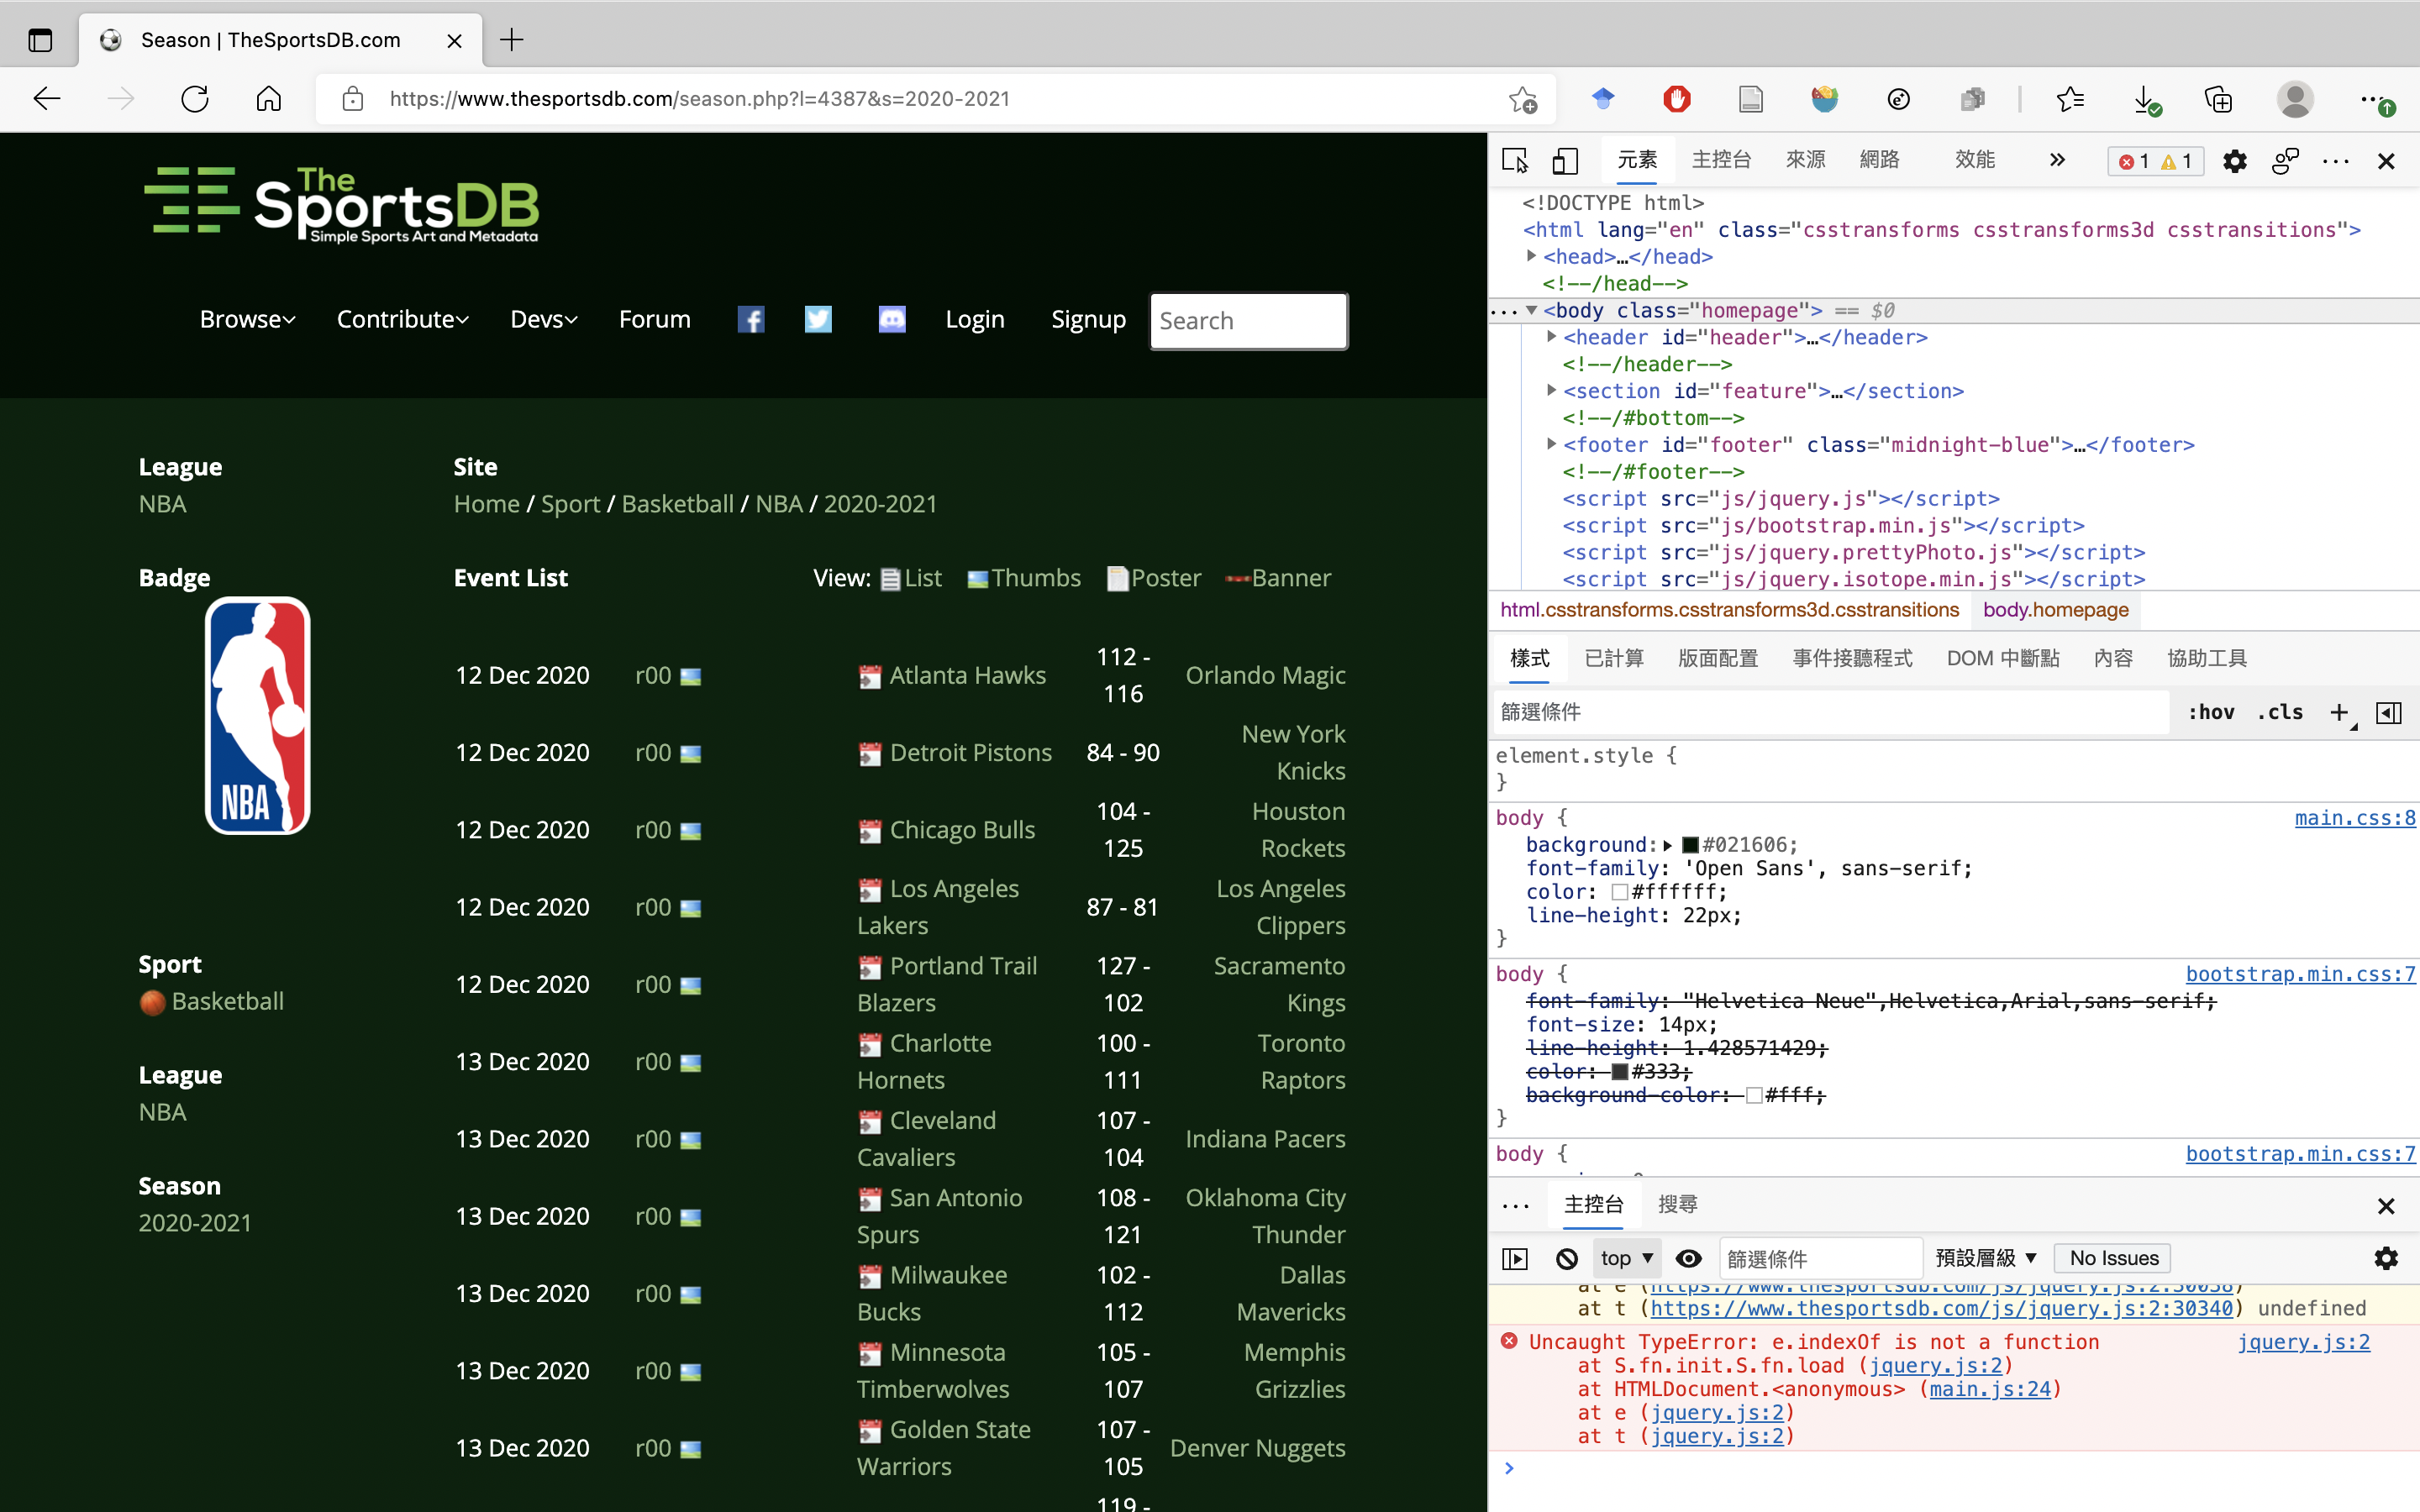
\includegraphics[width=650pt]{images/截圖 2021-07-21 上午12.26.50} 

}

\caption{Inspection menu.}\label{fig:webscraping}
\end{figure}

在 \texttt{.html} 檔中,所有元素的首尾都有一個 tag,即以 \texttt{\textless{}tag\textgreater{}} 為開頭(可能會包含屬性,如 \texttt{\textless{}tag\ attribute=value\textgreater{}}),而以 \texttt{\textless{}/tag\textgreater{}} 結尾。

在該網頁中,如圖 \ref{fig:tabletd},當我們把游標放到第一場球賽的結果時,右欄 \texttt{\textless{}td\ style="text-align:center;\ width:10\%"\textgreater{}112\ -\ 116\textless{}/td\textgreater{}} 也會被強調。在這個 tag 中,描述了文字的對齊方式與要呈現哪些文字在螢幕上。

\begin{figure}

{\centering 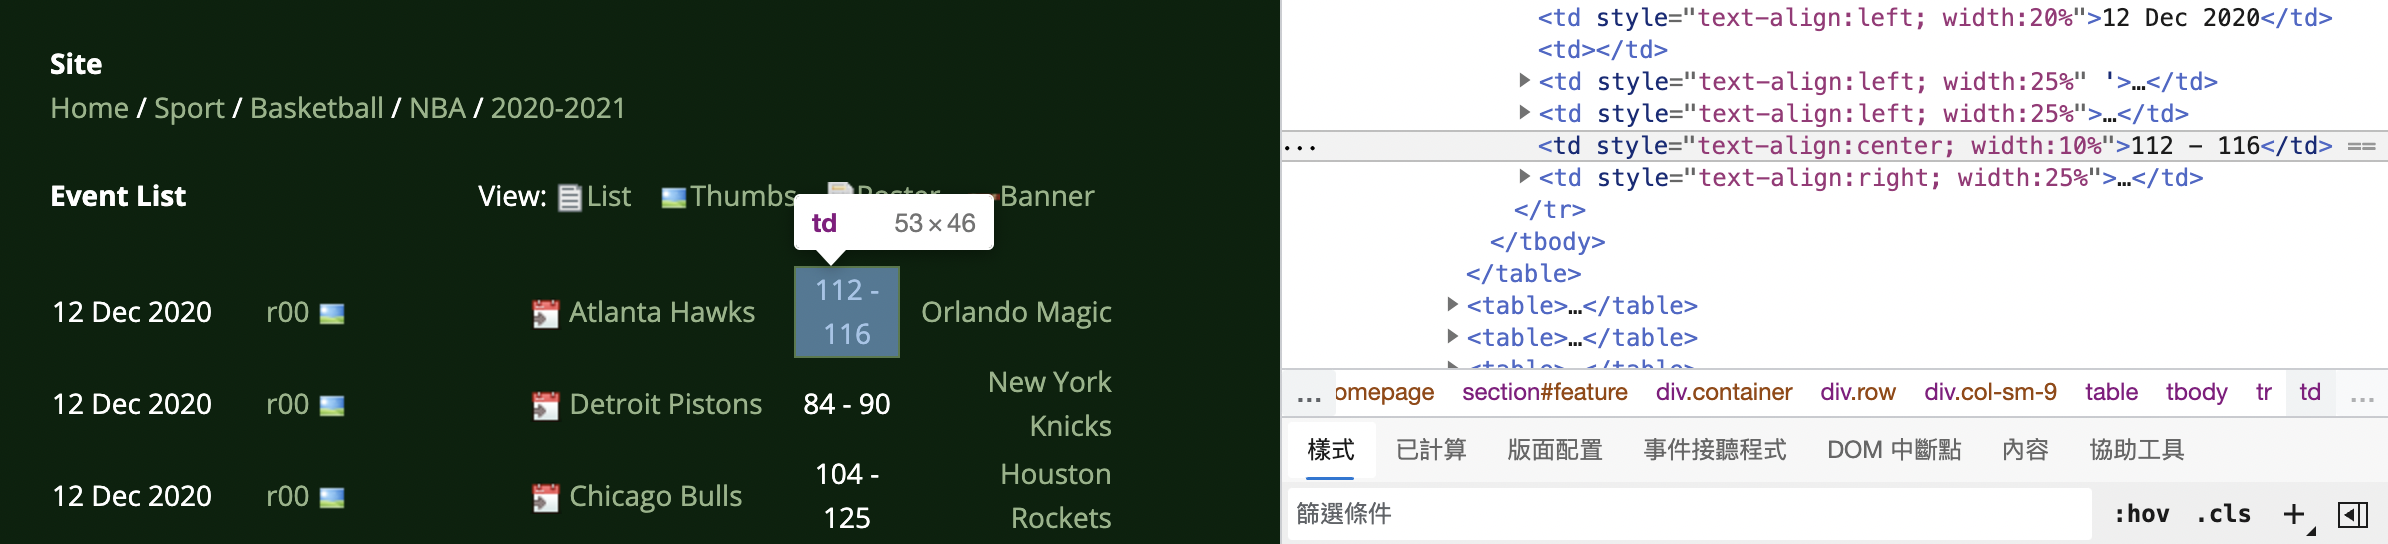
\includegraphics[width=650pt]{images/截圖 2021-07-21 上午1.25.09} 

}

\caption{第一場比賽的比分所對應到的程式碼。}\label{fig:tabletd}
\end{figure}

了解我們所要的資訊所對應到的程式碼是哪部分以後,下一個步驟是用 R 打開網頁,並告訴它要存取哪部分的資料。接下來的流程是:

\begin{enumerate}
\def\labelenumi{\arabic{enumi}.}
\tightlist
\item
  呼叫網頁,並將其存在變數中。
\item
  指定要抓取的部分。
\item
  轉換資訊成文字。
\end{enumerate}

首先使用套件 \texttt{rvest},用以擷取網頁資料。在 Console 輸入:

\begin{Shaded}
\begin{Highlighting}[]
\FunctionTok{library}\NormalTok{(rvest)}
\end{Highlighting}
\end{Shaded}

並以指令 \texttt{read\_html()} 呼叫網頁,將其儲存在變數中,如:

\begin{Shaded}
\begin{Highlighting}[]
\NormalTok{nbagames }\OtherTok{\textless{}{-}} \FunctionTok{read\_html}\NormalTok{(}\StringTok{"https://www.thesportsdb.com/season.php?l=4387\&s=2020{-}2021"}\NormalTok{)}
\end{Highlighting}
\end{Shaded}

輸入 \texttt{nbagames} 我們可以看到:

\begin{verbatim}
{html_document}
<html>
[1] <head>\n<meta http-equiv="Content-Type" content="text/html; charset=UTF-8">\n<script type="text/ja ...
[2] <body class="homepage">\n\n<header id="header"><nav class="navbar navbar-inverse" role="banner"><d ...
\end{verbatim}

而我們可以利用 \texttt{html\_nodes()} 指定要抓取的部分。此函數需要兩個引數,其一為網頁(剛剛把網頁存到的變數就要放在這裡),其二為我們所需要的 tag 的字串,因為我們需要 \texttt{\textless{}td\textgreater{}} 這個 tag,所以在這裡即輸入 \texttt{"td"},如:

\begin{Shaded}
\begin{Highlighting}[]
\NormalTok{games }\OtherTok{\textless{}{-}} \FunctionTok{html\_nodes}\NormalTok{(nbagames,}\StringTok{"td"}\NormalTok{)}
\end{Highlighting}
\end{Shaded}

此時,變數 \texttt{games} 儲存了:

\begin{verbatim}
{xml_nodeset (7327)}
 [1] <td><br></td>\n
 [2] <td style="text-align:left; width:20%">12 Dec 2020</td>\n
 [3] <td></td>\n
...
\end{verbatim}

由此可見,匯入了所有 td tags,而儲存於 \texttt{xml\_nodeset},一種專為與 \texttt{.html} 互動而設計的資料型態。因為要轉換成 \texttt{character} 才能處理,所以我們要使用 \texttt{html\_text()},如:

\begin{Shaded}
\begin{Highlighting}[]
\NormalTok{games }\OtherTok{\textless{}{-}} \FunctionTok{html\_text}\NormalTok{(}\FunctionTok{html\_nodes}\NormalTok{(nbagames, }\StringTok{"td"}\NormalTok{))}
\end{Highlighting}
\end{Shaded}

此時,\texttt{games} 內儲存的就會是:

\begin{verbatim}
[1] ""                         "12 Dec 2020"              ""                        
[4] "\n\t\t\t\t\n\t\t\t\tr00 " "Atlanta Hawks"            "112 - 116"               
[7] " Orlando Magic"           "12 Dec 2020"              ""                        
[10] "\n\t\t\t\t\n\t\t\t\tr00 " "Detroit Pistons"          "84 - 90"                 
[13] " New York Knicks"         "12 Dec 2020"              ""        
...
\end{verbatim}

可以發現,此時還是有一些空字串與 \texttt{\textbackslash{}n}(換新行)、\texttt{\textbackslash{}t}(表格)與 \texttt{\textbackslash{}tr00} 之類的字元。我們接下來的目標是把資訊拆開,存入不同的變數中。待到節 \ref{preprocessing} 將會處理這些問題。

\hypertarget{goodreads}{%
\subsubsection{Goodreads}\label{goodreads}}

第二個任務是 Goodreads 網頁所列的 21 世紀最佳書籍,可以參見:\url{https://www.goodreads.com/list/show/7.Best_Books_of_the_21st_Century}。首先當然是查看 \texttt{robots.txt}。因此我們要連到 \url{https://www.goodreads.com/robots.txt},可以發現有一大堆的 \texttt{Disallow}:

\begin{verbatim}
# See http://www.robotstxt.org/robotstxt.html for documentation on how to use the robots.txt file
User-agent: *
Disallow: /about/team_member/
Disallow: /admin
Disallow: /api
Disallow: /blog/list_rss
Disallow: /book/reviews/
Disallow: /book_link/follow/
...
\end{verbatim}

但並非什麼存取都是不被允許的(因為 \texttt{/} 沒有被 \texttt{Disallow}),且 \texttt{/list/} 也沒有被 \texttt{Disallow},所以還是可以抓取此網頁。而我們可以發現,第一本書的標題所對應的 \texttt{.html} 碼為 \texttt{\textless{}span\ itemprop="name"\ role="heading"\ aria-level="4"\textgreater{}Harry\ Potter\ and\ the\ Deathly\ Hallows\ (Harry\ Potter,\ \#7)\textless{}/span\textgreater{}},而 \texttt{span} 這個 tag 就是對應到書名。因此我們似乎可以仿效之前的做法:

\begin{Shaded}
\begin{Highlighting}[]
\NormalTok{goodreadsurl }\OtherTok{\textless{}{-}} \StringTok{"https://www.goodreads.com/list/show/7.Best\_Books\_of\_the\_21st\_Century"}
\NormalTok{goodreads }\OtherTok{\textless{}{-}} \FunctionTok{read\_html}\NormalTok{(goodreadsurl)}
\NormalTok{books }\OtherTok{\textless{}{-}} \FunctionTok{html\_text}\NormalTok{(}\FunctionTok{html\_nodes}\NormalTok{(goodreads, }\StringTok{"span"}\NormalTok{))}
\end{Highlighting}
\end{Shaded}

但我們將會發現,存進 \texttt{books} 的卻是:

\begin{verbatim}
 [1] "Browse ▾"                                                          
 [2] "Community ▾"                                                       
 [3] ""                                                                  
 [4] ""                                                                  
 [5] ""                                                                  
 [6] ""                                                                  
 [7] "Profile"                                                           
 [8] "Groups"                                                            
 [9] "Groups"                                                            
[10] "Friends’ recommendations"                                          
[11] "Friends’ recommendations"                                          
[12] "Browse ▾"                                                          
[13] "Community ▾"                                                       
[14] "Harry Potter and the Deathly Hallows (Harry Potter, #7)"      
...
\end{verbatim}

直到第 14 個元素,才抓到第一本書的書名。現在的問題就在,tag \texttt{span} 雖然有包含書名,但還有包含許多其他的資訊。要解決這個問題,我們可以發現 tag \texttt{span} 是在 tag \texttt{a} 的下層,而 tag \texttt{a} 有一屬性為 \texttt{class="bookTitle"}。Class 在 HTML 中的用處就是用來分類 tags 的方式,所以我們可以有單一個 tag,但有不同種類的資訊。因此,我們可以把剛剛的程式碼改成:

\begin{Shaded}
\begin{Highlighting}[]
\NormalTok{goodreadsurl }\OtherTok{\textless{}{-}} \StringTok{"https://www.goodreads.com/list/show/7.Best\_Books\_of\_the\_21st\_Century"}
\NormalTok{goodreads }\OtherTok{\textless{}{-}} \FunctionTok{read\_html}\NormalTok{(goodreadsurl)}
\NormalTok{books }\OtherTok{\textless{}{-}} \FunctionTok{html\_text}\NormalTok{(}\FunctionTok{html\_nodes}\NormalTok{(goodreads, }\StringTok{".bookTitle span"}\NormalTok{))}
\end{Highlighting}
\end{Shaded}

指涉 class 的時候,前面要加上 \texttt{.},而我們可以在該引數中同時放入 classes 和 tags。上述的程式碼即選取所有有 class 為 \texttt{bookTitle} 的 nodes,而選取裡頭的 tag \texttt{span}。結果,\texttt{books} 會是:

\begin{verbatim}
  [1] "Harry Potter and the Deathly Hallows (Harry Potter, #7)"                     
  [2] "The Hunger Games (The Hunger Games, #1)"                                     
  [3] "The Kite Runner"                                                             
  [4] "The Book Thief"                                                              
  [5] "Harry Potter and the Half-Blood Prince (Harry Potter, #6)"                   
  [6] "Harry Potter and the Order of the Phoenix (Harry Potter, #5)"                
  [7] "The Help"    
...
\end{verbatim}

顯然,結果就正常許多。而我們也需要提取作者與評分的資訊,因此程式碼為:

\begin{Shaded}
\begin{Highlighting}[]
\NormalTok{goodreads }\OtherTok{\textless{}{-}} \FunctionTok{read\_html}\NormalTok{(goodreadsurl)}
\NormalTok{book }\OtherTok{\textless{}{-}} \FunctionTok{html\_text}\NormalTok{(}\FunctionTok{html\_nodes}\NormalTok{(goodreads, }\StringTok{".bookTitle span"}\NormalTok{))}
\NormalTok{author }\OtherTok{\textless{}{-}} \FunctionTok{html\_text}\NormalTok{(}\FunctionTok{html\_nodes}\NormalTok{(goodreads, }\StringTok{".authorName span"}\NormalTok{))}
\NormalTok{rating }\OtherTok{\textless{}{-}} \FunctionTok{html\_text}\NormalTok{(}\FunctionTok{html\_nodes}\NormalTok{(goodreads, }\StringTok{".minirating"}\NormalTok{))}
\NormalTok{topbooks }\OtherTok{\textless{}{-}} \FunctionTok{data.frame}\NormalTok{(book, author, rating)}
\end{Highlighting}
\end{Shaded}

這時候算是大致完成了,但評分的部分的格式還是不太行,有些多餘的 hyphen 或字詞,在節 \ref{preprocessing},將會處理這個問題。

\hypertarget{ux81faux5927ux6d3bux52d5ux5831ux540dux7cfbux7d71ux8207-css-ux9078ux64c7ux5668}{%
\subsubsection{臺大活動報名系統與 CSS 選擇器}\label{ux81faux5927ux6d3bux52d5ux5831ux540dux7cfbux7d71ux8207-css-ux9078ux64c7ux5668}}

想要找出網頁的 CSS 選擇器路徑,除了上述手動查看的方法以外,如果使用 Google chrome 系列的瀏覽器,更方便的做法是使用如 \href{https://chrome.google.com/webstore/detail/selectorgadget/mhjhnkcfbdhnjickkkdbjoemdmbfginb?hl=zh-TW}{SelectorGadget} 之類的外掛。安裝完成並開啟以後直接用滑鼠點選想要抓取的元素即可,如圖 \ref{fig:ntuevents}。而如果包含到不想要選取的元素,就點選使其變成紅色,未包含到想要選取的元素則亦再行點選之即可。之後,SelectorGadge 將會產生一組 CSS 選擇器。如我們要抓取活動的代碼,其 CSS 選擇器即 \texttt{.actID}。

\begin{figure}

{\centering 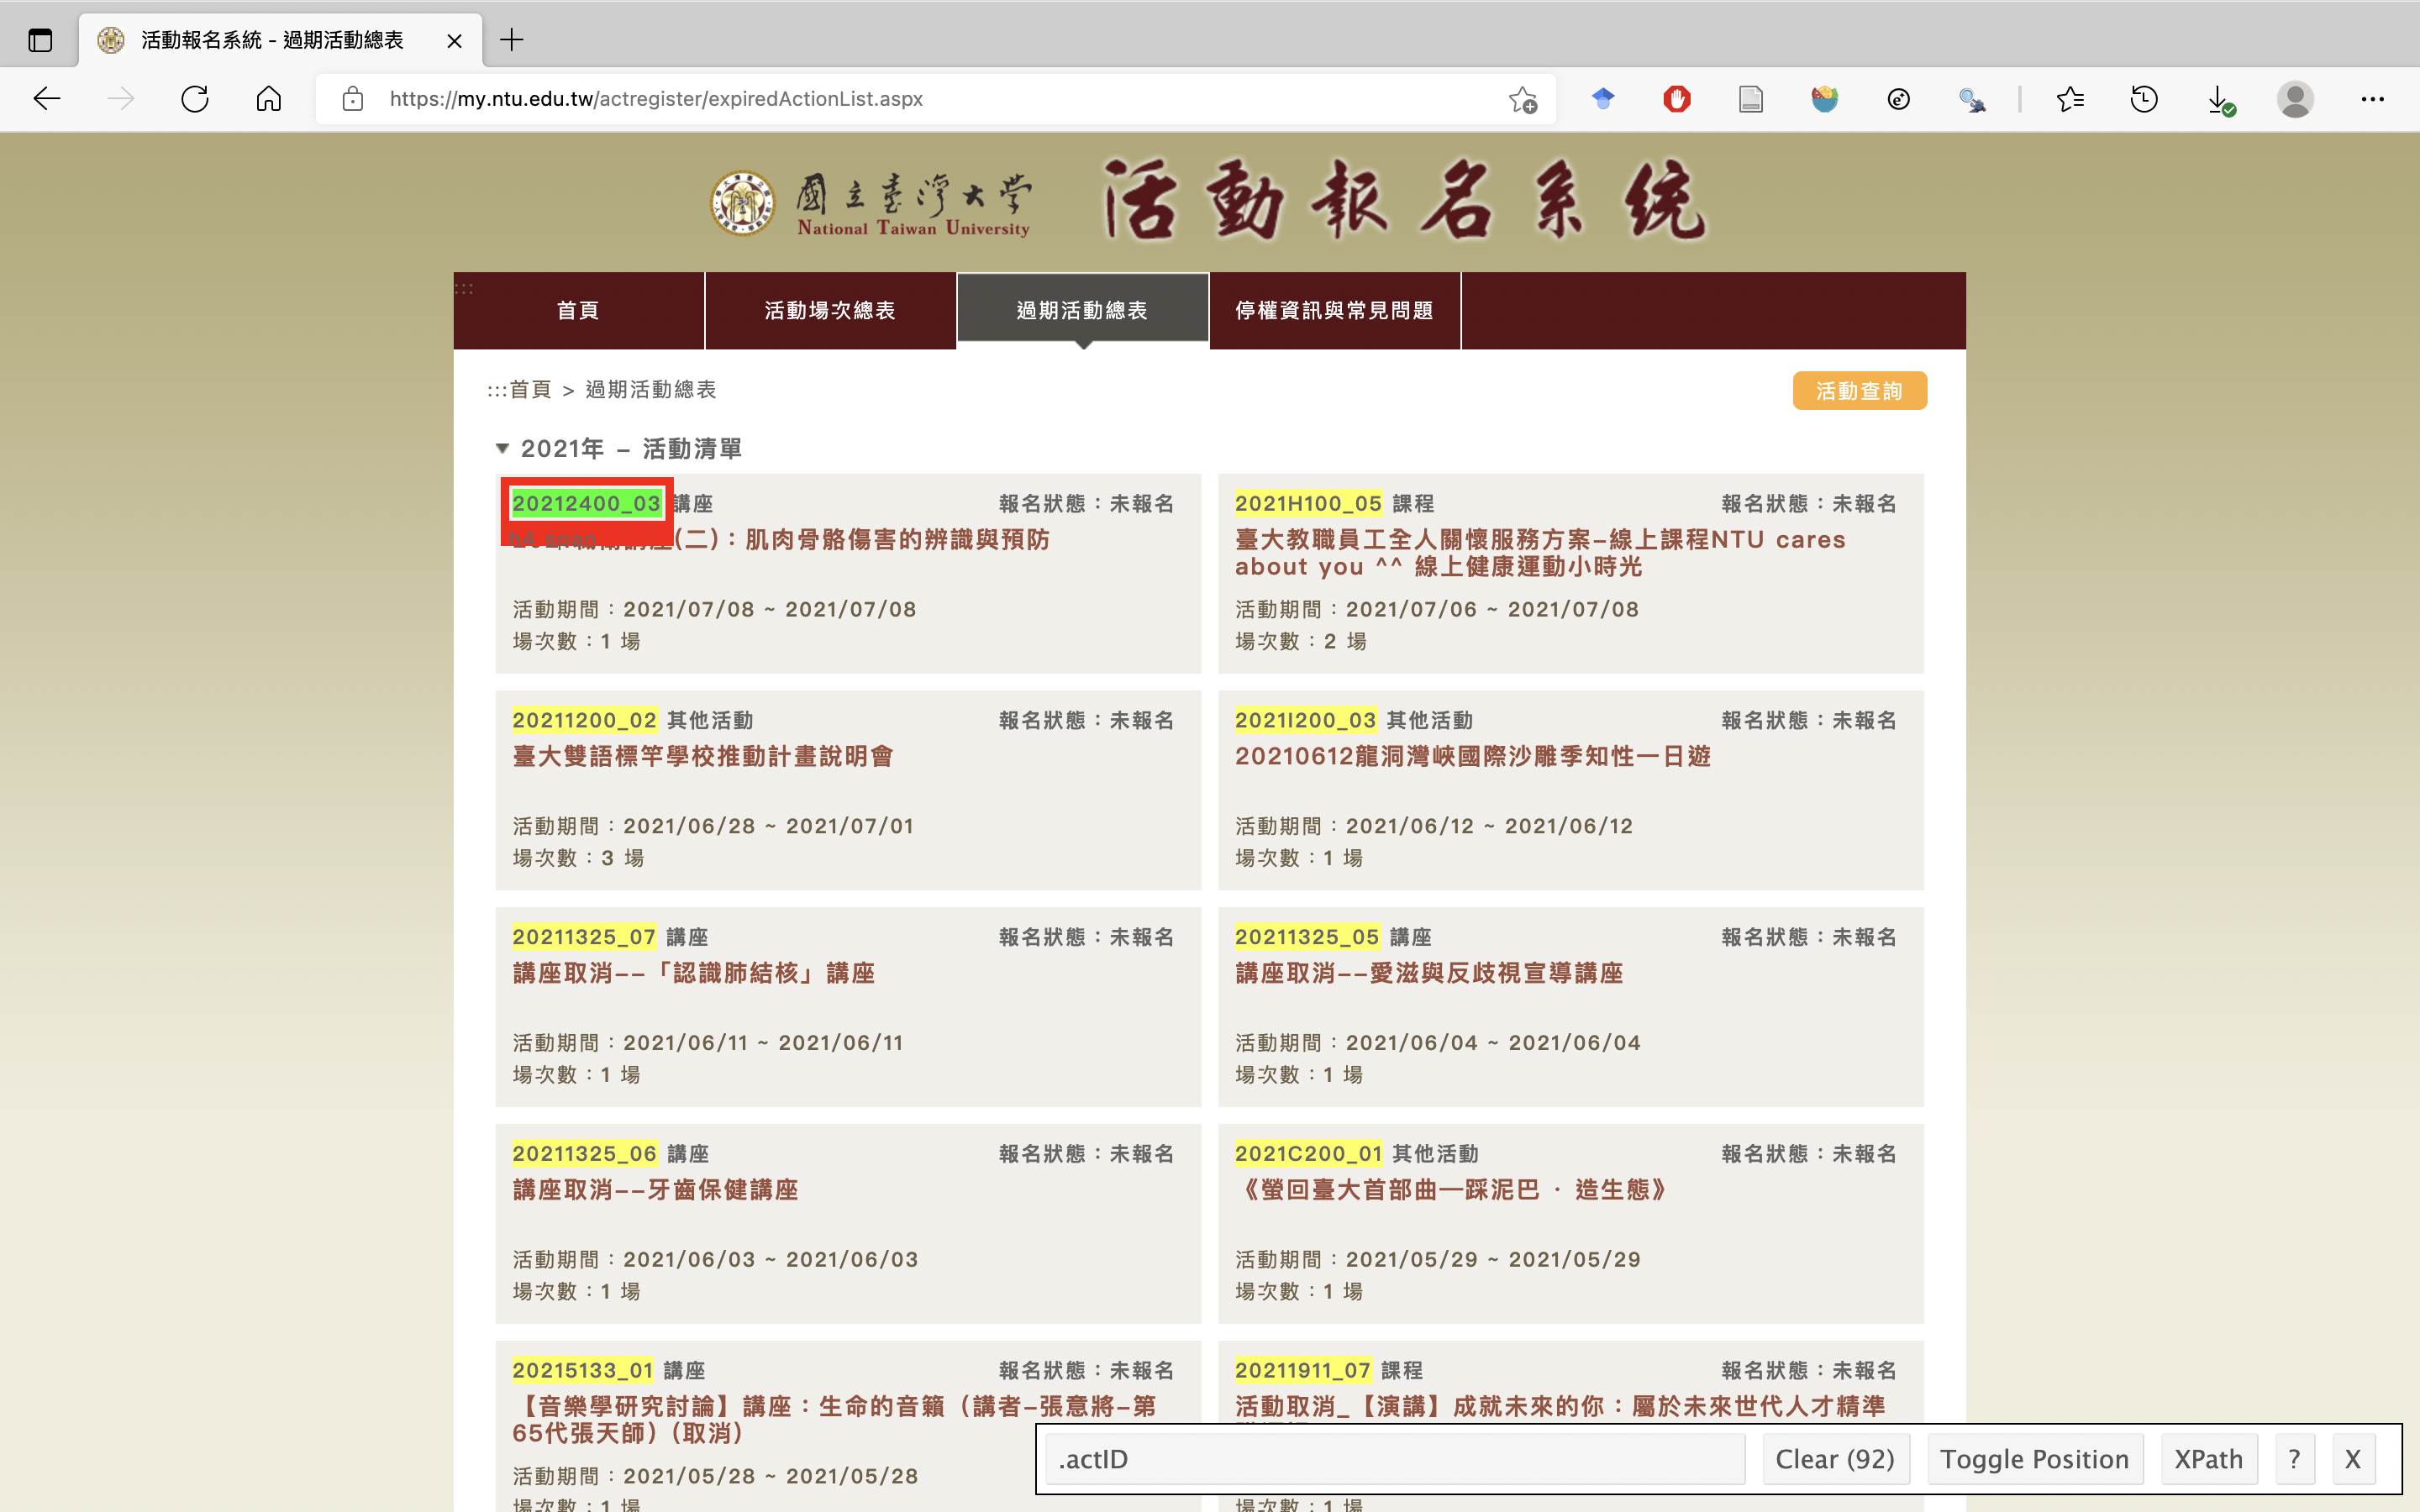
\includegraphics[width=650pt]{images/截圖 2021-07-21 下午5.52.26} 

}

\caption{使用 SelectorGadget。}\label{fig:ntuevents}
\end{figure}

因此,我們可以如此抓取臺大活動系統之過期活動中 2021 年的活動清單,並製作成一張 data table:

\begin{Shaded}
\begin{Highlighting}[]
\NormalTok{events.url }\OtherTok{\textless{}{-}} \StringTok{"https://my.ntu.edu.tw/actregister/expiredActionList.aspx"}
\NormalTok{events }\OtherTok{\textless{}{-}} \FunctionTok{read\_html}\NormalTok{(events.url)}
\NormalTok{events.number }\OtherTok{\textless{}{-}} \FunctionTok{html\_text}\NormalTok{(}\FunctionTok{html\_nodes}\NormalTok{(events, }\StringTok{".actID"}\NormalTok{))}
\NormalTok{events.name }\OtherTok{\textless{}{-}} \FunctionTok{html\_text}\NormalTok{(}\FunctionTok{html\_nodes}\NormalTok{(events, }\StringTok{".multiline"}\NormalTok{))}
\NormalTok{events.time }\OtherTok{\textless{}{-}} \FunctionTok{html\_text}\NormalTok{(}\FunctionTok{html\_nodes}\NormalTok{(events, }\StringTok{".actTime"}\NormalTok{))}
\NormalTok{events.state }\OtherTok{\textless{}{-}} \FunctionTok{html\_text}\NormalTok{(}\FunctionTok{html\_nodes}\NormalTok{(events, }\StringTok{"\#ulbox .floatRight"}\NormalTok{))}
\NormalTok{events.table }\OtherTok{\textless{}{-}} \FunctionTok{data.table}\NormalTok{(events.number, events.name, events.time, events.state)}
\end{Highlighting}
\end{Shaded}

結果如圖 \ref{fig:ntueventstable}。

\begin{figure}

{\centering 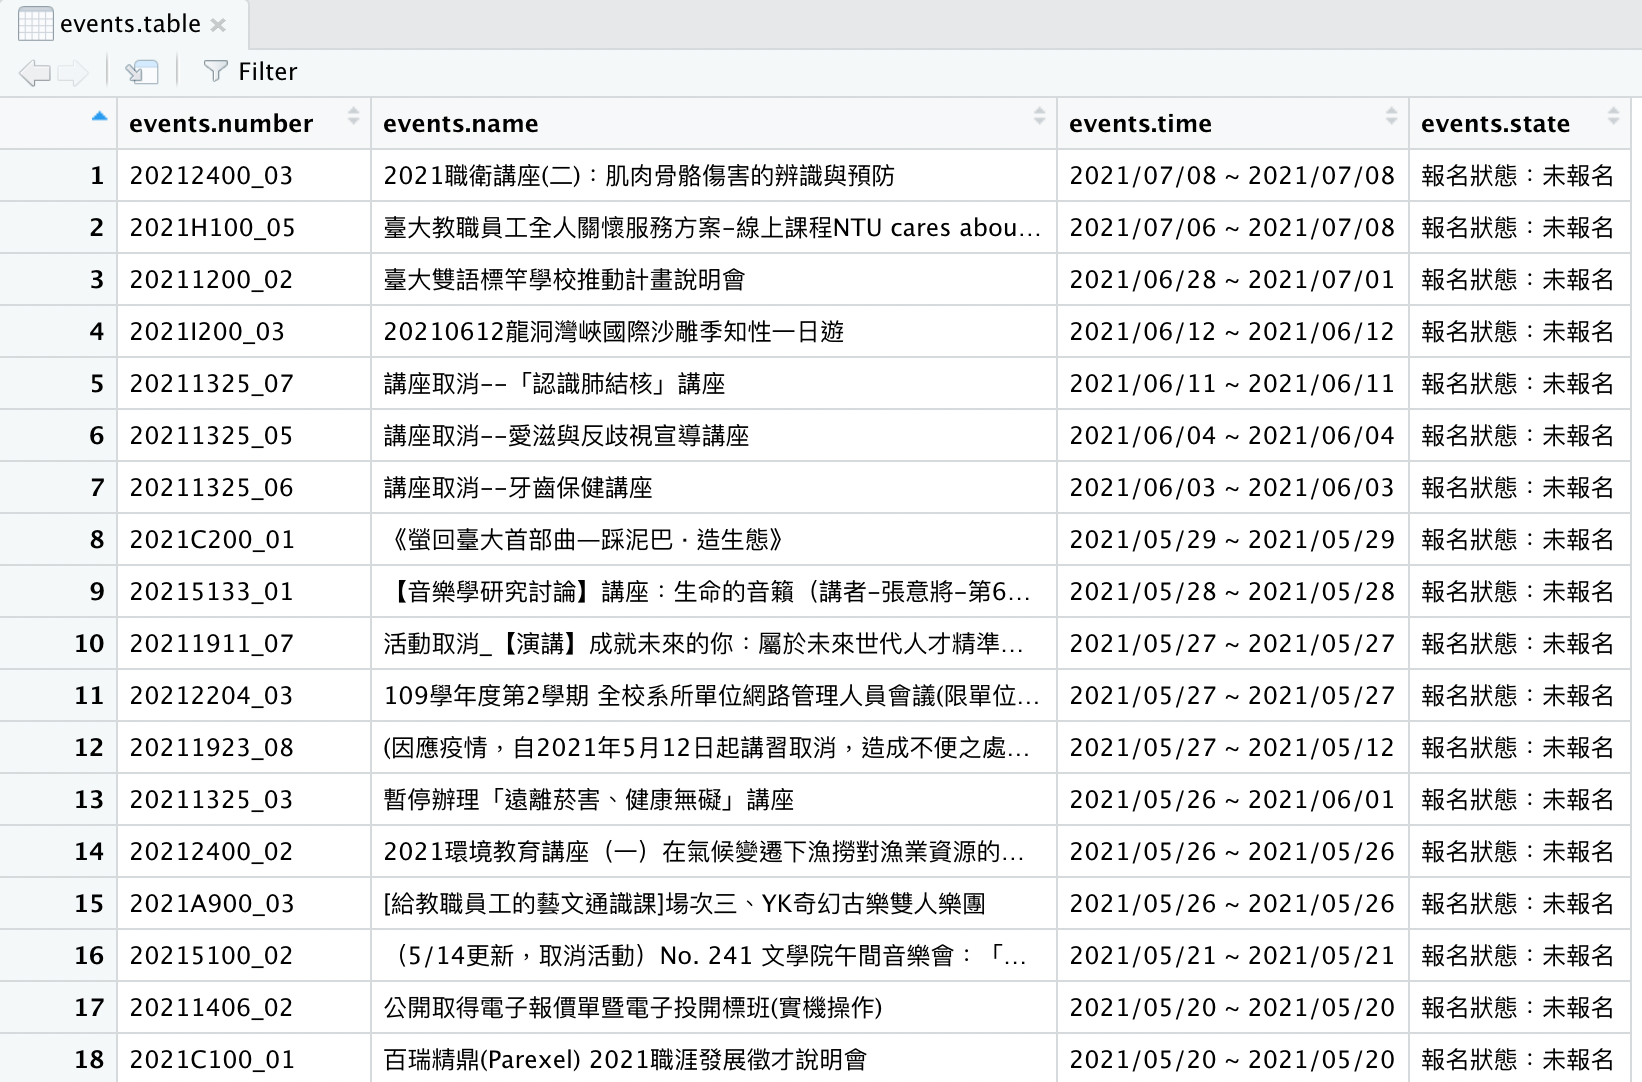
\includegraphics[width=650pt]{images/截圖 2021-07-21 下午6.07.38} 

}

\caption{抓取臺大活動系統中 2021 年的過期活動的資訊。}\label{fig:ntueventstable}
\end{figure}

\hypertarget{ux81faux5927ux653fux6cbbux7cfbux5c08ux4efbux6559ux5e2bux8cc7ux6599ux7c21ux8868}{%
\subsubsection{臺大政治系專任教師資料簡表}\label{ux81faux5927ux653fux6cbbux7cfbux5c08ux4efbux6559ux5e2bux8cc7ux6599ux7c21ux8868}}

\begin{Shaded}
\begin{Highlighting}[]
\FunctionTok{library}\NormalTok{(data.table)}
\NormalTok{polisci.prof.url }\OtherTok{\textless{}{-}} \StringTok{"http://politics.ntu.edu.tw/?cat=8"}
\NormalTok{polisci.prof }\OtherTok{\textless{}{-}} \FunctionTok{read\_html}\NormalTok{(polisci.prof.url)}
\NormalTok{prof.name }\OtherTok{\textless{}{-}} \FunctionTok{html\_text}\NormalTok{(}\FunctionTok{html\_nodes}\NormalTok{(polisci.prof, }\StringTok{".name a"}\NormalTok{))}
\NormalTok{prof.title }\OtherTok{\textless{}{-}} \FunctionTok{html\_text}\NormalTok{(}\FunctionTok{html\_nodes}\NormalTok{(polisci.prof, }\StringTok{".title"}\NormalTok{))}
\NormalTok{prof.phone }\OtherTok{\textless{}{-}} \FunctionTok{html\_text}\NormalTok{(}\FunctionTok{html\_nodes}\NormalTok{(polisci.prof, }\StringTok{".tel"}\NormalTok{))}
\NormalTok{prof.email }\OtherTok{\textless{}{-}} \FunctionTok{html\_text}\NormalTok{(}\FunctionTok{html\_nodes}\NormalTok{(polisci.prof, }\StringTok{".mail a"}\NormalTok{))}
\NormalTok{prof.table }\OtherTok{\textless{}{-}} \FunctionTok{data.table}\NormalTok{(prof.name, prof.title, prof.email)}
\NormalTok{prof.phone }\OtherTok{\textless{}{-}} \FunctionTok{append}\NormalTok{(prof.phone, }\ConstantTok{NA}\NormalTok{, }\DecValTok{13}\NormalTok{)  }\CommentTok{\# 蕭高彥沒有放電話}
\NormalTok{prof.table }\OtherTok{\textless{}{-}} \FunctionTok{cbind}\NormalTok{(prof.table, }\FunctionTok{as.data.table}\NormalTok{(prof.phone))}
\end{Highlighting}
\end{Shaded}

\begin{Shaded}
\begin{Highlighting}[]
\NormalTok{knitr}\SpecialCharTok{::}\FunctionTok{kable}\NormalTok{(prof.table, }\AttributeTok{booktabs =} \ConstantTok{TRUE}\NormalTok{, }\AttributeTok{caption =} \StringTok{\textquotesingle{}臺大政治系專任教師資料簡表。\textquotesingle{}}\NormalTok{)}
\end{Highlighting}
\end{Shaded}

\begin{table}

\caption{\label{tab:unnamed-chunk-111}臺大政治系專任教師資料簡表。}
\centering
\begin{tabular}[t]{llll}
\toprule
prof.name & prof.title & prof.email & prof.phone\\
\midrule
張登及 & 系主任 & tchang@ntu.edu.tw & 3366-8374\\
陳思賢 & 教授 & genesis@ntu.edu.tw & 3366-8320\\
黃錦堂 & 教授 & hwngntn@ntu.edu.tw & 3366-8313\\
石之瑜 & 教授 & cyshih@ntu.edu.tw & 3366-8316\\
蘇彩足 & 教授 & tsaitsu@ntu.edu.tw & 3366-8418\\
\addlinespace
朱雲漢 & 教授 & yunhan@gate.sinica.edu.tw & 3366-8397\\
吳玉山 & 教授 & yushanwu@gate.sinica.edu.tw & 3366-8381\\
王業立 & 教授 & ylwang2008@ntu.edu.tw & 3366-8413\\
蘇宏達 & 教授 & hdsu@ntu.edu.tw & 3366-8357\\
林俊宏 & 教授 & demian@ntu.edu.tw & 3366-8419\\
\addlinespace
陳淳文 & 教授 & chwenwen@ntu.edu.tw & 3366-8362\\
徐斯勤 & 教授 & schsu01@ntu.edu.tw & 3366-8406\\
張佑宗 & 教授 & yutzung@ntu.edu.tw & 3366-8399\\
左正東 & 教授 & ctso@ntu.edu.tw & NA\\
蕭高彥 & 教授 & carl@gate.sinica.edu.tw & 3366-8355\\
\addlinespace
黃長玲 & 教授 & changling@ntu.edu.tw & 3366-8347\\
黃旻華 & 教授 & mhhuang5103@ntu.edu.tw & 3366-8396\\
陶儀芬 & 副教授 & yftao@ntu.edu.tw & 3366-8420\\
陳世民 & 副教授 & shihmin@ntu.edu.tw & 3366-8350\\
林子倫 & 副教授 & tllin@ntu.edu.tw & 3366-8405\\
\addlinespace
王宏文 & 副教授 & hongwung@ntu.edu.tw & 3366-8403\\
李鳳玉 & 副教授 & fylee323@ntu.edu.tw & 3366-8321\\
郭乃菱 & 副教授 & nailing@ntu.edu.tw & 3366-8323\\
唐欣偉 & 副教授 & hsinweitang@ntu.edu.tw & 3366-8417\\
蔡季廷 & 副教授 & chiting@ntu.edu.tw & 3366-8305\\
\addlinespace
黃心怡 & 副教授 & hsinihuang@ntu.edu.tw & 3366-8366\\
劉康慧 & 副教授 & helenliu4@ntu.edu.tw & 3366-8382\\
童涵浦 & 副教授 & hanstung@ntu.edu.tw & 3366-8402\\
洪美仁 & 副教授 & meijhung@ntu.edu.tw & 3366-8304\\
郭銘峰 & 副教授 & mingfeng.kuo@gmail.com & 3366-8385\\
\addlinespace
黃凱苹 & 助理教授 & kaipinghuang@ntu.edu.tw & 3366-8387\\
廖小娟 & 助理教授 & mandyliao@ntu.edu.tw & 3366-8325\\
安井伸介 & 助理教授 & anjing@ntu.edu.tw & 3366-8336\\
郭銘傑 & 助理教授 & jasonkuo@g.ntu.edu.tw & 3366-8333\\
吳舜文 & 助理教授 & shunwu@ntu.edu.tw & 3366-8309\\
\addlinespace
張貴閔 & 助理教授 & changkueimin@ntu.edu.tw & 3366-8312\\
蘇翊豪 & 助理教授 & yihaosu@ntu.edu.tw & 3366-8331\\
\bottomrule
\end{tabular}
\end{table}

\hypertarget{ux5c0fux7d50}{%
\section{小結}\label{ux5c0fux7d50}}

此外,還有兩個抓取網頁上的困難,此處沒有提及:

\begin{enumerate}
\def\labelenumi{\arabic{enumi}.}
\tightlist
\item
  有些網頁在點擊之後會產生改變,但其網址並不會改變。此外,有些資訊需要登入才能存取。而有些網頁在 \texttt{html} 之上又使用 \texttt{javascript}。上述的問題都無法透過 \texttt{rvest} 來解決。雖然有其他套件,如 \texttt{rselenium} 可以解決這些問題,但並不簡單。
\item
  此外,有些平臺不想讓資訊流出給外人使用,會去偵測並阻斷自動抓取,這時候就很難從中提取有用的資訊。
\end{enumerate}

\hypertarget{preprocessing}{%
\chapter{資料前處理}\label{preprocessing}}

在資料分析前,我們須先進行資料前處理(data preprocessing)。準備資料有以下幾個步驟(雖然並非都是永遠需要):

\begin{enumerate}
\def\labelenumi{\arabic{enumi}.}
\item
  \textbf{Cleaning:} 改變 dataset 的變數的格式。例如清除節 \ref{goodreads} 中的 \texttt{rating} 變數中無用的字元。
\item
  \textbf{Integration:} 從不同處來的資訊,在清潔以後,要整合成一張 data frame。
\item
  \textbf{Transformation:} 創造一些需要的變數,重構 dataset 成為更便於分析的格式。
\item
  \textbf{Reduction:} 如果 dataset 很龐大,而要從事的分析只是一小部分的資料,就要刪除一些變數,以釋出記憶體。
\end{enumerate}

此章將專於使用 \texttt{base} 與 \texttt{data.table};當然,也可以使用 \texttt{tidyr}、\texttt{dplyr}、\texttt{stringr} 或 \texttt{stringi};\footnote{Fast data lookups in R: dplyr vs data.table. \url{https://www.r-bloggers.com/2017/03/fast-data-lookups-in-r-dplyr-vs-data-table/}}本書第 \ref{dplyr}、\ref{tidyr}、\ref{stringr} 章將會分別介紹 \texttt{dplyr}、\texttt{tidyr} 與 \texttt{stringr}。

\hypertarget{datatable}{%
\section{Data Tables}\label{datatable}}

Data Tables 即 data frames 的改良版,效能更高、功能更多、速度更好。並且,一個 \texttt{data.table} 物件也同時是一個 \texttt{data.frame} 物件,所以前者也可以使用後者的語法。要將向量或矩陣轉換為 data table 可以使用 \texttt{as.data.table()},即:

\begin{Shaded}
\begin{Highlighting}[]
\NormalTok{our.matrix.DT }\OtherTok{\textless{}{-}} \FunctionTok{as.data.table}\NormalTok{(our.matrix)}
\end{Highlighting}
\end{Shaded}

而既存的 data frame 或 list 可以使用 \texttt{setDT()} 將其轉換成 data table(雖然也可以使用 \texttt{as.data.table()},但前者使用較少記憶體,速度更快)。不過,data table 的 row 沒有名字,所以如果要把有名字的 data frame 轉換成 data table,要使用 \texttt{keep.rownames=T} 引數,新增一個名為 \texttt{rn} 的 column,例如:

\begin{Shaded}
\begin{Highlighting}[]
\FunctionTok{library}\NormalTok{(data.table)}
\NormalTok{example }\OtherTok{\textless{}{-}} \FunctionTok{data.frame}\NormalTok{(}\AttributeTok{info1 =} \FunctionTok{c}\NormalTok{(}\DecValTok{1}\NormalTok{, }\DecValTok{2}\NormalTok{), }\AttributeTok{info2 =} \FunctionTok{c}\NormalTok{(}\StringTok{"a"}\NormalTok{, }\StringTok{"b"}\NormalTok{))}
\FunctionTok{row.names}\NormalTok{(example) }\OtherTok{\textless{}{-}} \FunctionTok{c}\NormalTok{(}\StringTok{"line1"}\NormalTok{, }\StringTok{"line2"}\NormalTok{)}
\FunctionTok{setDT}\NormalTok{(example, }\AttributeTok{keep.rownames=}\NormalTok{T)}
\end{Highlighting}
\end{Shaded}

\begin{Shaded}
\begin{Highlighting}[]
\FunctionTok{class}\NormalTok{(example)}
\end{Highlighting}
\end{Shaded}

\begin{verbatim}
## [1] "data.table" "data.frame"
\end{verbatim}

而 \texttt{data.table} 物件有如 \texttt{example.data{[}i,\ j,\ by{]}} 的格式,此三個引數分別代表 row、column 與「分類依據」。

\hypertarget{ux6392ux5e8f-ordering}{%
\subsection{排序 Ordering}\label{ux6392ux5e8f-ordering}}

要重新排序 data table 的 row 除了可以用節 \ref{dataframeordering} 的 data frame 的方法以外,還有更簡單、快速的語法。以內置的套件 \texttt{datasets} 中的 \texttt{swiss} 為例。為了避免與原本的 dataset 混淆,我們可以創建一個複本。然後將其轉換成 data table,並以城鎮名稱字母序排列(現在城鎮名為新創的 \texttt{rn} column):

\begin{Shaded}
\begin{Highlighting}[]
\NormalTok{DT.swiss }\OtherTok{\textless{}{-}} \FunctionTok{copy}\NormalTok{(swiss)}
\FunctionTok{setDT}\NormalTok{(DT.swiss, }\AttributeTok{keep.rownames=}\NormalTok{T)}
\NormalTok{DT.swiss[}\FunctionTok{order}\NormalTok{(rn)]}
\end{Highlighting}
\end{Shaded}

我們也可以依據多個變數來排列。\texttt{order()} 中的第一個引數會優先排列,如果值相等,再依據第二個引數排列,依此類推。而 \texttt{-} 為降冪排列之義。

\begin{Shaded}
\begin{Highlighting}[]
\NormalTok{DT.swiss[}\FunctionTok{order}\NormalTok{(Education, }\SpecialCharTok{{-}}\NormalTok{Agriculture)]}
\end{Highlighting}
\end{Shaded}

\hypertarget{ux5b50ux96c6-subsetting}{%
\subsection{子集 Subsetting}\label{ux5b50ux96c6-subsetting}}

如節 \ref{dataframesubsetting} 一樣存取 data frame 中的元素,我們依樣畫葫蘆來存取 data table 內的元素。例如我們如果想要存取前三個 rows 與前三個 columns 的元素,可以:

\begin{Shaded}
\begin{Highlighting}[]
\NormalTok{DT.swiss[}\DecValTok{1} \SpecialCharTok{:} \DecValTok{3}\NormalTok{, }\DecValTok{1} \SpecialCharTok{:} \DecValTok{3}\NormalTok{]}
\end{Highlighting}
\end{Shaded}

也可以使用名字來選取,如:

\begin{Shaded}
\begin{Highlighting}[]
\NormalTok{DT.swiss[}\DecValTok{1} \SpecialCharTok{:} \DecValTok{3}\NormalTok{, }\StringTok{"rn"}\NormalTok{]}
\CommentTok{\# 顯示第一至三個 rows 與名為 rn 的 column}
\end{Highlighting}
\end{Shaded}

或者使用 \texttt{!} 來不選取某個名字的 column,如:

\begin{Shaded}
\begin{Highlighting}[]
\NormalTok{DT.swiss[}\DecValTok{1} \SpecialCharTok{:} \DecValTok{3}\NormalTok{, }\SpecialCharTok{!}\StringTok{"Agriculture"}\NormalTok{]}
\CommentTok{\# 顯示第一至三個 rows,不顯示名為 Agriculture 的 column}
\end{Highlighting}
\end{Shaded}

如果使用 \texttt{-} 在數字前,則可以選取那個 row 或 column,如:

\begin{Shaded}
\begin{Highlighting}[]
\NormalTok{DT.swiss[}\SpecialCharTok{{-}}\NormalTok{(}\DecValTok{2} \SpecialCharTok{:} \DecValTok{47}\NormalTok{),]  }\CommentTok{\# 只會選取第一個 row}
\NormalTok{DT.swiss[, }\SpecialCharTok{{-}}\DecValTok{1}\NormalTok{]  }\CommentTok{\# 不選取第一個 column}
\end{Highlighting}
\end{Shaded}

或者以 \texttt{c()} 包裹的任何組合:

\begin{Shaded}
\begin{Highlighting}[]
\NormalTok{DT.swiss[}\DecValTok{1} \SpecialCharTok{:} \DecValTok{3}\NormalTok{, }\FunctionTok{c}\NormalTok{(}\StringTok{"rn"}\NormalTok{, }\StringTok{"Education"}\NormalTok{, }\StringTok{"Catholic"}\NormalTok{)]}
\CommentTok{\#  顯示第一至三個 rows,與名為 rn、Education、Catholic 的 columns}
\end{Highlighting}
\end{Shaded}

我們也可以使用 \texttt{our.data{[}condition\ on\ certain\ variables{]}} 來選取滿足條件的 rows(類似節 \ref{dataframesubsetting} 提及的 \texttt{subset()},但以 data table 速度更快)。如要找到 \texttt{Education} 恰等於 9 的城鎮,可以:

\begin{Shaded}
\begin{Highlighting}[]
\NormalTok{DT.swiss[Education }\SpecialCharTok{==} \DecValTok{9}\NormalTok{]}
\end{Highlighting}
\end{Shaded}

其結果為:

\begin{verbatim}
           rn Fertility Agriculture Examination Education Catholic Infant.Mortality
1:   Delemont      83.1        45.1           6         9    84.84             22.2
2:     Lavaux      65.1        73.0          19         9     2.84             20.0
3: St Maurice      65.0        75.9           9         9    99.06             17.8
\end{verbatim}

或者要找到 \texttt{Education} 小於等於 2 的城鎮,可以:

\begin{Shaded}
\begin{Highlighting}[]
\NormalTok{DT.swiss[Education }\SpecialCharTok{\textless{}=} \DecValTok{2}\NormalTok{]}
\end{Highlighting}
\end{Shaded}

其結果為:

\begin{verbatim}
          rn Fertility Agriculture Examination Education Catholic Infant.Mortality
1: Echallens      68.3        72.6          18         2    24.20             21.2
2:      Oron      72.5        71.2          12         1     2.40             21.0
3:   Conthey      75.5        85.9           3         2    99.71             15.1
4:    Herens      77.3        89.7           5         2   100.00             18.3
\end{verbatim}

以邏輯條件選取 data table 中的元素時,也可以超過一個條件,如:

\begin{Shaded}
\begin{Highlighting}[]
\NormalTok{mean.values }\OtherTok{\textless{}{-}} \FunctionTok{sapply}\NormalTok{(DT.swiss[, }\SpecialCharTok{{-}}\DecValTok{1}\NormalTok{], mean)}
\NormalTok{DT.swiss[Agriculture }\SpecialCharTok{\textgreater{}}\NormalTok{ mean.values[}\DecValTok{2}\NormalTok{] }\SpecialCharTok{\&}\NormalTok{ Education }\SpecialCharTok{\textgreater{}}\NormalTok{ mean.values[}\DecValTok{4}\NormalTok{]]}
\end{Highlighting}
\end{Shaded}

回憶節 \ref{defaultargument} 所提及的,\texttt{sapply(list,\ function)} 可以套用函數在多個元素上,並輸出為向量或矩陣。\texttt{sapply(DT.swiss{[},\ -1{]},\ mean)} 之義為套用 \texttt{mean()} 這個函數在 \texttt{DT.swiss} 中除了第一個 column 以外的其他 columns,即算出其平均值,並輸出成有標籤的向量。而我們將輸出的資料存入 \texttt{mean.values} 變數中。如此,我們就能找出同時滿足「\texttt{Agriculure} 與 \texttt{Education} 皆大於平均值」的 rows,即:

\begin{verbatim}
         rn Fertility Agriculture Examination Education Catholic Infant.Mortality
1:    Aigle      64.1        62.0          21        12     8.52             16.5
2: Avenches      68.9        60.7          19        12     4.43             22.7
3:    Nyone      56.6        50.9          22        12    15.14             16.7
4:     Sion      79.3        63.1          13        13    96.83             18.1
\end{verbatim}

另一個 data table 的優勢是第二個引數 \texttt{j} 其實可以傳入非索引值的物件,例如我們想知道 \texttt{Catholic\ \textgreater{}\ 50} 的城鎮其 \texttt{Education} 的平均可以透過:

\begin{Shaded}
\begin{Highlighting}[]
\NormalTok{DT.swiss[Catholic }\SpecialCharTok{\textgreater{}} \DecValTok{50}\NormalTok{, }\FunctionTok{mean}\NormalTok{(Education)]}
\end{Highlighting}
\end{Shaded}

\begin{verbatim}
## [1] 9.111111
\end{verbatim}

也可以知道 \texttt{Catholic\ \textgreater{}\ 50} 的城鎮其 \texttt{Education} 的平均是否大於整體的 \texttt{Education} 平均:

\begin{Shaded}
\begin{Highlighting}[]
\NormalTok{DT.swiss[Catholic }\SpecialCharTok{\textgreater{}} \DecValTok{50}\NormalTok{, }\FunctionTok{mean}\NormalTok{(Education) }\SpecialCharTok{\textgreater{}}\NormalTok{ mean.values[}\DecValTok{4}\NormalTok{]]}
\end{Highlighting}
\end{Shaded}

\begin{verbatim}
## Education 
##     FALSE
\end{verbatim}

或者 \texttt{Education} 小於 10 的城鎮究竟有多少:

\begin{Shaded}
\begin{Highlighting}[]
\NormalTok{DT.swiss[Education }\SpecialCharTok{\textless{}} \DecValTok{10}\NormalTok{, }\FunctionTok{length}\NormalTok{(Education)]}
\end{Highlighting}
\end{Shaded}

\begin{verbatim}
## [1] 28
\end{verbatim}

\hypertarget{ux52a0ux7e3d-aggregation}{%
\subsection{加總 Aggregation}\label{ux52a0ux7e3d-aggregation}}

前面曾經提及,\texttt{example.data{[}i,\ j,\ by{]}} 中的引數 \texttt{by} 為分組依據。其使用要配合引數 \texttt{j}。例如我們想得知每一個 \texttt{Education} 的值所對應到的 \texttt{Fertility} 的平均值,並且依據 \texttt{Education} 降冪排列,可以:

\begin{Shaded}
\begin{Highlighting}[]
\NormalTok{DT.swiss[}\FunctionTok{order}\NormalTok{(}\SpecialCharTok{{-}}\NormalTok{Education), }\FunctionTok{mean}\NormalTok{(Fertility), by}\OtherTok{=}\NormalTok{Education]}
\end{Highlighting}
\end{Shaded}

\begin{verbatim}
    Education       V1
 1:        53 35.00000
 2:        32 64.40000
 3:        29 43.75000
 4:        28 55.70000
 5:        20 54.30000
 ...
\end{verbatim}

當使用 \texttt{by} 來分類時,在引數 \texttt{j} 就無法使用 \texttt{length()} 來計算出現次數了。這時候可以改用 \texttt{.N} 來計算各組的數字,如:

\begin{Shaded}
\begin{Highlighting}[]
\NormalTok{DT.swiss[}\FunctionTok{order}\NormalTok{(}\SpecialCharTok{{-}}\NormalTok{Education), .N, by}\OtherTok{=}\NormalTok{Education]}
\end{Highlighting}
\end{Shaded}

\begin{verbatim}
    Education N
 1:        53 1
 2:        32 1
 3:        29 2
 4:        28 1
 5:        20 1
 ...
\end{verbatim}

也可以與 \texttt{maen()} 結合起來,以下列出各 \texttt{Education} 程度的數量,並分別算出各 \texttt{Education} 程度的 \texttt{Fertility} 與 \texttt{Catholic} 的平均,而以 \texttt{Education} 降冪排列:

\begin{Shaded}
\begin{Highlighting}[]
\NormalTok{DT.swiss[}\FunctionTok{order}\NormalTok{(}\SpecialCharTok{{-}}\NormalTok{Education), .(.N, }\FunctionTok{mean}\NormalTok{(Fertility), }\FunctionTok{mean}\NormalTok{(Catholic)), by}\OtherTok{=}\NormalTok{Education]}
\end{Highlighting}
\end{Shaded}

\begin{verbatim}
   Education N       V2       V3
 1:        53 1 35.00000 42.34000
 2:        32 1 64.40000 16.92000
 3:        29 2 43.75000 54.38000
 4:        28 1 55.70000 12.11000
 5:        20 1 54.30000  2.15000
...
\end{verbatim}

除此之外,\texttt{by} 也可以丟入邏輯式,如:

\begin{Shaded}
\begin{Highlighting}[]
\NormalTok{DT.swiss[, .N, .(Education }\SpecialCharTok{\textless{}} \DecValTok{15}\NormalTok{, Fertility }\SpecialCharTok{\textgreater{}} \DecValTok{60}\NormalTok{)]}
\end{Highlighting}
\end{Shaded}

\begin{verbatim}
   Education Fertility  N
1:      TRUE      TRUE 37
2:     FALSE      TRUE  2
3:     FALSE     FALSE  6
4:      TRUE     FALSE  2
\end{verbatim}

我們可以得知,有 37 個城鎮的 \texttt{Education} 小於 15,且 \texttt{Fertility} 大於 60;2 個城鎮的 \texttt{Education} 不小於 15,且 \texttt{Fertility} 大於 60;有 6 個城鎮的 \texttt{Education} 不小於 15,且 \texttt{Fertility} 不大於 60;2 個城鎮的 \texttt{Education} 小於 15,且 \texttt{Fertility} 不大於 60。

\hypertarget{keying}{%
\subsection{Keying}\label{keying}}

Keys 是另一個選取子集(subsetting)更快的方法。只要在 data table 的某個變數中設定了 key,表格在物理上就會重新排列記憶體與儲存的 rows 所分派的順序。設定 key 的指令為 \texttt{setkey(data.table,\ key)},如:

\begin{Shaded}
\begin{Highlighting}[]
\FunctionTok{setkey}\NormalTok{(DT.swiss, Education)}
\end{Highlighting}
\end{Shaded}

之後,表格就會依據 \texttt{Education} 重新排列:

\begin{verbatim}
              rn Fertility Agriculture Examination Education Catholic Infant.Mortality
 1:         Oron      72.5        71.2          12         1     2.40             21.0
 2:    Echallens      68.3        72.6          18         2    24.20             21.2
 3:      Conthey      75.5        85.9           3         2    99.71             15.1
 4:       Herens      77.3        89.7           5         2   100.00             18.3
 5:       Moudon      65.0        55.1          14         3     4.52             22.4
 6: Paysd'enhaut      72.0        63.5           6         3     2.56             18.0
 7:      Monthey      79.4        64.9           7         3    98.22             20.2
...
\end{verbatim}

想要 subsetting keyed variable,可以使用 \texttt{.()},如下列出 \texttt{Education} 等於 3 的 rows:

\begin{Shaded}
\begin{Highlighting}[]
\NormalTok{DT.swiss[.(}\DecValTok{3}\NormalTok{)]}
\end{Highlighting}
\end{Shaded}

\begin{verbatim}
##              rn Fertility Agriculture Examination Education Catholic
## 1:       Moudon      65.0        55.1          14         3     4.52
## 2: Paysd'enhaut      72.0        63.5           6         3     2.56
## 3:      Monthey      79.4        64.9           7         3    98.22
## 4:       Sierre      92.2        84.6           3         3    99.46
##    Infant.Mortality
## 1:             22.4
## 2:             18.0
## 3:             20.2
## 4:             16.3
\end{verbatim}

也可以輸入向量,如下列出 \texttt{Education} 等於 3 或 5 的 rows:

\begin{Shaded}
\begin{Highlighting}[]
\NormalTok{DT.swiss[.(}\FunctionTok{c}\NormalTok{(}\DecValTok{3}\NormalTok{, }\DecValTok{5}\NormalTok{))]}
\end{Highlighting}
\end{Shaded}

\begin{verbatim}
##              rn Fertility Agriculture Examination Education Catholic
## 1:       Moudon      65.0        55.1          14         3     4.52
## 2: Paysd'enhaut      72.0        63.5           6         3     2.56
## 3:      Monthey      79.4        64.9           7         3    98.22
## 4:       Sierre      92.2        84.6           3         3    99.46
## 5: Franches-Mnt      92.5        39.7           5         5    93.40
## 6:     Cossonay      61.7        69.3          22         5     2.82
##    Infant.Mortality
## 1:             22.4
## 2:             18.0
## 3:             20.2
## 4:             16.3
## 5:             20.2
## 6:             18.7
\end{verbatim}

也可以與引數\texttt{j} 和 \texttt{by} 搭配使用,如:

\begin{Shaded}
\begin{Highlighting}[]
\NormalTok{DT.swiss[.(}\DecValTok{1} \SpecialCharTok{:} \DecValTok{2}\NormalTok{), }\SpecialCharTok{!}\FunctionTok{c}\NormalTok{(}\StringTok{"Agriculture"}\NormalTok{, }\StringTok{"Infant.Mortality"}\NormalTok{)]}
\end{Highlighting}
\end{Shaded}

\begin{verbatim}
##           rn Fertility Examination Education Catholic
## 1:      Oron      72.5          12         1     2.40
## 2: Echallens      68.3          18         2    24.20
## 3:   Conthey      75.5           3         2    99.71
## 4:    Herens      77.3           5         2   100.00
\end{verbatim}

與:

\begin{Shaded}
\begin{Highlighting}[]
\NormalTok{DT.swiss[.(}\DecValTok{3} \SpecialCharTok{:} \DecValTok{6}\NormalTok{), }\FunctionTok{mean}\NormalTok{(Fertility), by}\OtherTok{=}\NormalTok{Education]}
\end{Highlighting}
\end{Shaded}

\begin{verbatim}
##    Education     V1
## 1:         3 77.150
## 2:        NA     NA
## 3:         5 77.100
## 4:         6 71.075
\end{verbatim}

\hypertarget{ux7de8ux8f2fux8868ux683c-updating-by-reference}{%
\subsection{編輯表格 Updating by Reference}\label{ux7de8ux8f2fux8868ux683c-updating-by-reference}}

那如何編輯表格呢?使用 \texttt{:=},之前放 column 的名字,而之後放要指派的值。如果要新增兩個 column,可以:

\begin{Shaded}
\begin{Highlighting}[]
\NormalTok{DT.swiss[, }\FunctionTok{c}\NormalTok{(}\StringTok{"new.col.1"}\NormalTok{, }\StringTok{"new.col.2"}\NormalTok{)}\SpecialCharTok{:}\ErrorTok{=}\FunctionTok{list}\NormalTok{(}\DecValTok{1} \SpecialCharTok{:} \DecValTok{47}\NormalTok{, }\DecValTok{51} \SpecialCharTok{:} \DecValTok{97}\NormalTok{)]}
\end{Highlighting}
\end{Shaded}

其結果為:

\begin{verbatim}
              rn Fertility Agriculture Examination Education Catholic Infant.Mortality new.col.1 new.col.2
 1:         Oron      72.5        71.2          12         1     2.40             21.0         1        51
 2:    Echallens      68.3        72.6          18         2    24.20             21.2         2        52
 3:      Conthey      75.5        85.9           3         2    99.71             15.1         3        53
 4:       Herens      77.3        89.7           5         2   100.00             18.3         4        54
 5:       Moudon      65.0        55.1          14         3     4.52             22.4         5        55
...
46:    Neuchatel      64.4        17.6          35        32    16.92             23.0        46        96
47: V. De Geneve      35.0         1.2          37        53    42.34             18.0        47        97
\end{verbatim}

修改其值也如同剛才的做法:

\begin{Shaded}
\begin{Highlighting}[]
\NormalTok{DT.swiss[, }\FunctionTok{c}\NormalTok{(}\StringTok{"new.col.1"}\NormalTok{, }\StringTok{"new.col.2"}\NormalTok{)}\SpecialCharTok{:}\ErrorTok{=}\FunctionTok{list}\NormalTok{(}\DecValTok{101} \SpecialCharTok{:} \DecValTok{147}\NormalTok{, }\DecValTok{151} \SpecialCharTok{:} \DecValTok{197}\NormalTok{)]}
\end{Highlighting}
\end{Shaded}

結果為:

\begin{verbatim}
              rn Fertility Agriculture Examination Education Catholic Infant.Mortality new.col.1 new.col.2
 1:         Oron      72.5        71.2          12         1     2.40             21.0       101       151
 2:    Echallens      68.3        72.6          18         2    24.20             21.2       102       152
 3:      Conthey      75.5        85.9           3         2    99.71             15.1       103       153
 4:       Herens      77.3        89.7           5         2   100.00             18.3       104       154
 5:       Moudon      65.0        55.1          14         3     4.52             22.4       105       155
...
46:    Neuchatel      64.4        17.6          35        32    16.92             23.0       146       196
47: V. De Geneve      35.0         1.2          37        53    42.34             18.0       147       197
\end{verbatim}

如果要刪除既存的 column,則可以:

\begin{Shaded}
\begin{Highlighting}[]
\NormalTok{DT.swiss[, }\FunctionTok{c}\NormalTok{(}\StringTok{"new.col.1"}\NormalTok{, }\StringTok{"new.col.2"}\NormalTok{)}\SpecialCharTok{:}\ErrorTok{=}\FunctionTok{list}\NormalTok{(}\ConstantTok{NULL}\NormalTok{, }\ConstantTok{NULL}\NormalTok{)]}
\end{Highlighting}
\end{Shaded}

\hypertarget{merging}{%
\section{Merging}\label{merging}}

如果兩個 data table 有一樣的變數,那要合併可以使用 \texttt{rbind()}(row binding),如:

\begin{Shaded}
\begin{Highlighting}[]
\NormalTok{dataset}\FloatTok{.1} \OtherTok{\textless{}{-}} \FunctionTok{data.table}\NormalTok{(}\AttributeTok{city=}\FunctionTok{c}\NormalTok{(}\StringTok{"Large"}\NormalTok{, }\StringTok{"Medium"}\NormalTok{), }\AttributeTok{population=}\FunctionTok{c}\NormalTok{(}\DecValTok{1000000}\NormalTok{, }\DecValTok{250000}\NormalTok{), }\AttributeTok{km2=}\FunctionTok{c}\NormalTok{(}\DecValTok{20}\NormalTok{, }\DecValTok{7}\NormalTok{))}
\NormalTok{dataset}\FloatTok{.2} \OtherTok{\textless{}{-}} \FunctionTok{data.table}\NormalTok{(}\AttributeTok{city=}\FunctionTok{c}\NormalTok{(}\StringTok{"Small"}\NormalTok{), }\AttributeTok{population=}\FunctionTok{c}\NormalTok{(}\DecValTok{50000}\NormalTok{), }\AttributeTok{km2=}\FunctionTok{c}\NormalTok{(}\DecValTok{1}\NormalTok{))}
\NormalTok{dataset.final }\OtherTok{\textless{}{-}} \FunctionTok{rbind}\NormalTok{(dataset}\FloatTok{.1}\NormalTok{, dataset}\FloatTok{.2}\NormalTok{)}
\NormalTok{dataset.final}
\end{Highlighting}
\end{Shaded}

\begin{verbatim}
##      city population km2
## 1:  Large    1000000  20
## 2: Medium     250000   7
## 3:  Small      50000   1
\end{verbatim}

如果有相同多的觀察值,則使用 \texttt{cbind()}(column binding),例如:

\begin{Shaded}
\begin{Highlighting}[]
\NormalTok{dataset}\FloatTok{.1} \OtherTok{\textless{}{-}} \FunctionTok{data.table}\NormalTok{(}\AttributeTok{city=}\FunctionTok{c}\NormalTok{(}\StringTok{"Large"}\NormalTok{, }\StringTok{"Medium"}\NormalTok{, }\StringTok{"Small"}\NormalTok{), }\AttributeTok{population=}\FunctionTok{c}\NormalTok{(}\DecValTok{1000000}\NormalTok{, }\DecValTok{250000}\NormalTok{, }\DecValTok{50000}\NormalTok{))}
\NormalTok{dataset}\FloatTok{.2} \OtherTok{\textless{}{-}} \FunctionTok{data.table}\NormalTok{(}\AttributeTok{km2=}\FunctionTok{c}\NormalTok{(}\DecValTok{20}\NormalTok{, }\DecValTok{7}\NormalTok{, }\DecValTok{1}\NormalTok{))}
\NormalTok{dataset.final }\OtherTok{\textless{}{-}} \FunctionTok{cbind}\NormalTok{(dataset}\FloatTok{.1}\NormalTok{, dataset}\FloatTok{.2}\NormalTok{)}
\NormalTok{dataset.final}
\end{Highlighting}
\end{Shaded}

\begin{verbatim}
##      city population km2
## 1:  Large    1000000  20
## 2: Medium     250000   7
## 3:  Small      50000   1
\end{verbatim}

如果兩個表格共享某些 rows 與 columns,則可以使用 \texttt{merge()},如:

\begin{Shaded}
\begin{Highlighting}[]
\NormalTok{dataset}\FloatTok{.1} \OtherTok{\textless{}{-}} \FunctionTok{data.table}\NormalTok{(}\AttributeTok{city=}\FunctionTok{c}\NormalTok{(}\StringTok{"city.1"}\NormalTok{, }\StringTok{"city.2"}\NormalTok{, }\StringTok{"city.3"}\NormalTok{, }\StringTok{"city.4"}\NormalTok{, }\StringTok{"city.5"}\NormalTok{, }\StringTok{"city.6"}\NormalTok{), }
                        \AttributeTok{population=}\FunctionTok{c}\NormalTok{(}\DecValTok{10000}\NormalTok{, }\DecValTok{20000}\NormalTok{, }\DecValTok{100000}\NormalTok{, }\DecValTok{5000}\NormalTok{, }\DecValTok{30000}\NormalTok{, }\DecValTok{65000}\NormalTok{),}
                        \AttributeTok{km2=}\FunctionTok{c}\NormalTok{(}\DecValTok{1}\NormalTok{, }\FloatTok{0.5}\NormalTok{, }\FloatTok{0.9}\NormalTok{, }\DecValTok{2}\NormalTok{, }\FloatTok{1.2}\NormalTok{, }\DecValTok{3}\NormalTok{))}
\NormalTok{dataset}\FloatTok{.2} \OtherTok{\textless{}{-}} \FunctionTok{data.table}\NormalTok{(}\AttributeTok{city=}\FunctionTok{c}\NormalTok{(}\StringTok{"city.1"}\NormalTok{, }\StringTok{"city.2"}\NormalTok{, }\StringTok{"city.3"}\NormalTok{, }\StringTok{"city.7"}\NormalTok{),}
                        \AttributeTok{airport=}\FunctionTok{c}\NormalTok{(}\ConstantTok{FALSE}\NormalTok{, }\ConstantTok{FALSE}\NormalTok{, }\ConstantTok{TRUE}\NormalTok{, }\ConstantTok{TRUE}\NormalTok{))}
\NormalTok{dataset}\FloatTok{.1}
\end{Highlighting}
\end{Shaded}

\begin{verbatim}
##      city population km2
## 1: city.1      10000 1.0
## 2: city.2      20000 0.5
## 3: city.3     100000 0.9
## 4: city.4       5000 2.0
## 5: city.5      30000 1.2
## 6: city.6      65000 3.0
\end{verbatim}

\begin{Shaded}
\begin{Highlighting}[]
\NormalTok{dataset}\FloatTok{.2}
\end{Highlighting}
\end{Shaded}

\begin{verbatim}
##      city airport
## 1: city.1   FALSE
## 2: city.2   FALSE
## 3: city.3    TRUE
## 4: city.7    TRUE
\end{verbatim}

\begin{Shaded}
\begin{Highlighting}[]
\CommentTok{\# inner join:包含所有 columns,但有缺漏值的 rows 會被跳過}
\FunctionTok{merge}\NormalTok{(dataset}\FloatTok{.1}\NormalTok{, dataset}\FloatTok{.2}\NormalTok{)}
\end{Highlighting}
\end{Shaded}

\begin{verbatim}
##      city population km2 airport
## 1: city.1      1e+04 1.0   FALSE
## 2: city.2      2e+04 0.5   FALSE
## 3: city.3      1e+05 0.9    TRUE
\end{verbatim}

\begin{Shaded}
\begin{Highlighting}[]
\CommentTok{\# full join:包含所有 columns 與 rows}
\FunctionTok{merge}\NormalTok{(dataset}\FloatTok{.1}\NormalTok{, dataset}\FloatTok{.2}\NormalTok{, }\AttributeTok{all =} \ConstantTok{TRUE}\NormalTok{)}
\end{Highlighting}
\end{Shaded}

\begin{verbatim}
##      city population km2 airport
## 1: city.1      10000 1.0   FALSE
## 2: city.2      20000 0.5   FALSE
## 3: city.3     100000 0.9    TRUE
## 4: city.4       5000 2.0      NA
## 5: city.5      30000 1.2      NA
## 6: city.6      65000 3.0      NA
## 7: city.7         NA  NA    TRUE
\end{verbatim}

\begin{Shaded}
\begin{Highlighting}[]
\CommentTok{\# left join:包含所有 columns,但跳過第一個表格沒有的 rows}
\FunctionTok{merge}\NormalTok{(dataset}\FloatTok{.1}\NormalTok{, dataset}\FloatTok{.2}\NormalTok{, }\AttributeTok{all.x =} \ConstantTok{TRUE}\NormalTok{)}
\end{Highlighting}
\end{Shaded}

\begin{verbatim}
##      city population km2 airport
## 1: city.1      10000 1.0   FALSE
## 2: city.2      20000 0.5   FALSE
## 3: city.3     100000 0.9    TRUE
## 4: city.4       5000 2.0      NA
## 5: city.5      30000 1.2      NA
## 6: city.6      65000 3.0      NA
\end{verbatim}

\begin{Shaded}
\begin{Highlighting}[]
\CommentTok{\# right join:包含所有 columns,但跳過第二個表格沒有的 rows}
\FunctionTok{merge}\NormalTok{(dataset}\FloatTok{.1}\NormalTok{, dataset}\FloatTok{.2}\NormalTok{, }\AttributeTok{all.y =} \ConstantTok{TRUE}\NormalTok{)}
\end{Highlighting}
\end{Shaded}

\begin{verbatim}
##      city population km2 airport
## 1: city.1      1e+04 1.0   FALSE
## 2: city.2      2e+04 0.5   FALSE
## 3: city.3      1e+05 0.9    TRUE
## 4: city.7         NA  NA    TRUE
\end{verbatim}

\hypertarget{ux5be6ux4f8b}{%
\section{實例}\label{ux5be6ux4f8b}}

除了前章所介紹的指令,本節還會介紹用以:

\begin{itemize}
\tightlist
\item
  資料清理的 \texttt{na.omit()}、\texttt{duplicated()};
\item
  文字轉換的 \texttt{substr()}、\texttt{tstrplit()}、\texttt{grepl()}。
\end{itemize}

\texttt{na.omit()} 可以剔除表格中有 \texttt{NA} 的觀察值(rows);\texttt{duplicated()} 則可以幫助我們刪除重複的觀察值。例如我們新建一個 data table:

\begin{Shaded}
\begin{Highlighting}[]
\NormalTok{dupli.table }\OtherTok{\textless{}{-}} \FunctionTok{data.table}\NormalTok{(}\AttributeTok{ID=}\FunctionTok{c}\NormalTok{(}\StringTok{"E123456789"}\NormalTok{, }\StringTok{"N123456789"}\NormalTok{, }\StringTok{"N213456897"}\NormalTok{, }\StringTok{"N123456789"}\NormalTok{, }\StringTok{"A123456789"}\NormalTok{, }\StringTok{"N213456897"}\NormalTok{, }\StringTok{"E213456897"}\NormalTok{), }\AttributeTok{sex=}\FunctionTok{c}\NormalTok{(}\StringTok{"M"}\NormalTok{, }\StringTok{"M"}\NormalTok{, }\StringTok{"F"}\NormalTok{, }\StringTok{"M"}\NormalTok{, }\StringTok{"M"}\NormalTok{, }\StringTok{"F"}\NormalTok{, }\StringTok{"F"}\NormalTok{), }\AttributeTok{major=}\FunctionTok{c}\NormalTok{(}\StringTok{"Econ"}\NormalTok{, }\ConstantTok{NA}\NormalTok{, }\StringTok{"Math"}\NormalTok{, }\StringTok{"OR"}\NormalTok{, }\StringTok{"EE"}\NormalTok{, }\StringTok{"CS"}\NormalTok{, }\StringTok{"Eng"}\NormalTok{))}
\end{Highlighting}
\end{Shaded}

使用 \texttt{na.omit()} 即會刪除有 \texttt{NA} 的觀察值:

\begin{Shaded}
\begin{Highlighting}[]
\NormalTok{dupli.table }\OtherTok{\textless{}{-}} \FunctionTok{na.omit}\NormalTok{(dupli.table)}
\NormalTok{dupli.table}
\end{Highlighting}
\end{Shaded}

\begin{verbatim}
##            ID sex major
## 1: E123456789   M  Econ
## 2: N213456897   F  Math
## 3: N123456789   M    OR
## 4: A123456789   M    EE
## 5: N213456897   F    CS
## 6: E213456897   F   Eng
\end{verbatim}

使用 \texttt{duplicated()} 可以協助我們找到特定的 columns 重複的觀察值,例如:

\begin{Shaded}
\begin{Highlighting}[]
\NormalTok{duplicated.rows1 }\OtherTok{\textless{}{-}} \FunctionTok{duplicated}\NormalTok{(dupli.table[, }\FunctionTok{c}\NormalTok{(}\DecValTok{1}\NormalTok{, }\DecValTok{3}\NormalTok{)])  }\CommentTok{\# 設定第一個與第三個 cols}
\CommentTok{\# 得到 "FALSE FALSE FALSE FALSE FALSE FALSE"}
\CommentTok{\# 表示完全沒有在第一個與第三個 cols 都重複的觀察值}

\NormalTok{duplicated.rows2 }\OtherTok{\textless{}{-}} \FunctionTok{duplicated}\NormalTok{(dupli.table[, }\FunctionTok{c}\NormalTok{(}\DecValTok{1}\NormalTok{, }\DecValTok{2}\NormalTok{)])  }\CommentTok{\# 設定第一個與第二個 cols}
\CommentTok{\# 得到 "FALSE FALSE FALSE FALSE  TRUE FALSE"}
\CommentTok{\# 表示第五個觀察值重複了}

\NormalTok{duplicated.rows3 }\OtherTok{\textless{}{-}} \FunctionTok{duplicated}\NormalTok{(dupli.table[, }\DecValTok{1}\NormalTok{])  }\CommentTok{\# 設定第一個 cols}
\CommentTok{\# 等價於 duplicated.rows3 \textless{}{-} duplicated(dupli.table$ID)}
\CommentTok{\# 得到 "FALSE FALSE FALSE FALSE  TRUE FALSE"}
\CommentTok{\# 表示第五個觀察值重複了}
\end{Highlighting}
\end{Shaded}

那要怎樣刪除重複的觀察值呢?我們可以:

\begin{Shaded}
\begin{Highlighting}[]
\NormalTok{dupli.table }\OtherTok{\textless{}{-}}\NormalTok{ dupli.table[}\SpecialCharTok{!}\NormalTok{duplicated.rows2]}
\NormalTok{dupli.table}
\end{Highlighting}
\end{Shaded}

\begin{verbatim}
##            ID sex major
## 1: E123456789   M  Econ
## 2: N213456897   F  Math
## 3: N123456789   M    OR
## 4: A123456789   M    EE
## 5: E213456897   F   Eng
\end{verbatim}

\hypertarget{thesportsdb-nba-dataset-preprocessing}{%
\subsection{TheSportsDB NBA Dataset Preprocessing}\label{thesportsdb-nba-dataset-preprocessing}}

上一章使用:

\begin{Shaded}
\begin{Highlighting}[]
\FunctionTok{library}\NormalTok{(rvest)}
\NormalTok{nbagames }\OtherTok{\textless{}{-}} \FunctionTok{read\_html}\NormalTok{(}\StringTok{"https://www.thesportsdb.com/season.php?l=4387\&s=2020{-}2021"}\NormalTok{)}
\NormalTok{games }\OtherTok{\textless{}{-}} \FunctionTok{html\_text}\NormalTok{(}\FunctionTok{html\_nodes}\NormalTok{(nbagames,}\StringTok{"td"}\NormalTok{))}
\end{Highlighting}
\end{Shaded}

得到的 \texttt{games} 儲存了許多無用的字元:

\begin{verbatim}
  [1] ""                         "12 Dec 2020"              ""                         "\n\t\t\t\t\n\t\t\t\tr00 "
  [5] "Atlanta Hawks"            "112 - 116"                " Orlando Magic"           "12 Dec 2020"             
  [9] ""                         "\n\t\t\t\t\n\t\t\t\tr00 " "Detroit Pistons"          "84 - 90"       
...
\end{verbatim}

首先我們要先把空的項目刪除:

\begin{Shaded}
\begin{Highlighting}[]
\NormalTok{games }\OtherTok{\textless{}{-}}\NormalTok{ games[}\SpecialCharTok{!}\NormalTok{games}\SpecialCharTok{==}\StringTok{""}\NormalTok{]}
\end{Highlighting}
\end{Shaded}

接著,我們想把包含 \texttt{\textbackslash{}n} 的項目刪除。但是,他們都長得不太一樣,於是我們要以 \texttt{grepl(text-to-find,\ where-to-find-it)} 來刪除:

\begin{Shaded}
\begin{Highlighting}[]
\NormalTok{games }\OtherTok{\textless{}{-}}\NormalTok{ games[}\SpecialCharTok{!}\FunctionTok{grepl}\NormalTok{(}\StringTok{"}\SpecialCharTok{\textbackslash{}n}\StringTok{"}\NormalTok{,games)]}
\end{Highlighting}
\end{Shaded}

現在這樣就正常很多了。而現在儲存的方式是向量,我們可以將其轉成有 4 個 column 的矩陣,然後將其轉換成 data table,並冠上 column names:

\begin{Shaded}
\begin{Highlighting}[]
\NormalTok{games}\FloatTok{.2021} \OtherTok{\textless{}{-}} \FunctionTok{as.data.table}\NormalTok{(}\FunctionTok{matrix}\NormalTok{(games, }\AttributeTok{ncol=}\DecValTok{4}\NormalTok{, }\AttributeTok{byrow=}\NormalTok{T))}
\FunctionTok{colnames}\NormalTok{(games}\FloatTok{.2021}\NormalTok{) }\OtherTok{\textless{}{-}} \FunctionTok{c}\NormalTok{(}\StringTok{"Date"}\NormalTok{,}\StringTok{"TeamA"}\NormalTok{,}\StringTok{"Result"}\NormalTok{,}\StringTok{"TeamB"}\NormalTok{)}
\end{Highlighting}
\end{Shaded}

不過,比分還是無法計算,因為現在是兩個數字。\texttt{data.table} 中的函數 \texttt{tstrsplit(variable,\ separator,\ keep)} 可以用以切開資訊,如:

\begin{Shaded}
\begin{Highlighting}[]
\NormalTok{games}\FloatTok{.2021}\NormalTok{[, }\FunctionTok{tstrsplit}\NormalTok{(Result, }\StringTok{"{-}"}\NormalTok{)]}
\CommentTok{\# 相當於 games.2021[, tstrsplit(Result, " ", keep = c(1, 3))]}
\end{Highlighting}
\end{Shaded}

\begin{verbatim}
        V1   V2
   1: 112   116
   2:  84    90
   3: 104   125
   4:  87    81
   5: 127   102
  ---          
1217: 118   108
1218: 120   100
1219: 109   103
1220: 119   123
1221: 105    98
\end{verbatim}

因此,我們如果要新增兩個 columns,分別是 A 隊與 B 隊的分數,可以:

\begin{Shaded}
\begin{Highlighting}[]
\NormalTok{games}\FloatTok{.2021}\NormalTok{[, }\FunctionTok{c}\NormalTok{(}\StringTok{"PointsA"}\NormalTok{, }\StringTok{"PointsB"}\NormalTok{)}\SpecialCharTok{:}\ErrorTok{=}\FunctionTok{tstrsplit}\NormalTok{(Result, }\StringTok{"{-}"}\NormalTok{)]}
\NormalTok{games}\FloatTok{.2021}\SpecialCharTok{$}\NormalTok{Result }\OtherTok{\textless{}{-}} \ConstantTok{NULL}
\end{Highlighting}
\end{Shaded}

得:

\begin{verbatim}
             Date                  TeamA                 TeamB PointsA PointsB
   1: 12 Dec 2020          Atlanta Hawks         Orlando Magic    112      116
   2: 12 Dec 2020        Detroit Pistons       New York Knicks     84       90
   3: 12 Dec 2020          Chicago Bulls       Houston Rockets    104      125
   4: 12 Dec 2020     Los Angeles Lakers  Los Angeles Clippers     87       81
   5: 12 Dec 2020 Portland Trail Blazers      Sacramento Kings    127      102
  ---                                                                         
1217: 09 Jul 2021           Phoenix Suns       Milwaukee Bucks    118      108
1218: 12 Jul 2021        Milwaukee Bucks          Phoenix Suns    120      100
1219: 15 Jul 2021        Milwaukee Bucks          Phoenix Suns    109      103
1220: 18 Jul 2021           Phoenix Suns       Milwaukee Bucks    119      123
1221: 21 Jul 2021        Milwaukee Bucks          Phoenix Suns    105       98
\end{verbatim}

\hypertarget{part-ux4ee5-tidyverse-ux9032ux884cux8cc7ux6599ux63a2ux7d22}{%
\chapter*{\texorpdfstring{(PART) 以 \texttt{tidyverse} 進行資料探索}{(PART) 以 tidyverse 進行資料探索}}\label{part-ux4ee5-tidyverse-ux9032ux884cux8cc7ux6599ux63a2ux7d22}}

\hypertarget{ux4ee5-ggplot2-ux9032ux884cux8cc7ux6599ux8996ux89baux5316}{%
\chapter{\texorpdfstring{以 \texttt{ggplot2} 進行資料視覺化}{以 ggplot2 進行資料視覺化}}\label{ux4ee5-ggplot2-ux9032ux884cux8cc7ux6599ux8996ux89baux5316}}

本部分要談的是資料探索。

\begin{figure}

{\centering 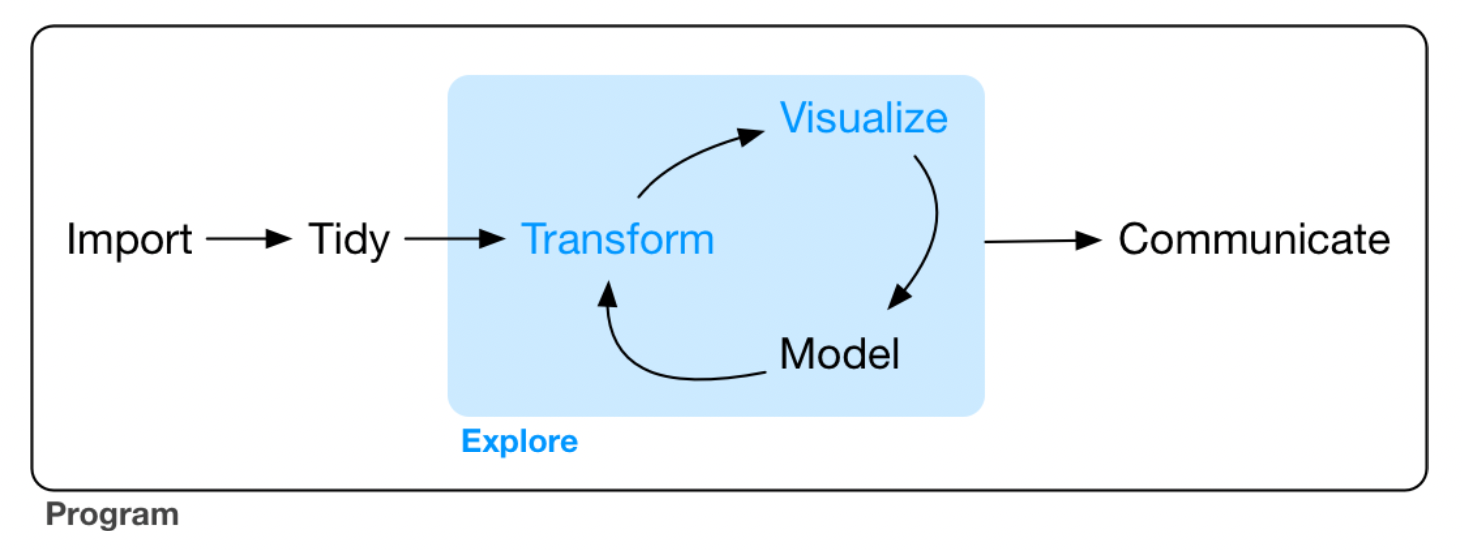
\includegraphics[width=550]{images/截圖 2021-07-24 下午3.22.11} 

}

\caption{Data exploring.}\label{fig:dataexploring}
\end{figure}

\hypertarget{ux524dux7f6eux4f5cux696d}{%
\subsubsection*{前置作業}\label{ux524dux7f6eux4f5cux696d}}
\addcontentsline{toc}{subsubsection}{前置作業}

此章的目的則是要學習以 \texttt{ggplot2} 進行簡單的資料視覺化。我們先要載入 \texttt{tidyverse},其包含了 \texttt{ggplot2}。在 Console 輸入:

\begin{Shaded}
\begin{Highlighting}[]
\FunctionTok{library}\NormalTok{(tidyverse)}
\end{Highlighting}
\end{Shaded}

\begin{verbatim}
## -- Attaching packages --------------------------------------- tidyverse 1.3.1 --
\end{verbatim}

\begin{verbatim}
## v ggplot2 3.3.5     v purrr   0.3.4
## v tibble  3.1.3     v dplyr   1.0.7
## v tidyr   1.1.3     v stringr 1.4.0
## v readr   2.0.0     v forcats 0.5.1
\end{verbatim}

\begin{verbatim}
## Warning: package 'ggplot2' was built under R version 4.1.1
\end{verbatim}

\begin{verbatim}
## -- Conflicts ------------------------------------------ tidyverse_conflicts() --
## x dplyr::between()        masks data.table::between()
## x dplyr::filter()         masks stats::filter()
## x dplyr::first()          masks data.table::first()
## x purrr::flatten()        masks jsonlite::flatten()
## x readr::guess_encoding() masks rvest::guess_encoding()
## x dplyr::lag()            masks stats::lag()
## x dplyr::last()           masks data.table::last()
## x purrr::transpose()      masks data.table::transpose()
\end{verbatim}

\hypertarget{create}{%
\section{\texorpdfstring{創建一個 \texttt{ggplot}}{創建一個 ggplot}}\label{create}}

\begin{quote}
引擎大的車子相較於引擎小的車子使用更多的汽油嗎?
\end{quote}

我們可以使用 \texttt{tidyverse} 中 \texttt{mpg} 這個 data frame 來嘗試回答這個問題。

\begin{Shaded}
\begin{Highlighting}[]
\NormalTok{mpg}
\end{Highlighting}
\end{Shaded}

\begin{verbatim}
## # A tibble: 234 x 11
##    manufacturer model      displ  year   cyl trans drv     cty   hwy fl    class
##    <chr>        <chr>      <dbl> <int> <int> <chr> <chr> <int> <int> <chr> <chr>
##  1 audi         a4           1.8  1999     4 auto~ f        18    29 p     comp~
##  2 audi         a4           1.8  1999     4 manu~ f        21    29 p     comp~
##  3 audi         a4           2    2008     4 manu~ f        20    31 p     comp~
##  4 audi         a4           2    2008     4 auto~ f        21    30 p     comp~
##  5 audi         a4           2.8  1999     6 auto~ f        16    26 p     comp~
##  6 audi         a4           2.8  1999     6 manu~ f        18    26 p     comp~
##  7 audi         a4           3.1  2008     6 auto~ f        18    27 p     comp~
##  8 audi         a4 quattro   1.8  1999     4 manu~ 4        18    26 p     comp~
##  9 audi         a4 quattro   1.8  1999     4 auto~ 4        16    25 p     comp~
## 10 audi         a4 quattro   2    2008     4 manu~ 4        20    28 p     comp~
## # ... with 224 more rows
\end{verbatim}

其中,\texttt{displ} 為引擎的大小,單位是公升數;\texttt{hwy} 為汽車在高速公路上的燃油效率,以每加侖英里(miles per gallon, mpg)為單位,較低的話代表同樣的里程得要使用更多的油。

我們可以把 \texttt{displ} 放在 \(x\) 軸,而把 \texttt{hwy} 放在 \(y\) 軸,創建一個 \texttt{ggplot}:

\begin{Shaded}
\begin{Highlighting}[]
\FunctionTok{ggplot}\NormalTok{(}\AttributeTok{data =}\NormalTok{ mpg) }\SpecialCharTok{+} \FunctionTok{geom\_point}\NormalTok{(}\AttributeTok{mapping =} \FunctionTok{aes}\NormalTok{(}\AttributeTok{x =}\NormalTok{ displ, }\AttributeTok{y =}\NormalTok{ hwy))}
\end{Highlighting}
\end{Shaded}

\begin{center}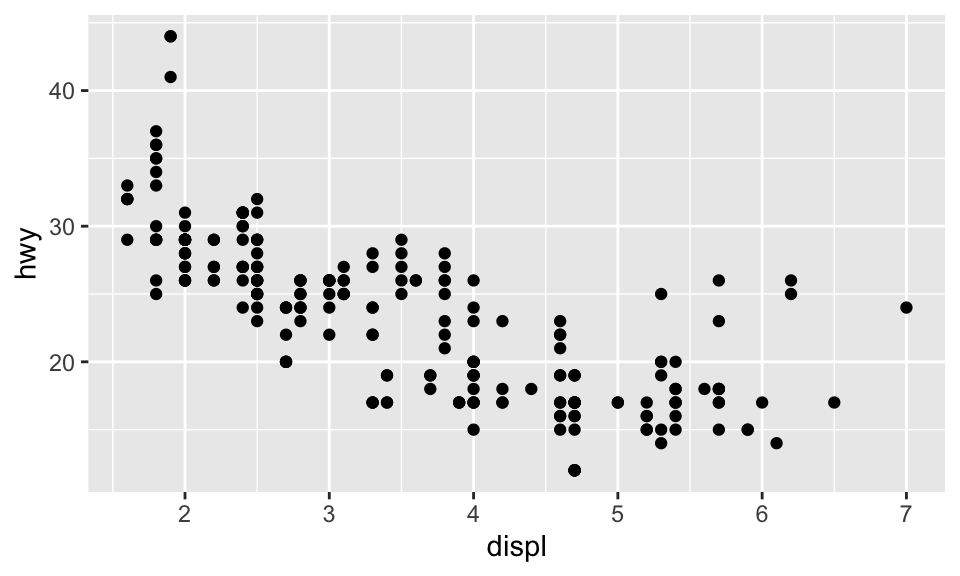
\includegraphics{R_learing_notes_files/figure-latex/unnamed-chunk-155-1} \end{center}

\texttt{ggplot()} 可以創造一個座標系統,而我們可以在上面加上圖層。其中,第一個引數為此圖所要使用的 dataset,例如此處為 \texttt{ggplot(dataset=mpg)},但這時候不會得到任何東西,只有一張空白的圖。而我們可以再加上其他圖層,如使用 \texttt{geom\_point()},可以用來繪製散佈圖(scatterplot)。而 \texttt{geom\_point()} 函數有引數 \texttt{mapping},與 \texttt{aes()} 搭配使用,可以讓我們指定 \(x\) 軸與 \(y\) 軸分別要是什麼變數。

此外,從此圖看起來,引擎大小與燃油效率呈現負向關係,即引擎更大的車,使用更多油。

\hypertarget{the-layered-grammar-of-graphics}{%
\section{The Layered Grammar of Graphics}\label{the-layered-grammar-of-graphics}}

\texttt{ggplot2} 的語法大致如下,層層堆疊各種函數。在 geom 中,除了 \texttt{mapping=aes()},我們還可以加上其他種類的 \texttt{stat} 與 ``position adjustment'';若有需要,也可以加上不同的「座標系統」與 ``facet function''。

\begin{Shaded}
\begin{Highlighting}[]
\FunctionTok{ggplot}\NormalTok{(}\AttributeTok{data =} \SpecialCharTok{\textless{}}\NormalTok{DATA}\SpecialCharTok{\textgreater{}}\NormalTok{) }\SpecialCharTok{+} 
  \ErrorTok{\textless{}}\NormalTok{GEOM\_FUNCTION}\SpecialCharTok{\textgreater{}}\NormalTok{(}
    \AttributeTok{mapping =} \FunctionTok{aes}\NormalTok{(}\SpecialCharTok{\textless{}}\NormalTok{MAPPINGS}\SpecialCharTok{\textgreater{}}\NormalTok{),}
    \AttributeTok{stat =} \SpecialCharTok{\textless{}}\NormalTok{STAT}\SpecialCharTok{\textgreater{}}\NormalTok{,}
    \AttributeTok{position =} \SpecialCharTok{\textless{}}\NormalTok{POSITION}\SpecialCharTok{\textgreater{}}\NormalTok{)}\SpecialCharTok{+}
    \ErrorTok{\textless{}}\NormalTok{COORDINATE\_FUNCTION}\SpecialCharTok{\textgreater{}} \SpecialCharTok{+}
    \ErrorTok{\textless{}}\NormalTok{FACET\_FUNCTION}\SpecialCharTok{\textgreater{}}
\end{Highlighting}
\end{Shaded}

以下將逐一簡介這些參數(以 \texttt{\textless{}\textgreater{}} 包圍的字串)的使用方式。

\hypertarget{aesthetic-mappings}{%
\section{Aesthetic Mappings}\label{aesthetic-mappings}}

我們可以新增第三個變數,例如 \texttt{mpg} 中的 \texttt{class} 到兩向度的散佈圖,讓上面的點映射到 \emph{aesthetic}。\emph{Aesthetic} 是一種物件的視覺性質,包含了點的 color、size、shape 等。使用 \emph{aesthetic} 在 \texttt{aes()} 中使用 \texttt{aesthetic.name\ =\ variable.name} 即可,而如果我們不想要旁邊的圖例,可以使用 \texttt{show.legend\ =\ FALSE},如:

\begin{Shaded}
\begin{Highlighting}[]
\CommentTok{\# ggplot(data = mpg) + }
\CommentTok{\#   geom\_point(mapping = aes(x = displ, y = hwy, color = class), show.legend = FALSE)}
\FunctionTok{ggplot}\NormalTok{(}\AttributeTok{data =}\NormalTok{ mpg) }\SpecialCharTok{+} \FunctionTok{geom\_point}\NormalTok{(}\AttributeTok{mapping =} \FunctionTok{aes}\NormalTok{(}\AttributeTok{x =}\NormalTok{ displ, }\AttributeTok{y =}\NormalTok{ hwy, }\AttributeTok{color =}\NormalTok{ class))}
\end{Highlighting}
\end{Shaded}

\begin{center}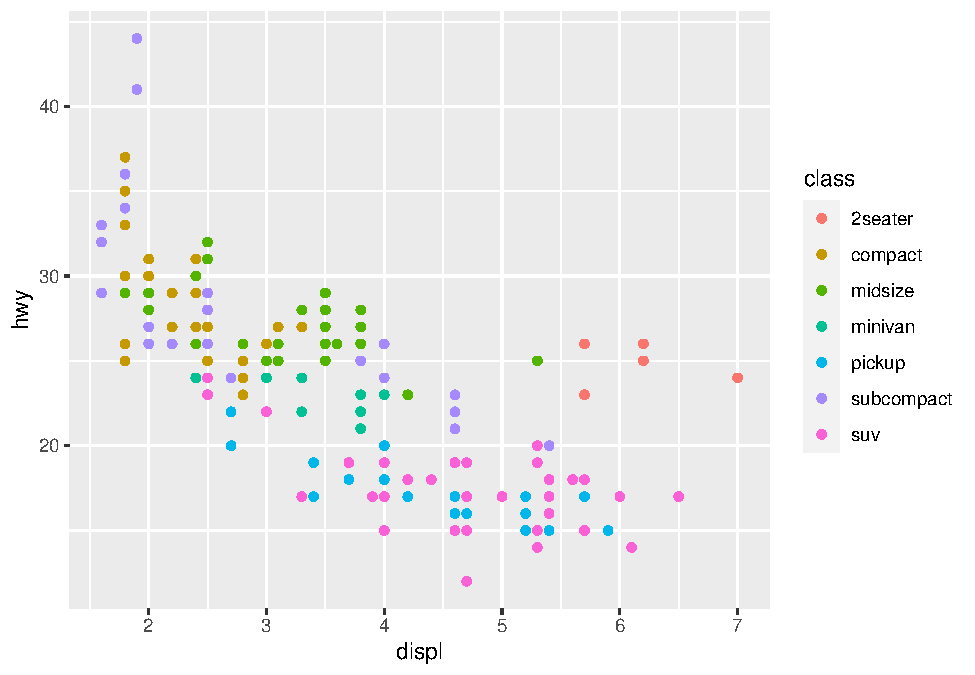
\includegraphics{R_learing_notes_files/figure-latex/unnamed-chunk-157-1} \end{center}

此外,如果我們映射 \texttt{color} 到一個邏輯條件,則如:

\begin{Shaded}
\begin{Highlighting}[]
\FunctionTok{ggplot}\NormalTok{(}\AttributeTok{data =}\NormalTok{ mpg) }\SpecialCharTok{+} \FunctionTok{geom\_point}\NormalTok{(}\AttributeTok{mapping =} \FunctionTok{aes}\NormalTok{(}\AttributeTok{x =}\NormalTok{ displ, }\AttributeTok{y =}\NormalTok{ hwy, }\AttributeTok{color =}\NormalTok{ displ }\SpecialCharTok{\textless{}} \DecValTok{5}\NormalTok{))}
\end{Highlighting}
\end{Shaded}

\begin{center}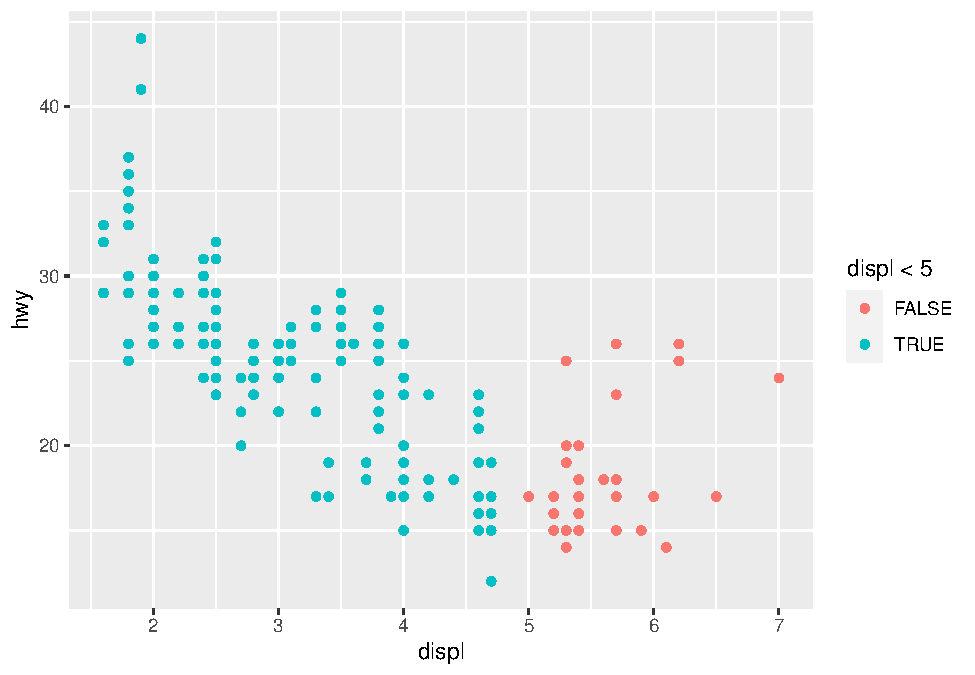
\includegraphics{R_learing_notes_files/figure-latex/unnamed-chunk-158-1} \end{center}

我們也可以使用 \texttt{size\ =\ class}。但要注意的是此時會出現 \texttt{Warning},因為把一個無序的變數 \texttt{class} 映射到一個有序的 aesthetic \texttt{size} 並不是一個好方法:

\begin{Shaded}
\begin{Highlighting}[]
\FunctionTok{ggplot}\NormalTok{(}\AttributeTok{data =}\NormalTok{ mpg) }\SpecialCharTok{+} \FunctionTok{geom\_point}\NormalTok{(}\AttributeTok{mapping =} \FunctionTok{aes}\NormalTok{(}\AttributeTok{x =}\NormalTok{ displ, }\AttributeTok{y =}\NormalTok{ hwy, }\AttributeTok{size =}\NormalTok{ class))}
\end{Highlighting}
\end{Shaded}

\begin{verbatim}
## Warning: Using size for a discrete variable is not advised.
\end{verbatim}

\begin{center}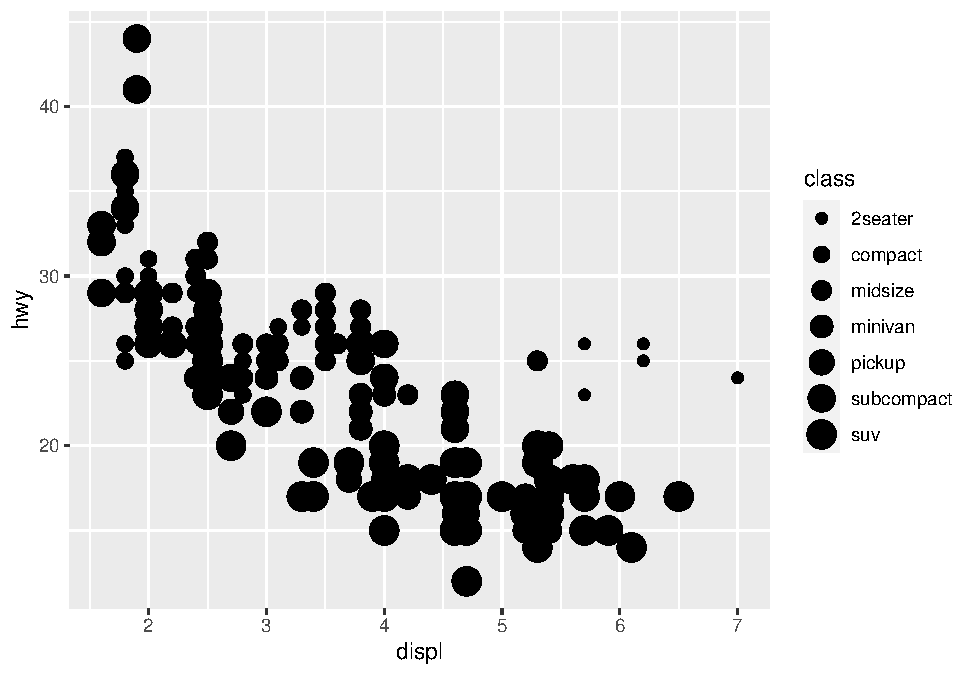
\includegraphics{R_learing_notes_files/figure-latex/unnamed-chunk-159-1} \end{center}

我們也可以映射 \texttt{class} 到 \texttt{alpha} 或 \texttt{shape},分別代表透明度與形狀,但也都會出現 \texttt{Warning}:

\begin{Shaded}
\begin{Highlighting}[]
\FunctionTok{ggplot}\NormalTok{(}\AttributeTok{data =}\NormalTok{ mpg) }\SpecialCharTok{+} \FunctionTok{geom\_point}\NormalTok{(}\AttributeTok{mapping =} \FunctionTok{aes}\NormalTok{(}\AttributeTok{x =}\NormalTok{ displ, }\AttributeTok{y =}\NormalTok{ hwy, }\AttributeTok{alpha =}\NormalTok{ class))}
\end{Highlighting}
\end{Shaded}

\begin{verbatim}
## Warning: Using alpha for a discrete variable is not advised.
\end{verbatim}

\begin{center}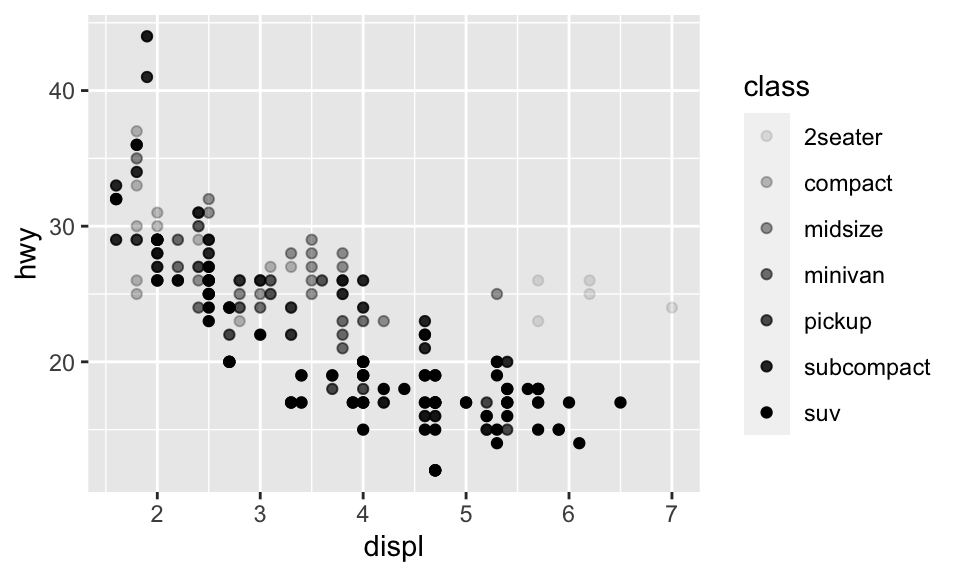
\includegraphics{R_learing_notes_files/figure-latex/unnamed-chunk-160-1} \end{center}

\begin{Shaded}
\begin{Highlighting}[]
\FunctionTok{ggplot}\NormalTok{(}\AttributeTok{data =}\NormalTok{ mpg) }\SpecialCharTok{+} \FunctionTok{geom\_point}\NormalTok{(}\AttributeTok{mapping =} \FunctionTok{aes}\NormalTok{(}\AttributeTok{x =}\NormalTok{ displ, }\AttributeTok{y =}\NormalTok{ hwy, }\AttributeTok{shape =}\NormalTok{ class))}
\end{Highlighting}
\end{Shaded}

\begin{verbatim}
## Warning: The shape palette can deal with a maximum of 6 discrete values because
## more than 6 becomes difficult to discriminate; you have 7. Consider
## specifying shapes manually if you must have them.
\end{verbatim}

\begin{verbatim}
## Warning: Removed 62 rows containing missing values (geom_point).
\end{verbatim}

\begin{center}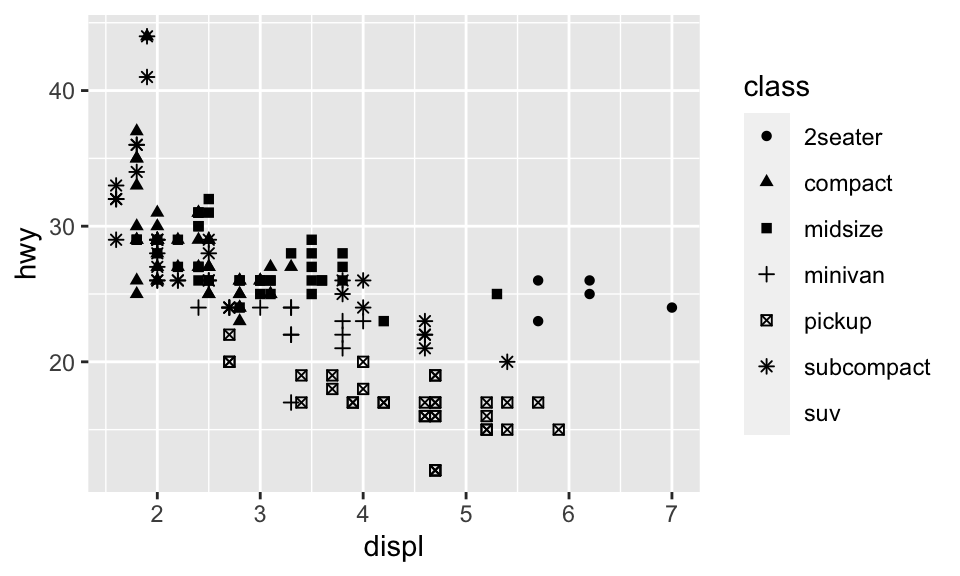
\includegraphics{R_learing_notes_files/figure-latex/unnamed-chunk-161-1} \end{center}

我們也可以從 \texttt{geom} 手動選擇 aesthetic properties,例如我們可以在 \texttt{geom()} 中加上 \texttt{color\ =\ "blue"},讓所有點都變成藍色:

\begin{Shaded}
\begin{Highlighting}[]
\FunctionTok{ggplot}\NormalTok{(}\AttributeTok{data =}\NormalTok{ mpg) }\SpecialCharTok{+} \FunctionTok{geom\_point}\NormalTok{(}\AttributeTok{mapping =} \FunctionTok{aes}\NormalTok{(}\AttributeTok{x =}\NormalTok{ displ, }\AttributeTok{y =}\NormalTok{ hwy), }\AttributeTok{color =} \StringTok{"blue"}\NormalTok{)}
\end{Highlighting}
\end{Shaded}

\begin{center}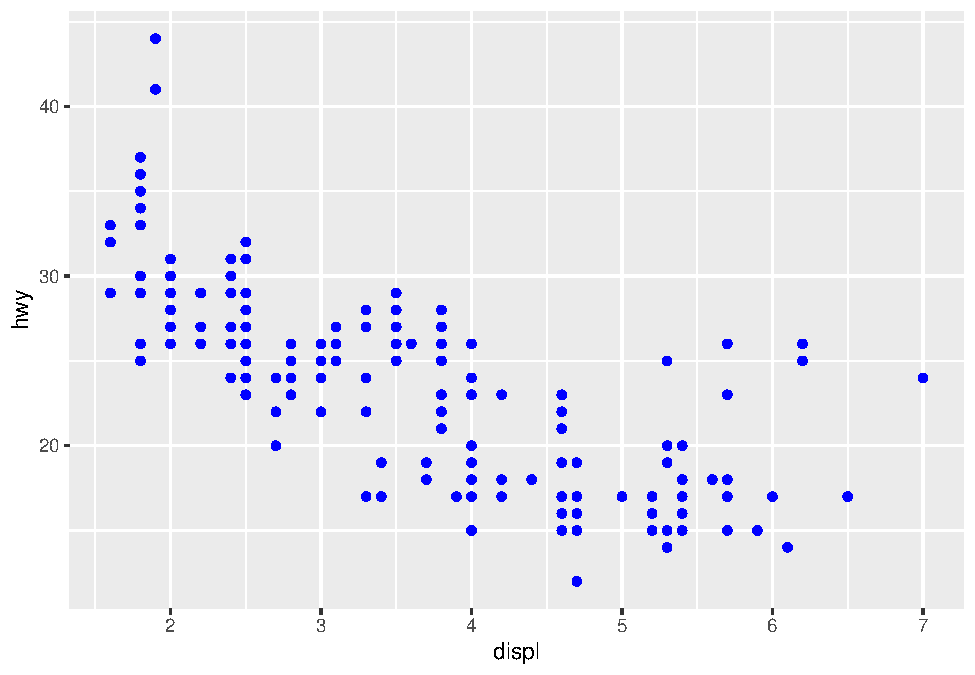
\includegraphics{R_learing_notes_files/figure-latex/unnamed-chunk-162-1} \end{center}

這樣的話,就只是改變顏色,顏色並未傳達更多資訊。不過,事實上 \texttt{ggplot2} 也可以手動設置 aesthetic,不過此處從略。

\hypertarget{facets}{%
\section{Facets}\label{facets}}

\begin{quote}
注意:類別變數才能繪製成 facets!
\end{quote}

除了把變數映射到 aesthetics,我們也可以把\textbf{類別變數}繪製成 facets,即分別繪製資料不同的子集。要繪製 facets,我們可以使用 \texttt{facet\_wrap()},其第一個引數是一個 formula,即 \texttt{\textasciitilde{}\ 變數名稱}。此外,也可以 \texttt{nrow} 或 \texttt{ncol} 來指定要有幾個 rows 或 columns。如我們要根據 \texttt{class} 來繪製 facets,而排成兩個 rows 的形式,即:

\begin{Shaded}
\begin{Highlighting}[]
\FunctionTok{ggplot}\NormalTok{(}\AttributeTok{data =}\NormalTok{ mpg) }\SpecialCharTok{+}
      \FunctionTok{geom\_point}\NormalTok{(}\AttributeTok{mapping =} \FunctionTok{aes}\NormalTok{(}\AttributeTok{x =}\NormalTok{ displ, }\AttributeTok{y =}\NormalTok{ hwy)) }\SpecialCharTok{+}
      \FunctionTok{facet\_wrap}\NormalTok{(}\SpecialCharTok{\textasciitilde{}}\NormalTok{ class, }\AttributeTok{nrow =} \DecValTok{2}\NormalTok{)}
\end{Highlighting}
\end{Shaded}

\begin{center}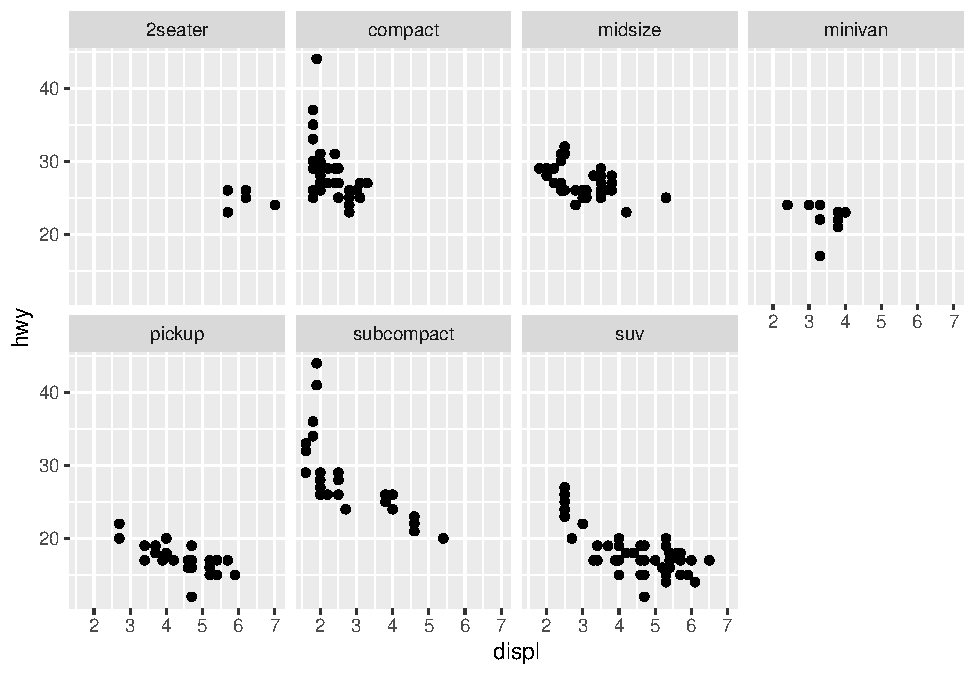
\includegraphics{R_learing_notes_files/figure-latex/unnamed-chunk-163-1} \end{center}

如果我們要把 facets 畫成兩個變數的組合,那就必須使用 \texttt{facet\_gird()},其語法如 \texttt{facet\_grid(row\ \textasciitilde{}\ col)}。以下的例子,因為 \texttt{drv} 共有三種值:\texttt{4}、\texttt{f}、\texttt{r},而 \texttt{cyl} 共有四種值:\texttt{4}、\texttt{5}、\texttt{6}、\texttt{8},所以:

\begin{Shaded}
\begin{Highlighting}[]
\FunctionTok{ggplot}\NormalTok{(}\AttributeTok{data =}\NormalTok{ mpg) }\SpecialCharTok{+}
      \FunctionTok{geom\_point}\NormalTok{(}\AttributeTok{mapping =} \FunctionTok{aes}\NormalTok{(}\AttributeTok{x =}\NormalTok{ displ, }\AttributeTok{y =}\NormalTok{ hwy)) }\SpecialCharTok{+}
      \FunctionTok{facet\_grid}\NormalTok{(drv }\SpecialCharTok{\textasciitilde{}}\NormalTok{ cyl)}
\end{Highlighting}
\end{Shaded}

\begin{center}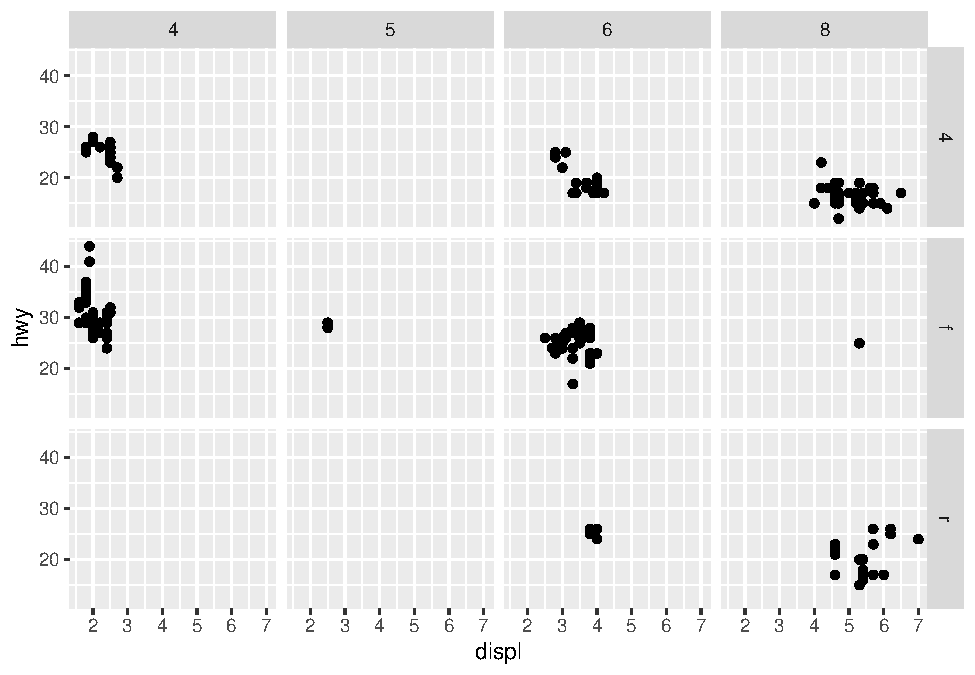
\includegraphics{R_learing_notes_files/figure-latex/unnamed-chunk-164-1} \end{center}

如果 row 或 column 其中一者不想要有變數,可以使用 \texttt{facet\_grid()}。

\hypertarget{ux5e7eux4f55ux7269ux4ef6}{%
\section{幾何物件}\label{ux5e7eux4f55ux7269ux4ef6}}

\emph{Geom} 是一種圖用來表示資料的幾何物件。例如,bar charts 使用 bar geoms,line charts 使用 line geoms,boxplots 使用 boxplot geoms 等。

要改變圖的 geom,即改變 \texttt{ggplot()} 所加的 geom function,例如我們把剛剛的 \texttt{geom\_point()} 改成 \texttt{geom\_smooth} 的話將會得到:

\begin{Shaded}
\begin{Highlighting}[]
\CommentTok{\# 對於 geom\_smooth() 中的 method 與 formula 用法可見其文檔}
\FunctionTok{ggplot}\NormalTok{(}\AttributeTok{data =}\NormalTok{ mpg) }\SpecialCharTok{+}
      \FunctionTok{geom\_smooth}\NormalTok{(}\AttributeTok{mapping =} \FunctionTok{aes}\NormalTok{(}\AttributeTok{x =}\NormalTok{ displ, }\AttributeTok{y =}\NormalTok{ hwy), }\AttributeTok{method =} \StringTok{\textquotesingle{}loess\textquotesingle{}}\NormalTok{, }\AttributeTok{formula =} \StringTok{\textquotesingle{}y \textasciitilde{} x\textquotesingle{}}\NormalTok{)}
\end{Highlighting}
\end{Shaded}

\begin{center}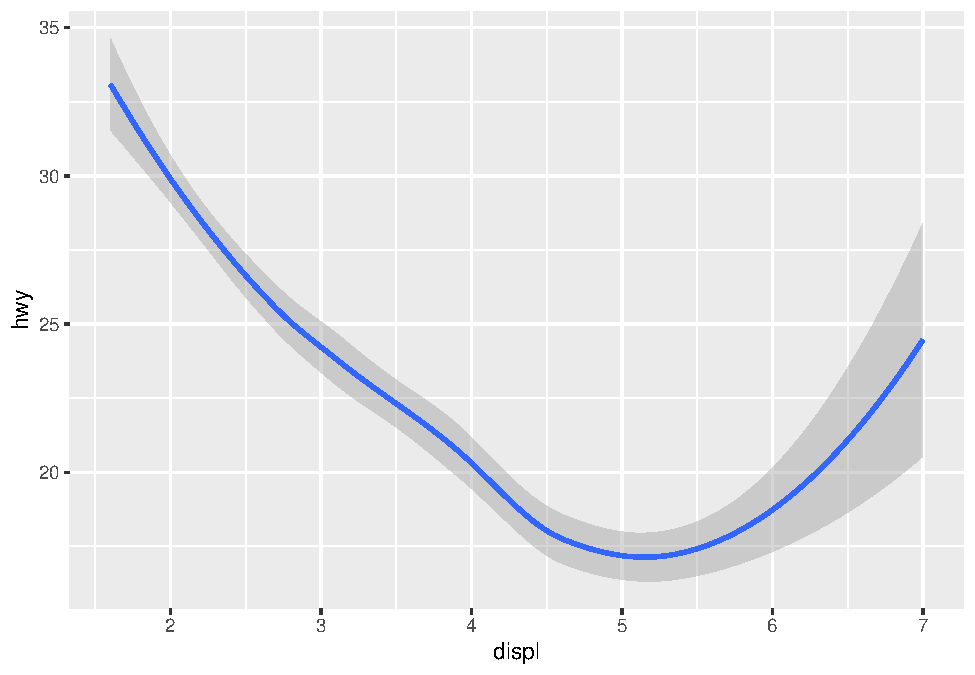
\includegraphics{R_learing_notes_files/figure-latex/unnamed-chunk-165-1} \end{center}

我們也可以設置 aesthetic。雖然不能設置線的 shape,但可以設定線的 linetype。例如,我們可以根據變數 \texttt{drv} 來繪製三條不同的線:

\begin{Shaded}
\begin{Highlighting}[]
\FunctionTok{ggplot}\NormalTok{(}\AttributeTok{data =}\NormalTok{ mpg) }\SpecialCharTok{+} 
  \FunctionTok{geom\_smooth}\NormalTok{(}\AttributeTok{mapping =} \FunctionTok{aes}\NormalTok{(}\AttributeTok{x =}\NormalTok{ displ, }\AttributeTok{y =}\NormalTok{ hwy, }\AttributeTok{linetype =}\NormalTok{ drv),}
              \AttributeTok{method =} \StringTok{"loess"}\NormalTok{, }\AttributeTok{formula =} \StringTok{"y \textasciitilde{} x"}\NormalTok{)}
\end{Highlighting}
\end{Shaded}

\begin{center}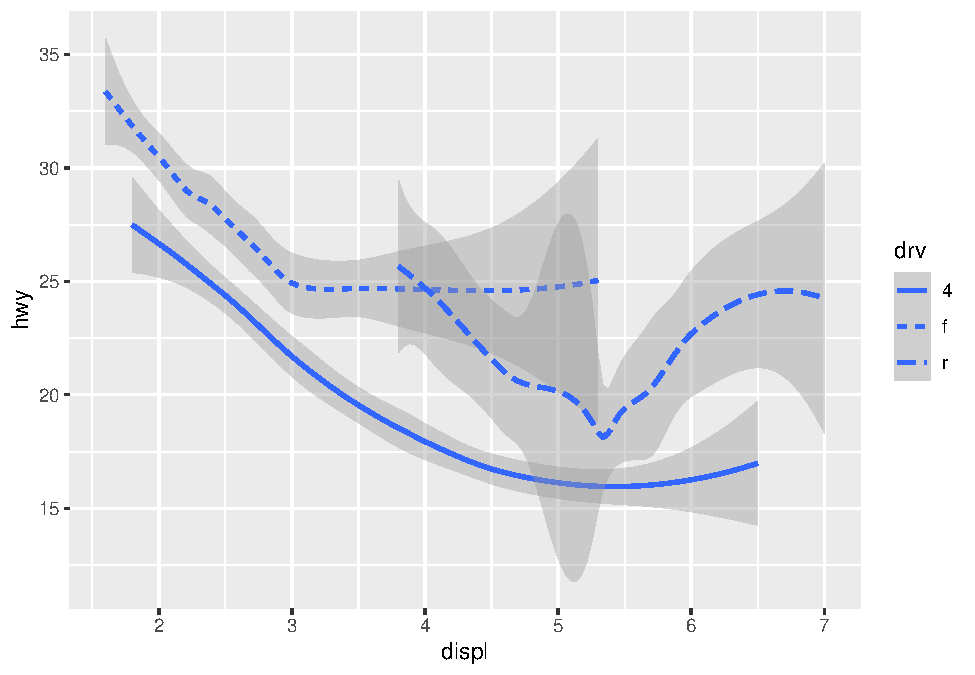
\includegraphics{R_learing_notes_files/figure-latex/unnamed-chunk-166-1} \end{center}

或者也可以疊加兩種 geom:

\begin{Shaded}
\begin{Highlighting}[]
\FunctionTok{ggplot}\NormalTok{(}\AttributeTok{data =}\NormalTok{ mpg) }\SpecialCharTok{+} 
  \FunctionTok{geom\_smooth}\NormalTok{(}\AttributeTok{mapping =} \FunctionTok{aes}\NormalTok{(}\AttributeTok{x =}\NormalTok{ displ, }\AttributeTok{y =}\NormalTok{ hwy, }\AttributeTok{color =}\NormalTok{ drv, }\AttributeTok{linetype =}\NormalTok{ drv),}
              \AttributeTok{method =} \StringTok{"loess"}\NormalTok{, }\AttributeTok{formula =} \StringTok{"y \textasciitilde{} x"}\NormalTok{) }\SpecialCharTok{+} 
  \FunctionTok{geom\_point}\NormalTok{(}\AttributeTok{mapping =} \FunctionTok{aes}\NormalTok{(}\AttributeTok{x =}\NormalTok{ displ, }\AttributeTok{y =}\NormalTok{ hwy, }\AttributeTok{color =}\NormalTok{ drv))}
\end{Highlighting}
\end{Shaded}

\begin{center}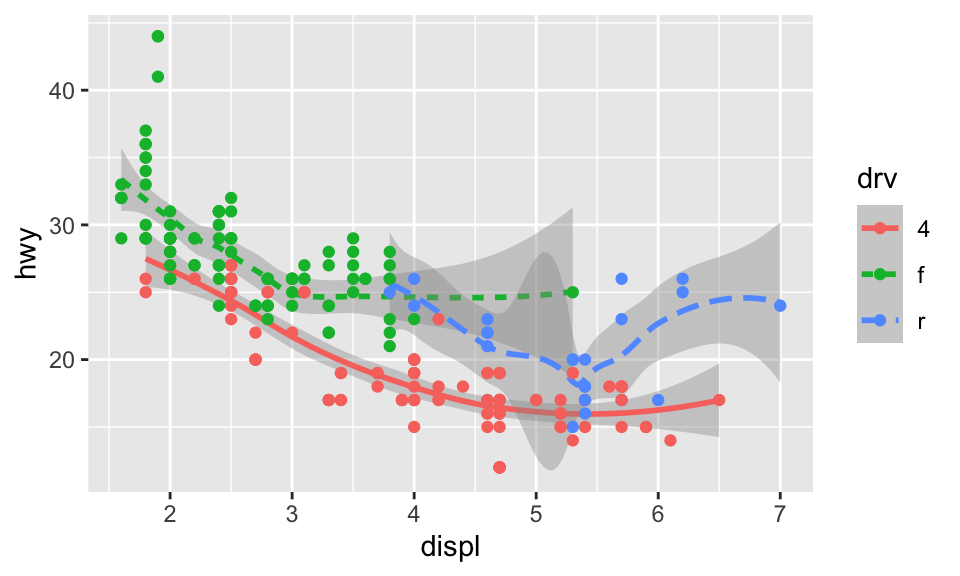
\includegraphics{R_learing_notes_files/figure-latex/unnamed-chunk-167-1} \end{center}

如果把引數放在 \texttt{ggplot()} 中,則會被視為 global mapping,將會套用到圖中的所有 geom;而放在 \texttt{geom()} 中則會被視為 local mapping,只會套用到該 geom。所以上述的程式碼也可以簡化為:

\begin{Shaded}
\begin{Highlighting}[]
\FunctionTok{ggplot}\NormalTok{(}\AttributeTok{data =}\NormalTok{ mpg, }\AttributeTok{mapping =} \FunctionTok{aes}\NormalTok{(}\AttributeTok{x =}\NormalTok{ displ, }\AttributeTok{y =}\NormalTok{ hwy, }\AttributeTok{color =}\NormalTok{ drv)) }\SpecialCharTok{+} 
  \FunctionTok{geom\_smooth}\NormalTok{(}\FunctionTok{aes}\NormalTok{(}\AttributeTok{linetype =}\NormalTok{ drv), }\AttributeTok{method =} \StringTok{"loess"}\NormalTok{, }\AttributeTok{formula =} \StringTok{"y \textasciitilde{} x"}\NormalTok{) }\SpecialCharTok{+} 
  \FunctionTok{geom\_point}\NormalTok{()}
\end{Highlighting}
\end{Shaded}

\begin{center}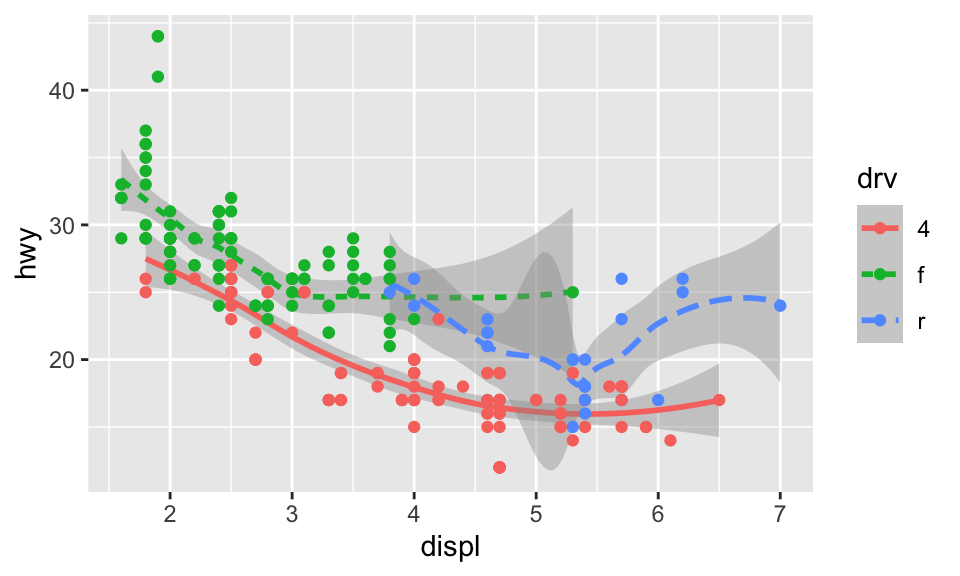
\includegraphics{R_learing_notes_files/figure-latex/unnamed-chunk-168-1} \end{center}

\hypertarget{ux7d71ux8a08ux8f49ux63db}{%
\section{統計轉換}\label{ux7d71ux8a08ux8f49ux63db}}

\texttt{diamonds} 是 \texttt{ggplot2} 中的一個 dataset,約有 54000 顆鑽石的資料,包含 \texttt{carat}、\texttt{cut}、\texttt{color}、\texttt{clarity}、\texttt{depth}、\texttt{table}、\texttt{price} 等變數。使用 \texttt{geom\_bar()} 可以依據某個變數畫出長條圖(bar chart),例如我們想要知道各種 cuts 到底有分別有多少鑽石,可以:

\begin{Shaded}
\begin{Highlighting}[]
\FunctionTok{ggplot}\NormalTok{(}\AttributeTok{data =}\NormalTok{ diamonds) }\SpecialCharTok{+} \FunctionTok{geom\_bar}\NormalTok{(}\AttributeTok{mapping =} \FunctionTok{aes}\NormalTok{(}\AttributeTok{x =}\NormalTok{ cut))}
\end{Highlighting}
\end{Shaded}

\begin{center}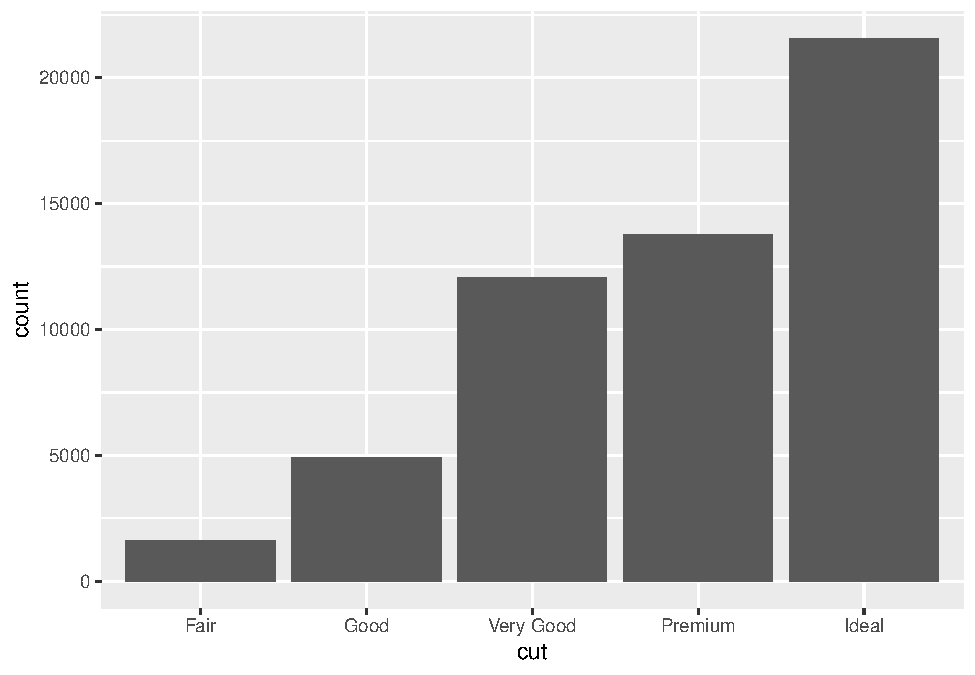
\includegraphics{R_learing_notes_files/figure-latex/unnamed-chunk-169-1} \end{center}

在此,\(x\) 軸為 \texttt{cut},是 \texttt{diamonds} 中的變數;\(y\) 軸為 \texttt{count},並非 \texttt{diamonds} 中的變數,而是自動計算在各個 \texttt{cut} 中鑽石的數量。某些圖會計算新的變數然,例如:

\begin{enumerate}
\def\labelenumi{\arabic{enumi}.}
\tightlist
\item
  長條圖、直方圖(histogram)或 frequency polygons 都會計算個數。
\item
  Smoothers 會適配模型然後畫出預測。
\item
  Boxplots 會計算分佈。
\end{enumerate}

用來計算新的值的演算法稱之為 \emph{stat},為 statistical transformation 的簡稱。例如以 \texttt{?geom\_bar} 查看 \texttt{geom\_bar()} 的幫助頁面,會發現其使用 \texttt{stat\_count()}。因為每個 geom 都有一個預設的 stat,反之亦然,所以我們可以把 geom 與 stat 交換使用。也因此,如果把上圖的 \texttt{geom\_bar()} 換成 \texttt{stat\_count()} 也會到相同的結果。

什麼時候需要明確地使用 stat 呢?

\begin{enumerate}
\def\labelenumi{\arabic{enumi}.}
\item
  想要替換預設的 stat 的時候。
\item
  想要換原本的 mapping 時。
\end{enumerate}

\begin{Shaded}
\begin{Highlighting}[]
\FunctionTok{ggplot}\NormalTok{(}\AttributeTok{data =}\NormalTok{ diamonds) }\SpecialCharTok{+}
  \FunctionTok{geom\_bar}\NormalTok{(}
    \AttributeTok{mapping =} \FunctionTok{aes}\NormalTok{(}\AttributeTok{x =}\NormalTok{ cut, }\AttributeTok{y =}\NormalTok{ ..prop.., }\AttributeTok{group =} \DecValTok{1}\NormalTok{)}
\NormalTok{  )}
\end{Highlighting}
\end{Shaded}

\begin{center}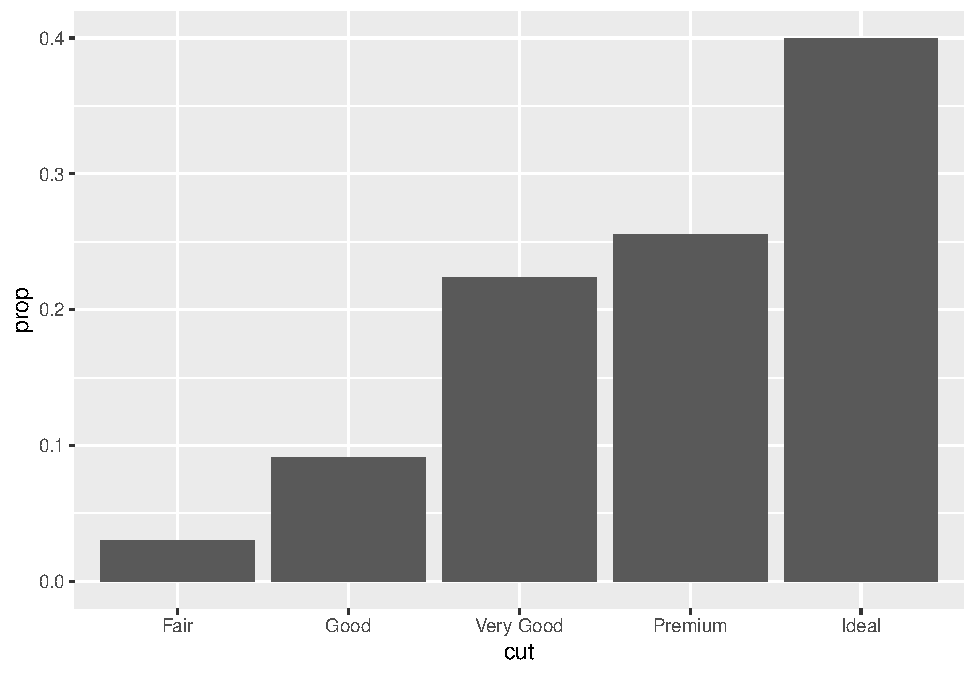
\includegraphics{R_learing_notes_files/figure-latex/unnamed-chunk-170-1} \end{center}

\begin{enumerate}
\def\labelenumi{\arabic{enumi}.}
\setcounter{enumi}{2}
\tightlist
\item
  想要使用其他的 statistical transformation 的時候。例如使用 \texttt{stat\_summary()},其會對每個 \texttt{x} 都 summarizes 其 \texttt{y}。
\end{enumerate}

\begin{Shaded}
\begin{Highlighting}[]
\FunctionTok{ggplot}\NormalTok{(}\AttributeTok{data =}\NormalTok{ diamonds) }\SpecialCharTok{+}
  \FunctionTok{stat\_summary}\NormalTok{(}
    \AttributeTok{mapping =} \FunctionTok{aes}\NormalTok{(}\AttributeTok{x =}\NormalTok{ cut, }\AttributeTok{y =}\NormalTok{ depth),}
    \AttributeTok{fun.min =}\NormalTok{ min,}
    \AttributeTok{fun.max =}\NormalTok{ max,}
    \AttributeTok{fun =}\NormalTok{ median}
\NormalTok{  )}
\end{Highlighting}
\end{Shaded}

\begin{center}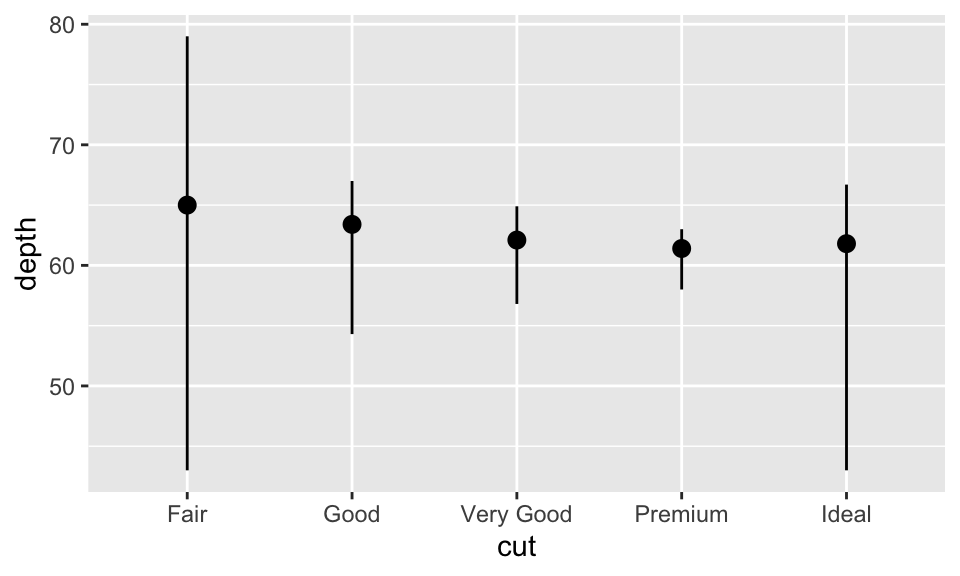
\includegraphics{R_learing_notes_files/figure-latex/unnamed-chunk-171-1} \end{center}

\hypertarget{position-adjustment}{%
\section{Position Adjustment}\label{position-adjustment}}

想要為長條圖著色,除了使用 \texttt{color},還可以使用 \texttt{fill},兩者的效果也不同:

\begin{Shaded}
\begin{Highlighting}[]
\FunctionTok{ggplot}\NormalTok{(}\AttributeTok{data =}\NormalTok{ diamonds) }\SpecialCharTok{+}
  \FunctionTok{geom\_bar}\NormalTok{(}\AttributeTok{mapping =} \FunctionTok{aes}\NormalTok{(}\AttributeTok{x =}\NormalTok{ cut, }\AttributeTok{color =}\NormalTok{ cut))}
\end{Highlighting}
\end{Shaded}

\begin{center}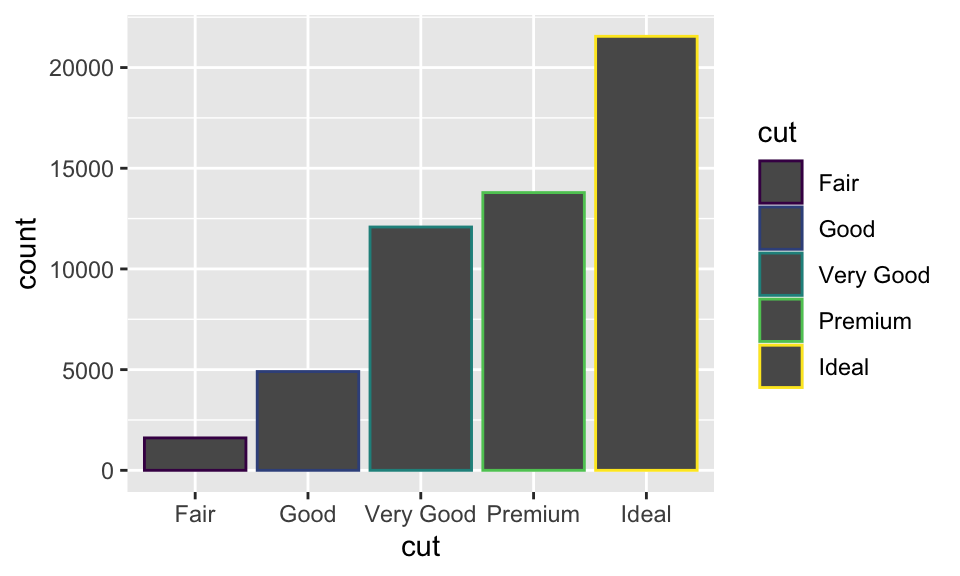
\includegraphics{R_learing_notes_files/figure-latex/unnamed-chunk-172-1} \end{center}

\begin{Shaded}
\begin{Highlighting}[]
\FunctionTok{ggplot}\NormalTok{(}\AttributeTok{data =}\NormalTok{ diamonds) }\SpecialCharTok{+}
  \FunctionTok{geom\_bar}\NormalTok{(}\AttributeTok{mapping =} \FunctionTok{aes}\NormalTok{(}\AttributeTok{x =}\NormalTok{ cut, }\AttributeTok{fill =}\NormalTok{ cut))}
\end{Highlighting}
\end{Shaded}

\begin{center}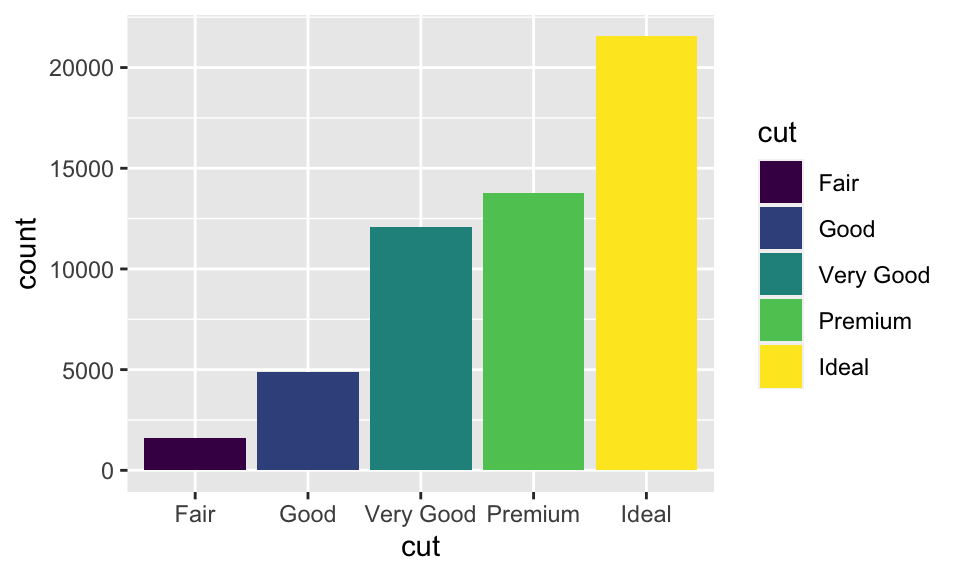
\includegraphics{R_learing_notes_files/figure-latex/unnamed-chunk-172-2} \end{center}

如果 \texttt{fill} 指定為另一個變數的話,就會自動變成「堆疊」的形式,如:

\begin{Shaded}
\begin{Highlighting}[]
\FunctionTok{ggplot}\NormalTok{(}\AttributeTok{data =}\NormalTok{ diamonds, }\AttributeTok{mapping =} \FunctionTok{aes}\NormalTok{(}\AttributeTok{x =}\NormalTok{ cut, }\AttributeTok{fill =}\NormalTok{ clarity)) }\SpecialCharTok{+} 
  \FunctionTok{geom\_bar}\NormalTok{()}
\end{Highlighting}
\end{Shaded}

\begin{center}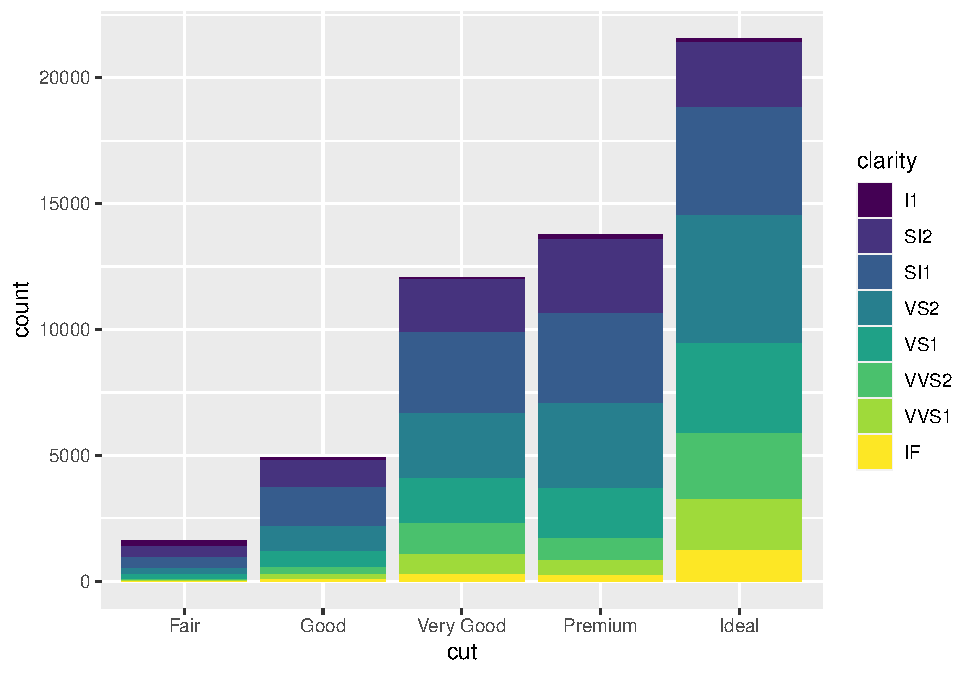
\includegraphics{R_learing_notes_files/figure-latex/unnamed-chunk-173-1} \end{center}

這種堆疊是透過位置調整(position adjustment)進行的。\texttt{position} 預設為 \texttt{position="stack"},而我們還能把 \texttt{position} 指定成其他三種選項:\texttt{identity}、\texttt{dodge} 與 \texttt{fill}:

\begin{enumerate}
\def\labelenumi{\arabic{enumi}.}
\tightlist
\item
  \texttt{position\ =\ "identity"}:用在 bar chart 上效果有點像 \texttt{stack},但差別在調整透明度後可以看出來(即 \texttt{alpha\ =\ 1/5});雖然還是不明顯,但差別在 \texttt{identity} 的各個物件是會相互堆疊的。例如在下圖中,調整透明度明明應該所有物件的透明度都相同,但越靠下的部分透明度顯然越低,這就是因為越靠下的部分有越多個物件重疊在一起,使得圖形顯得較不透明。
\end{enumerate}

\begin{Shaded}
\begin{Highlighting}[]
\FunctionTok{ggplot}\NormalTok{(}\AttributeTok{data =}\NormalTok{ diamonds, }\AttributeTok{mapping =} \FunctionTok{aes}\NormalTok{(}\AttributeTok{x =}\NormalTok{ cut, }\AttributeTok{fill =}\NormalTok{ clarity)) }\SpecialCharTok{+}
  \FunctionTok{geom\_bar}\NormalTok{(}\AttributeTok{alpha =} \DecValTok{1}\SpecialCharTok{/}\DecValTok{5}\NormalTok{, }\AttributeTok{position =} \StringTok{"identity"}\NormalTok{)}
\end{Highlighting}
\end{Shaded}

\begin{center}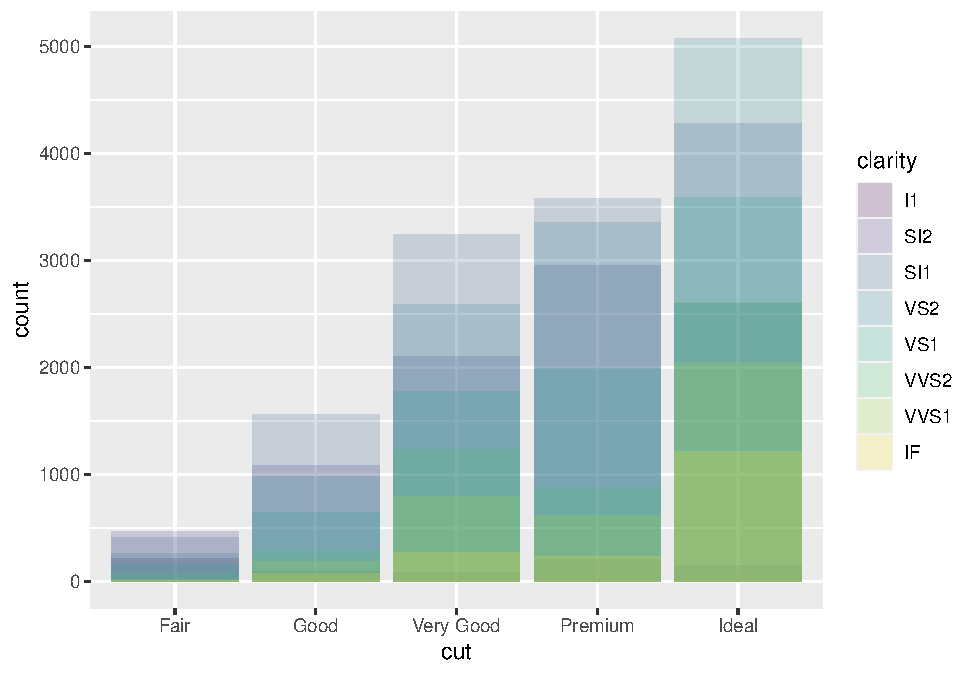
\includegraphics{R_learing_notes_files/figure-latex/unnamed-chunk-174-1} \end{center}

\begin{enumerate}
\def\labelenumi{\arabic{enumi}.}
\setcounter{enumi}{1}
\tightlist
\item
  \texttt{position\ =\ "fill"}:依據指定的變數(此數為 \texttt{clarity})堆疊,差別在高度相同,所以便於我們比較組間的比例差別。
\end{enumerate}

\begin{Shaded}
\begin{Highlighting}[]
\FunctionTok{ggplot}\NormalTok{(}\AttributeTok{data =}\NormalTok{ diamonds, }\AttributeTok{mapping =} \FunctionTok{aes}\NormalTok{(}\AttributeTok{x =}\NormalTok{ cut, }\AttributeTok{fill =}\NormalTok{ clarity)) }\SpecialCharTok{+}
  \FunctionTok{geom\_bar}\NormalTok{(}\AttributeTok{position =} \StringTok{"fill"}\NormalTok{)}
\end{Highlighting}
\end{Shaded}

\begin{center}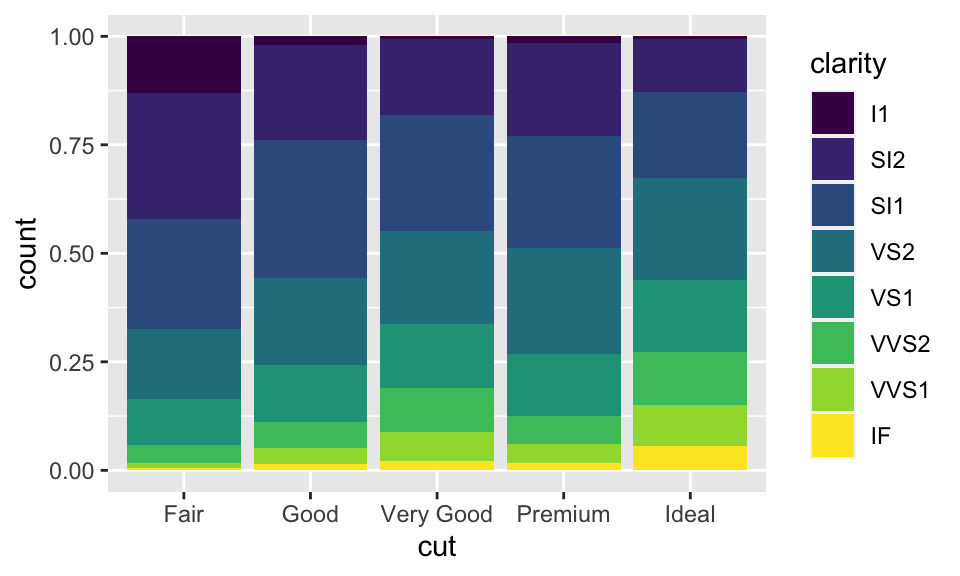
\includegraphics{R_learing_notes_files/figure-latex/unnamed-chunk-175-1} \end{center}

\begin{enumerate}
\def\labelenumi{\arabic{enumi}.}
\setcounter{enumi}{2}
\tightlist
\item
  \texttt{position\ =\ "dodge"}:以此例而言,即是對於每個不同的 \texttt{cut},都分別把其各個 \texttt{clarity} 展現在逐一呈現,而非用堆疊的方式。
\end{enumerate}

\begin{Shaded}
\begin{Highlighting}[]
\FunctionTok{ggplot}\NormalTok{(}\AttributeTok{data =}\NormalTok{ diamonds, }\AttributeTok{mapping =} \FunctionTok{aes}\NormalTok{(}\AttributeTok{x =}\NormalTok{ cut, }\AttributeTok{fill =}\NormalTok{ clarity)) }\SpecialCharTok{+}
  \FunctionTok{geom\_bar}\NormalTok{(}\AttributeTok{position =} \StringTok{"dodge"}\NormalTok{)}
\end{Highlighting}
\end{Shaded}

\begin{center}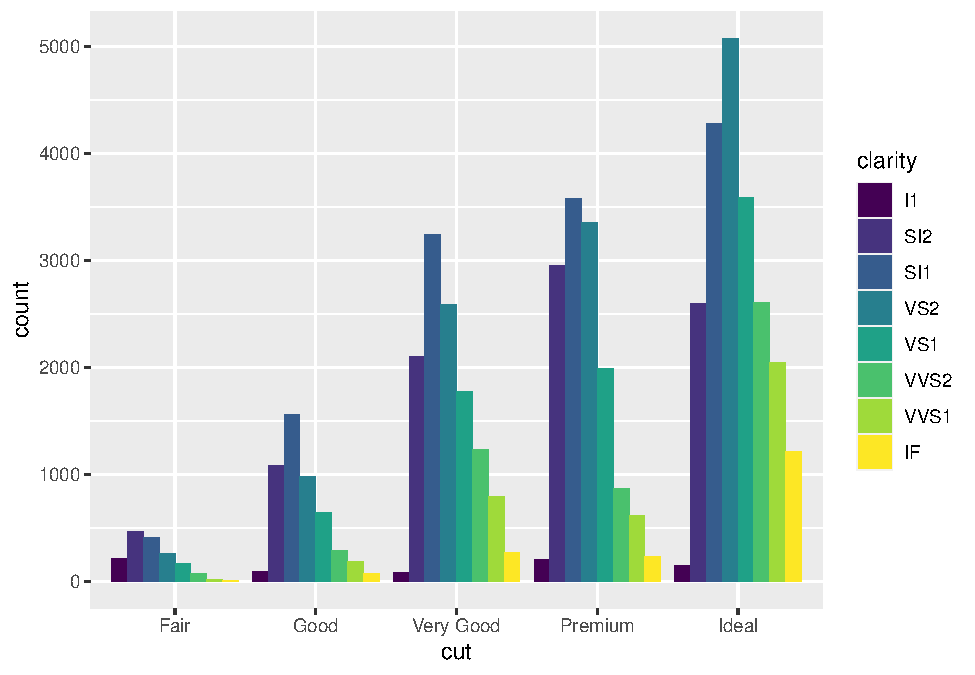
\includegraphics{R_learing_notes_files/figure-latex/unnamed-chunk-176-1} \end{center}

此外,當然還有其他 \texttt{position} 的引數可用,例如 \texttt{position\ =\ "jitter"},其在 bar chart 中沒什麼用,但在散佈圖中有大用。回憶節 \ref{create} 的散佈圖:

\begin{Shaded}
\begin{Highlighting}[]
\FunctionTok{ggplot}\NormalTok{(}\AttributeTok{data =}\NormalTok{ mpg) }\SpecialCharTok{+} \FunctionTok{geom\_point}\NormalTok{(}\AttributeTok{mapping =} \FunctionTok{aes}\NormalTok{(}\AttributeTok{x =}\NormalTok{ displ, }\AttributeTok{y =}\NormalTok{ hwy))}
\end{Highlighting}
\end{Shaded}

\begin{center}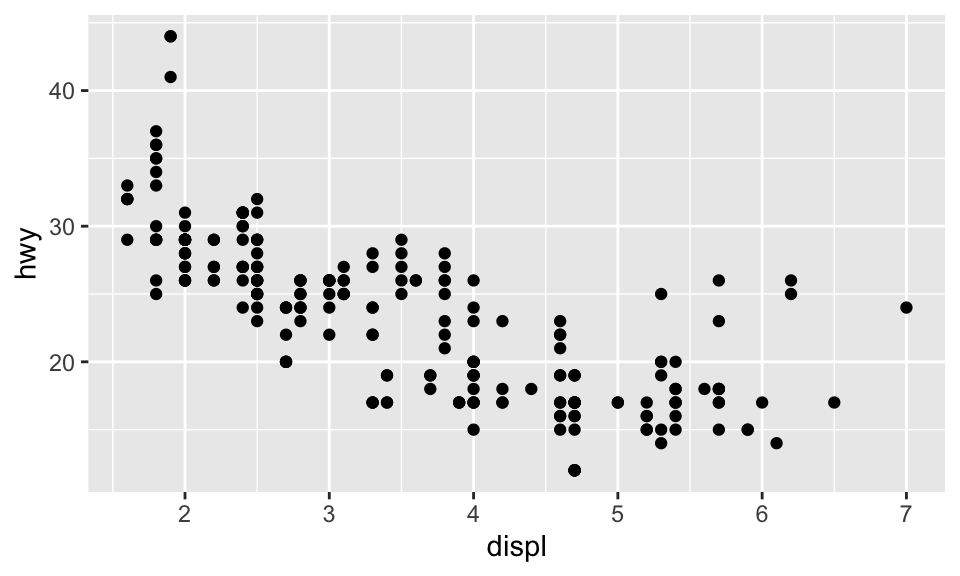
\includegraphics{R_learing_notes_files/figure-latex/unnamed-chunk-177-1} \end{center}

事實上,\texttt{mpg} 明明有 234 個觀察值,如:

\begin{Shaded}
\begin{Highlighting}[]
\FunctionTok{str}\NormalTok{(mpg)}
\CommentTok{\# tibble [234 × 11] (S3: tbl\_df/tbl/data.frame)}
\CommentTok{\# ...}
\end{Highlighting}
\end{Shaded}

但上面的散佈圖卻只有顯示 126 個點,為什麼?因為 \textbf{overplotting}!有些點的座標相同,所以相互覆蓋了。設置 \texttt{position\ =\ "jitter"} 可以解決這個問題,這會在每個點加入一點點 random noise,排除 overplotting 的問題。

\begin{Shaded}
\begin{Highlighting}[]
\FunctionTok{ggplot}\NormalTok{(}\AttributeTok{data =}\NormalTok{ mpg, }\AttributeTok{mapping =} \FunctionTok{aes}\NormalTok{(}\AttributeTok{x =}\NormalTok{ displ, }\AttributeTok{y =}\NormalTok{ hwy)) }\SpecialCharTok{+} 
  \FunctionTok{geom\_point}\NormalTok{(}\AttributeTok{position =} \StringTok{"jitter"}\NormalTok{)}
\end{Highlighting}
\end{Shaded}

\begin{center}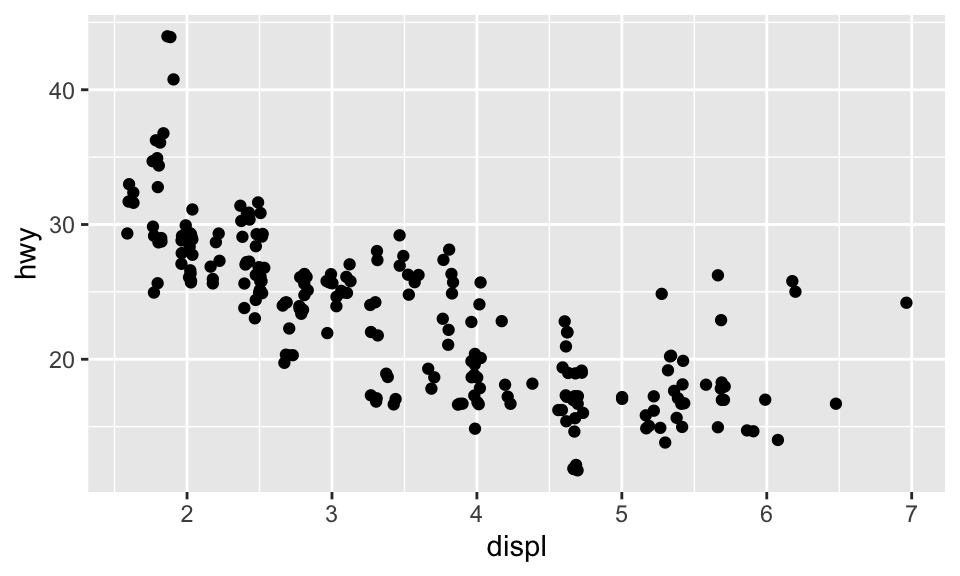
\includegraphics{R_learing_notes_files/figure-latex/unnamed-chunk-179-1} \end{center}

\hypertarget{ux5ea7ux6a19ux7cfbux7d71}{%
\section{座標系統}\label{ux5ea7ux6a19ux7cfbux7d71}}

除了前面使用的笛卡兒座標系統,還有其他有用的座標系統:

\begin{enumerate}
\def\labelenumi{\arabic{enumi}.}
\tightlist
\item
  \texttt{coord\_flip()}:繪製旋轉 90 度的直角坐標,如:
\end{enumerate}

\begin{Shaded}
\begin{Highlighting}[]
\FunctionTok{ggplot}\NormalTok{(}\AttributeTok{data =}\NormalTok{ mpg, }\AttributeTok{mapping =} \FunctionTok{aes}\NormalTok{(}\AttributeTok{x =}\NormalTok{ class, }\AttributeTok{y =}\NormalTok{ hwy)) }\SpecialCharTok{+} \FunctionTok{geom\_boxplot}\NormalTok{()}
\end{Highlighting}
\end{Shaded}

\begin{center}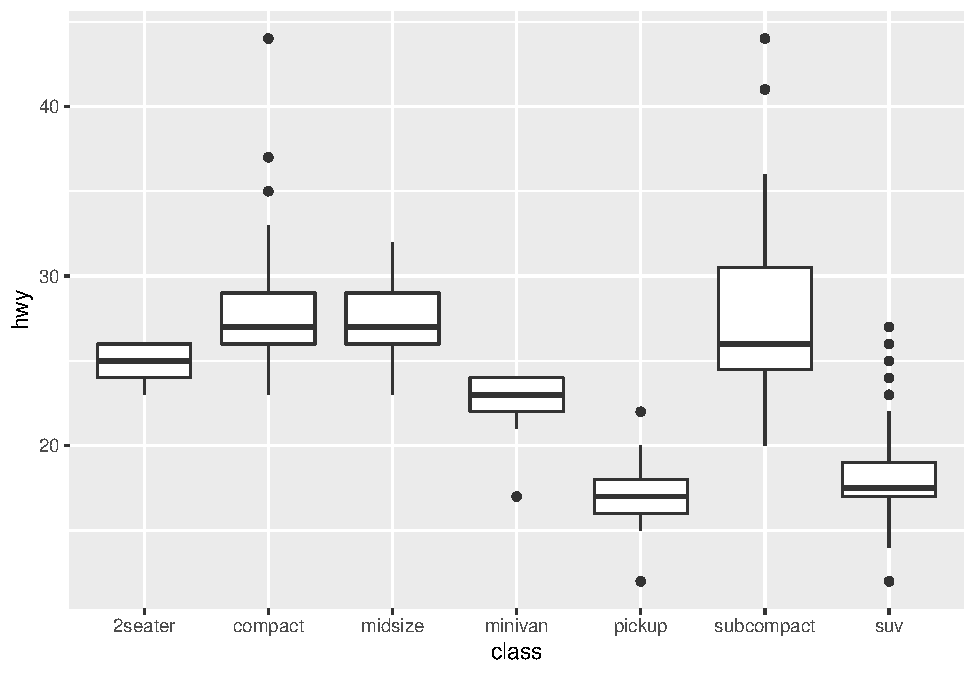
\includegraphics{R_learing_notes_files/figure-latex/unnamed-chunk-180-1} \end{center}

\begin{Shaded}
\begin{Highlighting}[]
\FunctionTok{ggplot}\NormalTok{(}\AttributeTok{data =}\NormalTok{ mpg, }\AttributeTok{mapping =} \FunctionTok{aes}\NormalTok{(}\AttributeTok{x =}\NormalTok{ class, }\AttributeTok{y =}\NormalTok{ hwy)) }\SpecialCharTok{+} \FunctionTok{geom\_boxplot}\NormalTok{() }\SpecialCharTok{+} \FunctionTok{coord\_flip}\NormalTok{()}
\end{Highlighting}
\end{Shaded}

\begin{center}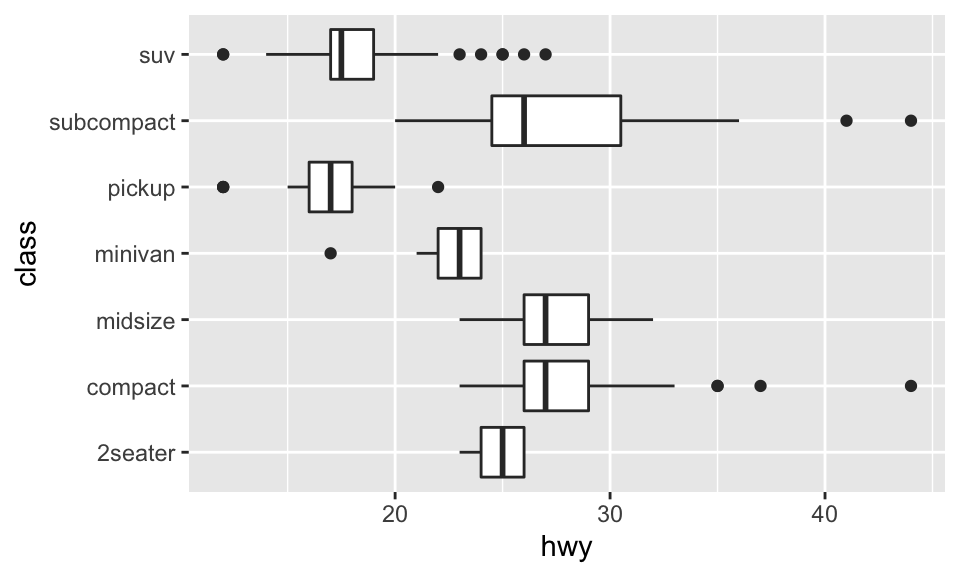
\includegraphics{R_learing_notes_files/figure-latex/unnamed-chunk-180-2} \end{center}

\begin{enumerate}
\def\labelenumi{\arabic{enumi}.}
\setcounter{enumi}{1}
\tightlist
\item
  \texttt{coord\_quickmap()}:繪製有正確方位比例的地圖\footnote{另有 \texttt{coord\_map()},功能與 \texttt{coord\_quickmap()} 類似。\texttt{coord\_map()} 預設使用\href{https://zh.wikipedia.org/wiki/\%E9\%BA\%A5\%E5\%8D\%A1\%E6\%89\%98\%E6\%8A\%95\%E5\%BD\%B1\%E6\%B3\%95}{麥卡托投影法(Mercator projection)}。而兩者的差別在 \texttt{coord\_quickmap} 為 \texttt{coord\_map()} 的近似,忽略了地球在不同經緯度比例的曲度差異,因此運行速率較快,但也稍微不準確。},如:
\end{enumerate}

\begin{Shaded}
\begin{Highlighting}[]
\NormalTok{nz }\OtherTok{\textless{}{-}} \FunctionTok{map\_data}\NormalTok{(}\StringTok{"nz"}\NormalTok{)}

\FunctionTok{ggplot}\NormalTok{(nz, }\FunctionTok{aes}\NormalTok{(long, lat, }\AttributeTok{group =}\NormalTok{ group)) }\SpecialCharTok{+} 
  \FunctionTok{geom\_polygon}\NormalTok{(}\AttributeTok{fill =} \StringTok{"white"}\NormalTok{, }\AttributeTok{color =} \StringTok{"black"}\NormalTok{)}
\end{Highlighting}
\end{Shaded}

\begin{center}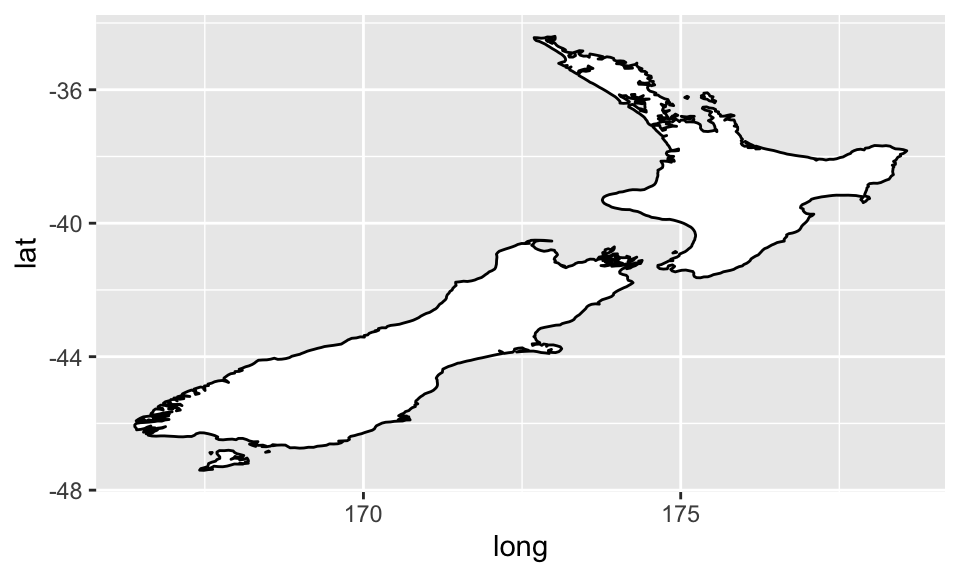
\includegraphics{R_learing_notes_files/figure-latex/unnamed-chunk-181-1} \end{center}

\begin{Shaded}
\begin{Highlighting}[]
\FunctionTok{ggplot}\NormalTok{(nz, }\FunctionTok{aes}\NormalTok{(long, lat, }\AttributeTok{group =}\NormalTok{ group)) }\SpecialCharTok{+} 
  \FunctionTok{geom\_polygon}\NormalTok{(}\AttributeTok{fill =} \StringTok{"white"}\NormalTok{, }\AttributeTok{color =} \StringTok{"black"}\NormalTok{) }\SpecialCharTok{+} \FunctionTok{coord\_quickmap}\NormalTok{()}
\end{Highlighting}
\end{Shaded}

\begin{center}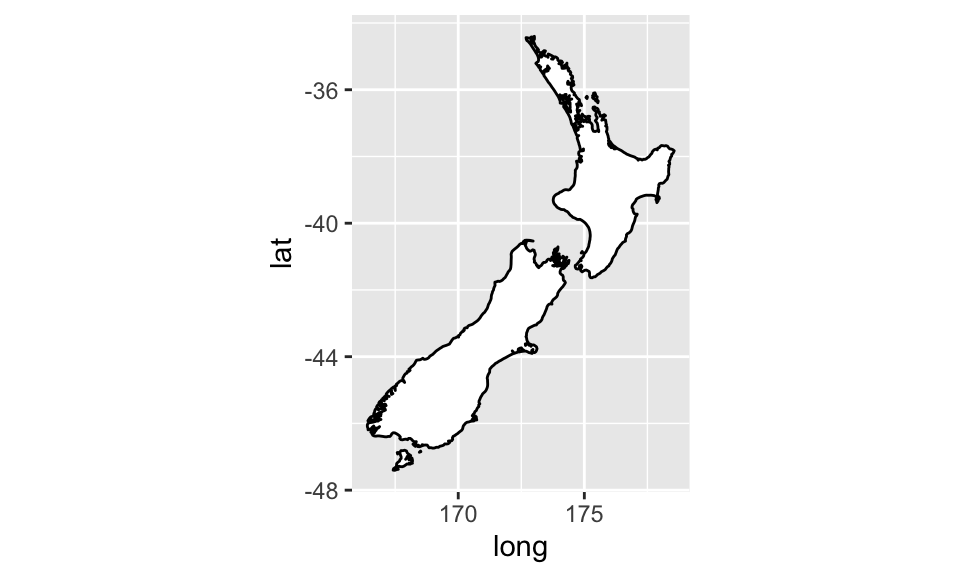
\includegraphics{R_learing_notes_files/figure-latex/unnamed-chunk-181-2} \end{center}

\begin{enumerate}
\def\labelenumi{\arabic{enumi}.}
\setcounter{enumi}{2}
\tightlist
\item
  \texttt{coord\_polar()}:繪製極座標圖(polar coordinates),結合 bar char 與 Coxcomb chart,如:
\end{enumerate}

\begin{Shaded}
\begin{Highlighting}[]
\NormalTok{bar }\OtherTok{\textless{}{-}} \FunctionTok{ggplot}\NormalTok{(}\AttributeTok{data =}\NormalTok{ diamonds) }\SpecialCharTok{+}
  \FunctionTok{geom\_bar}\NormalTok{(}\AttributeTok{mapping =} \FunctionTok{aes}\NormalTok{(}\AttributeTok{x =}\NormalTok{ cut, }\AttributeTok{fill =}\NormalTok{ cut), }\AttributeTok{show.legend =} \ConstantTok{FALSE}\NormalTok{, }\AttributeTok{width =} \DecValTok{1}\NormalTok{) }\SpecialCharTok{+}
  \FunctionTok{theme}\NormalTok{(}\AttributeTok{aspect.ratio =} \DecValTok{1}\NormalTok{) }\SpecialCharTok{+} \FunctionTok{labs}\NormalTok{(}\AttributeTok{x =} \ConstantTok{NULL}\NormalTok{, }\AttributeTok{y =} \ConstantTok{NULL}\NormalTok{)}

\NormalTok{bar }\SpecialCharTok{+} \FunctionTok{coord\_polar}\NormalTok{()}
\end{Highlighting}
\end{Shaded}

\begin{center}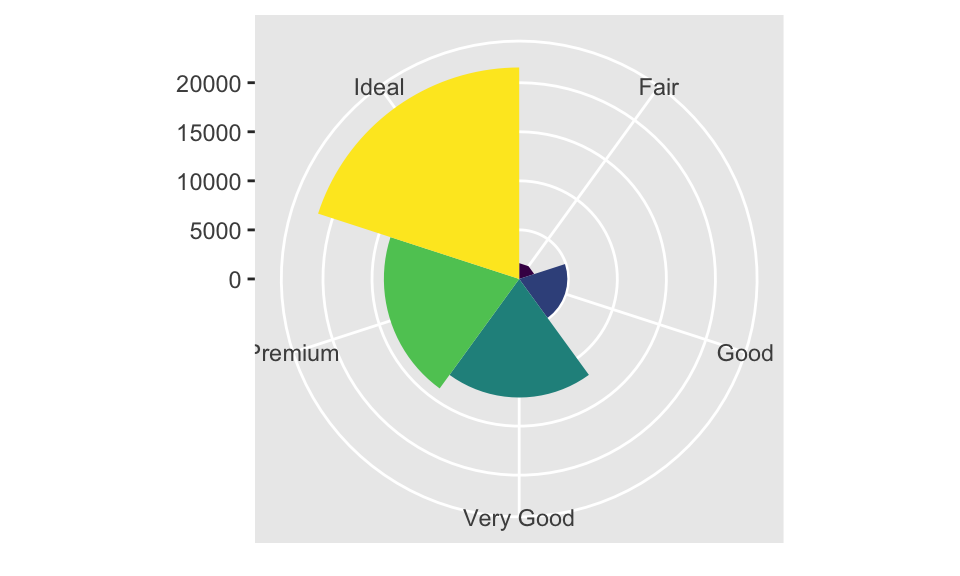
\includegraphics{R_learing_notes_files/figure-latex/unnamed-chunk-182-1} \end{center}

\begin{enumerate}
\def\labelenumi{\arabic{enumi}.}
\setcounter{enumi}{3}
\tightlist
\item
  \texttt{coord\_fixed}:因為人對與 45 度線的差異感受最明顯,而 \texttt{coord\_fixed()} 可以讓 \texttt{geom\_abline()}(用以產生 reference lines 的 geom)產生的線為 45 度,如:
\end{enumerate}

\begin{Shaded}
\begin{Highlighting}[]
\NormalTok{p }\OtherTok{\textless{}{-}} \FunctionTok{ggplot}\NormalTok{(}\AttributeTok{data =}\NormalTok{ mpg, }\AttributeTok{mapping =} \FunctionTok{aes}\NormalTok{(}\AttributeTok{x =}\NormalTok{ cty, }\AttributeTok{y =}\NormalTok{ hwy)) }\SpecialCharTok{+}
  \FunctionTok{geom\_point}\NormalTok{() }\SpecialCharTok{+} \FunctionTok{geom\_abline}\NormalTok{()}

\NormalTok{p }\SpecialCharTok{+} \FunctionTok{coord\_fixed}\NormalTok{()  }\CommentTok{\# 如果不加 coord\_fixed(),比例將會跑掉。}
\end{Highlighting}
\end{Shaded}

\begin{center}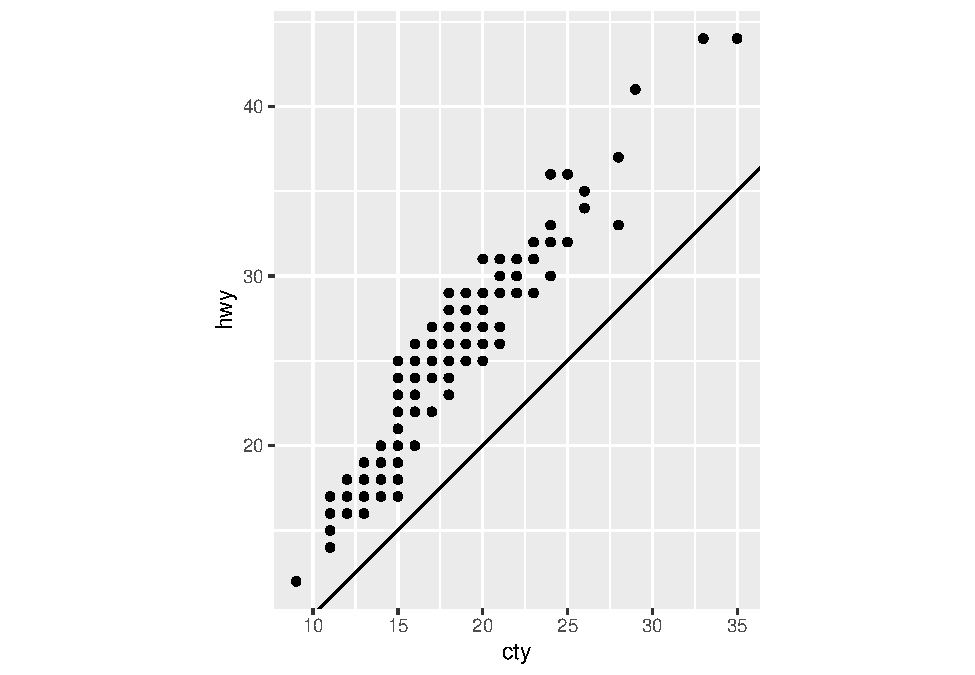
\includegraphics{R_learing_notes_files/figure-latex/unnamed-chunk-183-1} \end{center}

\hypertarget{ux6a19ux7c64-1}{%
\section{標籤}\label{ux6a19ux7c64-1}}

\texttt{labs()} 能使我們為圖加上標題、註解或更改 \texttt{x} 軸、\texttt{y} 軸的名稱,如:

\begin{Shaded}
\begin{Highlighting}[]
\FunctionTok{ggplot}\NormalTok{(}\AttributeTok{data =}\NormalTok{ mpg, }\AttributeTok{mapping =} \FunctionTok{aes}\NormalTok{(}\AttributeTok{x =}\NormalTok{ class, }\AttributeTok{y =}\NormalTok{ hwy)) }\SpecialCharTok{+} 
  \FunctionTok{geom\_boxplot}\NormalTok{() }\SpecialCharTok{+} 
  \FunctionTok{coord\_flip}\NormalTok{() }\SpecialCharTok{+}
  \FunctionTok{labs}\NormalTok{(}\AttributeTok{y =} \StringTok{"Highway MPG"}\NormalTok{,}
       \AttributeTok{x =} \StringTok{"Class"}\NormalTok{,}
       \AttributeTok{title =} \StringTok{"Highway MPG by car class"}\NormalTok{,}
       \AttributeTok{subtitle =} \StringTok{"1999{-}2008"}\NormalTok{,}
       \AttributeTok{caption =} \StringTok{"Source: http://fueleconomy.gov"}\NormalTok{)}
\end{Highlighting}
\end{Shaded}

\begin{center}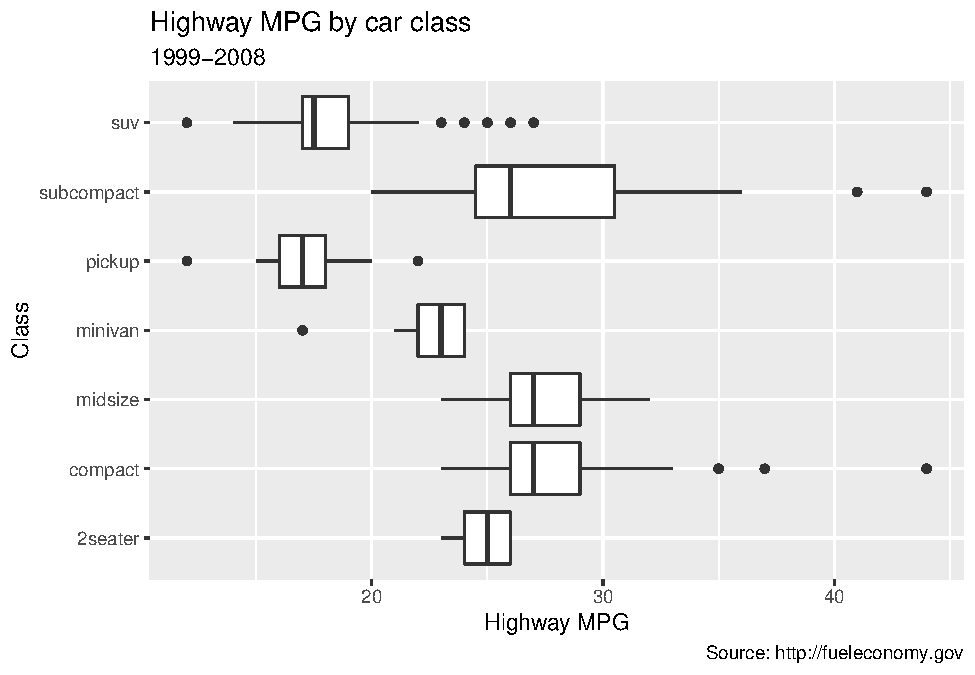
\includegraphics{R_learing_notes_files/figure-latex/unnamed-chunk-184-1} \end{center}

\hypertarget{dplyr}{%
\chapter{\texorpdfstring{以 \texttt{dplyr} 轉換資料}{以 dplyr 轉換資料}}\label{dplyr}}

\hypertarget{ux524dux8a00}{%
\section{前言}\label{ux524dux8a00}}

一拿到資料,除了以視覺化的方式快速洞察資料的樣貌,我們可能還需要:

\begin{enumerate}
\def\labelenumi{\arabic{enumi}.}
\item
  新增新的變數。
\item
  統整。
\item
  重新命名變數。
\item
  重新排列觀察值的順序。
\end{enumerate}

\texttt{dplyr} 的某些功能也能以 \texttt{data.table} 完成,並且兩者各有所長(\texttt{data.table} 的介紹可見節 \ref{datatable}),而本章將要介紹 \texttt{dplyr},為 \texttt{tidyverse} 中一個重要的成員,用以資料轉換。本章的任務是以 \texttt{nycflights13} 資料為例,簡介 \texttt{dplyr} 的使用。

\hypertarget{ux524dux7f6eux4f5cux696d-1}{%
\subsection{前置作業}\label{ux524dux7f6eux4f5cux696d-1}}

先載入 \texttt{nycflights13} 與 \texttt{tidyverse}:

\begin{Shaded}
\begin{Highlighting}[]
\FunctionTok{library}\NormalTok{(nycflights13)}
\FunctionTok{library}\NormalTok{(tidyverse)}
\end{Highlighting}
\end{Shaded}

要注意的是,\texttt{dplyr} 與 base R 一套件 \texttt{stats} 的某些函數名稱相同,如 \texttt{filter} 與 \texttt{lag}。如果是先載入 \texttt{stats},後載入 \texttt{dplyr} 的話,則使用 \texttt{filter()} 將會是 \texttt{dplyr} 的 \texttt{filter},這時候如果還想使用 \texttt{stats} 的 \texttt{filter()},則需使用其全名,即 \texttt{stats::filter()}。反之,如果是先載入 \texttt{dplyr},後載入 \texttt{stats},則使用 \texttt{filter()} 將會使用到 \texttt{stats} 的 \texttt{filter()},這時候如果還想使用 \texttt{dplyr} 的 \texttt{filter()},亦須使用全名,即 \texttt{dplyr::filter()}。

\hypertarget{nycflights13}{%
\subsection{\texorpdfstring{\texttt{nycflights13}}{nycflights13}}\label{nycflights13}}

我們將使用 \texttt{nycflights13} 中的 \texttt{flights} 這個 dataset,此 data frame 包含 336,776 個觀察值,並有 19 個變數。

\begin{Shaded}
\begin{Highlighting}[]
\NormalTok{flights}
\end{Highlighting}
\end{Shaded}

\begin{verbatim}
## # A tibble: 336,776 x 19
##     year month   day dep_time sched_dep_time dep_delay arr_time sched_arr_time
##    <int> <int> <int>    <int>          <int>     <dbl>    <int>          <int>
##  1  2013     1     1      517            515         2      830            819
##  2  2013     1     1      533            529         4      850            830
##  3  2013     1     1      542            540         2      923            850
##  4  2013     1     1      544            545        -1     1004           1022
##  5  2013     1     1      554            600        -6      812            837
##  6  2013     1     1      554            558        -4      740            728
##  7  2013     1     1      555            600        -5      913            854
##  8  2013     1     1      557            600        -3      709            723
##  9  2013     1     1      557            600        -3      838            846
## 10  2013     1     1      558            600        -2      753            745
## # ... with 336,766 more rows, and 11 more variables: arr_delay <dbl>,
## #   carrier <chr>, flight <int>, tailnum <chr>, origin <chr>, dest <chr>,
## #   air_time <dbl>, distance <dbl>, hour <dbl>, minute <dbl>, time_hour <dttm>
\end{verbatim}

我們也可以看到,變數名稱下方有諸如 \texttt{\textless{}int\textgreater{}}、\texttt{\textless{}dbl\textgreater{}} 等代號,即變數的型態:

\begin{itemize}
\item
  \texttt{int} 代表整數。
\item
  \texttt{dbl} 代表 doubles 或實數。
\item
  \texttt{chr} 代表字元向量或字串。
\item
  \texttt{dttm} 代表日期時間(date-times)。
\item
  \texttt{lgl} 代表 logical,即 \texttt{TRUE} 或 \texttt{FALSE} 的向量。
\item
  \texttt{fctr} 代表 factors,即類別變數。
\item
  \texttt{date} 代表時間。
\end{itemize}

\hypertarget{ux57faux790e-dplyr}{%
\subsection{\texorpdfstring{基礎 \texttt{dplyr}}{基礎 dplyr}}\label{ux57faux790e-dplyr}}

本章將會簡介 6 個 \texttt{dplyr} 函數,即:

\begin{itemize}
\item
  在節 \ref{filter} 以 \texttt{filter()} 選取某些觀察值。
\item
  在節 \ref{arrange} 以 \texttt{arrange()} 重新排列 rows。
\item
  在節 \ref{select} 以 \texttt{select()} 選取變數。
\item
  在節 \ref{mutate} 以 \texttt{mutate()} 與現存變數的函數創造新的變數。
\item
  在節 \ref{summarize} 以 \texttt{summarize()} 摘要資料。
\item
  以 \texttt{group\_by()} 比較群組之間的關係。
\end{itemize}

我們的工作就是在第一個引數丟入一個 data frame,並在第二個引數描述要對其做什麼,然後得到一個新的 data frame。

\hypertarget{filter}{%
\section{\texorpdfstring{Filter Rows with \texttt{filter()}}{Filter Rows with filter()}}\label{filter}}

我們可以用 \texttt{filter} 來選取某些觀察值,例如:

\begin{Shaded}
\begin{Highlighting}[]
\FunctionTok{filter}\NormalTok{(flights, month }\SpecialCharTok{==} \DecValTok{1}\NormalTok{, day }\SpecialCharTok{==} \DecValTok{1}\NormalTok{)}
\end{Highlighting}
\end{Shaded}

\begin{verbatim}
## # A tibble: 842 x 19
##     year month   day dep_time sched_dep_time dep_delay arr_time sched_arr_time
##    <int> <int> <int>    <int>          <int>     <dbl>    <int>          <int>
##  1  2013     1     1      517            515         2      830            819
##  2  2013     1     1      533            529         4      850            830
##  3  2013     1     1      542            540         2      923            850
##  4  2013     1     1      544            545        -1     1004           1022
##  5  2013     1     1      554            600        -6      812            837
##  6  2013     1     1      554            558        -4      740            728
##  7  2013     1     1      555            600        -5      913            854
##  8  2013     1     1      557            600        -3      709            723
##  9  2013     1     1      557            600        -3      838            846
## 10  2013     1     1      558            600        -2      753            745
## # ... with 832 more rows, and 11 more variables: arr_delay <dbl>,
## #   carrier <chr>, flight <int>, tailnum <chr>, origin <chr>, dest <chr>,
## #   air_time <dbl>, distance <dbl>, hour <dbl>, minute <dbl>, time_hour <dttm>
\end{verbatim}

因為 \texttt{filter()} 會創造一個新的 data frame,而不會更動原先輸入的那個 data frame,所以

\hypertarget{ux6bd4ux8f03}{%
\subsection{比較}\label{ux6bd4ux8f03}}

我們可以用比較運算子,如 \texttt{\textgreater{}=}、\texttt{\textless{}}、\texttt{\textless{}=}、\texttt{!=} 或 \texttt{==} 等來選取觀察值。

\hypertarget{ux908fux8f2fux904bux7b97ux5b50}{%
\subsection{邏輯運算子}\label{ux908fux8f2fux904bux7b97ux5b50}}

我們也可以運用邏輯運算子,如 \texttt{\&} 即 ``and'',\texttt{\textbar{}} 即 ``or'' 而 \texttt{!} 即 ``not''(切記不要用成 \texttt{\&\&} 或 \texttt{\textbar{}\textbar{}}!)。例如我們可以透過以下的程式碼找出 \texttt{month} 恰等於 11 或 12 的觀察值:

\begin{Shaded}
\begin{Highlighting}[]
\FunctionTok{filter}\NormalTok{(flights, month }\SpecialCharTok{==} \DecValTok{11} \SpecialCharTok{|}\NormalTok{ month }\SpecialCharTok{==} \DecValTok{12}\NormalTok{)}
\end{Highlighting}
\end{Shaded}

\begin{verbatim}
## # A tibble: 55,403 x 19
##     year month   day dep_time sched_dep_time dep_delay arr_time sched_arr_time
##    <int> <int> <int>    <int>          <int>     <dbl>    <int>          <int>
##  1  2013    11     1        5           2359         6      352            345
##  2  2013    11     1       35           2250       105      123           2356
##  3  2013    11     1      455            500        -5      641            651
##  4  2013    11     1      539            545        -6      856            827
##  5  2013    11     1      542            545        -3      831            855
##  6  2013    11     1      549            600       -11      912            923
##  7  2013    11     1      550            600       -10      705            659
##  8  2013    11     1      554            600        -6      659            701
##  9  2013    11     1      554            600        -6      826            827
## 10  2013    11     1      554            600        -6      749            751
## # ... with 55,393 more rows, and 11 more variables: arr_delay <dbl>,
## #   carrier <chr>, flight <int>, tailnum <chr>, origin <chr>, dest <chr>,
## #   air_time <dbl>, distance <dbl>, hour <dbl>, minute <dbl>, time_hour <dttm>
\end{verbatim}

上述的程式碼也有一種簡寫,即 \texttt{x\ \%in\%\ y},將會選出所有 \texttt{x} 等於其中一個 \texttt{y} 的觀察值。上述的程式碼因此可以寫成:

\begin{Shaded}
\begin{Highlighting}[]
\FunctionTok{filter}\NormalTok{(flights, month }\SpecialCharTok{\%in\%} \FunctionTok{c}\NormalTok{(}\DecValTok{11}\NormalTok{, }\DecValTok{12}\NormalTok{))}
\end{Highlighting}
\end{Shaded}

我們如果想要找到 \texttt{arr\_delay} 不超過 120 且 \texttt{dep\_delay} 也不超過 120 的觀察值,下面兩行等價的程式碼都能達成:

\begin{Shaded}
\begin{Highlighting}[]
\FunctionTok{filter}\NormalTok{(flights, }\SpecialCharTok{!}\NormalTok{(arr\_delay }\SpecialCharTok{\textgreater{}} \DecValTok{120} \SpecialCharTok{|}\NormalTok{ dep\_delay }\SpecialCharTok{\textgreater{}} \DecValTok{120}\NormalTok{))}
\FunctionTok{filter}\NormalTok{(flights, arr\_delay }\SpecialCharTok{\textless{}=} \DecValTok{120}\NormalTok{, dep\_delay }\SpecialCharTok{\textless{}=} \DecValTok{120}\NormalTok{)}
\end{Highlighting}
\end{Shaded}

\hypertarget{ux7f3aux6f0fux503c}{%
\subsection{缺漏值}\label{ux7f3aux6f0fux503c}}

\texttt{filter()} 只會選取邏輯判斷為 \texttt{TRUE} 的觀察值,而排除 \texttt{FALSE} 或 \texttt{NA}。如果也想選取 \texttt{NA},則要明白地寫出來:

\begin{Shaded}
\begin{Highlighting}[]
\NormalTok{df }\OtherTok{\textless{}{-}} \FunctionTok{tibble}\NormalTok{(}\AttributeTok{x =} \FunctionTok{c}\NormalTok{(}\DecValTok{1}\NormalTok{, }\ConstantTok{NA}\NormalTok{, }\DecValTok{3}\NormalTok{))}
\FunctionTok{filter}\NormalTok{(df, x }\SpecialCharTok{\textgreater{}} \DecValTok{1}\NormalTok{)}
\end{Highlighting}
\end{Shaded}

\begin{verbatim}
## # A tibble: 1 x 1
##       x
##   <dbl>
## 1     3
\end{verbatim}

\begin{Shaded}
\begin{Highlighting}[]
\FunctionTok{filter}\NormalTok{(df, }\FunctionTok{is.na}\NormalTok{(x) }\SpecialCharTok{|}\NormalTok{ x }\SpecialCharTok{\textgreater{}} \DecValTok{1}\NormalTok{)}
\end{Highlighting}
\end{Shaded}

\begin{verbatim}
## # A tibble: 2 x 1
##       x
##   <dbl>
## 1    NA
## 2     3
\end{verbatim}

\hypertarget{arrange}{%
\section{\texorpdfstring{Arrange Rows with \texttt{arrange()}}{Arrange Rows with arrange()}}\label{arrange}}

使用 \texttt{arrange()} 可以改變觀察值的排列順序。

\begin{Shaded}
\begin{Highlighting}[]
\FunctionTok{arrange}\NormalTok{(flights, year, month, day)  }\CommentTok{\# 先排前面的引數,由小至大排列}
\end{Highlighting}
\end{Shaded}

\begin{verbatim}
## # A tibble: 336,776 x 19
##     year month   day dep_time sched_dep_time dep_delay arr_time sched_arr_time
##    <int> <int> <int>    <int>          <int>     <dbl>    <int>          <int>
##  1  2013     1     1      517            515         2      830            819
##  2  2013     1     1      533            529         4      850            830
##  3  2013     1     1      542            540         2      923            850
##  4  2013     1     1      544            545        -1     1004           1022
##  5  2013     1     1      554            600        -6      812            837
##  6  2013     1     1      554            558        -4      740            728
##  7  2013     1     1      555            600        -5      913            854
##  8  2013     1     1      557            600        -3      709            723
##  9  2013     1     1      557            600        -3      838            846
## 10  2013     1     1      558            600        -2      753            745
## # ... with 336,766 more rows, and 11 more variables: arr_delay <dbl>,
## #   carrier <chr>, flight <int>, tailnum <chr>, origin <chr>, dest <chr>,
## #   air_time <dbl>, distance <dbl>, hour <dbl>, minute <dbl>, time_hour <dttm>
\end{verbatim}

使用 \texttt{desc()} 可以製造由大至小的排列,如:

\begin{Shaded}
\begin{Highlighting}[]
\FunctionTok{arrange}\NormalTok{(flights, }\FunctionTok{desc}\NormalTok{(dep\_time), day)}
\end{Highlighting}
\end{Shaded}

\begin{verbatim}
## # A tibble: 336,776 x 19
##     year month   day dep_time sched_dep_time dep_delay arr_time sched_arr_time
##    <int> <int> <int>    <int>          <int>     <dbl>    <int>          <int>
##  1  2013     4     2     2400           2359         1      339            343
##  2  2013     9     2     2400           2359         1      411            340
##  3  2013     4     4     2400           2355         5      347            345
##  4  2013    12     5     2400           2359         1      427            440
##  5  2013     2     7     2400           2359         1      432            436
##  6  2013     2     7     2400           2359         1      443            444
##  7  2013     7     7     2400           1950       250      107           2130
##  8  2013    12     9     2400           2359         1      432            440
##  9  2013    12     9     2400           2250        70       59           2356
## 10  2013     8    10     2400           2245        75      110              1
## # ... with 336,766 more rows, and 11 more variables: arr_delay <dbl>,
## #   carrier <chr>, flight <int>, tailnum <chr>, origin <chr>, dest <chr>,
## #   air_time <dbl>, distance <dbl>, hour <dbl>, minute <dbl>, time_hour <dttm>
\end{verbatim}

缺漏值永遠排在最後,無論採用由小至大或由大至小的排列方式:

\begin{Shaded}
\begin{Highlighting}[]
\NormalTok{df }\OtherTok{\textless{}{-}} \FunctionTok{tibble}\NormalTok{(}\AttributeTok{x =} \FunctionTok{c}\NormalTok{(}\DecValTok{5}\NormalTok{, }\DecValTok{2}\NormalTok{, }\ConstantTok{NA}\NormalTok{))}
\FunctionTok{arrange}\NormalTok{(df, x)}
\end{Highlighting}
\end{Shaded}

\begin{verbatim}
## # A tibble: 3 x 1
##       x
##   <dbl>
## 1     2
## 2     5
## 3    NA
\end{verbatim}

\begin{Shaded}
\begin{Highlighting}[]
\FunctionTok{arrange}\NormalTok{(df, }\FunctionTok{desc}\NormalTok{(x))}
\end{Highlighting}
\end{Shaded}

\begin{verbatim}
## # A tibble: 3 x 1
##       x
##   <dbl>
## 1     5
## 2     2
## 3    NA
\end{verbatim}

\hypertarget{select}{%
\section{\texorpdfstring{Select Columns with \texttt{select()}}{Select Columns with select()}}\label{select}}

\texttt{filter()} 與 \texttt{arrange()} 處理的對象是 rows,而 \texttt{select()} 處理的則是 columns。我們可以透過 \texttt{select()},快速地選取指定的變數,如:

\begin{Shaded}
\begin{Highlighting}[]
\FunctionTok{select}\NormalTok{(flights, year, month, day)}
\end{Highlighting}
\end{Shaded}

\begin{verbatim}
## # A tibble: 336,776 x 3
##     year month   day
##    <int> <int> <int>
##  1  2013     1     1
##  2  2013     1     1
##  3  2013     1     1
##  4  2013     1     1
##  5  2013     1     1
##  6  2013     1     1
##  7  2013     1     1
##  8  2013     1     1
##  9  2013     1     1
## 10  2013     1     1
## # ... with 336,766 more rows
\end{verbatim}

或者:

\begin{Shaded}
\begin{Highlighting}[]
\FunctionTok{select}\NormalTok{(flights, year}\SpecialCharTok{:}\NormalTok{day)  }\CommentTok{\# 選擇 year 至 day 之間所有的 columns}
\FunctionTok{select}\NormalTok{(flights, }\SpecialCharTok{{-}}\NormalTok{(year}\SpecialCharTok{:}\NormalTok{day))  }\CommentTok{\# 選擇 year 至 day 以外的所有 columns}
\end{Highlighting}
\end{Shaded}

\hypertarget{ux5e38ux7528ux7684-5-ux500bux51fdux6578}{%
\subsection{常用的 5 個函數}\label{ux5e38ux7528ux7684-5-ux500bux51fdux6578}}

\texttt{select()} 之中還有幾個常用的函數可用,如:

\begin{itemize}
\item
  \texttt{start\_with("abc")}:選取名稱以 ``abc'' 開頭的變數。
\item
  \texttt{ends\_with("abc")}:選取名稱以 ``abc'' 結尾的變數。
\item
  \texttt{contains("abc")}:選取名稱中包含 ``abc'' 的變數。
\item
  \texttt{matches("abc\$")}:選取名稱符合正規表示式的變數,此例中為名稱以 ``abc'' 結尾的變數。正規表示式將會在第 \ref{stringr} 章介紹。
\item
  \texttt{num\_range("x",\ 1:3)}:選取名為 \texttt{x1}、\texttt{x2}、\texttt{x3} 的變數。
\end{itemize}

以下為範例:

\begin{Shaded}
\begin{Highlighting}[]
\FunctionTok{select}\NormalTok{(flights, }\FunctionTok{starts\_with}\NormalTok{(}\StringTok{"d"}\NormalTok{))  }\CommentTok{\# 選取名稱以 "d" 開頭的變數}
\end{Highlighting}
\end{Shaded}

\begin{verbatim}
## # A tibble: 336,776 x 5
##      day dep_time dep_delay dest  distance
##    <int>    <int>     <dbl> <chr>    <dbl>
##  1     1      517         2 IAH       1400
##  2     1      533         4 IAH       1416
##  3     1      542         2 MIA       1089
##  4     1      544        -1 BQN       1576
##  5     1      554        -6 ATL        762
##  6     1      554        -4 ORD        719
##  7     1      555        -5 FLL       1065
##  8     1      557        -3 IAD        229
##  9     1      557        -3 MCO        944
## 10     1      558        -2 ORD        733
## # ... with 336,766 more rows
\end{verbatim}

\begin{Shaded}
\begin{Highlighting}[]
\FunctionTok{select}\NormalTok{(flights, }\FunctionTok{ends\_with}\NormalTok{(}\StringTok{"t"}\NormalTok{))  }\CommentTok{\# 選取名稱以 "t" 結尾的變數}
\end{Highlighting}
\end{Shaded}

\begin{verbatim}
## # A tibble: 336,776 x 2
##    flight dest 
##     <int> <chr>
##  1   1545 IAH  
##  2   1714 IAH  
##  3   1141 MIA  
##  4    725 BQN  
##  5    461 ATL  
##  6   1696 ORD  
##  7    507 FLL  
##  8   5708 IAD  
##  9     79 MCO  
## 10    301 ORD  
## # ... with 336,766 more rows
\end{verbatim}

\begin{Shaded}
\begin{Highlighting}[]
\FunctionTok{select}\NormalTok{(flights, }\FunctionTok{contains}\NormalTok{(}\StringTok{"ep"}\NormalTok{))  }\CommentTok{\# 選取名稱中包含 "ep" 的變數}
\end{Highlighting}
\end{Shaded}

\begin{verbatim}
## # A tibble: 336,776 x 3
##    dep_time sched_dep_time dep_delay
##       <int>          <int>     <dbl>
##  1      517            515         2
##  2      533            529         4
##  3      542            540         2
##  4      544            545        -1
##  5      554            600        -6
##  6      554            558        -4
##  7      555            600        -5
##  8      557            600        -3
##  9      557            600        -3
## 10      558            600        -2
## # ... with 336,766 more rows
\end{verbatim}

\begin{Shaded}
\begin{Highlighting}[]
\FunctionTok{select}\NormalTok{(flights, }\FunctionTok{matches}\NormalTok{(}\StringTok{"time$"}\NormalTok{))  }\CommentTok{\# 選取名稱以 "time" 結尾的變數}
\end{Highlighting}
\end{Shaded}

\begin{verbatim}
## # A tibble: 336,776 x 5
##    dep_time sched_dep_time arr_time sched_arr_time air_time
##       <int>          <int>    <int>          <int>    <dbl>
##  1      517            515      830            819      227
##  2      533            529      850            830      227
##  3      542            540      923            850      160
##  4      544            545     1004           1022      183
##  5      554            600      812            837      116
##  6      554            558      740            728      150
##  7      555            600      913            854      158
##  8      557            600      709            723       53
##  9      557            600      838            846      140
## 10      558            600      753            745      138
## # ... with 336,766 more rows
\end{verbatim}

\hypertarget{ux91cdux65b0ux547dux540drename}{%
\subsection{\texorpdfstring{重新命名:\texttt{rename()}}{重新命名:rename()}}\label{ux91cdux65b0ux547dux540drename}}

有兩種重新命名變數的方法:

\begin{enumerate}
\def\labelenumi{\arabic{enumi}.}
\item
  使用 \texttt{select(資料,\ 新變數名稱\ =\ 舊變數名稱,\ everything())}。之所以要加 \texttt{everything} 是因為如果不加,\texttt{select()} 將會丟棄其他所有變數,而 \texttt{everything()} 的用途即在補上其他 columns。
\item
  使用 \texttt{rename(資料,\ 新變數名稱\ =\ 舊變數名稱)}。
\end{enumerate}

此外,因為 \texttt{everything()} 可以補上其他沒有選到的 columns,所以也可以用來移動變數的順序,如我們想要把 \texttt{dep\_time} 與 \texttt{arr\_time} 移到前面的話,即:

\begin{Shaded}
\begin{Highlighting}[]
\FunctionTok{select}\NormalTok{(flights, dep\_time, arr\_time, }\FunctionTok{everything}\NormalTok{())}
\end{Highlighting}
\end{Shaded}

\begin{verbatim}
## # A tibble: 336,776 x 19
##    dep_time arr_time  year month   day sched_dep_time dep_delay sched_arr_time
##       <int>    <int> <int> <int> <int>          <int>     <dbl>          <int>
##  1      517      830  2013     1     1            515         2            819
##  2      533      850  2013     1     1            529         4            830
##  3      542      923  2013     1     1            540         2            850
##  4      544     1004  2013     1     1            545        -1           1022
##  5      554      812  2013     1     1            600        -6            837
##  6      554      740  2013     1     1            558        -4            728
##  7      555      913  2013     1     1            600        -5            854
##  8      557      709  2013     1     1            600        -3            723
##  9      557      838  2013     1     1            600        -3            846
## 10      558      753  2013     1     1            600        -2            745
## # ... with 336,766 more rows, and 11 more variables: arr_delay <dbl>,
## #   carrier <chr>, flight <int>, tailnum <chr>, origin <chr>, dest <chr>,
## #   air_time <dbl>, distance <dbl>, hour <dbl>, minute <dbl>, time_hour <dttm>
\end{verbatim}

\hypertarget{mutate}{%
\section{\texorpdfstring{Add New Variables with \texttt{mutate()}}{Add New Variables with mutate()}}\label{mutate}}

我們還會想新增 columns 為既有 columns 的函數,那就要使用 \texttt{mutate()}。我們先新建一個小一點的表格,方便查看結果,然後新增兩個 columns,其一為 \texttt{gain},為 \texttt{arr\_delay} 減去 \texttt{ep\_delay};其一為 \texttt{speed},為 \texttt{distance} 除以 \texttt{air\_time} 再乘以 60:

\begin{Shaded}
\begin{Highlighting}[]
\NormalTok{flights\_sml }\OtherTok{\textless{}{-}} \FunctionTok{select}\NormalTok{(flights, year}\SpecialCharTok{:}\NormalTok{day, }\FunctionTok{ends\_with}\NormalTok{(}\StringTok{"delay"}\NormalTok{), distance, air\_time)}

\FunctionTok{mutate}\NormalTok{(flights\_sml,}
       \AttributeTok{gain =}\NormalTok{ arr\_delay }\SpecialCharTok{{-}}\NormalTok{ dep\_delay,}
       \AttributeTok{speed =}\NormalTok{ distance }\SpecialCharTok{/}\NormalTok{ air\_time }\SpecialCharTok{*} \DecValTok{60}\NormalTok{)}
\end{Highlighting}
\end{Shaded}

\begin{verbatim}
## # A tibble: 336,776 x 9
##     year month   day dep_delay arr_delay distance air_time  gain speed
##    <int> <int> <int>     <dbl>     <dbl>    <dbl>    <dbl> <dbl> <dbl>
##  1  2013     1     1         2        11     1400      227     9  370.
##  2  2013     1     1         4        20     1416      227    16  374.
##  3  2013     1     1         2        33     1089      160    31  408.
##  4  2013     1     1        -1       -18     1576      183   -17  517.
##  5  2013     1     1        -6       -25      762      116   -19  394.
##  6  2013     1     1        -4        12      719      150    16  288.
##  7  2013     1     1        -5        19     1065      158    24  404.
##  8  2013     1     1        -3       -14      229       53   -11  259.
##  9  2013     1     1        -3        -8      944      140    -5  405.
## 10  2013     1     1        -2         8      733      138    10  319.
## # ... with 336,766 more rows
\end{verbatim}

也可以在後面的引數中,使用前面的引數剛新增出來的 columns,如:

\begin{Shaded}
\begin{Highlighting}[]
\FunctionTok{mutate}\NormalTok{(flights\_sml,}
       \AttributeTok{gain =}\NormalTok{ arr\_delay }\SpecialCharTok{{-}}\NormalTok{ dep\_delay,}
       \AttributeTok{hours =}\NormalTok{ air\_time }\SpecialCharTok{/} \DecValTok{60}\NormalTok{,}
       \AttributeTok{gain\_per\_hour =}\NormalTok{ gain }\SpecialCharTok{/}\NormalTok{ hours)}
\end{Highlighting}
\end{Shaded}

只想要保存新變數的話,可以用 \texttt{transmute()},如:

\begin{Shaded}
\begin{Highlighting}[]
\FunctionTok{transmute}\NormalTok{(flights\_sml,}
       \AttributeTok{gain =}\NormalTok{ arr\_delay }\SpecialCharTok{{-}}\NormalTok{ dep\_delay,}
       \AttributeTok{hours =}\NormalTok{ air\_time }\SpecialCharTok{/} \DecValTok{60}\NormalTok{,}
       \AttributeTok{gain\_per\_hour =}\NormalTok{ gain }\SpecialCharTok{/}\NormalTok{ hours)}
\end{Highlighting}
\end{Shaded}

\begin{verbatim}
## # A tibble: 336,776 x 3
##     gain hours gain_per_hour
##    <dbl> <dbl>         <dbl>
##  1     9 3.78           2.38
##  2    16 3.78           4.23
##  3    31 2.67          11.6 
##  4   -17 3.05          -5.57
##  5   -19 1.93          -9.83
##  6    16 2.5            6.4 
##  7    24 2.63           9.11
##  8   -11 0.883        -12.5 
##  9    -5 2.33          -2.14
## 10    10 2.3            4.35
## # ... with 336,766 more rows
\end{verbatim}

而如果新建的變數名稱與既有的變數名稱相同,則會覆蓋之,即既有的變數值被替換成 \texttt{mutate()} 中所指定的運算方法所得的變數值。

\hypertarget{useful-creation-functions}{%
\subsection{Useful Creation Functions}\label{useful-creation-functions}}

創建新 columns 有一些常用的、有用的運算子或函數:

\begin{itemize}
\item
  \textbf{Arithmetic operators.} \texttt{+}, \texttt{-}, \texttt{*}, \texttt{/}, \texttt{\^{}}.
\item
  \textbf{Modular arithmetic.} \texttt{\%/\%} and \texttt{\%\%}.

  \begin{itemize}
  \item
    \texttt{\%/\%} 為整數除法,而 \texttt{\%\%} 為餘數。
  \item
    如:\texttt{30\ \%/\%\ 4} 等於 4;\texttt{3\ \%\%\ 2} 等於 1。
  \end{itemize}
\item
  \textbf{Logs.} \texttt{log()}, \texttt{log2()}, \texttt{log10()}
\item
  \textbf{Logical comparisons.} \texttt{\textless{}}, \texttt{\textless{}=}, \texttt{\textgreater{}}, \texttt{\textgreater{}=}, \texttt{!=}.
\item
  \textbf{Offsets.} \texttt{lead()} and \texttt{lag()}.

  \begin{itemize}
  \item
    \texttt{lead()} 可以用來指涉 leading values,而 \texttt{lag()} 可以用來指涉 lagging values。與 \texttt{group\_by()} 一起使用有很大的用處。
  \item
    例如 \texttt{x\ \textless{}-\ 1\ :\ 10}。\texttt{lead(x)} 會是 \texttt{2\ 3\ 4\ 5\ 6\ 7\ 8\ 9\ 10\ NA},而 \texttt{lag(x)} 會是 \texttt{NA\ 1\ 2\ 3\ 4\ 5\ 6\ 7\ 8\ 9}。
  \end{itemize}
\item
  \textbf{Logical comparisons.} \texttt{\textless{}}, \texttt{\textless{}=}, \texttt{\textgreater{}}, \texttt{\textgreater{}=}, \texttt{!=}.
\item
  \textbf{Ranking.} \texttt{min\_rank()}, \texttt{row\_number()}, \texttt{dense\_rank()}, \texttt{percent\_rank()}, \texttt{cume\_dist()}, \texttt{ntile()}.

  \begin{itemize}
  \item
    \texttt{min\_rank()}:依序輸入的向量中的元素依序報出向量各元素的大小排名(由小而大),\textbf{重複的順序將會跳號}。如 \texttt{y\ \textless{}-\ c(3,\ 4,\ 5,\ 2,\ 1)},第一個元素是第 3 小,第二個元素是第 4 小,第三個元素是第 5 小,第四個元素是第 2 小,第五個元素最小,因此回傳 \texttt{3\ 4\ 5\ 2\ 1}。而我們也可以搭配使用 \texttt{desc()},則第一個元素是第 3 大,第二個元素是第 2 大,以此類推,將會回傳 \texttt{3\ 2\ 1\ 4\ 5}。
  \item
    \texttt{row\_number}:類似 \texttt{min\_rank()},但如果有重複的元素,將會把較前面的排的比較小。例如 \texttt{z\ \textless{}-\ c(1,\ 1,\ 0,\ 2,\ 3)},輸入 \texttt{min\_rank()} 將會回傳 \texttt{2\ 2\ 1\ 4\ 5};而輸入 \texttt{row\_number()} 將會回傳 \texttt{2\ 3\ 1\ 4\ 5}。
  \item
    \texttt{dense\_rank()}:類似 \texttt{min\_rank()},但重複的順序不會跳號,如 \texttt{z\ \textless{}-\ c(1,\ 1,\ 0,\ 2,\ 3)},輸入 \texttt{dense\_rank()} 將會回傳 \texttt{2\ 2\ 1\ 3\ 4}。
  \item
    \texttt{percent\_rank(y)}:\texttt{min\_rank()} 的百分比版本。
  \item
    \texttt{cume\_dist(y)}:\texttt{min\_rank()} 的累積版本。
  \end{itemize}
\end{itemize}

\begin{Shaded}
\begin{Highlighting}[]
\NormalTok{y}\OtherTok{\textless{}{-}}\FunctionTok{c}\NormalTok{(}\DecValTok{1}\NormalTok{, }\DecValTok{2}\NormalTok{, }\DecValTok{2}\NormalTok{, }\ConstantTok{NA}\NormalTok{, }\DecValTok{3}\NormalTok{, }\DecValTok{4}\NormalTok{)}
\FunctionTok{min\_rank}\NormalTok{(y)}
\CommentTok{\# [1]  1  2  2 NA  4  5}
\FunctionTok{row\_number}\NormalTok{(y)}
\CommentTok{\# [1]  1  2  3 NA  4  5}
\FunctionTok{row\_number}\NormalTok{(y)}
\CommentTok{\# [1]  1  2  3 NA  4  5}
\FunctionTok{dense\_rank}\NormalTok{(y)}
\CommentTok{\# [1]  1  2  2 NA  3  4}
\FunctionTok{percent\_rank}\NormalTok{(y)}
\CommentTok{\# [1] 0.00 0.25 0.25   NA 0.75 1.00}
\FunctionTok{cume\_dist}\NormalTok{(y)}
\CommentTok{\# [1] 0.2 0.6 0.6  NA 0.8 1.0}
\end{Highlighting}
\end{Shaded}

\begin{itemize}
\item
  \textbf{Cumulative and rolling aggregates.} \texttt{cumsum()}, \texttt{cumprod()}, \texttt{cummin()}, \texttt{cummax()}, \texttt{cummean()}.

  \begin{itemize}
  \item
    前四者為 R 本身提供,\texttt{cummean()} 為 \texttt{dplyr} 所提供。
  \item
    分別可以計算 running sums、products、mins、maxes 與 cumulative means,例如:
  \end{itemize}
\end{itemize}

\begin{Shaded}
\begin{Highlighting}[]
\NormalTok{x }\OtherTok{\textless{}{-}} \DecValTok{1} \SpecialCharTok{:} \DecValTok{10}
\FunctionTok{cumsum}\NormalTok{(x)}
\CommentTok{\#  [1]  1  3  6 10 15 21 28 36 45 55}
\FunctionTok{cumprod}\NormalTok{(x)}
\CommentTok{\#  [1]       1       2       6      24     120     720    5040   40320  362880}
\CommentTok{\# [10] 3628800}
\FunctionTok{cummin}\NormalTok{(x)}
\CommentTok{\#  [1] 1 1 1 1 1 1 1 1 1 1}
\FunctionTok{cummax}\NormalTok{(x)}
\CommentTok{\#  [1]  1  2  3  4  5  6  7  8  9 10}
\FunctionTok{cummean}\NormalTok{(x)}
\CommentTok{\#  [1] 1.0 1.5 2.0 2.5 3.0 3.5 4.0 4.5 5.0 5.5}
\end{Highlighting}
\end{Shaded}

\hypertarget{summarize}{%
\section{\texorpdfstring{Grouped Summaries with \texttt{summarize()}}{Grouped Summaries with summarize()}}\label{summarize}}

\texttt{summarize()} 會把整個表格整理成單一個 row。我們可以使用 \texttt{summarize()} 來計算全部航班的 \texttt{dep\_delay} 的平均值:

\begin{Shaded}
\begin{Highlighting}[]
\FunctionTok{summarize}\NormalTok{(flights, }\AttributeTok{delay =} \FunctionTok{mean}\NormalTok{(dep\_delay, }\AttributeTok{na.rm =} \ConstantTok{TRUE}\NormalTok{))}
\end{Highlighting}
\end{Shaded}

\begin{verbatim}
## # A tibble: 1 x 1
##   delay
##   <dbl>
## 1  12.6
\end{verbatim}

其中,使用 \texttt{na.rm\ =\ TRUE} 的原因在避免計算出一大堆 \texttt{NA},見節 \ref{missingvaluesdplyr}。

但 \texttt{summarize()} 要搭配上 \texttt{group\_by()} 才顯得更強大。如果我們想要知道每天的 \texttt{dep\_delay} 的平均到底是多少與每天有多少個航班,我們可以使用 \texttt{group\_by()},將 \texttt{flights} 這個 dataset 依照 \texttt{year}、\texttt{month}、\texttt{day} 分組,然後指派給變數 \texttt{by\_day}。接著,我們就可以使用 \texttt{summarize()},並定義兩個新變數欄位為 \texttt{delay} 與 \texttt{count},如:

\begin{Shaded}
\begin{Highlighting}[]
\NormalTok{by\_day }\OtherTok{\textless{}{-}} \FunctionTok{group\_by}\NormalTok{(flights, year, month, day)}
\FunctionTok{summarize}\NormalTok{(by\_day, }\AttributeTok{delay =} \FunctionTok{mean}\NormalTok{(dep\_delay, }\AttributeTok{na.rm =} \ConstantTok{TRUE}\NormalTok{), }\AttributeTok{count =} \FunctionTok{n}\NormalTok{())}
\end{Highlighting}
\end{Shaded}

\begin{verbatim}
## `summarise()` has grouped output by 'year', 'month'. You can override using the `.groups` argument.
\end{verbatim}

\begin{verbatim}
## # A tibble: 365 x 5
## # Groups:   year, month [12]
##     year month   day delay count
##    <int> <int> <int> <dbl> <int>
##  1  2013     1     1 11.5    842
##  2  2013     1     2 13.9    943
##  3  2013     1     3 11.0    914
##  4  2013     1     4  8.95   915
##  5  2013     1     5  5.73   720
##  6  2013     1     6  7.15   832
##  7  2013     1     7  5.42   933
##  8  2013     1     8  2.55   899
##  9  2013     1     9  2.28   902
## 10  2013     1    10  2.84   932
## # ... with 355 more rows
\end{verbatim}

\hypertarget{ux4ee5-pipe-ux7d50ux5408ux591aux91cdux904bux7b97}{%
\subsection{以 Pipe 結合多重運算}\label{ux4ee5-pipe-ux7d50ux5408ux591aux91cdux904bux7b97}}

如果我們想知道距離與每個地點的平均延誤的關係,我們可以:

\begin{enumerate}
\def\labelenumi{\arabic{enumi}.}
\item
  使用 \texttt{group\_by},依據 \texttt{dest}(終點)來分類 \texttt{flights}。
\item
  使用 \texttt{summarize()} 製造一個新的 tibble,列出各個 \texttt{dest} 的\textbf{次數}(\texttt{count})、\textbf{平均距離}(\texttt{dist})與\textbf{平均抵達延誤}(\texttt{delay})。
\item
  使用 \texttt{filter()},第一個引數放入剛剛新建的表格,然後移除 noise(出現次數小於 20 次者),並移除 ``HNL'' 這個終點站。
\end{enumerate}

上面的步驟正如:

\begin{Shaded}
\begin{Highlighting}[]
\NormalTok{by\_dest }\OtherTok{\textless{}{-}} \FunctionTok{group\_by}\NormalTok{(flights, dest)}
\NormalTok{delay }\OtherTok{\textless{}{-}} \FunctionTok{summarize}\NormalTok{(by\_dest, }\AttributeTok{count =} \FunctionTok{n}\NormalTok{(), }\AttributeTok{dist =} \FunctionTok{mean}\NormalTok{(distance, }\AttributeTok{na.rm =} \ConstantTok{TRUE}\NormalTok{),}
                   \AttributeTok{delay =} \FunctionTok{mean}\NormalTok{(arr\_delay, }\AttributeTok{na.rm =} \ConstantTok{TRUE}\NormalTok{))  }\CommentTok{\# 整理資料}

\NormalTok{delay }\OtherTok{\textless{}{-}} \FunctionTok{filter}\NormalTok{(delay, count }\SpecialCharTok{\textgreater{}} \DecValTok{20}\NormalTok{, dest }\SpecialCharTok{!=} \StringTok{"HNL"}\NormalTok{)  }\CommentTok{\# 移除噪點}

\FunctionTok{ggplot}\NormalTok{(}\AttributeTok{data =}\NormalTok{ delay, }\AttributeTok{mapping =} \FunctionTok{aes}\NormalTok{(}\AttributeTok{x =}\NormalTok{ dist, }\AttributeTok{y =}\NormalTok{ delay)) }\SpecialCharTok{+}
  \FunctionTok{geom\_point}\NormalTok{(}\FunctionTok{aes}\NormalTok{(}\AttributeTok{size =}\NormalTok{ count), }\AttributeTok{alpha =} \DecValTok{1}\SpecialCharTok{/}\DecValTok{3}\NormalTok{) }\SpecialCharTok{+}
  \FunctionTok{geom\_smooth}\NormalTok{(}\AttributeTok{method =} \StringTok{\textquotesingle{}loess\textquotesingle{}}\NormalTok{, }\AttributeTok{formula =} \StringTok{"y \textasciitilde{} x"}\NormalTok{, }\AttributeTok{se =} \ConstantTok{FALSE}\NormalTok{)  }\CommentTok{\# 繪圖}
\end{Highlighting}
\end{Shaded}

\begin{center}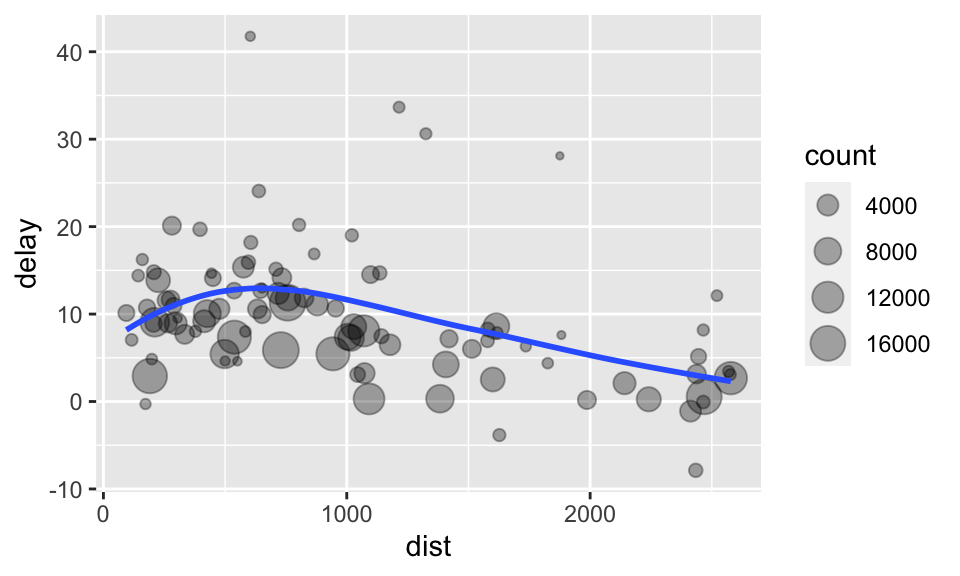
\includegraphics{R_learing_notes_files/figure-latex/unnamed-chunk-206-1} \end{center}

但這種撰寫程式碼的方式稍嫌惱人,因為我們還要幫中間的 data frame 取名字。使用 pipe \texttt{\%\textgreater{}\%} 可以解決此問題:

\begin{Shaded}
\begin{Highlighting}[]
\NormalTok{delays }\OtherTok{\textless{}{-}}\NormalTok{ flights }\SpecialCharTok{\%\textgreater{}\%}
  \FunctionTok{group\_by}\NormalTok{(dest) }\SpecialCharTok{\%\textgreater{}\%}
  \FunctionTok{summarize}\NormalTok{(}\AttributeTok{count =} \FunctionTok{n}\NormalTok{(),}
            \AttributeTok{dist =} \FunctionTok{mean}\NormalTok{(distance, }\AttributeTok{na.rm =} \ConstantTok{TRUE}\NormalTok{),}
            \AttributeTok{delay =} \FunctionTok{mean}\NormalTok{(arr\_delay, }\AttributeTok{na.rm =} \ConstantTok{TRUE}\NormalTok{)) }\SpecialCharTok{\%\textgreater{}\%}
  \FunctionTok{filter}\NormalTok{(count }\SpecialCharTok{\textgreater{}} \DecValTok{20}\NormalTok{, dest }\SpecialCharTok{!=} \StringTok{"HNL"}\NormalTok{)}
\end{Highlighting}
\end{Shaded}

\texttt{\%\textgreater{}\%} 可以讀成 ``then'',即我們先使用 \texttt{group\_by} 分組,然後使用 \texttt{summarize()} 計算次數與平均數,然後使用 \texttt{filter()} 過濾掉噪點與不想要的觀察值。這背後的邏輯就是 \texttt{x\ \%\textgreater{}\%\ f(y)} 即 \texttt{f(x,\ y)},而 \texttt{x\ \%\textgreater{}\%\ f(y)\ \%\textgreater{}\%\ g(z)} 即 \texttt{g(f(x,\ y),\ z)}。

\hypertarget{missingvaluesdplyr}{%
\subsection{缺漏值}\label{missingvaluesdplyr}}

前開使用的 \texttt{na.rm} 引數的功能即決定要不要在計算前移除掉 \texttt{NA}。如果我們沒有設定 \texttt{na.rm\ =\ TRUE},則我們將會製造出一大堆 \texttt{NA},因為 \texttt{NA} 無論做什麼運算都會得到 \texttt{NA},所以只要有其中一個觀察值的 \texttt{dep\_delay} 為 \texttt{NA},那一整天的平均就會是 \texttt{NA},如:

\begin{Shaded}
\begin{Highlighting}[]
\NormalTok{flights }\SpecialCharTok{\%\textgreater{}\%}
  \FunctionTok{group\_by}\NormalTok{(year, month, day) }\SpecialCharTok{\%\textgreater{}\%}
  \FunctionTok{summarize}\NormalTok{(}\AttributeTok{mean =} \FunctionTok{mean}\NormalTok{(dep\_delay)) }\SpecialCharTok{\%\textgreater{}\%}
  \FunctionTok{group\_by}\NormalTok{(mean) }\SpecialCharTok{\%\textgreater{}\%}
  \FunctionTok{summarize}\NormalTok{(}\AttributeTok{count =} \FunctionTok{n}\NormalTok{())}
\end{Highlighting}
\end{Shaded}

\begin{verbatim}
## `summarise()` has grouped output by 'year', 'month'. You can override using the `.groups` argument.
\end{verbatim}

\begin{verbatim}
## # A tibble: 8 x 2
##     mean count
##    <dbl> <int>
## 1  0.145     1
## 2  0.241     1
## 3  1.61      1
## 4  3.53      1
## 5  6.06      1
## 6  7.78      1
## 7  7.93      1
## 8 NA       358
\end{verbatim}

我們可以發現製造了 358 個 NA!以下就不會產生上面的問題了:

\begin{Shaded}
\begin{Highlighting}[]
\NormalTok{flights }\SpecialCharTok{\%\textgreater{}\%}
  \FunctionTok{group\_by}\NormalTok{(year, month, day) }\SpecialCharTok{\%\textgreater{}\%}
  \FunctionTok{summarize}\NormalTok{(}\AttributeTok{mean =} \FunctionTok{mean}\NormalTok{(dep\_delay, }\AttributeTok{na.rm =} \ConstantTok{TRUE}\NormalTok{))}
\end{Highlighting}
\end{Shaded}

在此,\texttt{NA} 代表航班取消;我們也可以先把 \texttt{NA} 的地方去除掉,如:

\begin{Shaded}
\begin{Highlighting}[]
\NormalTok{not\_cancelled }\OtherTok{\textless{}{-}}\NormalTok{ flights }\SpecialCharTok{\%\textgreater{}\%}
  \FunctionTok{filter}\NormalTok{(}\SpecialCharTok{!}\FunctionTok{is.na}\NormalTok{(dep\_delay), }\SpecialCharTok{!}\FunctionTok{is.na}\NormalTok{(arr\_delay))}

\NormalTok{not\_cancelled }\SpecialCharTok{\%\textgreater{}\%}
  \FunctionTok{group\_by}\NormalTok{(year, month, day) }\SpecialCharTok{\%\textgreater{}\%}
  \FunctionTok{summarize}\NormalTok{(}\AttributeTok{mean =} \FunctionTok{mean}\NormalTok{(dep\_delay))}
\end{Highlighting}
\end{Shaded}

\begin{verbatim}
## `summarise()` has grouped output by 'year', 'month'. You can override using the `.groups` argument.
\end{verbatim}

\begin{verbatim}
## # A tibble: 365 x 4
## # Groups:   year, month [12]
##     year month   day  mean
##    <int> <int> <int> <dbl>
##  1  2013     1     1 11.4 
##  2  2013     1     2 13.7 
##  3  2013     1     3 10.9 
##  4  2013     1     4  8.97
##  5  2013     1     5  5.73
##  6  2013     1     6  7.15
##  7  2013     1     7  5.42
##  8  2013     1     8  2.56
##  9  2013     1     9  2.30
## 10  2013     1    10  2.84
## # ... with 355 more rows
\end{verbatim}

\hypertarget{ux8a08ux6578}{%
\subsection{計數}\label{ux8a08ux6578}}

我們可以加入計數(\texttt{n()})或非缺漏值的計數(\texttt{sum(!is.na(x))}),避免我們從很小的樣本得出結論。

\begin{Shaded}
\begin{Highlighting}[]
\NormalTok{delays }\OtherTok{\textless{}{-}}\NormalTok{ not\_cancelled }\SpecialCharTok{\%\textgreater{}\%}
  \FunctionTok{group\_by}\NormalTok{(tailnum) }\SpecialCharTok{\%\textgreater{}\%}
  \FunctionTok{summarize}\NormalTok{(}\AttributeTok{delay =} \FunctionTok{mean}\NormalTok{(arr\_delay))}

\FunctionTok{ggplot}\NormalTok{(}\AttributeTok{data =}\NormalTok{ delays, }\AttributeTok{mapping =} \FunctionTok{aes}\NormalTok{(}\AttributeTok{x =}\NormalTok{ delay)) }\SpecialCharTok{+}
  \FunctionTok{geom\_freqpoly}\NormalTok{(}\AttributeTok{binwidth =} \DecValTok{10}\NormalTok{)}
\end{Highlighting}
\end{Shaded}

\begin{center}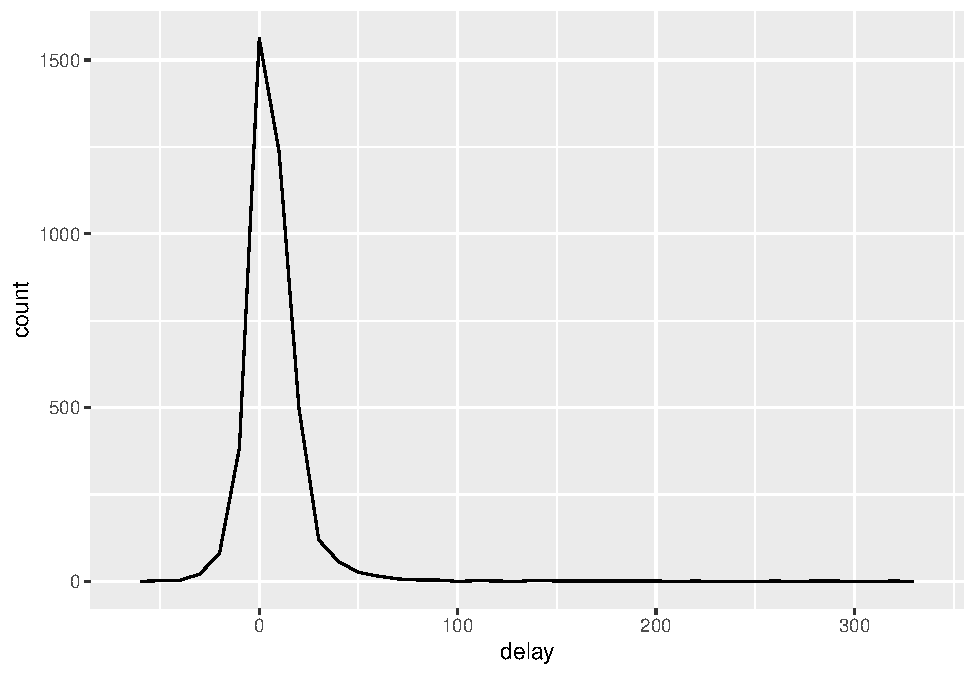
\includegraphics{R_learing_notes_files/figure-latex/unnamed-chunk-211-1} \end{center}

我們可以發現,有些航班甚至可以延遲超過 300 秒!但我們如果畫出散佈圖就會發現,如果只有少數幾個航班的日子,取平均以後其變異就會非常大,即樣本越大,變異越小(類似大數法則中,當樣本越來越大,估計參數會機率收斂到母體參數的概念),如:

\begin{Shaded}
\begin{Highlighting}[]
\NormalTok{delays }\OtherTok{\textless{}{-}}\NormalTok{ not\_cancelled }\SpecialCharTok{\%\textgreater{}\%}
  \FunctionTok{group\_by}\NormalTok{(tailnum) }\SpecialCharTok{\%\textgreater{}\%}
  \FunctionTok{summarize}\NormalTok{(}\AttributeTok{delay =} \FunctionTok{mean}\NormalTok{(arr\_delay, }\AttributeTok{na.rm =} \ConstantTok{TRUE}\NormalTok{),}\AttributeTok{n=}\FunctionTok{n}\NormalTok{())}

\FunctionTok{ggplot}\NormalTok{(}\AttributeTok{data =}\NormalTok{ delays, }\AttributeTok{mapping =} \FunctionTok{aes}\NormalTok{(}\AttributeTok{x =}\NormalTok{ n, }\AttributeTok{y =}\NormalTok{ delay)) }\SpecialCharTok{+}
  \FunctionTok{geom\_point}\NormalTok{(}\AttributeTok{alpha =} \DecValTok{1}\SpecialCharTok{/}\DecValTok{10}\NormalTok{)}
\end{Highlighting}
\end{Shaded}

\begin{center}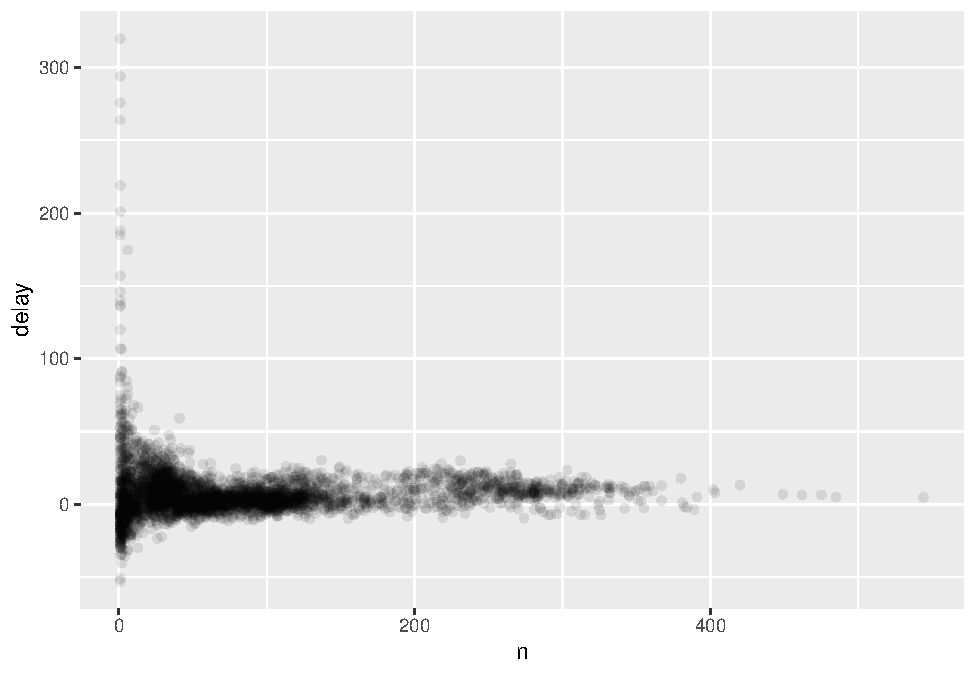
\includegraphics{R_learing_notes_files/figure-latex/unnamed-chunk-212-1} \end{center}

所以我們其實可以移除掉樣本過小的日期,如:

\begin{Shaded}
\begin{Highlighting}[]
\NormalTok{delays }\SpecialCharTok{\%\textgreater{}\%}
  \FunctionTok{filter}\NormalTok{(n }\SpecialCharTok{\textgreater{}} \DecValTok{25}\NormalTok{) }\SpecialCharTok{\%\textgreater{}\%}
  \FunctionTok{ggplot}\NormalTok{(}\AttributeTok{mapping =} \FunctionTok{aes}\NormalTok{(}\AttributeTok{x =}\NormalTok{ n, }\AttributeTok{y =}\NormalTok{ delay)) }\SpecialCharTok{+} \FunctionTok{geom\_point}\NormalTok{(}\AttributeTok{alpha =} \DecValTok{1}\SpecialCharTok{/}\DecValTok{10}\NormalTok{)}
\end{Highlighting}
\end{Shaded}

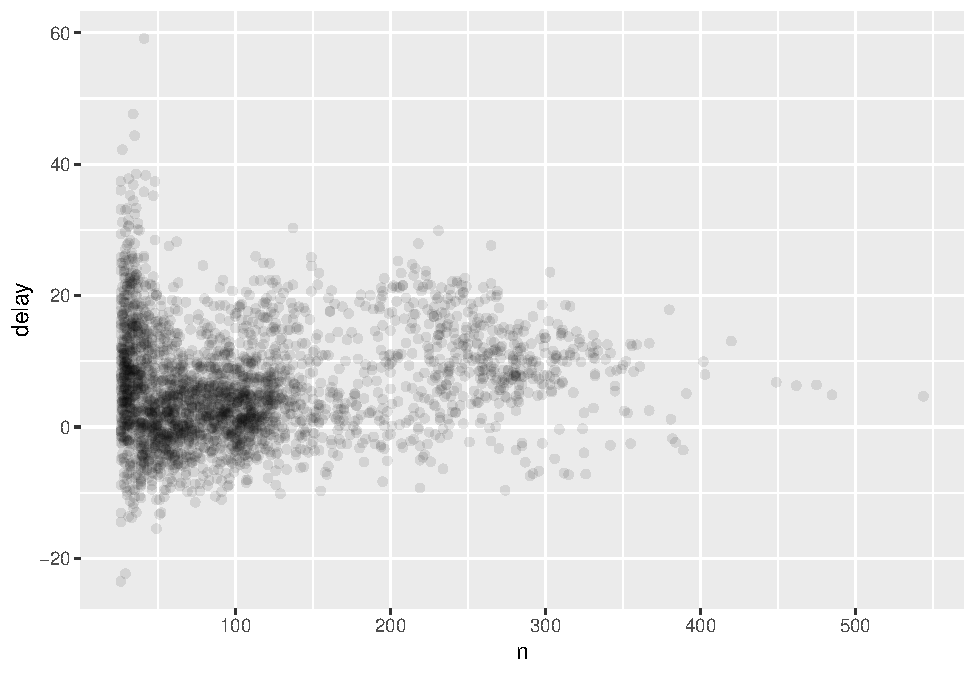
\includegraphics{R_learing_notes_files/figure-latex/unnamed-chunk-213-1.pdf}

我們接下來使用 \texttt{Lahman} 這個套件中的 \texttt{Batting} 這個 data frame 來討論棒球比賽中打擊者的表現與擊球次數的關係。

\begin{Shaded}
\begin{Highlighting}[]
\FunctionTok{library}\NormalTok{(Lahman)  }\CommentTok{\# 載入 Lahman}
\NormalTok{batting }\OtherTok{\textless{}{-}} \FunctionTok{as\_tibble}\NormalTok{(Lahman}\SpecialCharTok{::}\NormalTok{Batting)  }\CommentTok{\# 將 Batting 轉換成 tibble 型態}

\NormalTok{batters }\OtherTok{\textless{}{-}}\NormalTok{ batting }\SpecialCharTok{\%\textgreater{}\%}
  \FunctionTok{group\_by}\NormalTok{(playerID) }\SpecialCharTok{\%\textgreater{}\%}
  \FunctionTok{summarize}\NormalTok{(}\AttributeTok{ba =} \FunctionTok{sum}\NormalTok{(H, }\AttributeTok{na.rm =} \ConstantTok{TRUE}\NormalTok{) }\SpecialCharTok{/} \FunctionTok{sum}\NormalTok{(AB, }\AttributeTok{na.rm =} \ConstantTok{TRUE}\NormalTok{),}
            \AttributeTok{ab =} \FunctionTok{sum}\NormalTok{(AB, }\AttributeTok{na.rm =} \ConstantTok{TRUE}\NormalTok{) )}

\CommentTok{\# ba 為 batting average,即打擊率,衡量打擊的能力}
\CommentTok{\# ab 為 at bat,即上場打擊的機會}

\NormalTok{batters }\SpecialCharTok{\%\textgreater{}\%}
  \FunctionTok{filter}\NormalTok{(ab }\SpecialCharTok{\textgreater{}} \DecValTok{100}\NormalTok{) }\SpecialCharTok{\%\textgreater{}\%}
  \FunctionTok{ggplot}\NormalTok{(}\AttributeTok{mapping =} \FunctionTok{aes}\NormalTok{(}\AttributeTok{x =}\NormalTok{ ab, }\AttributeTok{y =}\NormalTok{ ba)) }\SpecialCharTok{+} \FunctionTok{geom\_point}\NormalTok{() }\SpecialCharTok{+}
    \FunctionTok{geom\_smooth}\NormalTok{(}\AttributeTok{se =} \ConstantTok{FALSE}\NormalTok{)}
\end{Highlighting}
\end{Shaded}

\begin{verbatim}
## `geom_smooth()` using method = 'gam' and formula 'y ~ s(x, bs = "cs")'
\end{verbatim}

\begin{center}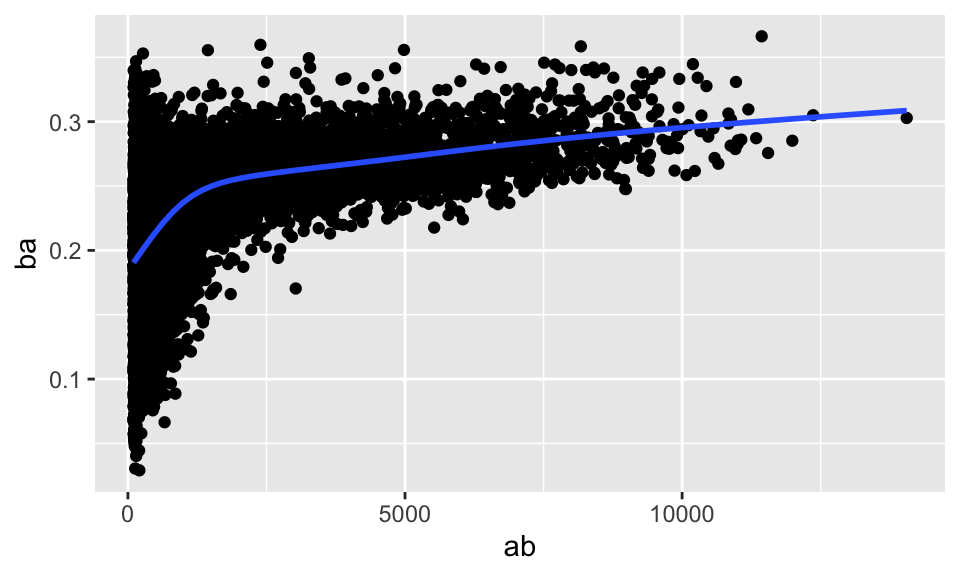
\includegraphics{R_learing_notes_files/figure-latex/unnamed-chunk-214-1} \end{center}

我們可以發現,打擊次數越多的球員,打擊率也就越高,兩者有正向的關係;這可能是因為球隊會讓能打球的球員上場。

\hypertarget{ux6709ux7528ux7684ux6b78ux7d0dux51fdux6578}{%
\subsection{有用的歸納函數}\label{ux6709ux7528ux7684ux6b78ux7d0dux51fdux6578}}

\begin{itemize}
\tightlist
\item
  \textbf{Measures of location:} \texttt{mean(x)}, \texttt{median(x)}.
\end{itemize}

\begin{Shaded}
\begin{Highlighting}[]
\NormalTok{not\_cancelled }\SpecialCharTok{\%\textgreater{}\%}
  \FunctionTok{group\_by}\NormalTok{(year, month, day) }\SpecialCharTok{\%\textgreater{}\%}
  \FunctionTok{summarize}\NormalTok{(}
    \CommentTok{\# average delay:}
    \AttributeTok{avg\_delay1 =} \FunctionTok{mean}\NormalTok{(arr\_delay),}
    \CommentTok{\# average positive delay:}
    \AttributeTok{avg\_delay2 =} \FunctionTok{mean}\NormalTok{(arr\_delay[arr\_delay }\SpecialCharTok{\textgreater{}} \DecValTok{0}\NormalTok{])}
\NormalTok{)}
\end{Highlighting}
\end{Shaded}

\begin{verbatim}
## `summarise()` has grouped output by 'year', 'month'. You can override using the `.groups` argument.
\end{verbatim}

\begin{verbatim}
## # A tibble: 365 x 5
## # Groups:   year, month [12]
##     year month   day avg_delay1 avg_delay2
##    <int> <int> <int>      <dbl>      <dbl>
##  1  2013     1     1     12.7         32.5
##  2  2013     1     2     12.7         32.0
##  3  2013     1     3      5.73        27.7
##  4  2013     1     4     -1.93        28.3
##  5  2013     1     5     -1.53        22.6
##  6  2013     1     6      4.24        24.4
##  7  2013     1     7     -4.95        27.8
##  8  2013     1     8     -3.23        20.8
##  9  2013     1     9     -0.264       25.6
## 10  2013     1    10     -5.90        27.3
## # ... with 355 more rows
\end{verbatim}

\begin{itemize}
\item
  \textbf{Measures of spread:} \texttt{sd(x)}, \texttt{IQR(x)}, \texttt{mad(x)}.

  \begin{itemize}
  \tightlist
  \item
    標準差、四分位距(interquartile range)與絕對中位差(median absolute deviation,即原數據減去中位數所得的新數據的絕對值的中位數)。
  \item
    \(\mbox{MAD} = \mbox{median}(|X_i - \mbox{median}|)\).
  \end{itemize}
\end{itemize}

\begin{Shaded}
\begin{Highlighting}[]
\CommentTok{\# 算出不同目的地的距離標準差,並降冪排列}
\NormalTok{not\_cancelled }\SpecialCharTok{\%\textgreater{}\%}
  \FunctionTok{group\_by}\NormalTok{(dest) }\SpecialCharTok{\%\textgreater{}\%}
  \FunctionTok{summarize}\NormalTok{(}\AttributeTok{distance\_sd =} \FunctionTok{sd}\NormalTok{(distance)) }\SpecialCharTok{\%\textgreater{}\%}
  \FunctionTok{arrange}\NormalTok{(}\FunctionTok{desc}\NormalTok{(distance\_sd))}
\end{Highlighting}
\end{Shaded}

\begin{verbatim}
## # A tibble: 104 x 2
##    dest  distance_sd
##    <chr>       <dbl>
##  1 EGE         10.5 
##  2 SAN         10.4 
##  3 SFO         10.2 
##  4 HNL         10.0 
##  5 SEA          9.98
##  6 LAS          9.91
##  7 PDX          9.87
##  8 PHX          9.86
##  9 LAX          9.66
## 10 IND          9.46
## # ... with 94 more rows
\end{verbatim}

\begin{itemize}
\item
  \textbf{Measures of rank:} \texttt{min(x)}, \texttt{quantile(x,\ 0.25)}, \texttt{max(x)}.

  \begin{itemize}
  \tightlist
  \item
    \texttt{quantile(x,\ 0.25)} 即大於 25 \% 的樣本但小於剩餘的 75 \% 者。
  \end{itemize}
\end{itemize}

\begin{Shaded}
\begin{Highlighting}[]
\CommentTok{\# 算出每天第一班與最後一班班機}
\NormalTok{not\_cancelled }\SpecialCharTok{\%\textgreater{}\%}
  \FunctionTok{group\_by}\NormalTok{(year, month, day) }\SpecialCharTok{\%\textgreater{}\%}
  \FunctionTok{summarize}\NormalTok{(}
    \AttributeTok{first =} \FunctionTok{min}\NormalTok{(dep\_time),}
    \AttributeTok{last =} \FunctionTok{max}\NormalTok{(dep\_time)}
\NormalTok{  )}
\end{Highlighting}
\end{Shaded}

\begin{verbatim}
## `summarise()` has grouped output by 'year', 'month'. You can override using the `.groups` argument.
\end{verbatim}

\begin{verbatim}
## # A tibble: 365 x 5
## # Groups:   year, month [12]
##     year month   day first  last
##    <int> <int> <int> <int> <int>
##  1  2013     1     1   517  2356
##  2  2013     1     2    42  2354
##  3  2013     1     3    32  2349
##  4  2013     1     4    25  2358
##  5  2013     1     5    14  2357
##  6  2013     1     6    16  2355
##  7  2013     1     7    49  2359
##  8  2013     1     8   454  2351
##  9  2013     1     9     2  2252
## 10  2013     1    10     3  2320
## # ... with 355 more rows
\end{verbatim}

\begin{itemize}
\tightlist
\item
  \textbf{Measures of position:} \texttt{first(x)}, \texttt{nth(x,\ 2)}, \texttt{last(x)}.
\end{itemize}

\begin{Shaded}
\begin{Highlighting}[]
\CommentTok{\# 找出每天第一班與最後一班班機}
\NormalTok{not\_cancelled }\SpecialCharTok{\%\textgreater{}\%}
  \FunctionTok{group\_by}\NormalTok{(year, month, day) }\SpecialCharTok{\%\textgreater{}\%}
  \FunctionTok{summarize}\NormalTok{(}
    \AttributeTok{first =} \FunctionTok{min}\NormalTok{(dep\_time),}
    \AttributeTok{last =} \FunctionTok{max}\NormalTok{(dep\_time)}
\NormalTok{  )}
\end{Highlighting}
\end{Shaded}

\begin{verbatim}
## `summarise()` has grouped output by 'year', 'month'. You can override using the `.groups` argument.
\end{verbatim}

\begin{verbatim}
## # A tibble: 365 x 5
## # Groups:   year, month [12]
##     year month   day first  last
##    <int> <int> <int> <int> <int>
##  1  2013     1     1   517  2356
##  2  2013     1     2    42  2354
##  3  2013     1     3    32  2349
##  4  2013     1     4    25  2358
##  5  2013     1     5    14  2357
##  6  2013     1     6    16  2355
##  7  2013     1     7    49  2359
##  8  2013     1     8   454  2351
##  9  2013     1     9     2  2252
## 10  2013     1    10     3  2320
## # ... with 355 more rows
\end{verbatim}

\begin{Shaded}
\begin{Highlighting}[]
\NormalTok{not\_cancelled }\SpecialCharTok{\%\textgreater{}\%}
  \FunctionTok{group\_by}\NormalTok{(year, month, day) }\SpecialCharTok{\%\textgreater{}\%}
  \FunctionTok{mutate}\NormalTok{(}\AttributeTok{r =} \FunctionTok{min\_rank}\NormalTok{(}\FunctionTok{desc}\NormalTok{(dep\_time))) }\SpecialCharTok{\%\textgreater{}\%}
  \FunctionTok{filter}\NormalTok{(r }\SpecialCharTok{\%in\%} \FunctionTok{range}\NormalTok{(r))}
\end{Highlighting}
\end{Shaded}

\begin{verbatim}
## # A tibble: 770 x 20
## # Groups:   year, month, day [365]
##     year month   day dep_time sched_dep_time dep_delay arr_time sched_arr_time
##    <int> <int> <int>    <int>          <int>     <dbl>    <int>          <int>
##  1  2013     1     1      517            515         2      830            819
##  2  2013     1     1     2356           2359        -3      425            437
##  3  2013     1     2       42           2359        43      518            442
##  4  2013     1     2     2354           2359        -5      413            437
##  5  2013     1     3       32           2359        33      504            442
##  6  2013     1     3     2349           2359       -10      434            445
##  7  2013     1     4       25           2359        26      505            442
##  8  2013     1     4     2358           2359        -1      429            437
##  9  2013     1     4     2358           2359        -1      436            445
## 10  2013     1     5       14           2359        15      503            445
## # ... with 760 more rows, and 12 more variables: arr_delay <dbl>,
## #   carrier <chr>, flight <int>, tailnum <chr>, origin <chr>, dest <chr>,
## #   air_time <dbl>, distance <dbl>, hour <dbl>, minute <dbl>, time_hour <dttm>,
## #   r <int>
\end{verbatim}

\begin{itemize}
\item
  \textbf{Counts:} \texttt{n()}, \texttt{sum(!is.na(x))}, \texttt{n\_distinct(x):}.

  \begin{itemize}
  \tightlist
  \item
    \texttt{sum(!is.na(x))}: non-missing values.
  \item
    \texttt{n\_distinct(x)}: the number of distinct (unique) values.
  \end{itemize}
\end{itemize}

\begin{Shaded}
\begin{Highlighting}[]
\NormalTok{not\_cancelled }\SpecialCharTok{\%\textgreater{}\%}
  \FunctionTok{group\_by}\NormalTok{(dest) }\SpecialCharTok{\%\textgreater{}\%}
  \FunctionTok{summarize}\NormalTok{(}\AttributeTok{carriers =} \FunctionTok{n\_distinct}\NormalTok{(carrier)) }\SpecialCharTok{\%\textgreater{}\%}
  \FunctionTok{arrange}\NormalTok{(}\FunctionTok{desc}\NormalTok{(carriers))}
\end{Highlighting}
\end{Shaded}

\begin{verbatim}
## # A tibble: 104 x 2
##    dest  carriers
##    <chr>    <int>
##  1 ATL          7
##  2 BOS          7
##  3 CLT          7
##  4 ORD          7
##  5 TPA          7
##  6 AUS          6
##  7 DCA          6
##  8 DTW          6
##  9 IAD          6
## 10 MSP          6
## # ... with 94 more rows
\end{verbatim}

\begin{Shaded}
\begin{Highlighting}[]
\CommentTok{\# 因為 count() 太常用了}
\CommentTok{\# 所以甚至不用 summerize() 就可以直接使用}
\NormalTok{not\_cancelled }\SpecialCharTok{\%\textgreater{}\%}
  \FunctionTok{count}\NormalTok{(dest)}
\end{Highlighting}
\end{Shaded}

\begin{Shaded}
\begin{Highlighting}[]
\CommentTok{\# 甚至可以在引數 wt 加上權重}
\CommentTok{\# 如下算出各飛機的總里程}
\NormalTok{not\_cancelled }\SpecialCharTok{\%\textgreater{}\%}
  \FunctionTok{count}\NormalTok{(tailnum, }\AttributeTok{wt =}\NormalTok{ distance)}
\end{Highlighting}
\end{Shaded}

\begin{verbatim}
## # A tibble: 4,037 x 2
##    tailnum      n
##    <chr>    <dbl>
##  1 D942DN    3418
##  2 N0EGMQ  239143
##  3 N10156  109664
##  4 N102UW   25722
##  5 N103US   24619
##  6 N104UW   24616
##  7 N10575  139903
##  8 N105UW   23618
##  9 N107US   21677
## 10 N108UW   32070
## # ... with 4,027 more rows
\end{verbatim}

\begin{itemize}
\item
  \textbf{Counts and proportions of logical values:} \texttt{sum(x\ \textgreater{}\ 10)}, \texttt{mean(y\ ==\ 0)}.

  \begin{itemize}
  \tightlist
  \item
    如果這些邏輯判斷式為真,那就會回傳 \texttt{TRUE},反之則回傳 \texttt{FALSE}。
  \item
    據此,我們可以使用 \texttt{sum()} 來得知符合這些條件的有多少,而使用 \texttt{mean()} 來得知符合條件的比例。
  \end{itemize}
\end{itemize}

\begin{Shaded}
\begin{Highlighting}[]
\CommentTok{\# 如果我們想得知每天離開時間小於 500 的班次數目,可以如下}
\NormalTok{not\_cancelled }\SpecialCharTok{\%\textgreater{}\%}
  \FunctionTok{group\_by}\NormalTok{(year, month, day) }\SpecialCharTok{\%\textgreater{}\%}
  \FunctionTok{summarize}\NormalTok{(}\AttributeTok{n\_early =} \FunctionTok{sum}\NormalTok{(dep\_time }\SpecialCharTok{\textless{}} \DecValTok{500}\NormalTok{))}
\end{Highlighting}
\end{Shaded}

\begin{verbatim}
## `summarise()` has grouped output by 'year', 'month'. You can override using the `.groups` argument.
\end{verbatim}

\begin{verbatim}
## # A tibble: 365 x 4
## # Groups:   year, month [12]
##     year month   day n_early
##    <int> <int> <int>   <int>
##  1  2013     1     1       0
##  2  2013     1     2       3
##  3  2013     1     3       4
##  4  2013     1     4       3
##  5  2013     1     5       3
##  6  2013     1     6       2
##  7  2013     1     7       2
##  8  2013     1     8       1
##  9  2013     1     9       3
## 10  2013     1    10       3
## # ... with 355 more rows
\end{verbatim}

\begin{Shaded}
\begin{Highlighting}[]
\CommentTok{\# 如果我們想得知每天延誤超過一小時的航班的比例,可以如下}
\NormalTok{not\_cancelled }\SpecialCharTok{\%\textgreater{}\%}
  \FunctionTok{group\_by}\NormalTok{(year, month, day) }\SpecialCharTok{\%\textgreater{}\%}
  \FunctionTok{summarize}\NormalTok{(}\AttributeTok{hour\_perc =} \FunctionTok{mean}\NormalTok{(arr\_delay }\SpecialCharTok{\textgreater{}} \DecValTok{60}\NormalTok{))}
\end{Highlighting}
\end{Shaded}

\begin{verbatim}
## `summarise()` has grouped output by 'year', 'month'. You can override using the `.groups` argument.
\end{verbatim}

\begin{verbatim}
## # A tibble: 365 x 4
## # Groups:   year, month [12]
##     year month   day hour_perc
##    <int> <int> <int>     <dbl>
##  1  2013     1     1    0.0722
##  2  2013     1     2    0.0851
##  3  2013     1     3    0.0567
##  4  2013     1     4    0.0396
##  5  2013     1     5    0.0349
##  6  2013     1     6    0.0470
##  7  2013     1     7    0.0333
##  8  2013     1     8    0.0213
##  9  2013     1     9    0.0202
## 10  2013     1    10    0.0183
## # ... with 355 more rows
\end{verbatim}

\hypertarget{ux4f9dux64daux591aux8b8aux6578ux5206ux7d44}{%
\subsection{依據多變數分組}\label{ux4f9dux64daux591aux8b8aux6578ux5206ux7d44}}

像撥洋蔥一樣,但不太可能適用於有牽涉到排序的統計量,如中位數。

\begin{Shaded}
\begin{Highlighting}[]
\NormalTok{daily }\OtherTok{\textless{}{-}} \FunctionTok{group\_by}\NormalTok{(flights, year, month, day)}
\NormalTok{(per\_day }\OtherTok{\textless{}{-}}\FunctionTok{summarize}\NormalTok{(daily,}\AttributeTok{flights=}\FunctionTok{n}\NormalTok{()))}
\end{Highlighting}
\end{Shaded}

\begin{verbatim}
## `summarise()` has grouped output by 'year', 'month'. You can override using the `.groups` argument.
\end{verbatim}

\begin{verbatim}
## # A tibble: 365 x 4
## # Groups:   year, month [12]
##     year month   day flights
##    <int> <int> <int>   <int>
##  1  2013     1     1     842
##  2  2013     1     2     943
##  3  2013     1     3     914
##  4  2013     1     4     915
##  5  2013     1     5     720
##  6  2013     1     6     832
##  7  2013     1     7     933
##  8  2013     1     8     899
##  9  2013     1     9     902
## 10  2013     1    10     932
## # ... with 355 more rows
\end{verbatim}

\begin{Shaded}
\begin{Highlighting}[]
\NormalTok{(per\_month }\OtherTok{\textless{}{-}} \FunctionTok{summarize}\NormalTok{(per\_day, }\AttributeTok{flights =} \FunctionTok{sum}\NormalTok{(flights)))}
\end{Highlighting}
\end{Shaded}

\begin{verbatim}
## `summarise()` has grouped output by 'year'. You can override using the `.groups` argument.
\end{verbatim}

\begin{verbatim}
## # A tibble: 12 x 3
## # Groups:   year [1]
##     year month flights
##    <int> <int>   <int>
##  1  2013     1   27004
##  2  2013     2   24951
##  3  2013     3   28834
##  4  2013     4   28330
##  5  2013     5   28796
##  6  2013     6   28243
##  7  2013     7   29425
##  8  2013     8   29327
##  9  2013     9   27574
## 10  2013    10   28889
## 11  2013    11   27268
## 12  2013    12   28135
\end{verbatim}

\begin{Shaded}
\begin{Highlighting}[]
\NormalTok{(per\_year }\OtherTok{\textless{}{-}} \FunctionTok{summarize}\NormalTok{(per\_month, }\AttributeTok{flights =} \FunctionTok{sum}\NormalTok{(flights)))}
\end{Highlighting}
\end{Shaded}

\begin{verbatim}
## # A tibble: 1 x 2
##    year flights
##   <int>   <int>
## 1  2013  336776
\end{verbatim}

\hypertarget{ux53d6ux6d88ux5206ux7d44}{%
\subsection{取消分組}\label{ux53d6ux6d88ux5206ux7d44}}

使用 \texttt{ungroup()} 可以取消分組,如下:

\begin{Shaded}
\begin{Highlighting}[]
\NormalTok{daily }\SpecialCharTok{\%\textgreater{}\%}
  \FunctionTok{ungroup}\NormalTok{() }\SpecialCharTok{\%\textgreater{}\%} \CommentTok{\# no longer grouped by date}
  \FunctionTok{summarize}\NormalTok{(}\AttributeTok{flights =} \FunctionTok{n}\NormalTok{())}
\end{Highlighting}
\end{Shaded}

\begin{verbatim}
## # A tibble: 1 x 1
##   flights
##     <int>
## 1  336776
\end{verbatim}

\hypertarget{grouped-mutates-and-filters}{%
\section{Grouped Mutates (and Filters)}\label{grouped-mutates-and-filters}}

除了與 \texttt{summarize()} 共同使用,\texttt{group\_by} 與 \texttt{mutate()} 及 \texttt{filter()} 共同使用也很方便,例如:

\begin{itemize}
\tightlist
\item
  找每組最差的成員:
\end{itemize}

\begin{Shaded}
\begin{Highlighting}[]
\NormalTok{flights\_sml }\SpecialCharTok{\%\textgreater{}\%}
  \FunctionTok{group\_by}\NormalTok{(year, month, day) }\SpecialCharTok{\%\textgreater{}\%}
  \FunctionTok{filter}\NormalTok{(}\FunctionTok{rank}\NormalTok{(}\FunctionTok{desc}\NormalTok{(arr\_delay)) }\SpecialCharTok{\textless{}} \DecValTok{10}\NormalTok{)}
\end{Highlighting}
\end{Shaded}

\begin{verbatim}
## # A tibble: 3,306 x 7
## # Groups:   year, month, day [365]
##     year month   day dep_delay arr_delay distance air_time
##    <int> <int> <int>     <dbl>     <dbl>    <dbl>    <dbl>
##  1  2013     1     1       853       851      184       41
##  2  2013     1     1       290       338     1134      213
##  3  2013     1     1       260       263      266       46
##  4  2013     1     1       157       174      213       60
##  5  2013     1     1       216       222      708      121
##  6  2013     1     1       255       250      589      115
##  7  2013     1     1       285       246     1085      146
##  8  2013     1     1       192       191      199       44
##  9  2013     1     1       379       456     1092      222
## 10  2013     1     2       224       207      550       94
## # ... with 3,296 more rows
\end{verbatim}

\begin{itemize}
\tightlist
\item
  找到所有大於某個閾值的組別:
\end{itemize}

\begin{Shaded}
\begin{Highlighting}[]
\NormalTok{popular\_dests }\OtherTok{\textless{}{-}}\NormalTok{ flights }\SpecialCharTok{\%\textgreater{}\%}
  \FunctionTok{group\_by}\NormalTok{(dest) }\SpecialCharTok{\%\textgreater{}\%}
  \FunctionTok{filter}\NormalTok{(}\FunctionTok{n}\NormalTok{() }\SpecialCharTok{\textgreater{}} \DecValTok{365}\NormalTok{)}
\NormalTok{popular\_dests}
\end{Highlighting}
\end{Shaded}

\begin{verbatim}
## # A tibble: 332,577 x 19
## # Groups:   dest [77]
##     year month   day dep_time sched_dep_time dep_delay arr_time sched_arr_time
##    <int> <int> <int>    <int>          <int>     <dbl>    <int>          <int>
##  1  2013     1     1      517            515         2      830            819
##  2  2013     1     1      533            529         4      850            830
##  3  2013     1     1      542            540         2      923            850
##  4  2013     1     1      544            545        -1     1004           1022
##  5  2013     1     1      554            600        -6      812            837
##  6  2013     1     1      554            558        -4      740            728
##  7  2013     1     1      555            600        -5      913            854
##  8  2013     1     1      557            600        -3      709            723
##  9  2013     1     1      557            600        -3      838            846
## 10  2013     1     1      558            600        -2      753            745
## # ... with 332,567 more rows, and 11 more variables: arr_delay <dbl>,
## #   carrier <chr>, flight <int>, tailnum <chr>, origin <chr>, dest <chr>,
## #   air_time <dbl>, distance <dbl>, hour <dbl>, minute <dbl>, time_hour <dttm>
\end{verbatim}

\begin{itemize}
\tightlist
\item
  標準化:
\end{itemize}

\begin{Shaded}
\begin{Highlighting}[]
\NormalTok{popular\_dests }\SpecialCharTok{\%\textgreater{}\%}
  \FunctionTok{filter}\NormalTok{(arr\_delay }\SpecialCharTok{\textgreater{}} \DecValTok{0}\NormalTok{) }\SpecialCharTok{\%\textgreater{}\%}
  \FunctionTok{mutate}\NormalTok{(}\AttributeTok{prop\_delay =}\NormalTok{ arr\_delay }\SpecialCharTok{/} \FunctionTok{sum}\NormalTok{(arr\_delay)) }\SpecialCharTok{\%\textgreater{}\%}
  \FunctionTok{select}\NormalTok{(year}\SpecialCharTok{:}\NormalTok{day, dest, arr\_delay, prop\_delay)}
\end{Highlighting}
\end{Shaded}

\begin{verbatim}
## # A tibble: 131,106 x 6
## # Groups:   dest [77]
##     year month   day dest  arr_delay prop_delay
##    <int> <int> <int> <chr>     <dbl>      <dbl>
##  1  2013     1     1 IAH          11  0.000111 
##  2  2013     1     1 IAH          20  0.000201 
##  3  2013     1     1 MIA          33  0.000235 
##  4  2013     1     1 ORD          12  0.0000424
##  5  2013     1     1 FLL          19  0.0000938
##  6  2013     1     1 ORD           8  0.0000283
##  7  2013     1     1 LAX           7  0.0000344
##  8  2013     1     1 DFW          31  0.000282 
##  9  2013     1     1 ATL          12  0.0000400
## 10  2013     1     1 DTW          16  0.000116 
## # ... with 131,096 more rows
\end{verbatim}

\hypertarget{ux63a2ux7d22ux6027ux8cc7ux6599ux5206ux6790}{%
\chapter{探索性資料分析}\label{ux63a2ux7d22ux6027ux8cc7ux6599ux5206ux6790}}

\begin{quote}
資料一拿來就先跑跑看長什麼樣子!
\end{quote}

\hypertarget{ux4e8bux524dux6e96ux5099}{%
\section{事前準備}\label{ux4e8bux524dux6e96ux5099}}

探索性資料分析(Exploratory Data Analysis, EDA)的目標就是要更了解資料,而步驟可以為:

\begin{enumerate}
\def\labelenumi{\arabic{enumi}.}
\item
  構思關於這筆資料的問題。
\item
  透過視覺化、轉換和建模,試著尋找答案。
\item
  經由所得的結果,重整原先的問題,或者構思、增加新的問題。
\end{enumerate}

\hypertarget{ux554fux984c}{%
\section{問題}\label{ux554fux984c}}

\begin{quote}
Far better an approximate answer to the right question, which is often vague, than an exact answer to the wrong question, which can always be made precise.

---John Tukey
\end{quote}

你可以問這兩類的問題:

\begin{enumerate}
\def\labelenumi{\arabic{enumi}.}
\item
  What type of variation occurs within my variables?
\item
  What type of covariation occurs between my variables?
\end{enumerate}

\hypertarget{variation}{%
\section{Variation}\label{variation}}

Variation 即每次測量變數值所得的趨勢(tendency)。每個變數都有自己的 variation,而要看出 variation,最好的方法是視覺化變數值的分配。

\hypertarget{ux8996ux89baux5316ux5206ux914d}{%
\subsection{視覺化分配}\label{ux8996ux89baux5316ux5206ux914d}}

如果是\textbf{類別變數},我們可以使用 bar chart 來視覺化,因為它只有一小組變數值,而存成 factors 或 characters 的向量,如:

\begin{Shaded}
\begin{Highlighting}[]
\FunctionTok{ggplot}\NormalTok{(}\AttributeTok{data =}\NormalTok{ diamonds) }\SpecialCharTok{+}
  \FunctionTok{geom\_bar}\NormalTok{(}\AttributeTok{mapping =} \FunctionTok{aes}\NormalTok{(}\AttributeTok{x =}\NormalTok{ cut))}
\end{Highlighting}
\end{Shaded}

\begin{center}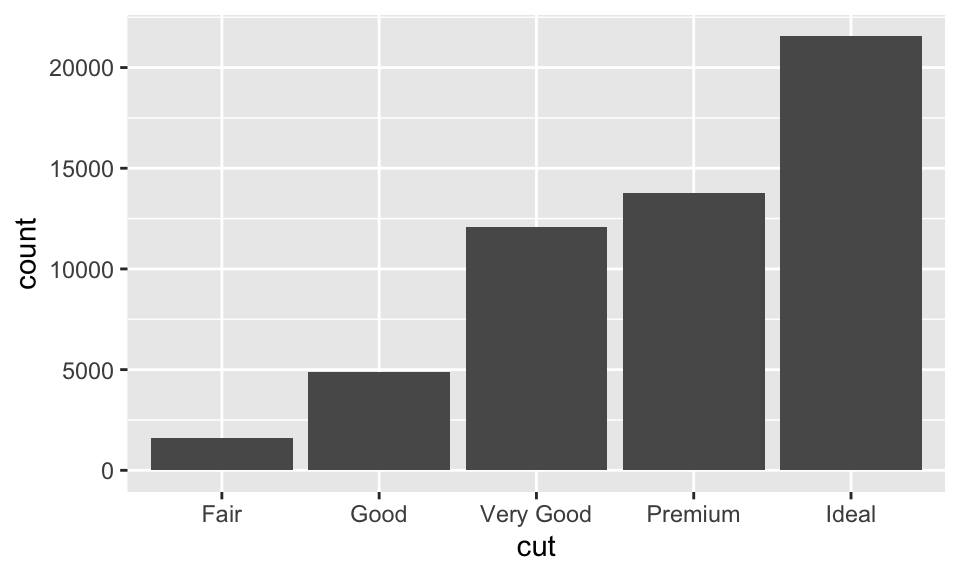
\includegraphics{R_learing_notes_files/figure-latex/unnamed-chunk-230-1} \end{center}

也可以使用 \texttt{dplyr} 的 \texttt{count()} 來計算究竟各種品質的鑽石有多少,如:

\begin{Shaded}
\begin{Highlighting}[]
\NormalTok{diamonds }\SpecialCharTok{\%\textgreater{}\%}
  \FunctionTok{count}\NormalTok{(cut)}
\end{Highlighting}
\end{Shaded}

\begin{verbatim}
## # A tibble: 5 x 2
##   cut           n
##   <ord>     <int>
## 1 Fair       1610
## 2 Good       4906
## 3 Very Good 12082
## 4 Premium   13791
## 5 Ideal     21551
\end{verbatim}

如果是\textbf{連續變數},例如數字與日期時間,我們則要使用 histogram,如:

\begin{Shaded}
\begin{Highlighting}[]
\CommentTok{\# binwidth 引數即直方圖的直方寬度}
\FunctionTok{ggplot}\NormalTok{(}\AttributeTok{data =}\NormalTok{ diamonds) }\SpecialCharTok{+}
  \FunctionTok{geom\_histogram}\NormalTok{(}\AttributeTok{mapping =} \FunctionTok{aes}\NormalTok{(}\AttributeTok{x =}\NormalTok{ carat), }\AttributeTok{binwidth =} \FloatTok{0.5}\NormalTok{)}
\end{Highlighting}
\end{Shaded}

\begin{center}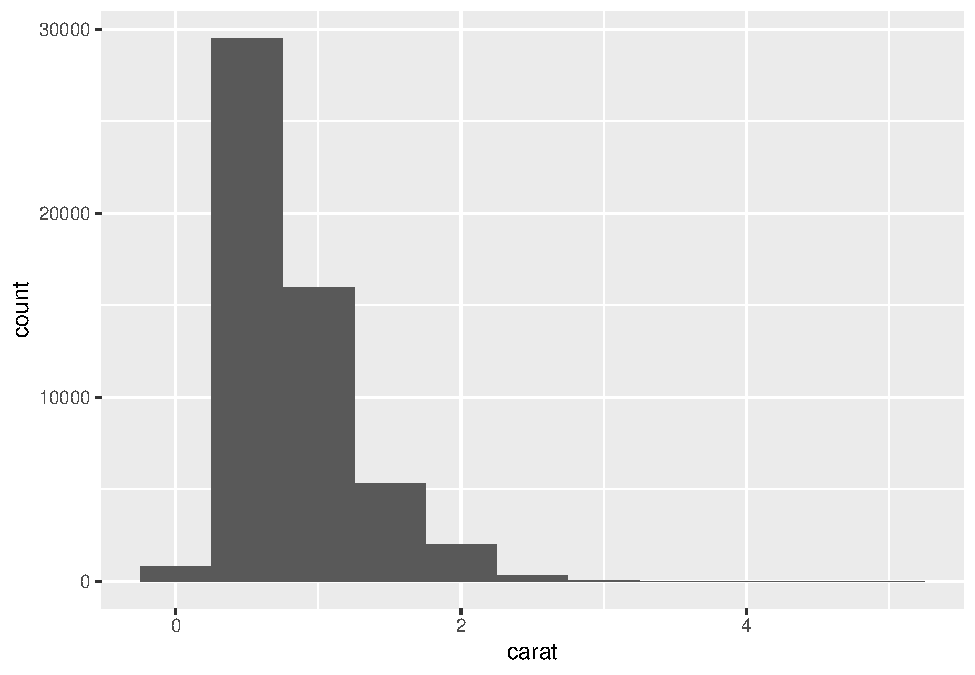
\includegraphics{R_learing_notes_files/figure-latex/unnamed-chunk-232-1} \end{center}

我們也可以用 \texttt{count()} 來計算,如:

\begin{Shaded}
\begin{Highlighting}[]
\NormalTok{diamonds }\SpecialCharTok{\%\textgreater{}\%}
  \FunctionTok{count}\NormalTok{(}\FunctionTok{cut\_width}\NormalTok{(carat, }\FloatTok{0.5}\NormalTok{))}
\end{Highlighting}
\end{Shaded}

\begin{verbatim}
## # A tibble: 11 x 2
##    `cut_width(carat, 0.5)`     n
##    <fct>                   <int>
##  1 [-0.25,0.25]              785
##  2 (0.25,0.75]             29498
##  3 (0.75,1.25]             15977
##  4 (1.25,1.75]              5313
##  5 (1.75,2.25]              2002
##  6 (2.25,2.75]               322
##  7 (2.75,3.25]                32
##  8 (3.25,3.75]                 5
##  9 (3.75,4.25]                 4
## 10 (4.25,4.75]                 1
## 11 (4.75,5.25]                 1
\end{verbatim}

如果想要重疊多個直方圖,使用 \texttt{geom\_frepoly()} 而非 \texttt{geom\_histogram()}。兩者的算法一樣,但前者以線來呈現,後者以直方來呈現,如:

\begin{Shaded}
\begin{Highlighting}[]
\FunctionTok{ggplot}\NormalTok{(}\AttributeTok{data =}\NormalTok{ diamonds, }\AttributeTok{mapping =} \FunctionTok{aes}\NormalTok{(}\AttributeTok{x =}\NormalTok{ carat, }\AttributeTok{color =}\NormalTok{ cut)) }\SpecialCharTok{+}
  \FunctionTok{geom\_freqpoly}\NormalTok{(}\AttributeTok{binwidth =} \FloatTok{0.1}\NormalTok{)}
\end{Highlighting}
\end{Shaded}

\begin{center}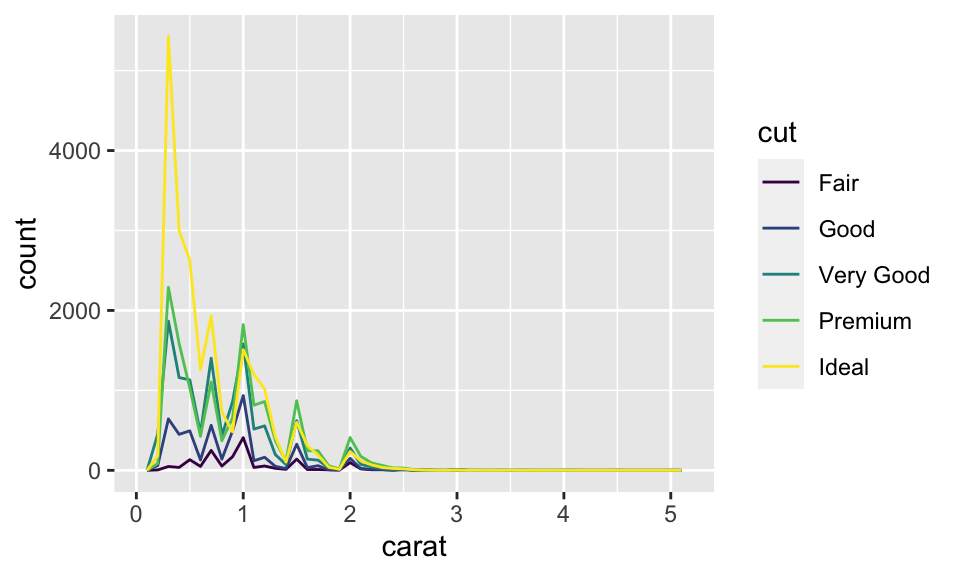
\includegraphics{R_learing_notes_files/figure-latex/unnamed-chunk-234-1} \end{center}

\hypertarget{ux4ee3ux8868ux6027ux7684ux8b8aux6578ux503c}{%
\subsection{代表性的變數值}\label{ux4ee3ux8868ux6027ux7684ux8b8aux6578ux503c}}

哪些是變數值經常出現?哪些變數值很少出現?其中有什麼規律?

\begin{Shaded}
\begin{Highlighting}[]
\FunctionTok{ggplot}\NormalTok{(}\AttributeTok{data =}\NormalTok{ diamonds, }\AttributeTok{mapping =} \FunctionTok{aes}\NormalTok{(}\AttributeTok{x =}\NormalTok{ carat)) }\SpecialCharTok{+}
  \FunctionTok{geom\_histogram}\NormalTok{(}\AttributeTok{binwidth =} \FloatTok{0.01}\NormalTok{)}
\end{Highlighting}
\end{Shaded}

\begin{center}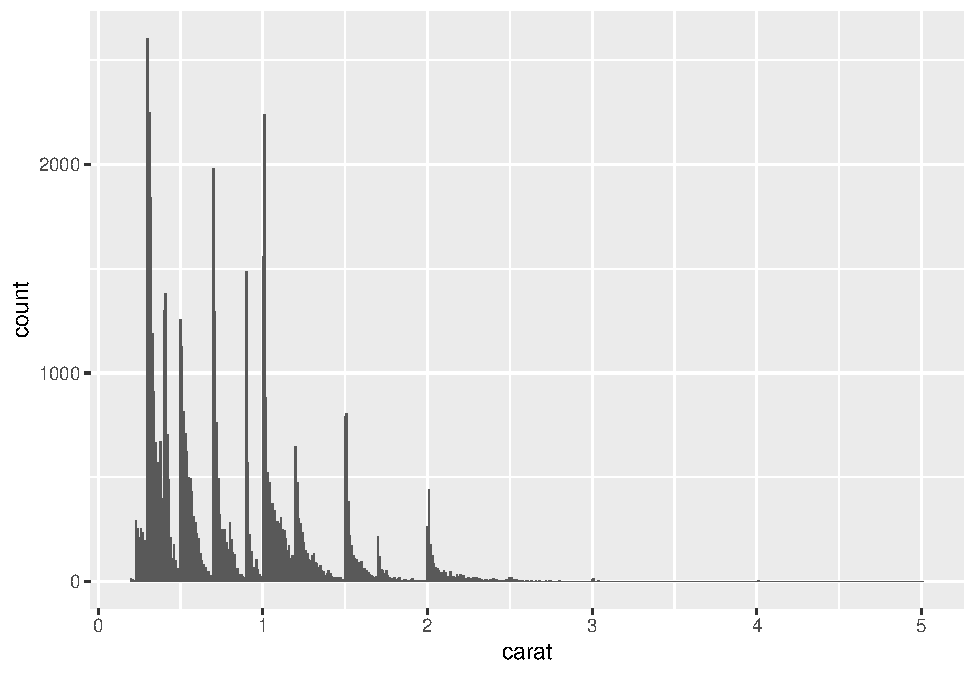
\includegraphics{R_learing_notes_files/figure-latex/unnamed-chunk-235-1} \end{center}

為何克拉數為整數與某些常見的有理數的觀察值特別多?為何每個高峰的右側都比左側更緩?為何超過 3 克拉的鑽石很稀有?

類似的值的群集(cluster)通常意味著資料中有子群(subgroup)。我們可以質問幾個問題:

\begin{enumerate}
\def\labelenumi{\arabic{enumi}.}
\item
  每個 subgroup 中的觀察值與其他 subgroups 之間有何相異或相似?
\item
  如何描述或解釋群集?
\item
  為何群集的外觀可能產生誤導?
\end{enumerate}

\hypertarget{ux4e0dux5c0bux5e38ux7684ux8b8aux6578ux503c}{%
\subsection{不尋常的變數值}\label{ux4e0dux5c0bux5e38ux7684ux8b8aux6578ux503c}}

Outliers 即不尋常的變數值,可能源自資料輸入錯誤,也可能是一些不一樣的東西。

要注意的是,當樣本很大時,使用直方圖很難看出 outliers;例如上一張圖中,事實上 3 克拉到 5 克拉之間都還有觀察值,可是從直方圖幾乎看不出來。我們可以透過 \texttt{coord\_cartesian()},來改變 y 軸的上下限,這樣就可以辨識稀有的觀察值了,如:

\begin{Shaded}
\begin{Highlighting}[]
\FunctionTok{ggplot}\NormalTok{(diamonds) }\SpecialCharTok{+}
  \FunctionTok{geom\_histogram}\NormalTok{(}\AttributeTok{mapping =} \FunctionTok{aes}\NormalTok{(}\AttributeTok{x =}\NormalTok{ y), }\AttributeTok{binwidth =} \FloatTok{0.5}\NormalTok{) }\SpecialCharTok{+}
  \FunctionTok{coord\_cartesian}\NormalTok{(}\AttributeTok{ylim =} \FunctionTok{c}\NormalTok{(}\DecValTok{0}\NormalTok{, }\DecValTok{50}\NormalTok{))}
\end{Highlighting}
\end{Shaded}

\begin{center}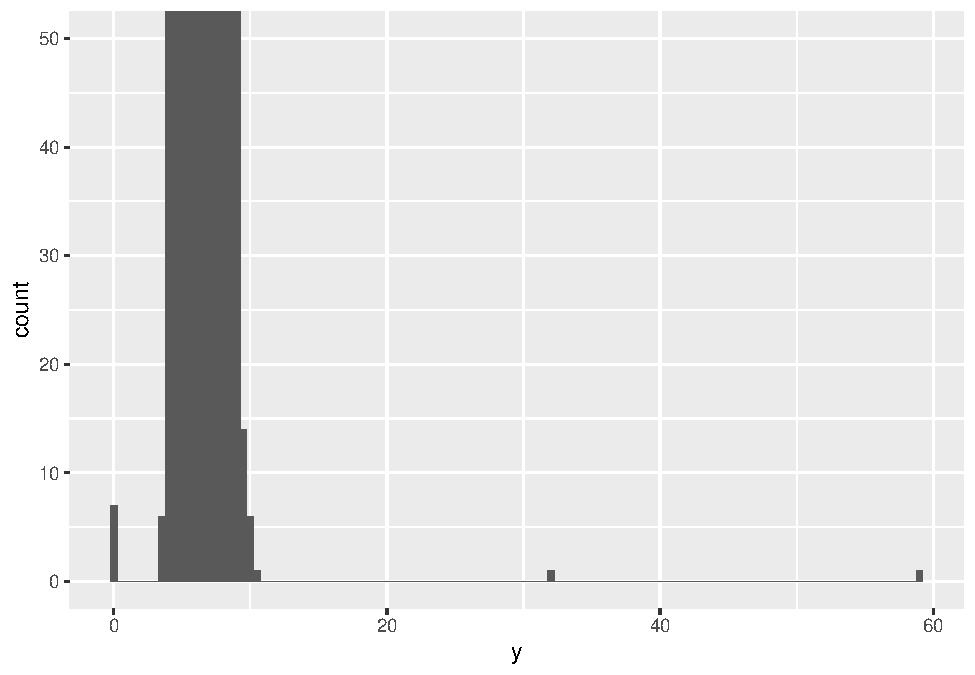
\includegraphics{R_learing_notes_files/figure-latex/unnamed-chunk-236-1} \end{center}

或者,我們也可以使用 \texttt{dplyr},列出寬度小於 3 mm 或超過 20 mm 的觀察值:

\begin{Shaded}
\begin{Highlighting}[]
\NormalTok{unusual }\OtherTok{\textless{}{-}}\NormalTok{ diamonds }\SpecialCharTok{\%\textgreater{}\%}
  \FunctionTok{filter}\NormalTok{(y }\SpecialCharTok{\textless{}} \DecValTok{3} \SpecialCharTok{|}\NormalTok{ y }\SpecialCharTok{\textgreater{}} \DecValTok{20}\NormalTok{) }\SpecialCharTok{\%\textgreater{}\%}
  \FunctionTok{arrange}\NormalTok{(y)}

\NormalTok{unusual}
\end{Highlighting}
\end{Shaded}

\begin{verbatim}
## # A tibble: 9 x 10
##   carat cut       color clarity depth table price     x     y     z
##   <dbl> <ord>     <ord> <ord>   <dbl> <dbl> <int> <dbl> <dbl> <dbl>
## 1  1    Very Good H     VS2      63.3    53  5139  0      0    0   
## 2  1.14 Fair      G     VS1      57.5    67  6381  0      0    0   
## 3  1.56 Ideal     G     VS2      62.2    54 12800  0      0    0   
## 4  1.2  Premium   D     VVS1     62.1    59 15686  0      0    0   
## 5  2.25 Premium   H     SI2      62.8    59 18034  0      0    0   
## 6  0.71 Good      F     SI2      64.1    60  2130  0      0    0   
## 7  0.71 Good      F     SI2      64.1    60  2130  0      0    0   
## 8  0.51 Ideal     E     VS1      61.8    55  2075  5.15  31.8  5.12
## 9  2    Premium   H     SI2      58.9    57 12210  8.09  58.9  8.06
\end{verbatim}

我們可以發現,寬度等於 0 mm 的鑽石根本不可能存在,顯然是打錯了;而寬度為 31.8 mm 與 58.9 mm 那兩個觀察值的價格也不合理。此種錯誤(像是輸入錯誤)所出現的 outliers 就該丟掉。但也不是逢 outliers 就該丟掉,如果其有真實的意義,那還是必須保留。

\hypertarget{missing-value}{%
\section{Missing Value}\label{missing-value}}

\hypertarget{ux66ffux63dbux6389-outliers}{%
\subsection{替換掉 Outliers}\label{ux66ffux63dbux6389-outliers}}

遇到 outliers,有兩種做法:

\begin{enumerate}
\def\labelenumi{\arabic{enumi}.}
\tightlist
\item
  丟棄有奇怪的變數值的觀察值。可是,其中一個變數輸入錯誤不代表其他變數就也輸入錯誤。而且如果資料品質不良,可能最後什麼都不剩。
\end{enumerate}

\begin{Shaded}
\begin{Highlighting}[]
\CommentTok{\# 丟棄有奇怪的變數值的觀察}
\NormalTok{diamonds2 }\OtherTok{\textless{}{-}}\NormalTok{ diamonds }\SpecialCharTok{\%\textgreater{}\%}
  \FunctionTok{filter}\NormalTok{(}\FunctionTok{between}\NormalTok{(y, }\DecValTok{3}\NormalTok{, }\DecValTok{20}\NormalTok{))}
\end{Highlighting}
\end{Shaded}

\begin{enumerate}
\def\labelenumi{\arabic{enumi}.}
\setcounter{enumi}{1}
\tightlist
\item
  (推薦)把 outliers 的變數值換成 \texttt{NA}。我們可以使用 \texttt{mutate()} 與 \texttt{ifelse()},如:
\end{enumerate}

\begin{Shaded}
\begin{Highlighting}[]
\CommentTok{\# 把 outliers 的變數值換成 NA}
\NormalTok{diamonds2 }\OtherTok{\textless{}{-}}\NormalTok{ diamonds }\SpecialCharTok{\%\textgreater{}\%}
  \FunctionTok{mutate}\NormalTok{(}\AttributeTok{y =} \FunctionTok{ifelse}\NormalTok{(y }\SpecialCharTok{\textless{}} \DecValTok{3} \SpecialCharTok{|}\NormalTok{ y }\SpecialCharTok{\textgreater{}} \DecValTok{20}\NormalTok{, }\ConstantTok{NA}\NormalTok{, y))}
\end{Highlighting}
\end{Shaded}

\begin{Shaded}
\begin{Highlighting}[]
\CommentTok{\# 這樣畫出來的散佈圖就不會是 y 的 outliers}
\FunctionTok{ggplot}\NormalTok{(}\AttributeTok{data =}\NormalTok{ diamonds2, }\AttributeTok{mapping =} \FunctionTok{aes}\NormalTok{(}\AttributeTok{x =}\NormalTok{ x, }\AttributeTok{y =}\NormalTok{ y)) }\SpecialCharTok{+}
  \FunctionTok{geom\_point}\NormalTok{(}\AttributeTok{na.rm =} \ConstantTok{TRUE}\NormalTok{)  }\CommentTok{\# 注意:設定 na.rm = TRUE,忽略掉 NA}
\end{Highlighting}
\end{Shaded}

\begin{center}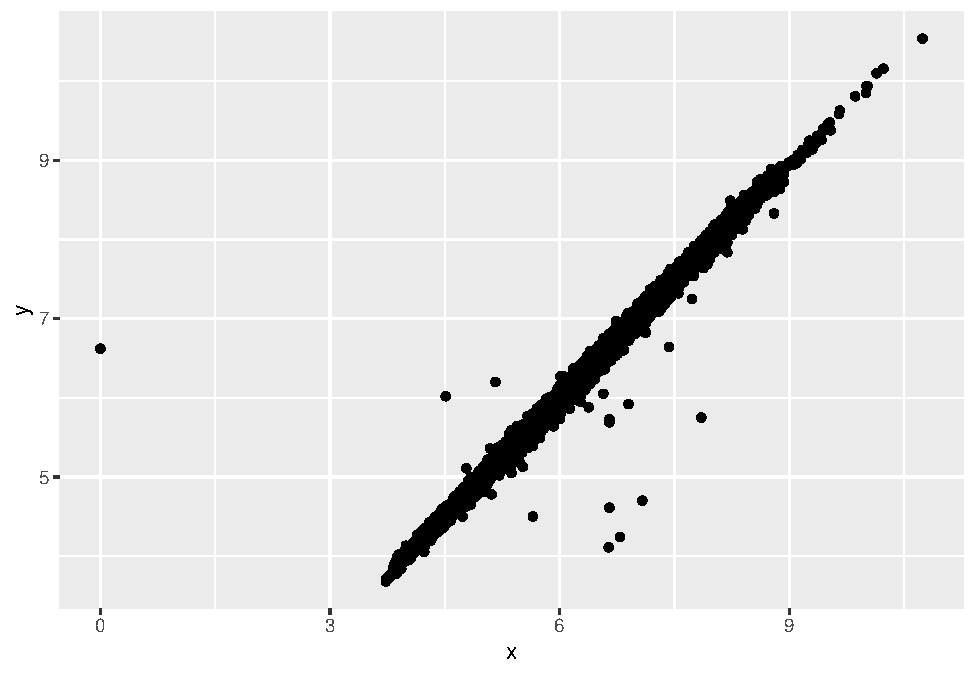
\includegraphics{R_learing_notes_files/figure-latex/unnamed-chunk-240-1} \end{center}

\hypertarget{ux6bd4ux8f03-na-ux8207ux5426}{%
\subsection{\texorpdfstring{比較 \texttt{NA} 與否}{比較 NA 與否}}\label{ux6bd4ux8f03-na-ux8207ux5426}}

有時候我們想了解具有 \texttt{NA} 的觀察值與有變數值的觀察值有何區別,那我們就可以使用 \texttt{mutate()} 與 \texttt{is.na()} 來記錄。在 \texttt{nycflights13} 的 \texttt{flights} 中,\texttt{dep\_time} 如果是 \texttt{NA},那表示航班取消。當我們想要比較取消航班與為取消航班之間的預計離開時間的差別,我們可以:

\begin{Shaded}
\begin{Highlighting}[]
\NormalTok{nycflights13}\SpecialCharTok{::}\NormalTok{flights }\SpecialCharTok{\%\textgreater{}\%}
  \FunctionTok{mutate}\NormalTok{(}
    \AttributeTok{cancelled =} \FunctionTok{is.na}\NormalTok{(dep\_time),}
    \AttributeTok{sched\_hour =}\NormalTok{ sched\_dep\_time }\SpecialCharTok{\%/\%} \DecValTok{100}\NormalTok{,}
    \AttributeTok{sched\_min =}\NormalTok{ sched\_dep\_time }\SpecialCharTok{\%\%} \DecValTok{100}\NormalTok{,}
    \AttributeTok{sched\_dep\_time =}\NormalTok{ sched\_hour }\SpecialCharTok{+}\NormalTok{ sched\_min }\SpecialCharTok{/} \DecValTok{60}\NormalTok{) }\SpecialCharTok{\%\textgreater{}\%}
  \FunctionTok{ggplot}\NormalTok{(}\AttributeTok{mapping =} \FunctionTok{aes}\NormalTok{(sched\_dep\_time)) }\SpecialCharTok{+}
  \FunctionTok{geom\_freqpoly}\NormalTok{(}\AttributeTok{mapping =} \FunctionTok{aes}\NormalTok{(}\AttributeTok{color =}\NormalTok{ cancelled), }\AttributeTok{binwidth =} \DecValTok{1}\SpecialCharTok{/}\DecValTok{4}\NormalTok{)}
\end{Highlighting}
\end{Shaded}

\begin{center}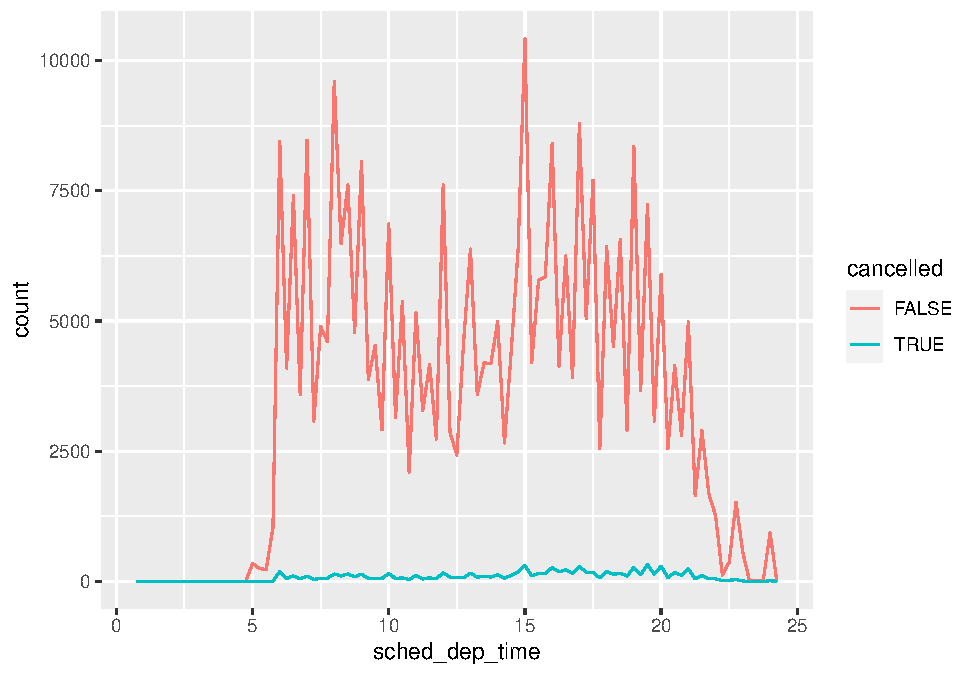
\includegraphics{R_learing_notes_files/figure-latex/unnamed-chunk-241-1} \end{center}

不過,因為未取消航班比取消的航班多太多了,因此下個章節我們要對此做些改進。

\hypertarget{covariation}{%
\section{Covariation}\label{covariation}}

Covariation 即兩個或多個變數變動的關係。想要發覺 covariation,最好的辦法就是視覺化它。但如何視覺化則牽涉到變數型態的問題。

\hypertarget{ux985eux5225ux8207ux9023ux7e8cux8b8aux6578}{%
\subsection{類別與連續變數}\label{ux985eux5225ux8207ux9023ux7e8cux8b8aux6578}}

\begin{quote}
為什麼我們剛剛所使用的 \texttt{geom\_freqpoly()} 不太適合拿來「比較」變數?
\end{quote}

這是因為,\texttt{geom\_freqpoly()} 的高度(縱軸)是出現次數,所以說如果有一組遠小於另一組,像剛剛的情況,那我們就很難看出其形狀的差異。以下還有另一個例子為比較不同品質的鑽石之間的價格差異:

\begin{Shaded}
\begin{Highlighting}[]
\FunctionTok{ggplot}\NormalTok{(}\AttributeTok{data =}\NormalTok{ diamonds, }\AttributeTok{mapping =} \FunctionTok{aes}\NormalTok{(}\AttributeTok{x =}\NormalTok{ price)) }\SpecialCharTok{+}
  \FunctionTok{geom\_freqpoly}\NormalTok{(}\AttributeTok{mapping =} \FunctionTok{aes}\NormalTok{(}\AttributeTok{color =}\NormalTok{ cut), }\AttributeTok{binwidth =} \DecValTok{500}\NormalTok{)}
\end{Highlighting}
\end{Shaded}

\begin{center}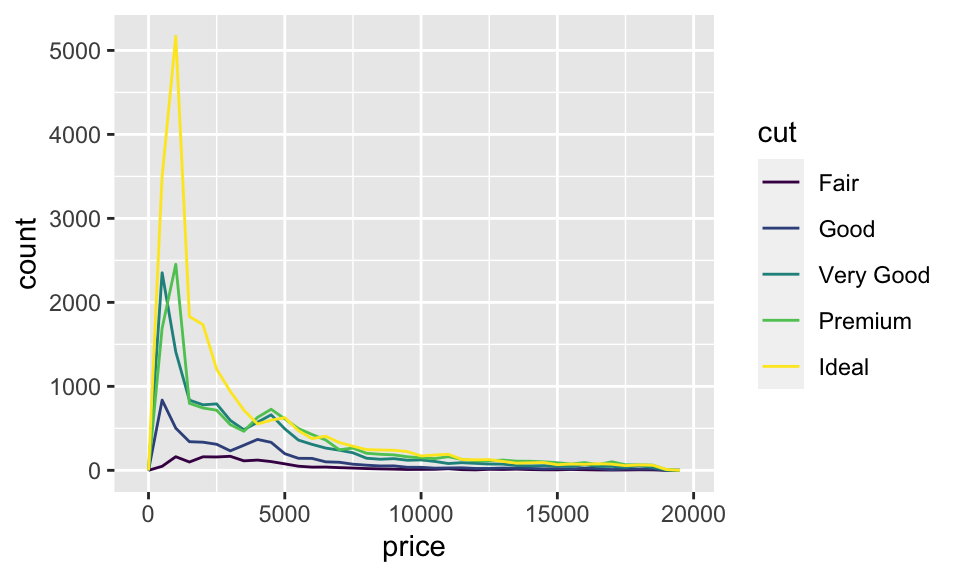
\includegraphics{R_learing_notes_files/figure-latex/unnamed-chunk-242-1} \end{center}

這種時候,我們可以把 \(y\) 軸從呈現 ``count'',改成呈現 ``density'',即經過標準化的 count,在每組的多邊形底下的面積都為 \(1\),如:

\begin{Shaded}
\begin{Highlighting}[]
\FunctionTok{ggplot}\NormalTok{(}\AttributeTok{data =}\NormalTok{ diamonds, }\AttributeTok{mapping =} \FunctionTok{aes}\NormalTok{(}\AttributeTok{x =}\NormalTok{ price, }\AttributeTok{y =}\NormalTok{ ..density..)) }\SpecialCharTok{+}
  \FunctionTok{geom\_freqpoly}\NormalTok{(}\AttributeTok{mapping =} \FunctionTok{aes}\NormalTok{(}\AttributeTok{color =}\NormalTok{ cut), }\AttributeTok{binwidth =} \DecValTok{500}\NormalTok{)}
\end{Highlighting}
\end{Shaded}

\begin{center}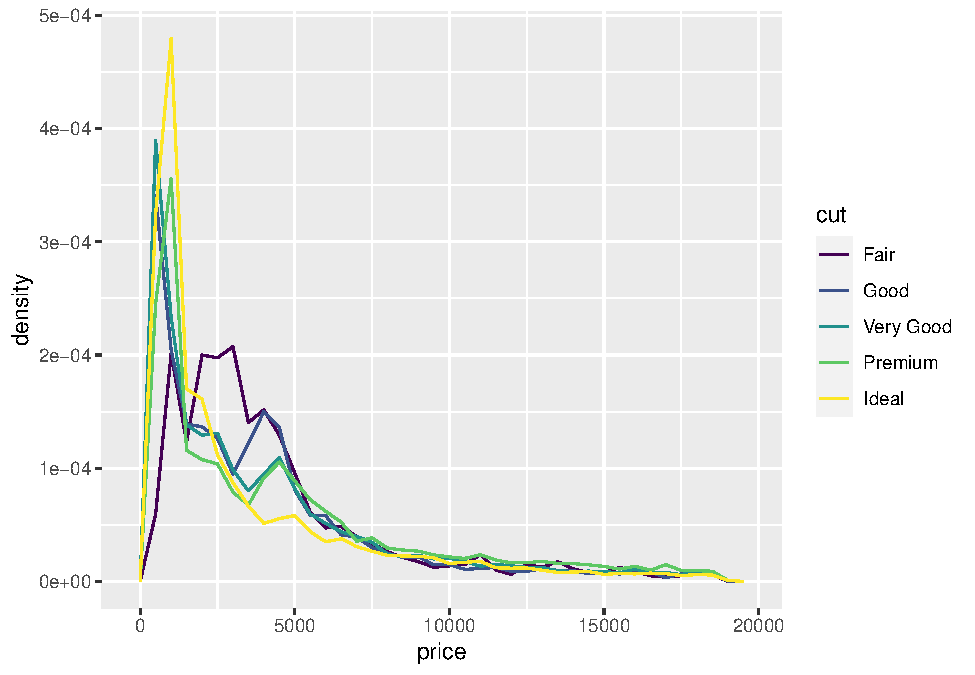
\includegraphics{R_learing_notes_files/figure-latex/unnamed-chunk-243-1} \end{center}

另一種把連續變數拆成類別變數然後呈現的方法是使用箱形圖(box plot),其可以把某些分佈的特徵給視覺化;即每個箱形圖中的箱子的底部都是 25 百分位,而頂部都是 75 百分位,箱子的中間則是中位數。我們可以大略看出分佈與偏態,而箱形圖中的點則是 outliers,線則是從箱子外延伸到非 outliers 的地方,如:

\begin{Shaded}
\begin{Highlighting}[]
\FunctionTok{ggplot}\NormalTok{(}\AttributeTok{data =}\NormalTok{ diamonds, }\AttributeTok{mapping =} \FunctionTok{aes}\NormalTok{(}\AttributeTok{x =}\NormalTok{ cut, }\AttributeTok{y =}\NormalTok{ price)) }\SpecialCharTok{+}
  \FunctionTok{geom\_boxplot}\NormalTok{()}
\end{Highlighting}
\end{Shaded}

\begin{center}\includegraphics{R_learing_notes_files/figure-latex/unnamed-chunk-244-1} \end{center}

\hypertarget{ux5169ux500bux985eux5225ux8b8aux6578}{%
\subsection{兩個類別變數}\label{ux5169ux500bux985eux5225ux8b8aux6578}}

\hypertarget{ux5169ux500bux9023ux7e8cux8b8aux6578}{%
\subsection{兩個連續變數}\label{ux5169ux500bux9023ux7e8cux8b8aux6578}}

\hypertarget{ux6a21ux5f0fux8207ux6a21ux578b}{%
\section{模式與模型}\label{ux6a21ux5f0fux8207ux6a21ux578b}}

\hypertarget{ggplot2-calls}{%
\section{ggplot2 Calls}\label{ggplot2-calls}}

\hypertarget{part-ux4ee5-tidyverse-ux9032ux884cux8cc7ux6599ux6574ux7406}{%
\chapter*{\texorpdfstring{(PART) 以 \texttt{tidyverse} 進行資料整理}{(PART) 以 tidyverse 進行資料整理}}\label{part-ux4ee5-tidyverse-ux9032ux884cux8cc7ux6599ux6574ux7406}}

\hypertarget{ux4ee5-tibble-ux8655ux7406-tibbles}{%
\chapter{\texorpdfstring{以 \texttt{tibble} 處理 Tibbles}{以 tibble 處理 Tibbles}}\label{ux4ee5-tibble-ux8655ux7406-tibbles}}

\hypertarget{ux4ee5-readr-ux532fux5165ux8cc7ux6599}{%
\chapter{\texorpdfstring{以 \texttt{readr} 匯入資料}{以 readr 匯入資料}}\label{ux4ee5-readr-ux532fux5165ux8cc7ux6599}}

\hypertarget{tidyr}{%
\chapter{\texorpdfstring{以 \texttt{tidyr} 整理資料}{以 tidyr 整理資料}}\label{tidyr}}

\hypertarget{ux4ee5-dplyr-ux8655ux7406ux95dcux806fux6027ux8cc7ux6599}{%
\chapter{\texorpdfstring{以 \texttt{dplyr} 處理關聯性資料}{以 dplyr 處理關聯性資料}}\label{ux4ee5-dplyr-ux8655ux7406ux95dcux806fux6027ux8cc7ux6599}}

\hypertarget{stringr}{%
\chapter{\texorpdfstring{以 \texttt{stringr} 處理字串}{以 stringr 處理字串}}\label{stringr}}

\hypertarget{ux4ee5-forcats-ux8655ux7406-factors}{%
\chapter{\texorpdfstring{以 \texttt{forcats} 處理 Factors}{以 forcats 處理 Factors}}\label{ux4ee5-forcats-ux8655ux7406-factors}}

\hypertarget{ux4ee5-lubridate-ux8655ux7406ux65e5ux671fux6642ux9593}{%
\chapter{\texorpdfstring{以 \texttt{lubridate} 處理日期時間}{以 lubridate 處理日期時間}}\label{ux4ee5-lubridate-ux8655ux7406ux65e5ux671fux6642ux9593}}

\hypertarget{part-ux7de8ux5bebux7a0bux5f0fux8207-tidyverse}{%
\chapter*{\texorpdfstring{(PART) 編寫程式與 \texttt{tidyverse}}{(PART) 編寫程式與 tidyverse}}\label{part-ux7de8ux5bebux7a0bux5f0fux8207-tidyverse}}

\hypertarget{ux4ee5-magrittr-ux4f7fux7528-pipes}{%
\chapter{\texorpdfstring{以 \texttt{magrittr} 使用 Pipes}{以 magrittr 使用 Pipes}}\label{ux4ee5-magrittr-ux4f7fux7528-pipes}}

\hypertarget{part-ux7db2ux8defux8207ux8cc7ux6599ux6280ux8853ux5165ux9580}{%
\part{網路與資料技術入門}\label{part-ux7db2ux8defux8207ux8cc7ux6599ux6280ux8853ux5165ux9580}}

\hypertarget{html}{%
\chapter{HTML}\label{html}}

HTML 為 the \textbf{H}yper\textbf{T}ext \textbf{M}arkup \textbf{L}anguage 的縮寫。

\begin{itemize}
\item
  在節 \ref{sourcecode},將會使用瀏覽器呈現網頁原始碼(source code),並查看特定的 HTML 元素。
\item
  在節 \ref{htmlsyntax},將會介紹標記語言的邏輯與 HTML 的語法規則。
\item
  在節 \ref{tagsattri},將會呈現 HTML 最重要的詞彙。
\item
  在節 \ref{parsing},將會討論重構 HTML 結構及語法的過程,即\textbf{解析(parsing)},與其如何幫助我們從網頁文檔提取資訊。
\end{itemize}

\hypertarget{sourcecode}{%
\section{瀏覽器呈現與原始碼}\label{sourcecode}}

HTML 檔為純文字檔(plain text file)。HTML markup 可以用來定義文檔哪些部分該是標題、連結、表格,或其他格式。這些標記會告訴瀏覽器文檔如何組織,與其各部分的功能。

我們在網頁瀏覽器中所看到過的是轉譯過的 HTML 檔,例如網頁 \url{http://www.r-datacollection.com/materials/html/OurFirstHTML.html} ,呈現在我們眼前的是一句話:``I am your first HTML-file!'',而實際上有如此的原始碼:

\begin{Shaded}
\begin{Highlighting}[]
\DataTypeTok{\textless{}!DOCTYPE }\NormalTok{html}\DataTypeTok{\textgreater{}}
 \KeywordTok{\textless{}html\textgreater{}}
   \KeywordTok{\textless{}head\textgreater{}}
     \KeywordTok{\textless{}title\textgreater{}}\NormalTok{First HTML}\KeywordTok{\textless{}/title\textgreater{}}  \CommentTok{\textless{}!{-}{-} 此網頁的 title {-}{-}\textgreater{}}  
   \KeywordTok{\textless{}/head\textgreater{}}
   \KeywordTok{\textless{}body\textgreater{}}
\NormalTok{     I am your first HTML{-}file!}
   \KeywordTok{\textless{}/body\textgreater{}}
 \KeywordTok{\textless{}/html\textgreater{}}
\end{Highlighting}
\end{Shaded}

\hypertarget{htmlsyntax}{%
\section{語法規則}\label{htmlsyntax}}

\hypertarget{ux6a19ux7c64ux5143ux7d20ux8207ux5c6cux6027}{%
\subsection{標籤、元素與屬性}\label{ux6a19ux7c64ux5143ux7d20ux8207ux5c6cux6027}}

透過可以被瀏覽器讀懂的\textbf{標籤(tags)},純文字檔可以變成 HTML 文件。

標籤由 \texttt{\textless{}} 與 \texttt{\textgreater{}} 包著,分成兩種,其一為 start tags,又稱為 opening tags,例如 \texttt{\textless{}title\textgreater{}};其二為 end tags,又稱為 closing tags,與 start tags 不同的是多了 \texttt{/},如 \texttt{\textless{}/title\textgreater{}}。

\textbf{元素(elements)}則包含 start tags、contents 與 end tags,\footnote{不過標籤與元素常常被當成同義詞就是了,以後我們也會這麼做。}如:

\begin{Shaded}
\begin{Highlighting}[]
\KeywordTok{\textless{}title\textgreater{}}\NormalTok{First HTML}\KeywordTok{\textless{}/title\textgreater{}}
\end{Highlighting}
\end{Shaded}

不過,並非所有的元素都會有一個 start tag 與一個 end tag。例如 \texttt{\textless{}br\textgreater{}} 意思是換行,就不會有另一個 \texttt{\textless{}/br\textgreater{}} 為 end tag。如果元素形為 \texttt{\textless{}body/\textgreater{}},在 start tag 中就以 \texttt{/} 結束,則稱為\textbf{空元素},因為沒有任何 content。HTML 的標籤的大小寫並不重要,因此 \texttt{\textless{}tagNAME\textgreater{}}、\texttt{\textless{}TAGNAME\textgreater{}} 或 \texttt{\textless{}tagname\textgreater{}} 都是等價的,但一般我們會寫成全部都是小寫的形式。

此外,標籤還有一特色為\textbf{屬性(attributes)},通常放在 start tag 的標籤名稱之後。一個屬性會有一個屬性名稱與一個值,例如:

\begin{Shaded}
\begin{Highlighting}[]
\KeywordTok{\textless{}a}\OtherTok{ href=}\StringTok{"http://www.r{-}datacollection.com/"}\KeywordTok{\textgreater{}}\NormalTok{Link to Homepage}\KeywordTok{\textless{}/a\textgreater{}}
\end{Highlighting}
\end{Shaded}

其中的 \texttt{href="http://www.r-datacollection.com/"}就是指定 anchor \texttt{\textless{}a\textgreater{}} 的屬性,而 \texttt{href} 就是屬性名稱,以單引號或雙引號包著的 \texttt{"http://www.r-datacollection.com/"} 即是屬性的值。標籤也能有多個屬性,只要用空格隔開即可。

\hypertarget{ux6a39ux7d50ux69cb}{%
\subsection{樹結構}\label{ux6a39ux7d50ux69cb}}

\begin{Shaded}
\begin{Highlighting}[]
\DataTypeTok{\textless{}!DOCTYPE }\NormalTok{html}\DataTypeTok{\textgreater{}}
 \KeywordTok{\textless{}html\textgreater{}}
   \KeywordTok{\textless{}head\textgreater{}}
     \KeywordTok{\textless{}title\textgreater{}}\NormalTok{First HTML}\KeywordTok{\textless{}/title\textgreater{}}
   \KeywordTok{\textless{}/head\textgreater{}}
   \KeywordTok{\textless{}body\textgreater{}}
\NormalTok{     I am your first HTML{-}file!}
   \KeywordTok{\textless{}/body\textgreater{}}
 \KeywordTok{\textless{}/html\textgreater{}}
\end{Highlighting}
\end{Shaded}

以上述範例而言,\texttt{html} 包著 \texttt{\textless{}head\textgreater{}} 與 \texttt{\textless{}body\textgreater{}},\texttt{\textless{}head\textgreater{}} 則包著 \texttt{\textless{}title\textgreater{}},就像\textbf{樹結構(tree structure)}一樣,如圖 \ref{fig:treestructure}。

\begin{figure}

{\centering \includegraphics[width=400]{images/截圖 2021-07-28 下午5.31.14} 

}

\caption{樹結構。}\label{fig:treestructure}
\end{figure}

\hypertarget{ux8a3bux91cb}{%
\subsection{註釋}\label{ux8a3bux91cb}}

HTML 可以加入\textbf{註釋(comments)},以 \texttt{\textless{}!-\/-} 開頭,\texttt{-\/-\textgreater{}} 結尾,中間的文字會被忽略,不會被呈現在瀏覽器上,如:

\begin{Shaded}
\begin{Highlighting}[]
\CommentTok{\textless{}!{-}{-} Hi, I am a comment.}
\CommentTok{I can span several lines and I am able to store additional}
\CommentTok{  content that is not displayed by the browser. {-}{-}\textgreater{}}
\end{Highlighting}
\end{Shaded}

\hypertarget{ux4fddux7559ux8207ux7279ux6b8aux5b57ux5143}{%
\subsection{保留與特殊字元}\label{ux4fddux7559ux8207ux7279ux6b8aux5b57ux5143}}

\begin{quote}
HTML 的標籤使用 \texttt{\textless{}} 與 \texttt{\textgreater{}},那我們要在正文使用 \textless{} 或 \textgreater{} 時怎麼辦?
\end{quote}

對於這些會在 HTML 語法中使用的字元,如果要在 content 中使用它們,就要透過對應的 \textbf{character entities}。Entities 以 \texttt{\&} 開頭,以 \texttt{;} 結尾。例如,如果我們希望瀏覽器可以顯示 ``5 \textless{} 6 but 7 \textgreater{} 3'',不應該使用

\begin{Shaded}
\begin{Highlighting}[]
\KeywordTok{\textless{}p\textgreater{}}\NormalTok{5 }\ErrorTok{\textless{}}\NormalTok{ 6 but 7 \textgreater{} 3 }\KeywordTok{\textless{}/p\textgreater{}}
\end{Highlighting}
\end{Shaded}

而應該使用

\begin{Shaded}
\begin{Highlighting}[]
\KeywordTok{\textless{}p\textgreater{}}\NormalTok{5 }\DecValTok{\&lt;}\NormalTok{ 6 but 7 }\DecValTok{\&gt;}\NormalTok{ 3 }\KeywordTok{\textless{}/p\textgreater{}}
\end{Highlighting}
\end{Shaded}

\begin{longtable}[]{@{}
  >{\raggedright\arraybackslash}p{(\columnwidth - 6\tabcolsep) * \real{0.10}}
  >{\raggedright\arraybackslash}p{(\columnwidth - 6\tabcolsep) * \real{0.22}}
  >{\raggedright\arraybackslash}p{(\columnwidth - 6\tabcolsep) * \real{0.19}}
  >{\raggedright\arraybackslash}p{(\columnwidth - 6\tabcolsep) * \real{0.31}}@{}}
\caption{\label{tab:htmlentities} HTML entities.}\tabularnewline
\toprule
字元 & Entity number & Entity name & 意思 \\
\midrule
\endfirsthead
\toprule
字元 & Entity number & Entity name & 意思 \\
\midrule
\endhead
" & \texttt{\&\#34;} & \texttt{\&quot;} & quotation mark \\
' & \texttt{\&\#39;} & \texttt{\&apos;} & apostrophe \\
\& & \texttt{\&\#38;} & \texttt{\&amp;} & ampersand \\
\textless{} & \texttt{\&\#60;} & \texttt{\&lt;} & less than \\
\textgreater{} & \texttt{\&\#62;} & \texttt{\&gt;} & greater than \\
& \texttt{\&\#160;} & \texttt{\&nbsp;} & non-breaking space \\
á & \texttt{\&\#224;} & \texttt{\&agrave;} & a with grave accent \\
♡ & \texttt{\&\#224;} & \texttt{\&hearts;} & heart \\
\bottomrule
\end{longtable}

\hypertarget{ux6587ux4ef6ux985eux578bux5b9aux7fa9}{%
\subsection{文件類型定義}\label{ux6587ux4ef6ux985eux578bux5b9aux7fa9}}

\hypertarget{ux7a7aux767dux8207ux63dbux884c}{%
\subsection{空白與換行}\label{ux7a7aux767dux8207ux63dbux884c}}

\hypertarget{tagsattri}{%
\section{標籤與屬性}\label{tagsattri}}

\hypertarget{the-anchor-tag-a}{%
\subsection{\texorpdfstring{The anchor tag \texttt{\textless{}a\textgreater{}}}{The anchor tag \textless a\textgreater{}}}\label{the-anchor-tag-a}}

\hypertarget{the-metadata-tag-meta}{%
\subsection{\texorpdfstring{The metadata tag \texttt{\textless{}meta\textgreater{}}}{The metadata tag \textless meta\textgreater{}}}\label{the-metadata-tag-meta}}

\hypertarget{the-external-reference-tag-link}{%
\subsection{\texorpdfstring{The external reference tag \texttt{\textless{}link\textgreater{}}}{The external reference tag \textless link\textgreater{}}}\label{the-external-reference-tag-link}}

\hypertarget{emphasizing-tags-b-i-strong}{%
\subsection{\texorpdfstring{Emphasizing tags \texttt{\textless{}b\textgreater{}}, \texttt{\textless{}i\textgreater{}}, \texttt{\textless{}strong\textgreater{}}}{Emphasizing tags \textless b\textgreater, \textless i\textgreater, \textless strong\textgreater{}}}\label{emphasizing-tags-b-i-strong}}

\hypertarget{the-paragraphs-tag-p}{%
\subsection{\texorpdfstring{The paragraphs tag \texttt{\textless{}p\textgreater{}}}{The paragraphs tag \textless p\textgreater{}}}\label{the-paragraphs-tag-p}}

\hypertarget{heading-tags-h1-h2-h3}{%
\subsection{\texorpdfstring{Heading tags \texttt{\textless{}h1\textgreater{}}, \texttt{\textless{}h2\textgreater{}}, \texttt{\textless{}h3\textgreater{}},\ldots{}}{Heading tags \textless h1\textgreater, \textless h2\textgreater, \textless h3\textgreater,\ldots{}}}\label{heading-tags-h1-h2-h3}}

\hypertarget{listing-content-with-ul-ol-and-dl}{%
\subsection{\texorpdfstring{Listing content with \texttt{\textless{}ul\textgreater{}}, \texttt{\textless{}ol\textgreater{}}, and \texttt{\textless{}dl\textgreater{}}}{Listing content with \textless ul\textgreater, \textless ol\textgreater, and \textless dl\textgreater{}}}\label{listing-content-with-ul-ol-and-dl}}

\hypertarget{the-organizational-tags-div-and-span}{%
\subsection{\texorpdfstring{The organizational tags \texttt{\textless{}div\textgreater{}} and \texttt{\textless{}span\textgreater{}}}{The organizational tags \textless div\textgreater{} and \textless span\textgreater{}}}\label{the-organizational-tags-div-and-span}}

\hypertarget{the-form-tag-and-its-companions}{%
\subsection{\texorpdfstring{The \texttt{\textless{}form\textgreater{}} tag and its companions}{The \textless form\textgreater{} tag and its companions}}\label{the-form-tag-and-its-companions}}

\hypertarget{the-foreign-script-tag-script}{%
\subsection{\texorpdfstring{The foreign script tag \texttt{\textless{}script\textgreater{}}}{The foreign script tag \textless script\textgreater{}}}\label{the-foreign-script-tag-script}}

\hypertarget{table-tags-table-tr-td-and-th}{%
\subsection{\texorpdfstring{Table tags \texttt{\textless{}table\textgreater{}}, \texttt{\textless{}tr\textgreater{}}, \texttt{\textless{}td\textgreater{}}, and \texttt{\textless{}th\textgreater{}}}{Table tags \textless table\textgreater, \textless tr\textgreater, \textless td\textgreater, and \textless th\textgreater{}}}\label{table-tags-table-tr-td-and-th}}

\hypertarget{parsing}{%
\section{解析}\label{parsing}}

\hypertarget{discarding-nodes}{%
\subsection{Discarding nodes}\label{discarding-nodes}}

\hypertarget{ux63d0ux53d6ux8cc7ux8a0a}{%
\subsection{提取資訊}\label{ux63d0ux53d6ux8cc7ux8a0a}}

\hypertarget{xml-ux8207-json}{%
\chapter{XML 與 JSON}\label{xml-ux8207-json}}

\hypertarget{xpath}{%
\chapter{XPath}\label{xpath}}

\hypertarget{http}{%
\chapter{HTTP}\label{http}}

\hypertarget{ajax}{%
\chapter{AJAX}\label{ajax}}

\hypertarget{sql-ux8207ux76f8ux95dcux7684ux8cc7ux6599ux5eab}{%
\chapter{SQL 與相關的資料庫}\label{sql-ux8207ux76f8ux95dcux7684ux8cc7ux6599ux5eab}}

\hypertarget{ux6b63ux898fux8868ux9054ux5f0f}{%
\chapter{正規表達式}\label{ux6b63ux898fux8868ux9054ux5f0f}}

\hypertarget{part-ux7db2ux8defux722cux87f2ux8207ux6587ux5b57ux63a2ux52d8}{%
\part{網路爬蟲與文字探勘}\label{part-ux7db2ux8defux722cux87f2ux8207ux6587ux5b57ux63a2ux52d8}}

\hypertarget{ux7db2ux8defux722cux87f2}{%
\chapter{網路爬蟲}\label{ux7db2ux8defux722cux87f2}}

  \bibliography{我的文獻庫.bib}

\end{document}
